\bookpart{多元微积分}{Multivariate Calculus}
\label{part:multivariate-calculus}

\BookPartGuide{%
前三部分研究的是线性作用：矩阵把一个向量映为另一个向量，误差按固定的倍数放大。本部分研究一般的多元映射，主线有两条：怎样描述它在一点附近的局部变化，以及怎样在区域、曲线和曲面上累计一个量。

前四章处理局部变化。多元函数微分章把函数看作位置上的标量场与向量场，用全微分统一预测所有方向的一阶变化，梯度、Jacobian与Hessian分别记录标量输出、向量输出和二阶弯曲。矩阵函数的微分章以矩阵为自变量，给出乘积、求逆、行列式与对数行列式的微分公式和梯度。

隐函数与反函数章从方程出发，说明关于待解变量的Jacobian可逆时，方程在局部确定唯一的可微解。微分与扰动分析章把这三章的工具与谱分析部分的有限扰动界结合起来，研究指定方向的一阶响应、误差的局部放大倍数和线性预测的余项，并用于矩阵运算和隐式给定的谱分支。

后四章处理累计。区域积分章用分割和定义多维Riemann积分，再以累次积分、换元和参数积分计算它。路径积分章与曲面积分章分别按弧长和面积累计标量场，又按切向和法向累计向量场，得到功、环流与通量。积分定理章用散度与旋度描述局部的净流出与环流，再由Green、Gauss和Stokes公式把内部的导数累计与边界上的累计联系起来。

阅读时要分清几组容易混淆的对象：线性映射形式的微分与表示它的梯度或矩阵；指定方向的变化率、最坏方向的条件数与有限步长的余项；局部可逆与整体单射；按长度、面积等非负权重的累计与依赖方向或法向的累计。每个结论都带有定义域、光滑性、覆盖次数或定向的条件，使用时要逐项核对。}

\chapter{多元函数微分}
\label{chap:multivariate-differentiation}
\label{chap:multivariate-calculus}
\label{chap:multivariable-functions}

一元微分研究输入改变一点时输出改变多少：导数$f'(a)$是输出改变量与输入改变量之比的极限。许多量却同时依赖多个输入。平板上一点的温度由横、纵两个坐标决定，模型的损失由大量参数决定，流体的速度则在空间每一点给出一个向量。

以$f(x,y)=x^2+xy+y^2$为例，输入是平面上的点$(x,y)$，输出是一个实数。把$z=f(x,y)$看成地形的高度，把$(x,y)$看成地图上的位置。从一点出发，可以向东走、向北走、斜着走，也可以沿一条弯曲的路线靠近。本章要回答的问题是：能否用一个线性映射统一预测所有这些走法下的输出变化；这个预测在什么条件下成立；它的弯曲部分又怎样决定一点附近的形状，例如驻点是谷底、山顶还是鞍点。

第~\ref{chap:normed-inner-product-spaces}章已经建立了收敛、极限与连续性，证明了有限维空间中范数等价、完备，并定义了算子范数；伴随在第~\ref{chap:dual-spaces}章定义；第~\ref{chap:linear-representation}章给出了线性映射、多线性映射与对偶空间。这些是本章的语言。本章新增的问题是：能否把精确变化$f(\bm a+\bm h)-f(\bm a)$分成对$\bm h$线性的一阶部分和更小的余项。函数连续、有限变化有界，都不保证这样的分解存在。

各节按“对象—一阶—向量输出—高阶”的次序展开。第一节把多元函数看作位置上的标量场与向量场，回顾极限与连续性的要点。第二节从坐标方向的变化率出发，判断偏导数与方向导数何时组成全微分，再用内积把全微分表示为梯度，并用中值估计控制有限变化。

第三节把输出扩大为向量，用Jacobian矩阵记录微分，用链式法则组合复杂映射，并用导数的算子范数估计向量增量。第四节把微分再用于梯度，得到Hessian和多元Taylor公式，并据此判断驻点附近的形状；判断定性时要用到第~\ref{chap:eigen-spectral-decomposition}章的实对称谱分解。

本章只建立微分及其局部结论。以矩阵为自变量的微分在第~\ref{chap:matrix-differentiation}章，由方程隐式确定的函数在第~\ref{chap:implicit-inverse-functions}章；导数怎样控制误差放大、一阶预测在有限步长下还差多少，集中在第~\ref{chap:differential-perturbation-analysis}章。本章还沿用第~\ref{chap:linear-operations}章的向量、矩阵与行列式，以及一元微分的结论，可参考\BookChapterRef{chap:univariate-differentiation}{卷一“一元函数的微分”章}。偏导数与局部线性近似的直观介绍可参考\scite{math-openstax-calculus3}，严格的多元微分论证可参考\scite{math-lebl2026analysis2}。

\par\Needspace{14\baselineskip}

\label{sec:analysis-multivariable-differentiation}
\label{sec:multivariable-differentiation}

\section{多元函数与场}
\label{sec:multivariable-functions-and-fields}

微分和积分都要先说清研究的是什么函数。本部分最常见的情形是：空间中每个位置都带着一个可以测量的量。平板上每一点有温度，河水中每一点有流速，金属块中每一点有密度。这样的量随位置变化，输入是位置的坐标，输出是该位置上读出的量。

第~\ref{sec:multivariable-joint-limit-section}节已经从极限的角度定义了多元标量函数与向量值映射。本节换一个角度，把它们看作空间位置上的属性：先按输出是一个数还是一个向量，区分标量场与向量场；再说明本部分的定义域、输出空间以及极限与连续性怎样理解。这些约定确定了后面各章微分与累计的对象。

\subsection{标量场}
\label{sec:multivariable-scalar-fields}

温度计放在平板的不同位置，读数不同；把每个位置与它的读数配对，就得到一个函数。密度、压强、电势也都在每个位置给出一个实数。这类函数在每个位置只给出大小，不带方向。
\begin{definition}[标量场]
\label{def:multivariable-scalar-field}
设$\Omega\subseteq\mathbb R^d$。映射$f:\Omega\to\mathbb R$称为$\Omega$上的\term{标量场}（scalar field）；它把每个位置$\bm x\in\Omega$映为一个实数$f(\bm x)$。
\end{definition}
作为映射，标量场就是定义~\ref{def:multivariable-scalar-function}中的多元标量函数。“场”这个名称只强调输入是空间位置、输出是该位置的属性。后面称它为多元函数还是标量场，取决于讨论的是一般的输入输出关系，还是位置上的物理量，数学内容相同。

以$f(x,y)=x^2+y^2$为例，它在每个位置给出到原点距离的平方。它有两种画法。第一种画法把函数值当作高度，得到三维空间中的曲面$z=x^2+y^2$，形状像一只碗。第二种画法留在输入平面里，画出等值曲线$\{(x,y):x^2+y^2=c\}$。

对这个函数，$c>0$时等值曲线是半径为$\sqrt c$的圆，$c=0$时只剩原点，$c<0$时是空集。取$c=1,2,3,4$，半径依次为$1,\sqrt2\approx1.41,\sqrt3\approx1.73,2$，相邻两圈的间距越来越小。函数值每增加$1$所需走的距离越来越短，说明离原点越远，场值沿径向增长得越快。

这一观察还只是定性的。度量“沿某方向增长多快”需要导数：第~\ref{sec:multivariable-gradient-inner-product}节把它写成梯度，并说明梯度与等值曲线正交。

\subsection{向量场}
\label{sec:multivariable-vector-fields}

河水在每一点有流速，物体在重力场或电场中的每一点受力。这些量既有大小又有方向，并且与位置同处一个空间：流速可以画成从该点出发的箭头。
\begin{definition}[向量场]
\label{def:multivariable-vector-field}
设$\Omega\subseteq\mathbb R^d$。映射$\bm F:\Omega\to\mathbb R^d$称为$\Omega$上的\term{向量场}（vector field）。按本书约定，$\bm F(\bm x)$写成$d\times1$列矩阵$(F_1(\bm x),\ldots,F_d(\bm x))^\top$，每个分量$F_i:\Omega\to\mathbb R$都是标量场。
\end{definition}
向量场的输入是位置，输出是放在该位置的一个向量。例如$\bm F(x,y)=(x,y)^\top$的箭头从原点向外，离原点越远越长；$\bm F(x,y)=(-y,x)^\top$的箭头与以原点为圆心的圆相切，按逆时针方向。第~\ref{chap:path-integrals}章用这两个场比较沿路径做的功。

向量场是向量值函数的特例。一般向量值函数$F:\Omega\subseteq\mathbb R^d\to\mathbb R^m$的输出维数$m$可以与输入维数不同：参数曲线把一个参数映为空间中的点，神经网络的一层把输入向量映为另一维数的向量。向量场要求$m=d$，输出向量才能画成输入空间中的箭头，也才能与路径的切向量或曲面的法向量作内积。

输出还可以是矩阵。若每个位置给出一个$p\times q$矩阵，例如介质中每一点的应力矩阵，就得到矩阵值的场；它的每个元素仍是标量场。第~\ref{chap:matrix-differentiation}章研究的则是另一种情形：输入本身是矩阵，例如$\bm X\mapsto\bm X^{-1}$。判断一个映射属于哪一类时，要分别核对输入空间和输出空间，不能只看表达式里是否出现矩阵。

\subsection{多元函数的极限与连续}
\label{sec:multivariable-field-limits-continuity}

标量场和向量场的极限与连续性已在第~\ref{chap:normed-inner-product-spaces}章建立，这里只回顾后面要用的结论，不重复证明。

极限用输入、输出空间的范数定义（定义~\ref{def:multivariable-limit}）。$\lim_{\bm x\to\bm a}F(\bm x)=\bm L$的意思是：只要输入进入以$\bm a$为心的某个去心小球，输出与$\bm L$的距离就小于给定误差，不论输入沿什么路线进入。连续性（定义~\ref{def:multivariable-scalar-continuity}）要求这个极限等于$F(\bm a)$。

对有限维的向量输出，这些判断可以逐分量进行：向量场或矩阵值的场在一点有极限或连续，当且仅当每个输出分量如此（定理~\ref{thm:multivariable-coordinatewise-convergence}）。逐分量分解的是输出。输入的多个坐标不能这样拆开，因为输入可以同时改变全部坐标、沿弯曲的路线趋近。

因此，沿路径检验只能用来否定极限。沿两条路径得到不同的极限值，联合极限就不存在：示例~\ref{ex:multivariable-path-limits}中的$xy/(x^2+y^2)$沿$x$轴趋于$0$，沿$y=x$趋于$1/2$。反过来，只检查若干条路径不能证明极限存在：示例~\ref{ex:multivariable-parabola-path-limit}中的$x^2y/(x^4+y^2)$沿每条直线都趋于$0$，沿抛物线$y=x^2$却恒为$1/2$。要证明极限存在，需要一个只依赖输入到基点距离的统一误差估计。

这个区别在微分中还会出现。方向导数是沿固定直线取的极限，全微分则要求误差对全部趋近方式统一受控；第~\ref{sec:multivariable-total-differentiation}节的反例与上面的抛物线例子结构相同。

最后约定定义域。讨论微分时，基点取在开集内部，从基点出发向任何方向走足够小的一步都不离开定义域；讨论积分时，累计范围通常是有界闭区域，这时只要求被积函数在区域上连续或满足相应的可积条件。

\section{多元标量函数的一阶微分}
\label{sec:multivariable-scalar-first-order}

上一节回顾的极限与连续只问函数值是否趋近，本节开始度量函数值变化的快慢。最直接的办法是沿一条直线把多元函数变成一元函数，再求一元导数，这样得到偏导数和方向导数。

偏导数和方向导数只描述固定直线上的变化。接下来要判断，这些方向信息何时组成一个对全部小扰动都有效的线性近似，即全微分。全微分是作用于输入扰动的线性泛函；借助对偶空间与内积，它可以由输入空间中的一个向量表示，这个向量就是梯度。最后沿线段使用一元中值定理，把梯度的大小转化为有限变化的界。

本节研究实值函数$f:U\subseteq\mathbb R^d\to\mathbb R$，并要求$U$为开集。开集中每一点都有一个含于$U$的小球，从基点出发向任何方向走足够小的一步仍在定义域内，双侧差商因而都有意义。

\subsection{偏导数与方向导数}

固定除$x_j$以外的全部坐标，$f$就变成只依赖$x_j$的一元函数，它的导数就是偏导数。
\begin{definition}[偏导数]
\label{def:multivariable-partial-derivative}
设$\bm a\in U$，令$\bm e_j$是第$j$个坐标为$1$、其余为$0$的向量。若双侧极限
\[
 \partial_jf(\bm a)=\frac{\partial f}{\partial x_j}(\bm a)
 =\lim_{t\to0}\frac{f(\bm a+t\bm e_j)-f(\bm a)}t
\]
存在且有限，就称它为$f$在$\bm a$处关于$x_j$的\term{偏导数}（partial derivative）。
\end{definition}
偏导数是只改变第$j$个坐标、其余坐标固定时的变化率。符号$\partial$提醒我们，这里求的是一个坐标切片的导数。
对二元函数，$\partial_xf(a,b)$是用竖直平面$y=b$截曲面所得曲线在$x=a$处的切线斜率；$\partial_yf(a,b)$则来自平面$x=a$的截线。把$f$看成平板上的温度，$\partial_xf$就是向正东移动时温度每单位距离的变化。

计算偏导数时，把其余坐标当作常数，按一元函数求导即可。
\begin{example}[二次函数的偏导数]
\label{ex:multivariable-quadratic-partials}
对$f(x,y)=x^2+xy+y^2$，把$y$当作常数对$x$求导，得到$f_x=2x+y$；把$x$当作常数对$y$求导，得到$f_y=x+2y$。
在$(1,2)$处，两者分别为$4$和$5$。这种“把其余坐标当常数”的算法与定义一致，可以拿第一个值来验证：
\[
 \frac{f(1+t,2)-f(1,2)}t=\frac{(1+t)^2+2(1+t)+4-7}{t}=4+t\longrightarrow4.
\]
偏导数还能预测沿坐标方向走一小步时函数值的增量。$f(1.01,2)=7.0401$，比$f(1,2)=7$大约$0.04=4\times0.01$；$f(1,2.01)=7.0501$，大约大$5\times0.01$。两个预测都只差$10^{-4}$，即步长的平方。
\end{example}

$f_x(1,2)=4$并不意味着朝任何方向走都以斜率$4$变化，每个偏导数只描述自己那条坐标切片。若同时走$(0.01,0.01)$，则$f(1.01,2.01)=7.0903$，增量约为$0.04+0.05$，像是两个偏导数的贡献之和。这样相加并非总是成立；第~\ref{sec:multivariable-total-differentiation}节的可微性正是它成立的保证。

\paragraph{方向导数}

沿坐标轴求导只考察了$d$个方向。让多个坐标按一个固定向量的比例共同移动，就得到另一条直线上的一元切片，它的导数称为方向导数。
\begin{definition}[方向导数]
\label{def:multivariable-directional-derivative}
给定向量$\bm v\in\mathbb R^d$，若双侧极限
\[
 D_{\bm v}f(\bm a)
 =\lim_{t\to0}\frac{f(\bm a+t\bm v)-f(\bm a)}t
\]
存在且有限，就称它为沿$\bm v$的\term{方向导数}（directional derivative）。
\end{definition}
回到地形的比喻：站在$\bm a$上方，沿地图上的方向$\bm v$前进，方向导数就是脚下的坡度。
取$\bm v=\bm e_j$便回到偏导数。定义用的是双侧极限；只令$t\downarrow0$得到的单侧方向导数是另一个概念，存在与否要分别判断。若基点在定义域的边界上，例如闭区域的边界点，只有指向区域内部的方向才允许取小的正步长，这时只能讨论单侧差商，并须先说明哪些方向可以使用。本章只在开集内部使用双侧定义。

本书允许$\bm v$不是单位向量。这时导数按参数$t$计量：$t$增加$1$，水平位置移动$\lVert\bm v\rVert_2$。若要表示每单位水平距离的变化率，应取$\lVert\bm v\rVert_2=1$。比较同一条直线的两种参数化，就能看到方向向量的长度怎样改变方向导数的数值。
\begin{example}[沿对角方向的方向导数]
\label{ex:multivariable-diagonal-directional-derivative}
仍取$f(x,y)=x^2+xy+y^2$，从$(1,2)$沿$\bm v=(1,1)^\top$移动，展开得
\[
 f(1+t,2+t)=(1+t)^2+(1+t)(2+t)+(2+t)^2=7+9t+3t^2,
\]
所以$D_{\bm v}f(1,2)=9$。
改用同向单位向量$\bm u=(1,1)^\top/\sqrt2$，参数$t$增加$1$时只走过单位距离，变化率为$D_{\bm u}f(1,2)=9/\sqrt2\approx6.36$。
\end{example}

两个方向向量描述同一条直线，只是参数速度不同，所以比较变化率时要先统一归一化约定。
还可以注意到$9=4\cdot1+5\cdot1$：沿$(1,1)^\top$的变化率恰好是两个偏导数按方向分量加权之和。到这里我们只记录了一条条切片上的变化率。它们能否组成一个对所有方向、乃至方向不断改变的扰动都有效的线性近似，是下一小节要回答的问题。

\subsection{全微分与可微性判别}
\label{sec:multivariable-total-differentiation}

一元可微的含义是$f(a+h)=f(a)+f'(a)h+o(h)$：在$a$附近，函数图像可以用一条切线代替，误差比$h$小得多。把图像放大来看，曲线越来越像一条直线。
两个输入时，与切线对应的是切平面。把曲面$z=f(x,y)$在一点附近不断放大，如果它越来越像一张平面，就说$f$在该点可微；这张平面给出函数增量的线性近似。

预测增量的规则应与扰动的叠加和数乘相容，所以用线性映射$A:\mathbb R^d\to\mathbb R$来预测。
例如$A(\bm h)=\bm c^\top\bm h$把每个坐标的扰动乘以固定系数再相加。此外，预测遗漏的误差必须比扰动长度小得多。
\begin{definition}[多元标量函数的可微性与全微分]
\label{def:multivariable-total-differential}
设$U\subseteq\mathbb R^d$开，$f:U\to\mathbb R$，$\bm a\in U$。
若存在一个线性映射$A:\mathbb R^d\to\mathbb R$，使
\begin{equation}
\begin{gathered}
f(\bm a+\bm h)=f(\bm a)+A(\bm h)+o(\lVert\bm h\rVert_2)\\
\bm h\to\bm0,
\end{gathered}
\label{eq:analysis-total-differentiability}
\end{equation}
则称$f$在$\bm a$处\term{可微}（differentiable）。线性映射$A$称为该点的\term{全微分}（total differential），记为$\mathrm df_{\bm a}$。
\end{definition}
余项条件是
\[
 \frac{|f(\bm a+\bm h)-f(\bm a)-A(\bm h)|}{\lVert\bm h\rVert_2}\longrightarrow0,
\]
其中$\bm h\to\bm 0$按第~\ref{sec:multivariable-joint-limits}节的联合极限理解。
它要求同一个$A$适用于全部趋零扰动，而不是先固定一个方向、再按方向分别控制误差。
$d=2$时，$z=f(\bm a)+A(\bm x-\bm a)$是三维空间中经过$(\bm a,f(\bm a))$的一张平面，即切平面。余项条件说的是：曲面与切平面的高度差比到$\bm a$的水平距离小得多。

用数值可以看到这个“小得多”。
\begin{example}[切平面误差随步长缩小]
\label{ex:multivariable-tangent-plane-error}
仍看$f(x,y)=x^2+xy+y^2$在$(1,2)$处，用线性映射$A(h,k)=4h+5k$预测增量（示例~\ref{ex:multivariable-quadratic-differential}将证明它就是全微分），并观察误差相对步长怎样变化。
沿$(h,k)=(0.01,0.02)$走一步，切平面预测$7+0.04+0.10=7.14$，实际值$f(1.01,2.02)=7.1407$，误差为$0.0007$，与步长$\sqrt{0.01^2+0.02^2}\approx0.0224$之比约为$0.031$。
把步长减半为$(0.005,0.01)$，误差缩小到$0.000175$，只有原来的四分之一；它与步长$\approx0.0112$之比约为$0.016$，恰好减半。
\end{example}

误差与步长之比随步长减半而减半；步长继续缩小时，这个比值趋于零，这正是余项条件的要求。

\paragraph{可微性的要求与判别}
\label{sec:analysis-differentiability-relations}

以下固定开集$U\subseteq\mathbb R^d$、标量函数$f:U\to\mathbb R$与基点$\bm a\in U$。
先看可微必然带来什么，再给出一个便于核查的充分条件，最后用反例区分偏导数存在、全部双侧方向导数存在、可微和连续可微。

\paragraph{可微的必要条件}
若同一个线性近似对全部扰动有效，把扰动限制在一条直线上，它就必须与这条直线上的一元导数相同；函数增量本身也必须趋于零。
由这两点可以把全微分与偏导数及方向导数联系起来。
\begin{theorem}[可微性与偏导数、方向导数]
\label{thm:multivariable-differentiable-necessary}
若$f:U\to\mathbb R$在$\bm a$处可微，则$f$在该点连续，各偏导数存在，全微分唯一，并且
\[
 \begin{gathered}
\mathrm df_{\bm a}(\bm h)=\sum_{j=1}^d\partial_jf(\bm a)h_j\\
D_{\bm v}f(\bm a)=\mathrm df_{\bm a}(\bm v)
 \quad(\bm v\in\mathbb R^d).
 \end{gathered}
\]
\end{theorem}
\begin{proof}
记$A=\mathrm df_{\bm a}$。先证连续。把$\bm h$按标准基写成$\sum_jh_j\bm e_j$，线性性给出$A(\bm h)=\sum_jh_jA(\bm e_j)$。由有限和的Cauchy--Schwarz不等式，
\[
 |A(\bm h)|\leq\left(\sum_j|A(\bm e_j)|^2\right)^{1/2}\lVert\bm h\rVert_2,
\]
这也就是第~\ref{sec:multivariable-operator-norm}节所说的有限维线性映射的Lipschitz连续性。因此在式~\eqref{eq:analysis-total-differentiability}中，线性项与余项都随$\bm h\to\bm 0$而趋零，即$f(\bm a+\bm h)\to f(\bm a)$，$f$连续。

再求系数。取$\bm h=t\bm e_j$，式~\eqref{eq:analysis-total-differentiability}变成$f(\bm a+t\bm e_j)-f(\bm a)=tA(\bm e_j)+o(|t|)$；两边除以$t$并令$t\to0$，可知偏导数存在且$\partial_jf(\bm a)=A(\bm e_j)$。代回线性展开，得到$A(\bm h)=\sum_j\partial_jf(\bm a)h_j$。任何满足式~\eqref{eq:analysis-total-differentiability}的线性映射在每个$\bm e_j$上的值都由同一个偏导数确定，所以全微分唯一。
最后对固定的$\bm v\neq\bm0$取$\bm h=t\bm v$：差商等于$A(\bm v)$加上余项除以$t$，而余项是$o(|t|\lVert\bm v\rVert_2)$，除以$t$后仍趋零，就得到方向导数公式；$\bm v=\bm0$时差商恒为零。
\end{proof}
定理说明，一旦可微，全微分只能是以各偏导数为系数的线性映射，所有方向导数也都由这$d$个偏导数线性地决定。
因此验证可微时，候选线性映射已经确定，只需再估计余项。对本章的二次函数，这一步可以直接完成。
\begin{example}[二元二次函数的全微分]
\label{ex:multivariable-quadratic-differential}
对二次函数$f(x,y)=x^2+xy+y^2$，在$(1,2)$处两个偏导数为$4$与$5$，候选线性映射为$(h,k)\mapsto4h+5k$。

设扰动为$(h,k)$，直接展开得
\[
 f(1+h,2+k)=7+4h+5k+(h^2+hk+k^2).
\]
由$|hk|\leq(h^2+k^2)/2$，最后一项绝对值不超过$3(h^2+k^2)/2$；除以$\sqrt{h^2+k^2}$后不超过$\tfrac32\sqrt{h^2+k^2}$，随扰动趋于零。所以全微分确为$\mathrm df_{(1,2)}(h,k)=4h+5k$，切平面为$z=7+4(x-1)+5(y-2)$。
\end{example}

这个全微分同时给出了示例~\ref{ex:multivariable-quadratic-partials}中的两个偏导数，以及示例~\ref{ex:multivariable-diagonal-directional-derivative}中沿$(1,1)^\top$的变化率$4+5=9$。
图~\ref{fig:analysis-process-total-differential-remainder}画出了这个切平面，以及对所有方向同时成立的余项界。
\begin{figure*}[!htbp]
 \centering
 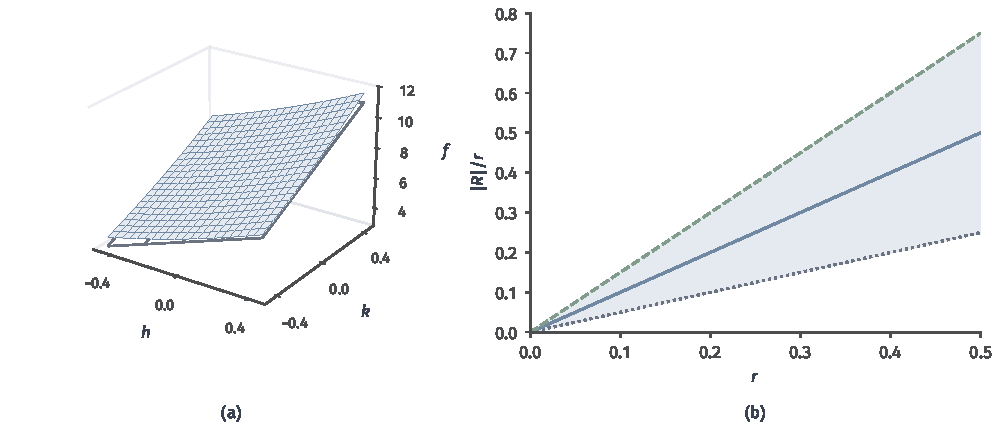
\includegraphics[width=169.0mm]{figures/00-shared/mathematical-preliminaries-upper/00-shared/matplotlib/chapter3-concept-processes/total-differential-remainder.pdf}
 \caption{(a) 二次函数在$(1,2)$附近，灰网格是切平面$P=7+4h+5k$，蓝面是$f(1+h,2+k)$。(b) 令$r=\sqrt{h^2+k^2}$，余项$R=h^2+hk+k^2$满足$r/2\leq R/r\leq3r/2$；阴影给出所有方向的完整范围，三条线是其中的代表值。共同上界随$r\to0$趋零，才保证任意方向都适用同一个线性近似。}
 \label{fig:analysis-process-total-differential-remainder}
\end{figure*}

\paragraph{偏导数连续给出的充分条件}
按定义验证可微需要估计余项，通常不方便。另一种判别只检查偏导数：如果各坐标的变化率在基点附近连续变化，就可以沿坐标逐段走，用它们共同控制全部坐标增量。
与定理~\ref{thm:multivariable-differentiable-necessary}不同，这是一个充分条件，直接保证全微分存在。
\begin{theorem}[偏导数连续与可微性]
\label{thm:multivariable-continuous-partials-sufficient}
设$f:U\to\mathbb R$，$U$开，$\bm a\in U$。若各一阶偏导数在$\bm a$的某个邻域内存在，并在$\bm a$处连续，则$f$在$\bm a$处可微。
\end{theorem}
\begin{proof}
先看$d=2$。从$(a_1,a_2)$走到$(a_1+h_1,a_2+h_2)$，可以先竖直走、再水平走：
\[
 \begin{aligned}
 &f(a_1+h_1,a_2+h_2)-f(a_1,a_2)\\
 &=\bigl[f(a_1+h_1,a_2+h_2)-f(a_1,a_2+h_2)\bigr]\\
 &\quad+\bigl[f(a_1,a_2+h_2)-f(a_1,a_2)\bigr].
 \end{aligned}
\]
第一个方括号只改变第一个坐标，对一元函数$s\mapsto f(s,a_2+h_2)$用中值定理，得到它等于$\partial_1f(\bm\xi_1)h_1$，其中$\bm\xi_1$在这段水平线段上；第二个方括号同理等于$\partial_2f(\bm\xi_2)h_2$，$\bm\xi_2$在竖直线段上。这里用到$\bm h$足够小时两段都在偏导数存在的邻域内。

一般的$d$同样把$\bm a$到$\bm a+\bm h$的增量拆成$d$段，每段只改一个坐标，一元中值定理将第$j$段增量写成$\partial_jf(\bm\xi_j)h_j$，$\bm\xi_j$是第$j$段上的中间点。
减去候选线性项后，误差为$\sum_j\bigl(\partial_jf(\bm\xi_j)-\partial_jf(\bm a)\bigr)h_j$，因此
\[
 \begin{aligned}
 &\left|f(\bm a+\bm h)-f(\bm a)-\sum_{j=1}^d\partial_j f(\bm a)h_j\right|\\
 &\qquad\leq \max_j\left|\partial_j f(\bm\xi_j)-\partial_j f(\bm a)\right|
       \sum_{j=1}^d|h_j|
 =o(\lVert\bm h\rVert_2).
 \end{aligned}
\]
最后一步有两个依据：当$\bm h\to\bm0$时，所有中间点到$\bm a$的距离都不超过$\lVert\bm h\rVert_2$，偏导数在$\bm a$处连续，使最大值一项趋于零；另一方面$\sum_j|h_j|\leq\sqrt d\lVert\bm h\rVert_2$。
这样，各坐标方向上的变化就拼成了同一个有效的全微分。
\end{proof}
偏导数连续只是充分条件：可微只要求函数增量有统一的一阶近似，不要求这些系数随基点连续变化。实际计算中，若各偏导数在所论开集上由连续的表达式给出，就可以直接断定可微。多项式、分母非零的有理函数，以及它们与指数、正弦等连续函数的复合，都属于这种情形。

\paragraph{连续可微函数}
若要求全微分的系数在一个范围内随基点连续变化，就得到连续可微的概念。
实值函数的各一阶偏导数在开集$U$上存在且连续时，称它在$U$上连续可微，记为$C^1(U)$；$C^k(U)$表示直至$k$阶的各偏导数都存在且连续。
定理~\ref{thm:multivariable-continuous-partials-sufficient}保证$C^1$函数处处可微。逆向并不成立，一元函数就足以说明这一点。
\begin{example}[处处可微而导数无界]
\label{ex:multivariable-differentiable-not-c1}
在实轴上令$r(0)=0$，$x\neq0$时令$r(x)=x^2\sin(1/x^2)$。
由于$|r(h)/h|=|h\sin(1/h^2)|\leq|h|\to0$，有$r'(0)=0$；非零点按运算法则求导，得到
\[
 r'(x)=2x\sin(1/x^2)-\frac{2}{x}\cos(1/x^2).
\]
取$x_n=(2\pi n)^{-1/2}$，则$1/x_n^2=2\pi n$，$\sin$项为$0$、$\cos$项为$1$，于是$r'(x_n)=-2/x_n\to-\infty$。所以$r$处处可微，$r'$却在$0$附近无界，在$0$处不连续。
直观上，$r$的振幅被$x^2$压到零，图像在原点与横轴相切；但振荡越来越快，切线斜率剧烈摆动。
在多元情形令$f(\bm x)=r(x_1)$，就得到处处可微而非连续可微的标量函数。
\end{example}

这个例子还说明可微不保证局部Lipschitz连续（定义~\ref{def:ls-lipschitz}）。若$r$在原点的某个邻域内以$L$为Lipschitz常数，该邻域内每个差商的绝对值都不超过$L$，各点导数也就满足$|r'|\leq L$，与$r'(x_n)\to-\infty$矛盾。

\paragraph{必要条件不能反推可微}
可微蕴含连续、偏导数存在和全部双侧方向导数存在。一元函数在一点的导数存在就等价于可微，因为实轴上只有一条直线可走。多元函数还须协调无穷多个输入方向以及弯曲的趋近路径，所以这些必要条件单独或合起来都不能保证可微。下面依次检查它们的逆向。

\paragraph{偏导数存在不保证可微}
坐标偏导数只约束两条坐标切片，并未控制其余方向或路径。
\begin{example}[偏导数存在但不可微]
\label{ex:analysis-partials-not-differentiable}
定义$f:\mathbb{R}^2\to\mathbb{R}$为
\[
 f(x,y)=
 \begin{cases}
  \dfrac{xy}{\sqrt{x^2+y^2}}, & (x,y)\neq(0,0),\\[6pt]
  0, & (x,y)=(0,0).
 \end{cases}
\]
沿两条坐标轴，函数恒为$0$，所以$\partial f/\partial x(0,0)=\partial f/\partial y(0,0)=0$。若$f$在原点可微，由定理~\ref{thm:multivariable-differentiable-necessary}，候选线性部分只能是零映射。可是沿$\bm{h}=(t,t)$，
\[
 \frac{|f(t,t)-f(0,0)|}{\lVert(t,t)\rVert_2}
 =\frac{|t|/\sqrt{2}}{\sqrt{2}|t|}
 =\frac12,
\]
余项与$\lVert\bm{h}\rVert_2$之比不趋于零，故$f$在原点不可微。

用极坐标可以看清曲面的形状：$f=r\cos\theta\sin\theta=\tfrac r2\sin2\theta$。沿每条从原点出发的射线，函数随$r$线性增长，斜率$\tfrac12\sin2\theta$随方向变化。曲面由这些射线组成，像一个起伏的锥面；把它放大任意倍数后形状不变，永远不会变得像一张平面。

沿每个方向$\bm v=(a,b)$，只令$t\downarrow0$的正向方向导数都存在，等于$ab/\sqrt{a^2+b^2}$（零方向取$0$），但它不是关于$\bm v$的线性函数。$t<0$时差商变号，因此$ab\neq0$时双侧方向导数不存在。
最后，由$|xy|/\sqrt{x^2+y^2}\leq\sqrt{x^2+y^2}/2$，$f$在原点连续。
\end{example}

偏导数只看坐标轴，遗漏了其他接近方向；可微则要求曲面放大后接近平面，本例的锥面做不到。本例还说明，即使偏导数存在、全部正向方向导数存在、函数又连续，也推不出可微。这里的正向方向导数是单侧极限，与本节采用的双侧定义不同，使用时要分清。

\paragraph{全部方向导数存在不保证可微}
把坐标切片换成所有固定直线，仍有两件事需要检查：这些变化率能否组成一个线性映射，以及是否有统一的余项控制。先看缺少线性性的情形。
\begin{example}[方向导数不构成线性映射]
\label{ex:multivariable-nonlinear-directional-derivatives}
在非原点处令$p(x,y)=x^3/(x^2+y^2)$，并令$p(0,0)=0$。
沿$\bm v=(a,b)\neq\bm0$，差商为$p(ta,tb)/t=a^3/(a^2+b^2)$，不依赖$t$，所以双侧方向导数存在且$D_{\bm v}p(0,0)=a^3/(a^2+b^2)$。
取坐标方向得到两个偏导数$1$与$0$。若$p$可微，由定理~\ref{thm:multivariable-differentiable-necessary}，沿$(1,1)^\top$的方向导数应为$1\cdot1+0\cdot1=1$，实际却是$1/(1+1)=1/2$。这些方向变化率无法拼成一个线性映射，所以$p$在原点不可微。
\end{example}

示例~\ref{ex:analysis-partials-not-differentiable}只有单侧方向导数；这里的双侧方向导数全部存在，失败只来自线性性。
即使方向导数全部存在并组成一个线性映射，还要检查余项能否统一控制。
\begin{example}[方向导数全为零仍不可微]
\label{ex:multivariable-linear-directionals-not-differentiable}
在非原点处令$q(x,y)=x^3y/(x^4+y^2)$，并令$q(0,0)=0$。
由$2|x^2y|\leq x^4+y^2$，有$|q(x,y)|\leq|x|/2$，故$q$在原点连续。
对固定方向$(a,b)^\top$，若$b\neq0$，
\[
 \frac{q(ta,tb)}t=\frac{t a^3b}{t^2a^4+b^2}\longrightarrow0;
\]
若$b=0$，差商恒为零。因此所有双侧方向导数都为零，它们组成零线性映射。
可是沿$\bm h=(t,t^2)^\top$，$q(t,t^2)=t^5/(2t^4)=t/2$，从而
\[
 \frac{|q(t,t^2)|}{\lVert(t,t^2)\rVert_2}
 =\frac1{2\sqrt{1+t^2}}\longrightarrow\frac12.
\]
候选零映射不满足全微分的余项条件，$q$在原点不可微。
\end{example}

这与示例~\ref{ex:multivariable-parabola-path-limit}中$g$的情形相同：函数沿抛物线有一道坡，每条直线进入原点时都避开了它。方向导数先固定方向再取极限；全微分则要求方向随扰动改变时，误差仍受同一个控制。

\paragraph{连续与偏导数存在互不蕴含}
连续性也推不出微分条件。
例如$f(x,y)=|x|$在整个平面上Lipschitz连续，图像沿$y$轴有一道折痕。原点关于$x$的双侧偏导数不存在，因此$f$在那里不可微。
偏导数存在同样推不出连续：示例~\ref{ex:multivariable-path-limits}中原点置零的$xy/(x^2+y^2)$沿坐标轴恒为零，两个偏导数存在，但它在原点不连续。
所以连续与偏导数存在互不蕴含，可微则同时保证二者。

\paragraph{条件之间的蕴含关系}
把必要条件、充分判别与上面的反例放在一起，得到下面的蕴含链：
\[
 \begin{gathered}
 f\text{在}\bm a\text{的某邻域内连续可微}
 \ \Longrightarrow\ f\text{在}\bm a\text{处可微},\\
 f\text{在}\bm a\text{处可微}
 \ \Longrightarrow\ \text{全部双侧方向导数存在}
 \ \Longrightarrow\ \text{全部偏导数存在}.
 \end{gathered}
\]
第一条由定理~\ref{thm:multivariable-continuous-partials-sufficient}得到，第二条由定理~\ref{thm:multivariable-differentiable-necessary}得到，最后一条只须在全部方向中取坐标方向$\bm e_j$。
同一定理还说明，可微蕴含连续，并且方向导数关于方向是线性映射$\bm v\mapsto\mathrm df_{\bm a}(\bm v)$。
第一行的前提涉及$\bm a$的整个邻域，其余条件只涉及基点$\bm a$本身；链中的方向导数都按双侧极限理解。

各箭头都不能反向：示例~\ref{ex:multivariable-differentiable-not-c1}说明处处可微仍可能不连续可微；示例~\ref{ex:multivariable-nonlinear-directional-derivatives}与示例~\ref{ex:multivariable-linear-directionals-not-differentiable}说明全部双侧方向导数存在仍可能不可微，后者连函数连续、方向导数组成线性映射这两点也都满足；示例~\ref{ex:analysis-partials-not-differentiable}说明偏导数存在不推出全部双侧方向导数存在。不满足偏导数连续这一充分条件时，应回到全微分的定义检查余项。

\subsection{微分的运算法则}
\label{sec:multivariable-differential-rules}

直接按定义求全微分很繁琐。与一元情形一样，可以从简单函数的微分出发，用运算法则组合出复杂函数的微分。
本小节的$f,g$都在同一开集内定义，并在基点$\bm a$处可微，$c$为固定实数。
各法则的证明方法相同：代入各自的一阶展开，整理出关于$\bm h$的线性项，再确认剩下的部分仍是$o(\lVert\bm h\rVert_2)$。这样既证明新函数可微，也读出了它的全微分。

\paragraph{和、差与数乘的微分}
把两个一阶展开相加，
\[
 (f+g)(\bm a+\bm h)=(f+g)(\bm a)+\bigl(\mathrm df_{\bm a}+\mathrm dg_{\bm a}\bigr)(\bm h)+o(\lVert\bm h\rVert_2),
\]
两个线性映射之和仍是线性映射，两个$o(\lVert\bm h\rVert_2)$余项之和仍是$o(\lVert\bm h\rVert_2)$，因此
$\mathrm d(f+g)=\mathrm df+\mathrm dg$。
把加号换成减号，同样的论证给出$\mathrm d(f-g)=\mathrm df-\mathrm dg$。固定系数$c$只会缩放线性项与余项，故$\mathrm d(cf)=c\,\mathrm df$，包括$c=0$的常函数情形。

\paragraph{积的微分}
记$R_f,R_g$为两个一阶展开的余项，都是$o(\lVert\bm h\rVert_2)$。相乘得
\[
 \begin{aligned}
 f(\bm a+\bm h)g(\bm a+\bm h)
 &=\bigl(f(\bm a)+\mathrm df(\bm h)+R_f\bigr)\bigl(g(\bm a)+\mathrm dg(\bm h)+R_g\bigr)\\
 &=f(\bm a)g(\bm a)+g(\bm a)\,\mathrm df(\bm h)+f(\bm a)\,\mathrm dg(\bm h)+(\text{其余各项}).
 \end{aligned}
\]
其余各项要么含有余项$R_f,R_g$乘以有界量，要么是两个线性增量的乘积$\mathrm df(\bm h)\,\mathrm dg(\bm h)=O(\lVert\bm h\rVert_2^2)$，都是$o(\lVert\bm h\rVert_2)$。因此乘积可微，且
\[
 \mathrm d(fg)=g(\bm a)\,\mathrm df+f(\bm a)\,\mathrm dg.
\]
这与一元的$(fg)'=f'g+fg'$形式相同：两个因子各自变化，一阶上贡献可以相加，两个变化同时发生的部分是高阶小量。

\paragraph{商的微分}
设$g(\bm a)\neq0$。可微蕴含连续，所以$g$在$\bm a$附近远离零，$1/g$在$\bm a$附近有定义。记$\delta=g(\bm a+\bm h)-g(\bm a)=\mathrm dg(\bm h)+o(\lVert\bm h\rVert_2)$，它是$O(\lVert\bm h\rVert_2)$。一元函数$1/y$在$g(\bm a)$处的展开给出
\[
 \frac1{g(\bm a)+\delta}=\frac1{g(\bm a)}-\frac{\delta}{g(\bm a)^2}+O(\delta^2).
\]
代入$\delta$的展开，并注意$O(\delta^2)=O(\lVert\bm h\rVert_2^2)$，得到$\mathrm d(1/g)=-\mathrm dg/g(\bm a)^2$。再把$f/g$看成$f\cdot(1/g)$，用积的微分得到
\[
 \mathrm d(f/g)=\frac{g(\bm a)\,\mathrm df-f(\bm a)\,\mathrm dg}{g(\bm a)^2}.
\]
这里分母非零既是定义商函数的条件，也是估计余项的条件。

\paragraph{标量复合函数的微分}
若一元函数$\psi$在$f(\bm a)$处可微，且复合在$\bm a$的邻域内有定义，则$\psi\circ f$在$\bm a$处可微，并且
\[
 \mathrm d(\psi\circ f)=\psi'(f(\bm a))\,\mathrm df.
\]
推导时把内层增量$\delta=f(\bm a+\bm h)-f(\bm a)$代入外层的一元展开$\psi(f(\bm a)+\delta)=\psi(f(\bm a))+\psi'(f(\bm a))\delta+o(|\delta|)$，再把$\delta=\mathrm df(\bm h)+o(\lVert\bm h\rVert_2)$代入。
因为$\delta=O(\lVert\bm h\rVert_2)$，外层余项$o(|\delta|)$仍是$o(\lVert\bm h\rVert_2)$。
例如$-(x^2+y^2)$在$(x,y)$处的全微分为$(h,k)\mapsto-2xh-2yk$，所以$e^{-(x^2+y^2)}$的全微分是$(h,k)\mapsto e^{-(x^2+y^2)}(-2xh-2yk)$：外层只把内层的全微分乘上一个正数。

\paragraph{沿参数曲线的变化率}
外层也可以是多元函数、内层是一元的参数曲线。设$\bm x:I\to U$定义在开区间$I$上，各坐标在$t_0$处可微，记速度向量$\bm x'(t_0)=(x_1'(t_0),\ldots,x_d'(t_0))^\top$；又设$f$在$\bm a=\bm x(t_0)$处可微。则$t\mapsto f(\bm x(t))$在$t_0$处可微，且
\begin{equation}
 \frac{\mathrm d}{\mathrm dt}f(\bm x(t))\Big|_{t=t_0}
 =\mathrm df_{\bm a}\bigl(\bm x'(t_0)\bigr)
 =\sum_{j=1}^d\partial_jf(\bm a)\,x_j'(t_0).
\label{eq:multivariable-curve-chain-rule}
\end{equation}
推导与上一段相同。记内层增量$\bm k=\bm x(t_0+s)-\bm x(t_0)$，各坐标的一元展开给出$\bm k=s\bm x'(t_0)+o(|s|)$，因而$\lVert\bm k\rVert_2=O(|s|)$。代入$f$的一阶展开，
\[
 f(\bm x(t_0+s))-f(\bm a)=\mathrm df_{\bm a}(\bm k)+o(\lVert\bm k\rVert_2)
 =s\,\mathrm df_{\bm a}(\bm x'(t_0))+o(|s|),
\]
第二步用了全微分的线性，以及线性映射把长度为$o(|s|)$的向量仍变成$o(|s|)$的数。除以$s$并令$s\to0$即得。
内层的变化先在输入空间中产生速度向量$\bm x'(t_0)$，外层的全微分再作用于这个方向。取直线$\bm x(t)=\bm a+t\bm v$，便回到方向导数公式$D_{\bm v}f(\bm a)=\mathrm df_{\bm a}(\bm v)$。下一小节用式~\eqref{eq:multivariable-curve-chain-rule}说明梯度与等值曲线的切向正交；一般向量值映射的复合在第~\ref{sec:analysis-vector-chain-matrix-calculus}节处理。

\paragraph{二次型的微分}
二次型是向量自变量的标量函数，平方误差、能量函数等都含有这种结构。考虑$q(\bm{x})=\bm{x}^{\top}\bm{A}\bm{x}=\sum_{i,j}A_{i,j}x_ix_j$，其中$\bm{A}\in\mathbb{R}^{d\times d}$固定。它是有限个乘积的和，可以直接用乘积法则：把两个$\bm x$看成两个因子，每次只让一个变化，
\begin{align*}
  \mathrm{d}q_{\bm x}(\bm h)
  &=
  \bm h^{\top}\bm{A}\bm{x}
  +\bm{x}^{\top}\bm{A}\bm h\\
  &=
  \bm{x}^{\top}(\bm{A}^{\top}+\bm{A})\bm h.
\end{align*}
第二步用到$\bm h^\top\bm A\bm x$是一个实数，等于自己的转置$\bm x^\top\bm A^\top\bm h$。所以全微分的系数，即各偏导数排成的列向量，为
\begin{equation}
  \bigl(\partial_1q(\bm x),\ldots,\partial_dq(\bm x)\bigr)^\top
  =
  (\bm{A}+\bm{A}^{\top})\bm{x}.
\label{eq:analysis-quadratic-form-gradient}
\end{equation}
当$\bm{A}$对称时，式~\eqref{eq:analysis-quadratic-form-gradient}化为$2\bm{A}\bm{x}$，与一元的$(ax^2)'=2ax$对应。$\bm A$不对称时不能写成$2\bm{A}\bm{x}$，否则就默认了对称性。
例如
\[
 \bm A=\begin{bmatrix}0&1\\0&0\end{bmatrix}
\]
时$q=x_1x_2$，直接求偏导得$(x_2,x_1)^\top$，与$(\bm A+\bm A^\top)\bm x$一致；而$2\bm A\bm x=(2x_2,0)^\top$是错的。

\paragraph{二次型的精确增量}
乘积法则只给出一阶项。对二次型还可以直接写出完整增量，把一阶项与实际误差放在同一个式子里。设$\bm S$对称，展开得
\[
 q(\bm x+\bm h)-q(\bm x)
 =\bm h^\top\bm S\bm x+\bm x^\top\bm S\bm h+\bm h^\top\bm S\bm h
 =2\bm x^\top\bm S\bm h+\bm h^\top\bm S\bm h,
\]
其中用到$\bm h^\top\bm S\bm x=(\bm h^\top\bm S\bm x)^\top=\bm x^\top\bm S\bm h$。由Cauchy--Schwarz不等式与谱范数的定义（第~\ref{sec:multivariable-operator-norm}节），
\[
 |\bm h^\top\bm S\bm h|\leq\lVert\bm h\rVert_2\lVert\bm S\bm h\rVert_2\leq\lVert\bm S\rVert_2\lVert\bm h\rVert_2^2 .
\]
所以余项不只是$o(\lVert\bm h\rVert_2)$，而是被一个明确的二次量控制；这也独立地证明了$q$可微，且$\mathrm dq_{\bm x}(\bm h)=2\bm x^\top\bm S\bm h$。
例如$x^2+xy+y^2=\bm x^\top\bm S\bm x$，其中
\[
 \bm S=\begin{bmatrix}1&1/2\\1/2&1\end{bmatrix}
\]
的特征值为$3/2$与$1/2$。对称矩阵的谱范数是特征值绝对值的最大者（第~\ref{chap:eigen-spectral-decomposition}章），故$\lVert\bm S\rVert_2=3/2$，这正是示例~\ref{ex:multivariable-quadratic-differential}中余项上界$\tfrac32(h^2+k^2)$的常数。
二次项$\bm h^\top\bm S\bm h$在第~\ref{sec:multivariable-curvature-error}节成为Hessian二次型，梯度和余项估计也将复用这个例子。

\subsection{梯度与内积}
\label{sec:multivariable-gradient-inner-product}

可微时，全微分$\mathrm df_{\bm a}$是$\mathbb R^d$上的线性泛函，即对偶空间中的元素（第~\ref{sec:ls-dual-spaces}节）：它读取一个输入扰动，给出函数值的一阶变化。泛函本身不是输入空间中的向量，不能画成地图上的箭头。第~\ref{sec:ls-riesz-representation}节的Riesz表示定理说明，选定内积后，每个线性泛函都等于与唯一一个向量的内积。把这个向量作为全微分的表示，就得到梯度。
\begin{definition}[梯度]
\label{def:multivariable-gradient}
设$\mathbb R^d$上取定内积$\langle\cdot,\cdot\rangle$，$f:U\to\mathbb R$在$\bm a$处可微。满足
\[
 \mathrm df_{\bm a}(\bm h)=\langle\nabla f(\bm a),\bm h\rangle\qquad(\bm h\in\mathbb R^d)
\]
的唯一向量$\nabla f(\bm a)\in\mathbb R^d$称为$f$在$\bm a$处的\term{梯度}（gradient）。未加说明时取标准欧氏内积$\langle\bm x,\bm y\rangle=\bm x^\top\bm y$。
\end{definition}
在标准欧氏内积下，比较定理~\ref{thm:multivariable-differentiable-necessary}中的$\mathrm df_{\bm a}(\bm h)=\sum_j\partial_jf(\bm a)h_j$与$\nabla f(\bm a)^\top\bm h$，逐个取$\bm h=\bm e_j$，得到
\begin{equation}
 \nabla f(\bm a)=\bigl(\partial_1f(\bm a),\ldots,\partial_df(\bm a)\bigr)^\top .
\label{eq:multivariable-gradient-coordinates}
\end{equation}
于是可微函数满足$f(\bm a+\bm h)=f(\bm a)+\nabla f(\bm a)^\top\bm h+o(\lVert\bm h\rVert_2)$，方向导数为$D_{\bm v}f(\bm a)=\nabla f(\bm a)^\top\bm v$。
例如$f(x,y)=x^2+xy+y^2$的梯度为$\nabla f(x,y)=(2x+y,x+2y)^\top$，$\nabla f(1,2)=(4,5)^\top$；由式~\eqref{eq:analysis-quadratic-form-gradient}，一般二次型有$\nabla_{\bm x}(\bm x^\top\bm A\bm x)=(\bm A+\bm A^\top)\bm x$。
梯度与输入属于同一个空间：$(4,5)^\top$可以画成地图平面上从$(1,2)$出发的一支箭头，而不是曲面上的向量。

若$f$在开集$U$上处处可微，把每一点的梯度放在该点，就得到$U$上的向量场$\nabla f:U\to\mathbb R^d$，称为$f$的梯度场。例如第~\ref{sec:multivariable-scalar-fields}节的标量场$x^2+y^2$的梯度场是$(2x,2y)^\top$，箭头从原点向外，离原点越远越长，与那里观察到的“等值圆越来越密”相符。哪些向量场是某个标量场的梯度场，留到第~\ref{sec:multivariable-potential-path-independence}节研究。

表示向量随泛函线性变化，所以上一小节的法则直接改写为梯度的法则：$\nabla(f\pm g)=\nabla f\pm\nabla g$，$\nabla(cf)=c\nabla f$，$\nabla(fg)=g(\bm a)\nabla f+f(\bm a)\nabla g$，$\nabla(\psi\circ f)=\psi'(f(\bm a))\nabla f$。例如$\nabla e^{-(x^2+y^2)}=e^{-(x^2+y^2)}(-2x,-2y)^\top$，与$-(x^2+y^2)$的梯度同向，都指向原点。

\paragraph{偏导数向量与梯度}
式~\eqref{eq:multivariable-gradient-coordinates}的右侧在偏导数全部存在时就能写出，本书在这种情形下也用记号$\nabla f(\bm a)$表示这一列偏导数。但第~\ref{sec:multivariable-total-differentiation}节的反例说明，这时它只是坐标变化率排成的向量：示例~\ref{ex:multivariable-nonlinear-directional-derivatives}中这一列是$(1,0)^\top$，却给不出沿$(1,1)^\top$的方向导数。只有确认可微以后，它才代表对所有方向同时有效的一阶近似，才可以用内积计算任意方向导数，并解释为最快上升的方向。

梯度的列向量排列也来自所选内积和坐标：全微分本身是一个线性作用，标准欧氏内积把它的系数原样排成列向量。换用其他内积时，同一个全微分由另一个向量表示。

\paragraph{改变内积时的梯度}
设$\mathbb R^d$上的内积在标准坐标下写成$\langle\bm x,\bm y\rangle_{\bm G}=\bm x^\top\bm G\bm y$，其中$\bm G$对称正定。第~\ref{sec:ls-gram-coordinates}节说明，任何内积在坐标下都是这种形式，$\bm G$就是基的Gram矩阵。记全微分的系数向量为$\bm c=\bigl(\partial_jf(\bm a)\bigr)_{j=1}^d$。要求$\mathrm df_{\bm a}(\bm h)=\bm c^\top\bm h=\bm g^\top\bm G\bm h$对所有$\bm h$成立，等价于$\bm G\bm g=\bm c$，所以
\begin{equation}
 \nabla_{\bm G}f(\bm a)=\bm G^{-1}\bigl(\partial_jf(\bm a)\bigr)_{j=1}^d .
\label{eq:multivariable-gradient-gram}
\end{equation}
系数向量$\bm c$由函数本身决定；改变的只是用哪个向量来表示同一个全微分。
\begin{example}[加权内积下的梯度]
\label{ex:multivariable-weighted-gradient}
仍取$f(x,y)=x^2+xy+y^2$与基点$(1,2)$，系数向量为$(4,5)^\top$。改用$\bm G=\operatorname{diag}(4,1)$给出的加权内积$\langle\bm x,\bm y\rangle_{\bm G}=4x_1y_1+x_2y_2$，由式~\eqref{eq:multivariable-gradient-gram}，
\[
 \nabla_{\bm G}f(1,2)=\operatorname{diag}(1/4,1)\,(4,5)^\top=(1,5)^\top.
\]
核对：$\langle(1,5)^\top,(h,k)^\top\rangle_{\bm G}=4h+5k$，正是同一个全微分。欧氏梯度$(4,5)^\top$与加权梯度$(1,5)^\top$方向不同：加权长度把第一坐标的位移计为原来的两倍，沿它走同样的加权距离只需更小的坐标位移。
\end{example}
这与第~\ref{sec:ls-riesz-representation}节的结论一致：读取本身不变，表示向量随内积改变。

\paragraph{最陡上升方向}
设$f$在$\bm a$处可微，$\bm u$满足$\lVert\bm u\rVert=1$，这里的长度由所选内积诱导。由Cauchy--Schwarz不等式（定理~\ref{thm:linear-algebra-cauchy-schwarz}），
\[
 D_{\bm u}f(\bm a)=\langle\nabla f(\bm a),\bm u\rangle\leq\lVert\nabla f(\bm a)\rVert.
\]
梯度非零时，取$\bm u=\nabla f(\bm a)/\lVert\nabla f(\bm a)\rVert$即达到等号。所以在所选内积的单位长度约束下，梯度方向是局部上升最快的方向，最大坡度等于梯度的长度；反方向$-\nabla f(\bm a)$则下降最快。
示例~\ref{ex:multivariable-weighted-gradient}中，欧氏单位长度下最快方向沿$(4,5)^\top$，加权单位长度下则沿$(1,5)^\top$。“最快”总是相对某种长度而言的。

\paragraph{梯度与等值曲线}
若$\bm u$与梯度正交，方向导数为零，函数值一阶上不变。设$\bm x:I\to U$是一条落在等值集$\{\bm y:f(\bm y)=f(\bm a)\}$中的可微曲线，$\bm x(t_0)=\bm a$。$f(\bm x(t))$恒为常数，由式~\eqref{eq:multivariable-curve-chain-rule}，
\[
 0=\frac{\mathrm d}{\mathrm dt}f(\bm x(t))\Big|_{t=t_0}=\langle\nabla f(\bm a),\bm x'(t_0)\rangle,
\]
所以梯度与这条曲线的切向量正交。这里假定了等值集中确有经过$\bm a$的可微曲线；整个等值集在$\bm a$附近是否为光滑曲线或曲面，还需要第~\ref{sec:analysis-implicit-parameter-integral}章的隐函数定理及梯度非零这一非退化条件。梯度为零只说明一阶项消失，函数在该点附近怎样变化，要由第~\ref{sec:multivariable-curvature-error}节的高阶微分继续判断。

图~\ref{fig:analysis-process-gradient-level-curves}用同一个二次函数比较梯度方向、等值曲线切向及另一个单位方向。
\begin{figure}[!htbp]
 \centering
 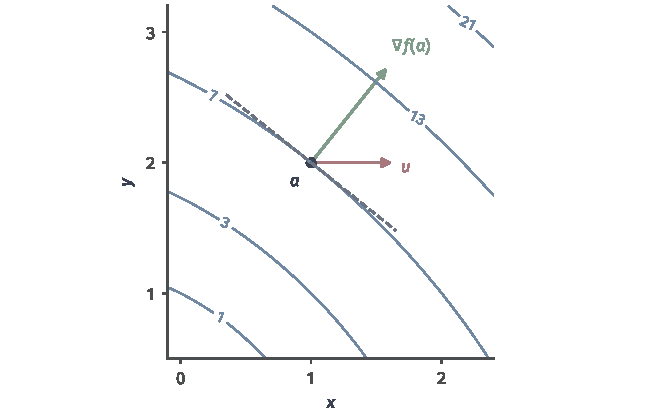
\includegraphics[width=112.0mm]{figures/00-shared/mathematical-preliminaries-upper/00-shared/matplotlib/chapter3-concept-processes/gradient-level-curves.pdf}
 \caption{$f=x^2+xy+y^2$的等值曲线，标注为函数值；基点$a=(1,2)$处$\nabla f=(4,5)^\top$，图中绿箭头按$0.15$倍绘制。灰虚线沿$(5,-4)^\top$，与梯度垂直，因而与经过$a$的等值曲线相切；红箭头为$u=(1,0)^\top$。比较最快上升方向时须先归一化，不能直接比较图中箭头长度。}
 \label{fig:analysis-process-gradient-level-curves}
\end{figure}

\subsection{中值估计与局部Lipschitz性}
\label{sec:multivariable-scalar-mean-value-lipschitz}

微分描述一点附近的变化。要估计两点之间的有限变化，可以沿连接两点的线段把函数限制为一元函数，再使用一元中值定理。前提是整条线段都在定义域内。
记$[\bm x,\bm y]=\{\bm x+t(\bm y-\bm x):0\leq t\leq1\}$为连接两点的线段。
\begin{theorem}[多元标量函数的中值公式]
\label{thm:multivariable-scalar-mean-value}
设$f$在包含$[\bm x,\bm y]$的开集上可微，$\bm x\neq\bm y$。则存在$\theta\in(0,1)$使
\[
 f(\bm y)-f(\bm x)=\nabla f(\bm x+\theta(\bm y-\bm x))^\top(\bm y-\bm x).
\]
\end{theorem}
\begin{proof}
令$\phi(t)=f(\bm x+t(\bm y-\bm x))$，$t\in[0,1]$，它是$f$在线段上的一元切片。$\phi'(t)$就是$f$在点$\bm x+t(\bm y-\bm x)$处沿$\bm y-\bm x$的方向导数，所以$\phi'(t)=\nabla f(\bm x+t(\bm y-\bm x))^\top(\bm y-\bm x)$。
对$\phi$在$[0,1]$上使用一元中值定理，$\phi(1)-\phi(0)=\phi'(\theta)$，这就是所述等式。
\end{proof}
等式说明，两点之间的平均变化率等于线段上某一点沿该方向的瞬时变化率。这是一元“平均斜率等于某点切线斜率”的直接推广。
例如$f(x,y)=x^2+y^2$，$\bm x=(0,0)$、$\bm y=(1,1)$，左侧为$2$；右侧为$\nabla f(\theta,\theta)^\top(1,1)^\top=4\theta$，取$\theta=1/2$即相等，中值点恰为线段中点。

\paragraph{局部Lipschitz性}
\phantomsection
\label{def:multivariable-lipschitz}
定义~\ref{def:ls-lipschitz}已经给出Lipschitz连续与局部Lipschitz连续：存在常数$L$，使输出距离不超过输入距离的$L$倍，局部情形允许常数随邻域改变。那里只说明了这种误差控制的含义，本小节的新任务是由导数求出这样的常数。

中值公式把有限增量写成某点梯度与位移的内积；若梯度的长度有统一上界，就能用输入距离的常数倍控制输出变化。以下距离都取欧氏范数。优化中常用这种控制由步长估计函数值的变化。

先看两个不依赖导数就能读出常数的例子。线性函数$f(\bm x)=\bm a^\top\bm x$满足$|f(\bm x)-f(\bm y)|=|\bm a^\top(\bm x-\bm y)|\leq\lVert\bm a\rVert_2\lVert\bm x-\bm y\rVert_2$，Lipschitz常数可取$\lVert\bm a\rVert_2$，它恰是梯度的长度。
欧氏范数$f(\bm x)=\lVert\bm x\rVert_2$由三角不等式满足$|\lVert\bm x\rVert_2-\lVert\bm y\rVert_2|\leq\lVert\bm x-\bm y\rVert_2$，常数为$1$，尽管它在原点不可微。所以Lipschitz连续本身不要求处处可微。

要把梯度界转化为Lipschitz常数，两点之间的线段必须留在定义域内。若集合$D$中任意两点之间的线段都含于$D$，就称$D$为凸集。在凸开集上，梯度长度的统一上界恰好就是Lipschitz常数。
\begin{theorem}[梯度有界与Lipschitz条件]
\label{thm:multivariable-gradient-lipschitz}
设$U\subseteq\mathbb R^d$为凸开集，$f:U\to\mathbb R$可微。则$f$在$U$上以$L$为Lipschitz常数，当且仅当$\lVert\nabla f(\bm x)\rVert_2\leq L$对所有$\bm x\in U$成立。
\end{theorem}
\begin{proof}
若梯度长度不超过$L$，任取$\bm x\neq\bm y$，凸性保证线段$[\bm x,\bm y]\subseteq U$。由中值公式与内积不等式，
\[
 |f(\bm y)-f(\bm x)|=\bigl|\nabla f(\bm\xi)^\top(\bm y-\bm x)\bigr|\leq\lVert\nabla f(\bm\xi)\rVert_2\lVert\bm y-\bm x\rVert_2\leq L\lVert\bm y-\bm x\rVert_2.
\]
反过来，设$f$以$L$为Lipschitz常数。固定$\bm x$，若$\nabla f(\bm x)\neq\bm0$，取单位方向$\bm u=\nabla f(\bm x)/\lVert\nabla f(\bm x)\rVert_2$，则
\[
 \lVert\nabla f(\bm x)\rVert_2=D_{\bm u}f(\bm x)=\lim_{t\downarrow0}\frac{f(\bm x+t\bm u)-f(\bm x)}t\leq\lim_{t\downarrow0}\frac{Lt}t=L.
\]
梯度为零时不等式自然成立。
\end{proof}
几何上，若坡度处处不超过$L$，沿直线走过距离$\rho$，高度最多改变$L\rho$；反过来，Lipschitz常数也限制了每一点最陡方向的坡度。
例如$f(x,y)=\sin x+\cos y$满足$\lVert\nabla f\rVert_2=\sqrt{\cos^2x+\sin^2y}\leq\sqrt2$，所以它在整个平面上以$\sqrt2$为Lipschitz常数。

定理中的凸性不能省略。在不凸的区域上，梯度可以处处很小，函数值却在两个很近的点之间相差很大。
\begin{example}[非凸区域上梯度有界而不Lipschitz]
\label{ex:multivariable-nonconvex-lipschitz-failure}
取去掉负$x$轴的环形区域$D=\{1<\lVert\bm x\rVert_2<2\}\setminus\{(x,0):x<0\}$，令$f(\bm x)$为点$\bm x$的极角，取值于$(-\pi,\pi)$。$f$在$D$上可微，$\lVert\nabla f\rVert_2=1/r<1$，坡度处处小于$1$。
但取负$x$轴两侧的点$(-1.5,\pm\varepsilon)$，两点距离为$2\varepsilon$，极角却分别接近$\pi$与$-\pi$，相差接近$2\pi$。令$\varepsilon\to0$，函数值之差与距离之比无界，所以$f$在$D$上不是Lipschitz函数。
\end{example}

连接这两点的直线段穿过被去掉的负$x$轴，不在$D$内，中值公式无法使用。$D$内连接两点的路径必须绕过原点，长度远大于$2\varepsilon$。可见梯度界只能沿含于定义域的线段转化为函数值之差的界。

局部情形不需要整个定义域凸。若$f\in C^1(U)$，在每个基点附近取一个包含在$U$内的闭球。连续函数$\lVert\nabla f\rVert_2$在这个闭有界集上有界（定理~\ref{thm:multivariable-extreme-value}），因而在同心的开球上也有界。开球是凸开集，由定理~\ref{thm:multivariable-gradient-lipschitz}，$f$在这个开球上Lipschitz连续，所以$f$局部Lipschitz连续。
各点的局部常数不一定有共同上界：$f(x,y)=x^2$连续可微，但$\lVert\nabla f\rVert_2=2|x|$在全平面无界，因而它不是全域Lipschitz函数。

\paragraph{三种控制的强弱}
至此出现了三种关于函数变化的结论，强度各不相同。连续只保证$\bm x\to\bm a$时$f(\bm x)\to f(\bm a)$，不给出趋近的速度。可微给出渐近的线性近似：误差是$o(\lVert\bm h\rVert_2)$，但对一个给定的有限步长，它不说明误差有多大。梯度的统一界则沿含于定义域的线段控制有限距离上的变化，常数明确，却只估计变化的大小，不估计线性预测还差多少。

要估计一阶预测还差多少，需要把后两种结论结合起来，考察导数本身沿线段怎样变化。第~\ref{sec:multivariable-curvature-error}节的Taylor公式用二阶导数描述这种变化；只用一阶导数的余项界，以及误差被放大多少倍的局部条件数，集中在第~\ref{chap:differential-perturbation-analysis}章讨论。

\section{多元向量值函数的微分}
\label{sec:multivariable-vector-differentiation}

前面每个输入只产生一个实数。本节研究同时产生$m$个输出分量的映射$F:U\subseteq\mathbb R^d\to\mathbb R^m$，关心输入稍作改变时输出点整体怎样移动。

例如极坐标映射$(r,\theta)\mapsto(r\cos\theta,r\sin\theta)$把两个参数变成平面上的点，神经网络的一层把输入向量变成另一个向量；参数曲线（$d=1$）与参数曲面（$d=2$、$m=3$）也是这种映射。
输出只有有限个分量，所以可以逐个分量使用前面的结论。但每个分量仍要对全部输入方向整体扰动，不能用坐标切片代替各分量的全微分。本节先用一个线性映射定义整体可微并引入Jacobian矩阵，再给出复合映射的导数，最后用导数的算子范数估计有限增量。

\subsection{Jacobian矩阵}

向量值函数由它的全部输出分量确定，因此按分量书写。
\begin{definition}[多元向量值函数]
\label{def:multivariable-vector-function}
映射$F:U\subseteq\mathbb R^d\to\mathbb R^m$称为多元向量值函数，写作$F=(F_1,\ldots,F_m)^\top$，其中每个$F_i:U\to\mathbb R$为多元标量函数。
\end{definition}
向量值函数的极限与连续性已在第~\ref{sec:multivariable-joint-limit-section}节与第~\ref{sec:multivariable-continuity}节定义，第~\ref{sec:multivariable-field-limits-continuity}节回顾了要点：输出点整体接近，等价于每个输出分量接近；每个分量的极限仍是对全部输入方向的联合极限。本节在连续性的基础上进一步研究线性近似。向量场是$m=d$的特例，下面的结论对它同样适用。

\paragraph{微分与Jacobian矩阵}

标量输出的全微分是到实数的线性映射，也称线性泛函。向量输出的全微分则要把输入扰动映射为$m$维输出扰动。
有限维线性映射由矩阵表示，矩阵的每一行记录一个输出分量的系数。
\begin{definition}[向量值函数的微分]
\label{def:multivariable-vector-differential}
设$U$开，$F:U\to\mathbb R^m$，$\bm a\in U$。若存在线性映射$\mathrm dF_{\bm a}:\mathbb R^d\to\mathbb R^m$，记它在标准基下的矩阵为$\bm J_F(\bm a)\in\mathbb R^{m\times d}$，使
\begin{equation}
 F(\bm a+\bm h)=F(\bm a)+\bm J_F(\bm a)\bm h+o(\lVert\bm h\rVert_2),
\label{eq:analysis-jacobian-linearization}
\end{equation}
则称$F$在$\bm a$处可微，余项按输出欧氏范数理解。
$\mathrm dF_{\bm a}(\bm h)=\bm J_F(\bm a)\bm h$称为$F$在$\bm a$处的微分，矩阵$\bm J_F(\bm a)$称为\term{Jacobian矩阵}（Jacobian matrix）。
\end{definition}
向量值函数可微当且仅当每个输出分量$F_i$可微。正向只需从向量余项取第$i$个分量，它的绝对值不超过向量余项的欧氏长度，于是得到$F_i$的标量展开；反向则把有限个分量的$o(\lVert\bm h\rVert_2)$余项用欧氏范数合并，合并后仍是$o(\lVert\bm h\rVert_2)$。
由此，Jacobian的第$i$行是分量梯度的转置$\nabla F_i^\top$，第$i,j$个元素为$\partial_jF_i$；微分若存在则唯一。$C^k$向量值函数指所有输出分量都属于$C^k$。

本书把输入、输出都写成列向量，因此$\bm J_F(\bm a)$是“输出维数$\times$输入维数”的矩阵：第$i$行记录第$i$个输出对各输入的偏导数，$\bm J_F(\bm a)\bm h$的形状为$(m\times d)(d\times1)=m\times1$，与输出一致。$m=1$时Jacobian是$1\times d$的行向量$\nabla f(\bm a)^\top$，梯度则是列向量，二者互为转置。

\paragraph{Jacobian矩阵的几何意义}
按行看，Jacobian记录各输出分量的梯度；按列看，它记录各输入坐标对输出点的推动。第$j$列
\[
 \bm J_F(\bm a)\bm e_j=(\partial_jF_1,\ldots,\partial_jF_m)^\top
\]
表示：只把第$j$个输入增加一个很小的量$t$时，输出点大约移动这个向量的$t$倍。一般扰动$\bm h=\sum_jh_j\bm e_j$的一阶效果，就是这些列按$h_j$加权求和。
对$d=m=2$，由此得到局部伸缩的图像。以$\bm a$为角、边长为$\varepsilon$的小正方形由$\varepsilon\bm e_1,\varepsilon\bm e_2$张成，它的像近似是由$\varepsilon\bm J_F\bm e_1,\varepsilon\bm J_F\bm e_2$张成的平行四边形。行列式的绝对值是线性映射对面积的缩放倍数（第~\ref{sec:prelim-determinants}节），所以像的面积约为$|\det\bm J_F(\bm a)|\varepsilon^2$；行列式的符号说明局部是否翻转了定向。

极坐标映射是这种局部伸缩的一个具体例子。
\begin{example}[极坐标映射的Jacobian矩阵]
\label{ex:multivariable-polar-jacobian}
考虑极坐标映射
\[
 P(r,\theta)=(r\cos\theta,r\sin\theta)^\top.
\]
逐个输出分量求偏导，得到
\[
\begin{gathered}
\bm J_P(r,\theta)=\begin{bmatrix}\cos\theta&-r\sin\theta\\ \sin\theta&r\cos\theta\end{bmatrix}\\
\det\bm J_P=r\cos^2\theta+r\sin^2\theta=r.
\end{gathered}
\]
第一列是单位径向向量：$r$增加$\mathrm dr$，点沿射线向外移动$\mathrm dr$。第二列长度为$r$、沿圆周切向：$\theta$增加$\mathrm d\theta$，点沿半径为$r$的圆移动约$r\,\mathrm d\theta$。因此参数平面中面积为$\mathrm dr\,\mathrm d\theta$的小矩形，变成面积约为$r\,\mathrm dr\,\mathrm d\theta$的小扇形块。
\end{example}

离原点越远，同样的角度增量扫过的弧越长，面积放大越多。第~\ref{sec:classical-change-variables}节的区域积分换元就用这个倍数校正面积。

对一般的非线性映射，小网格块的像是弯边块，线性近似把它换成平行四边形。图~\ref{fig:analysis-process-jacobian-grid-cell}画出了这种对应。图中$\det J_T(a)=1\times0.6-0.25\times0.3=0.525$，所以绿色小方块的像面积约为原面积的一半。
\begin{figure*}[!htbp]
 \centering
 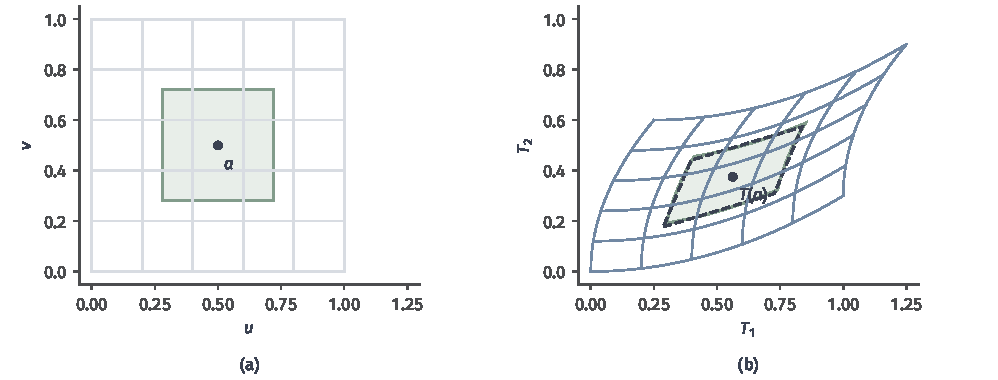
\includegraphics[width=169.0mm]{figures/00-shared/mathematical-preliminaries-upper/00-shared/matplotlib/chapter3-concept-processes/jacobian-grid-cell.pdf}
 \caption{取$T(u,v)=(u+v^2/4,\,0.6v+0.3u^2)$，$a=(0.5,0.5)$。(a) 输入网格及绿色小方块。(b) 非线性像为弯边块，黑虚线为$T(a)+J_T(a)(h,k)^\top$给出的平行四边形；$J_T(a)=\bigl[\begin{smallmatrix}1&0.25\\0.3&0.6\end{smallmatrix}\bigr]$。有限块不与线性像完全重合，缩小扰动后才由可微余项控制差异。}
 \label{fig:analysis-process-jacobian-grid-cell}
\end{figure*}

输入、输出维数不同时，同一个原则给出非方阵的Jacobian。
\begin{example}[空间螺旋线的Jacobian矩阵]
\label{ex:multivariable-helix-jacobian}
令$\bm\gamma(t)=(\cos t,\sin t,t)^\top$，$t\in\mathbb R$，输入一维、输出三维。逐分量求导得
\[
 \bm J_{\bm\gamma}(t)=\begin{bmatrix}-\sin t\\ \cos t\\ 1\end{bmatrix}\in\mathbb R^{3\times1}.
\]
它把参数增量$s$映为$s\bm J_{\bm\gamma}(t)$：点沿速度向量$\bm\gamma'(t)$移动。这一列就是曲线的切向量，长度为$\sqrt2$，说明参数每增加一个单位，点约移动$\sqrt2$的距离。
\end{example}
螺旋线的Jacobian不是方阵，没有行列式可言，局部伸缩由切向量的长度描述。极坐标与螺旋线说明，“微分是线性映射”这一原则在不同输入、输出维数下给出形状不同的矩阵，不能默认Jacobian是方阵或有行列式。梯度映射$\bm x\mapsto\nabla f(\bm x)$本身也是从$\mathbb R^d$到$\mathbb R^d$的向量值映射，第~\ref{sec:multivariable-curvature-error}节将研究它的微分，并由此得到Hessian矩阵。

\paragraph{Jacobian矩阵的计算}
计算Jacobian矩阵时，先把每个输出分量当作标量函数求偏导，再按行排列；排好后核对矩阵形状是否为“输出维数$\times$输入维数”。
例如$F(x,y)=(x^2+xy,y^2)^\top$的Jacobian为
\[
 \bm J_F(x,y)=\begin{bmatrix}2x+y&x\\0&2y\end{bmatrix}.
\]
在$(1,2)$处，它把扰动$(h,k)^\top$的一阶影响写成$(4h+k,4k)^\top$。第一行说明第一个输出同时受两个输入推动，第二行说明第二个输出只随$y$变化；两列分别记录沿$x$、沿$y$移动时输出点的位移方向。

再看机器学习中常用的一个向量值映射。它把任意一组实数变成总和为$1$的正权重：先取指数，再除以共同的总和。
这就是$n$维\term{归一化指数映射}（softmax），分类模型常用它把各类别的得分变成概率。对正整数$n$和
$\bm{z}\in\mathbb{R}^n$，令
\[
 \begin{gathered}
s_i(\bm{z})
  =
  \frac{e^{z_i}}{\sum_{k=1}^n e^{z_k}}\\
i=1,\ldots,n.
 \end{gathered}
\]
记分母为$Z=\sum_k e^{z_k}$，它对$z_j$的偏导数为$e^{z_j}$。对分子$e^{z_i}$求偏导，$i=j$时得$e^{z_i}$，$i\neq j$时得$0$，记为$\mathbb{I}\{i=j\}e^{z_i}$。商法则给出
\[
  \frac{\partial s_i}{\partial z_j}
  =
  \frac{\mathbb{I}\{i=j\}e^{z_i}Z-e^{z_i}e^{z_j}}{Z^2}
  =
  s_i\bigl(\mathbb{I}\{i=j\}-s_j\bigr).
\]
因此整个Jacobian矩阵为
\begin{equation}
  \bm{J}_{\bm{s}}(\bm{z})
  =
  \operatorname{diag}(\bm{s})-\bm{s}\bm{s}^{\top}.
\label{eq:analysis-softmax-jacobian}
\end{equation}
这里$\operatorname{diag}(\bm s)$表示以$s_1,\ldots,s_n$为对角元、其他元素为零的对角矩阵。

当$n\geq2$时，对角项$s_i(1-s_i)$为正，描述提高$z_i$对自身分量的影响。非对角项$-s_is_j$为负，它来自共同分母：提高一个得分会压低其余分量。当$n=1$时输出恒为$1$，Jacobian为零。

每行元素之和为$s_i-s_i\sum_js_j=0$。这与给所有$z_i$加同一常数不改变输出相符：沿方向$(1,\ldots,1)^\top$的一阶变化为零。

在最简单的情形中，可以用数值核对式~\eqref{eq:analysis-softmax-jacobian}给出的线性近似。
\begin{example}[二维softmax的Jacobian矩阵]
\label{ex:multivariable-softmax-jacobian-check}
取$n=2$、$\bm z=\bm 0$，则$\bm s=(1/2,1/2)^\top$，由式~\eqref{eq:analysis-softmax-jacobian}，
\[
 \bm J_{\bm s}(\bm 0)
 =\begin{bmatrix}1/2&0\\0&1/2\end{bmatrix}-\begin{bmatrix}1/4&1/4\\1/4&1/4\end{bmatrix}
 =\begin{bmatrix}1/4&-1/4\\-1/4&1/4\end{bmatrix}.
\]
把$z_1$提高$0.1$，线性近似给出$\bm s$的增量约为
\[
 \bm J_{\bm s}(\bm 0)(0.1,0)^\top=(0.025,-0.025)^\top,
\]
即$s_1\approx0.525$、$s_2\approx0.475$。实际值为$s_1=e^{0.1}/(e^{0.1}+1)\approx0.52498$、$s_2\approx0.47502$。
\end{example}

线性近似与实际值只差约$2\times10^{-5}$，远小于输入改变量$0.1$；两个分量的增量一正一负、总和为零，与$s_1+s_2$恒为$1$相符。

\subsection{微分的运算法则}
\label{sec:analysis-vector-chain-matrix-calculus}

与标量情形一样，复杂映射的Jacobian可以由简单映射的Jacobian组合得到。各法则以运算有定义为前提：输出形状相同的向量值函数可以相加、相减，任何向量值函数都可以数乘；复合则要求前一映射的输出落在后一映射的定义域内。
两个向量之间的乘法需要先指定含义；下面先处理线性运算与复合，再用链式法则处理内积等乘法结构。

\paragraph{和、差与数乘的微分}
若$F,H:U\to\mathbb R^m$在$\bm a$处可微，对每个输出分量分别使用标量的和、差与数乘法则，再把各分量的结果按行排回矩阵，得到
\[
 \begin{gathered}
 \bm J_{F\pm H}(\bm a)=\bm J_F(\bm a)\pm\bm J_H(\bm a)\\
 \bm J_{cF}(\bm a)=c\bm J_F(\bm a),
 \end{gathered}
\]
其中$c$是固定实数。相加的输出形状以及两个Jacobian的形状必须分别一致。

\paragraph{复合函数的链式法则}
复合映射$G\circ F$先用$F$把输入变成中间量，再用$G$把中间量变成输出。输入的小扰动$\bm h$先被$F$变成中间量的扰动，一阶上约为$\bm J_F\bm h$；这个扰动再被$G$变成输出扰动，一阶上约为$\bm J_G(\bm J_F\bm h)$。
所以复合映射的Jacobian是两个Jacobian按计算顺序的乘积。与一元情形一样，这项规则称为\term{链式法则}（chain rule）。
\begin{theorem}[向量值函数的链式法则]
\label{thm:multivariable-vector-chain-rule}
设$U\subseteq\mathbb R^d$、$V\subseteq\mathbb R^m$开，$F:U\to V$在$\bm a$处可微，$G:V\to\mathbb R^p$在$F(\bm a)$处可微，则$G\circ F$在$\bm a$处可微，且
\begin{equation}
 \bm J_{G\circ F}(\bm a)=\bm J_G(F(\bm a))\bm J_F(\bm a).
\label{eq:analysis-vector-chain-rule}
\end{equation}
\end{theorem}
\begin{proof}
记$\bm A=\bm J_F(\bm a)$、$\bm B=\bm J_G(F(\bm a))$。由$F$可微，中间量的增量为
\[
 \bm k=F(\bm a+\bm h)-F(\bm a)=\bm A\bm h+o(\lVert\bm h\rVert_2),
\]
故$\lVert\bm k\rVert_2\leq\lVert\bm A\bm h\rVert_2+o(\lVert\bm h\rVert_2)=O(\lVert\bm h\rVert_2)$：中间量的扰动与原扰动同阶。
代入$G$的一阶展开，
\[
 G(F(\bm a)+\bm k)-G(F(\bm a))=\bm B\bm k+o(\lVert\bm k\rVert_2)
 =\bm B\bm A\bm h+\bm B\,o(\lVert\bm h\rVert_2)+o(\lVert\bm k\rVert_2).
\]
右侧第二项中，矩阵$\bm B$至多把长度放大固定倍数，所以仍是$o(\lVert\bm h\rVert_2)$；第三项因$\lVert\bm k\rVert_2=O(\lVert\bm h\rVert_2)$也是$o(\lVert\bm h\rVert_2)$（$\bm k=\bm0$时外层余项为零）。
于是复合增量等于$\bm B\bm A\bm h$加上$o(\lVert\bm h\rVert_2)$，这正是复合函数的可微定义。
\end{proof}
式~\eqref{eq:analysis-vector-chain-rule}中的矩阵形状为$(p\times m)(m\times d)=p\times d$，反向相乘往往没有定义。
即使两个次序都有定义，矩阵乘法一般也不交换，不能按标量经验调换因子。
用局部伸缩的语言说，复合映射在一点附近的伸缩等于两步伸缩依次作用。方阵情形下，由行列式的乘法公式，面积缩放倍数也相乘。

\paragraph{内积、范数平方与复合二次型}
链式法则把复杂表达式拆成一串简单映射；计算时要分清哪些对象是向量值中间变量，哪些是最后的标量。设$F,G:U\to\mathbb R^m$在$\bm a$处可微。内积$\phi(\bm x)=F(\bm x)^\top G(\bm x)$是映射$\bm x\mapsto(F(\bm x),G(\bm x))\in\mathbb R^{2m}$与双线性函数$b(\bm u,\bm w)=\bm u^\top\bm w$的复合。$b$在$(\bm u,\bm w)$处的精确增量为
\[
 b(\bm u+\bm p,\bm w+\bm r)-b(\bm u,\bm w)=\bm p^\top\bm w+\bm u^\top\bm r+\bm p^\top\bm r,
\]
末项满足$|\bm p^\top\bm r|\leq\lVert\bm p\rVert_2\lVert\bm r\rVert_2\leq\tfrac12(\lVert\bm p\rVert_2^2+\lVert\bm r\rVert_2^2)$，是联合扰动的二次量，所以$b$可微，微分为$(\bm p,\bm r)\mapsto\bm p^\top\bm w+\bm u^\top\bm r$。由链式法则，
\[
 \begin{gathered}
 \mathrm d\phi_{\bm a}(\bm h)=\bigl(\bm J_F(\bm a)\bm h\bigr)^\top G(\bm a)+F(\bm a)^\top\bm J_G(\bm a)\bm h\\
 \nabla\phi(\bm a)=\bm J_F(\bm a)^\top G(\bm a)+\bm J_G(\bm a)^\top F(\bm a).
 \end{gathered}
\]
取$G=F$，得到范数平方的梯度$\nabla\lVert F\rVert_2^2=2\bm J_F^\top F$。对固定的对称矩阵$\bm S$，复合二次型$F(\bm x)^\top\bm SF(\bm x)$是$F$与二次型$\bm y\mapsto\bm y^\top\bm S\bm y$的复合，由式~\eqref{eq:analysis-quadratic-form-gradient}和链式法则，梯度为$2\bm J_F^\top\bm SF$。

范数本身要单独判断。在$\bm x\neq\bm0$处，$\lVert\bm x\rVert_2=\sqrt{\lVert\bm x\rVert_2^2}$是正数上可微的平方根与光滑函数的复合，梯度为$\bm x/\lVert\bm x\rVert_2$。在原点，沿直线$t\bm v$（$\bm v\neq\bm0$）得到$|t|\lVert\bm v\rVert_2$，双侧方向导数不存在，所以不可微。范数平方在原点光滑，并不能推出范数在原点可微：平方根在$0$处没有有限导数，链式法则的条件不满足。

链式法则的一个常见用法是：先用向量值映射得到中间量，再把中间量变成一个标量，然后求这个标量对原输入的梯度。
\begin{example}[从中间向量求回复合目标的梯度]
\label{ex:analysis-chain-rule-calculation}
令
\[
 \begin{gathered}
F(x_1,x_2)=(x_1^2,x_1x_2,x_2)^\top\\
\ell(\bm y)=\frac12(y_1^2+y_2^2+y_3^2).
 \end{gathered}
\]
$F$从二维输入产生三维中间量，$\ell$再把三维中间量变成一个数，复合得到$L=\ell\circ F:\mathbb R^2\to\mathbb R$。
$\ell$的Jacobian是$1\times3$行向量$\nabla\ell(\bm y)^\top$，由链式法则，$L$的Jacobian为$\nabla\ell(F(\bm x))^\top\bm J_F(\bm x)$；转置后得到列向量梯度
\[
  \nabla L(\bm x)=\bm J_F(\bm x)^\top\nabla\ell\bigl(F(\bm x)\bigr).
\]
这里出现转置，是因为梯度按列向量书写，而链式法则中的$\ell$导数是行向量。本例中
\[
\begin{gathered}
\bm J_F=\begin{bmatrix}2x_1&0\\x_2&x_1\\0&1\end{bmatrix}\\
\nabla\ell(\bm y)=\bm y.
\end{gathered}
\]
在$\bm x=(1,2)^\top$处，$\bm y=(1,2,2)^\top$，链式法则给出
\[
  \nabla L(1,2)
  =\begin{bmatrix}2&2&0\\0&1&1\end{bmatrix}
    \begin{bmatrix}1\\2\\2\end{bmatrix}
  =\begin{bmatrix}6\\4\end{bmatrix}.
\]
也可以把复合函数直接展开为
$L(x_1,x_2)=\tfrac12(x_1^4+x_1^2x_2^2+x_2^2)$，求偏导得到
$\nabla L=(2x_1^3+x_1x_2^2,\,x_1^2x_2+x_2)^\top$，在同一点仍为$(6,4)^\top$。
矩阵形状$(2\times3)(3\times1)=2\times1$也核对了梯度传递的次序。
\end{example}

两种计算得到同一个梯度。链式形式保留了中间映射，各层的导数可以分别计算、分别复用。

\paragraph{梯度沿复合的传递与伴随}
例子中的转置不只是书写约定，它是第~\ref{sec:ls-adjoints}节的伴随。设$F:U\subseteq\mathbb R^d\to\mathbb R^m$在$\bm a$处可微，$g$在$F(\bm a)$的邻域内有定义并在$F(\bm a)$处可微，输入、输出空间各取一个内积。链式法则写成线性映射的复合$\mathrm d(g\circ F)_{\bm a}=\mathrm dg_{F(\bm a)}\circ\mathrm dF_{\bm a}$。对任意$\bm h$，依次使用梯度的定义与伴随的定义式~\eqref{eq:ls-adjoint-pairing}，
\[
 \mathrm d(g\circ F)_{\bm a}(\bm h)
 =\bigl\langle\nabla g(F(\bm a)),\mathrm dF_{\bm a}(\bm h)\bigr\rangle
 =\bigl\langle\mathrm dF_{\bm a}^\star\nabla g(F(\bm a)),\bm h\bigr\rangle,
\]
其中第一个内积在输出空间中计算，第二个在输入空间中计算。由梯度的唯一性，
\begin{equation}
 \nabla(g\circ F)(\bm a)=\mathrm dF_{\bm a}^\star\,\nabla g(F(\bm a)).
\label{eq:multivariable-gradient-adjoint}
\end{equation}
微分$\mathrm dF_{\bm a}$把输入扰动向前推到输出端，伴随则把输出端的梯度拉回输入端。两端都取标准欧氏内积时，伴随的矩阵是$\bm J_F(\bm a)^\top$，式~\eqref{eq:multivariable-gradient-adjoint}就是上例中的$\bm J_F^\top\nabla\ell$；两端分别取Gram矩阵为$\bm M_V,\bm M_W$的内积时，由式~\eqref{eq:ls-weighted-adjoint}，伴随的矩阵为$\bm M_V^{-1}\bm J_F(\bm a)^\top\bm M_W$，与式~\eqref{eq:multivariable-gradient-gram}相容。这样，矩阵乘法、泛函配对与梯度的传递是同一件事的三种写法；矩阵函数的梯度和隐函数的导数都沿用这一规则。

\subsection{向量增量的估计}
\label{sec:multivariable-vector-increment-bound}

标量函数的中值公式在线段上找到一个点，用那里的梯度精确表示增量。向量值函数不能照搬：各输出分量的一元中值点可能不同，没有一个共同的点代表整个向量增量。
例如$F(t)=(\cos t,\sin t)^\top$在$[0,2\pi]$上走完一整圈，$F(2\pi)-F(0)=\bm 0$，但速度$F'(t)=(-\sin t,\cos t)^\top$长度恒为$1$，不存在$\tau$使$F(2\pi)-F(0)=2\pi F'(\tau)$。
因此改为估计增量的长度，或者把增量写成沿线段的积分。

\paragraph{导数的算子范数}
\phantomsection
\label{def:analysis-induced-operator-norm}
对标量函数，导数的绝对值说明输入的小变化被放大多少倍。对向量输出，同一个线性映射在不同方向上的放大倍数可能不同，于是取其中最大的一个。第~\ref{sec:multivariable-operator-norm}节已经定义线性映射的算子范数，并证明有限维时它有限且可以取到。用于微分时，它度量最坏输入方向上的一阶放大倍数：
\[
 \lVert\mathrm dF_{\bm a}\rVert=\max_{\lVert\bm h\rVert\leq1}\lVert\mathrm dF_{\bm a}(\bm h)\rVert .
\]
两端都取欧氏范数时，它就是Jacobian矩阵的谱范数$\lVert\bm J_F(\bm a)\rVert_2$，并满足$\lVert\bm J_F(\bm a)\bm h\rVert_2\leq\lVert\bm J_F(\bm a)\rVert_2\lVert\bm h\rVert_2$。标量函数时$\lVert\nabla f(\bm a)^\top\rVert_2=\lVert\nabla f(\bm a)\rVert_2$，这就是上一节中梯度长度的角色。
计算时先给出对全部单位向量成立的上界，再找出达到上界的方向。
\begin{example}[对角矩阵的算子范数]
\label{ex:multivariable-diagonal-operator-norm}
令$\bm A=\operatorname{diag}(2,1)$，它把第一坐标放大两倍、第二坐标保持不变。对单位向量$\bm h$，
\[
 \lVert\bm A\bm h\rVert_2^2=4h_1^2+h_2^2\leq4(h_1^2+h_2^2)=4,
\]
且$\bm h=\bm e_1$时取等号，故$\lVert\bm A\rVert_2=2$。
\end{example}

又如旋转矩阵不改变任何向量的长度，算子范数为$1$。

用算子范数估计增量长度，就不再需要各分量共用一个中值点。所需条件是$G$在含整条线段的开集上连续可微。
\begin{theorem}[向量值函数的中值估计]
\label{thm:multivariable-vector-mean-value}
设$U\subseteq\mathbb R^r$开，$G:U\to\mathbb R^s$连续可微，且$[\bm y',\bm y]\subset U$，则
\begin{equation}
  \begin{aligned}
  \lVert G(\bm{y})-G(\bm{y}')\rVert_2
  &\leq
  \sup_{0\leq t\leq1}
  \left\lVert
    \bm J_G\bigl(\bm{y}'+t(\bm{y}-\bm{y}')\bigr)
  \right\rVert_2
  \lVert\bm{y}-\bm{y}'\rVert_2.
  \end{aligned}
\label{eq:analysis-operator-mean-value-bound}
\end{equation}
\end{theorem}
\begin{proof}
思路是把向量增量投影到它自己的方向上，变成一个标量函数的增量，再对标量函数用中值定理。若$\bm u=G(\bm y)-G(\bm y')\neq\bm0$，
取单位向量$\bm v=\bm u/\lVert\bm u\rVert_2$，并沿线段定义标量函数
$\phi(t)=\bm v^\top G(\bm y'+t(\bm y-\bm y'))$。
由链式法则，$\phi'(t)=\bm v^\top\bm J_G(\bm y'+t(\bm y-\bm y'))(\bm y-\bm y')$；中值定理给出某个$\tau\in(0,1)$，使
\[
 \lVert\bm u\rVert_2
 =\bm v^\top\bm u
 =\phi(1)-\phi(0)
 =\bm v^\top\bm J_G(\bm y'+\tau(\bm y-\bm y'))(\bm y-\bm y').
\]
对右侧先用内积不等式并注意$\lVert\bm v\rVert_2=1$，再用谱范数的上界，便得到式~\eqref{eq:analysis-operator-mean-value-bound}；
$\bm u=\bm0$时该界直接成立。
\end{proof}

\paragraph{向量增量的积分表示}
中值估计只给出长度的上界。在同样的条件下，还可以把整个向量增量精确写出。记$\bm p=\bm y-\bm y'$。对每个分量$G_i$，一元函数$t\mapsto G_i(\bm y'+t\bm p)$在$[0,1]$上连续可微，由式~\eqref{eq:multivariable-curve-chain-rule}，导数为$\nabla G_i(\bm y'+t\bm p)^\top\bm p$。逐分量使用一元微积分基本定理，得到
\begin{equation}
 G(\bm y)-G(\bm y')=\int_0^1\bm J_G(\bm y'+t\bm p)\,\bm p\,\mathrm dt,
\label{eq:multivariable-vector-integral-increment}
\end{equation}
其中向量的积分按分量理解。这个等式不需要共同的中间点：各分量的变化率沿整条线段累计。
对连续的向量值函数$\bm w:[0,1]\to\mathbb R^s$，有
\[
 \Bigl\lVert\int_0^1\bm w(t)\,\mathrm dt\Bigr\rVert_2\leq\int_0^1\lVert\bm w(t)\rVert_2\,\mathrm dt .
\]
记左侧的积分为$\bm u$，由积分的线性、单调性与Cauchy--Schwarz不等式，$\lVert\bm u\rVert_2^2=\int_0^1\bm u^\top\bm w(t)\,\mathrm dt\leq\lVert\bm u\rVert_2\int_0^1\lVert\bm w(t)\rVert_2\,\mathrm dt$，$\bm u\neq\bm0$时除以$\lVert\bm u\rVert_2$即得。把它用于式~\eqref{eq:multivariable-vector-integral-increment}，再次得到式~\eqref{eq:analysis-operator-mean-value-bound}。积分形式的长处在于，可以先从被积函数中扣除一个固定的线性项，第~\ref{chap:differential-perturbation-analysis}章据此估计一阶近似的余项（第~\ref{sec:multivariable-first-order-remainder}节）。

\paragraph{Lipschitz估计与压缩}
若定义域为凸开集，且Jacobian的谱范数在全域不超过同一个有限常数$L$，则由式~\eqref{eq:analysis-operator-mean-value-bound}，$G$以$L$为Lipschitz常数：任意两点的像之间的距离至多是原距离的$L$倍。在局部球上使用同样的界，就得到局部版本。
特别地，若Jacobian的谱范数在某个闭球内不超过常数$q<1$，映射就把球内任意两点间的距离缩小到至多$q$倍，称为压缩。但压缩界本身不保证迭代留在这个球内，也不单独给出不动点：还要检查映射把球映入自身，并借有限维空间的完备性（定理~\ref{thm:ls-finite-dimensional-complete}）取得迭代的极限。第~\ref{sec:analysis-implicit-parameter-integral}章证明隐函数定理时依次核对这三点。

\section{高阶微分与极值判别}
\label{sec:multivariable-curvature-error}

一阶微分用切平面描述局部变化，却看不出曲面向哪边弯：碗底、山顶和马鞍点处的切平面都是水平的。切平面遗漏的部分中，最先出现的是弯曲。把第~\ref{sec:multivariable-vector-differentiation}节的向量值微分用于梯度映射，就能研究一阶变化本身怎样变化，从而描述弯曲。

前面已建立的多线性映射、二次型和谱判别，在这里分别用于表示高阶导数、衡量二阶项和判断局部形状。本节先把二阶偏导数集中为Hessian矩阵并解释为二阶微分，再借一元Taylor公式建立二阶近似，最后据此判断驻点的类型。

\subsection{二阶偏导数、Hessian与高阶微分}

一阶偏导数本身仍是多元标量函数，可以再求偏导。这里记$f_{x_i x_j}=\partial_j(\partial_i f)$，即先对$x_i$、再对$x_j$求导。
$f_{xx}$描述$x$方向切片的斜率沿$x$方向怎样变化，即该切片的弯曲。混合偏导数$f_{xy}$描述沿$y$方向移动时$x$方向的斜率怎样变化，即曲面的扭转。

对$f(x,y)=x^2+xy+y^2$，二阶偏导数为
\[
 f_{xx}=2,\qquad f_{xy}=f_{yx}=1,\qquad f_{yy}=2.
\]

又如$f(x,y)=xy$：$x$方向切片的斜率是$y$，向北每走一单位，这个斜率就增加$1$，故$f_{xy}=1$，而$f_{xx}=f_{yy}=0$。它的每条坐标切片都是直线，曲面却是扭曲的。
这两个例子中都有$f_{xy}=f_{yx}$。一般函数的混合偏导数能否交换次序，则需要额外条件。

\paragraph{混合偏导数的交换}
先看一个反例：两个次序的混合偏导数都存在，却不相等。
\begin{example}[混合偏导数与求导次序有关]
\label{ex:multivariable-mixed-partials-differ}
令$f(0,0)=0$，非原点处令
\[
 f(x,y)=\frac{xy(x^2-y^2)}{x^2+y^2}.
\]
对$y\neq0$，因为$f(0,y)=0$，
\[
 \begin{aligned}
 f_x(0,y)&=\lim_{h\to0}\frac{f(h,y)}h\\
 &=\lim_{h\to0}\frac{y(h^2-y^2)}{h^2+y^2}=-y;
 \end{aligned}
\]
又$f$在$x$轴上恒为$0$，故$f_x(0,0)=0$，公式$f_x(0,y)=-y$在$y=0$时也成立。同样算得$f_y(x,0)=x$对所有$x$成立。于是
\[
 \begin{gathered}
f_{xy}(0,0)=\frac{\mathrm d}{\mathrm dy}(-y)\Big|_{y=0}=-1\\
f_{yx}(0,0)=\frac{\mathrm d}{\mathrm dx}x\Big|_{x=0}=1,
 \end{gathered}
\]
两个次序给出不同结果。
\end{example}

下面的定理说明，混合偏导数在基点连续时两种次序一定相同。因此本例的混合偏导数不可能都在原点连续。
\begin{theorem}[混合偏导数的交换]
\label{thm:multivariable-mixed-partials}
设$f$在$\bm a$的某个开邻域内有一阶偏导数$\partial_i f,\partial_j f$，混合偏导数$\partial_j\partial_i f,\partial_i\partial_j f$在该邻域存在并在$\bm a$处连续，则
\begin{equation}
 \partial_j\partial_i f(\bm a)=\partial_i\partial_j f(\bm a).
\label{eq:multivariable-mixed-partials-symmetry}
\end{equation}
特别地，$C^2$函数的混合偏导数处处可以交换。
\end{theorem}
\begin{proof}
固定其他坐标，只需讨论二元函数在$(a,b)$处的情形。对小的非零$h,k$考察小矩形四个顶点上的二阶差分
\[
 \begin{aligned}
 \Delta(h,k)&=f(a+h,b+k)-f(a+h,b)\\
 &\quad-f(a,b+k)+f(a,b).
 \end{aligned}
\]
它可以按两种方式分组：先比较上下两边的差，或先比较左右两边的差，两种分组各给出一个混合偏导数。

令$\phi(x)=f(x,b+k)-f(x,b)$，则$\Delta=\phi(a+h)-\phi(a)$。先对$\phi$用一元中值定理，得到
\[
 \Delta=h\phi'(\xi)=h[f_x(\xi,b+k)-f_x(\xi,b)];
\]
再对$y\mapsto f_x(\xi,y)$使用一次中值定理，得到
\[
 \Delta=hk f_{xy}(\xi,\eta),
\]
其中$\xi$在$a,a+h$之间、$\eta$在$b,b+k$之间。

改用$\psi(y)=f(a+h,y)-f(a,y)$先沿$y$方向拆分，同样得到$\Delta=hk f_{yx}(\xi',\eta')$。比较两种分组，得到
\[
 f_{xy}(\xi,\eta)=f_{yx}(\xi',\eta').
\]
令$h,k\to0$，两个中间点都趋于$(a,b)$，连续性使两种混合偏导数在该点相等。
\end{proof}
示例~\ref{ex:multivariable-mixed-partials-differ}说明，只有混合偏导数存在而缺少连续性时，结论可能失败。

\paragraph{Hessian矩阵}
把全部二阶偏导数排成一个方阵，就得到记录二阶信息的矩阵。它的行、列分别对应先后两次求导的输入坐标。
\begin{definition}[Hessian矩阵]
\label{def:multivariable-hessian}
若$f:U\to\mathbb R$在$\bm x$附近有一阶偏导数，且各$\partial_j\partial_i f(\bm x)$存在，则称
\begin{equation}
 \nabla^2f(\bm x)=\bigl[\partial_j\partial_i f(\bm x)\bigr]_{i,j=1}^d
\label{eq:multivariable-hessian-definition}
\end{equation}
为$f$在该点的\term{Hessian矩阵}（Hessian matrix）。
\end{definition}
第$i$行是第$i$个偏导数$\partial_if$的偏导数向量的转置，所以Hessian可以理解为“梯度的梯度”。与一阶情形一样，二阶偏导数存在还不保证梯度映射$\nabla f$有统一的线性近似。二阶可微指$\nabla f$本身作为向量值映射可微（定义~\ref{def:multivariable-vector-differential}）。

\paragraph{Hessian是梯度映射的Jacobian}
设$f\in C^2(U)$。梯度映射$\nabla f:U\to\mathbb R^d$的第$i$个分量是$\partial_if$，它的各偏导数$\partial_j\partial_if$连续，由定理~\ref{thm:multivariable-continuous-partials-sufficient}逐分量可微，所以$\nabla f$作为向量值映射可微，$C^2$是二阶可微的充分条件。按Jacobian的约定，第$(i,j)$个元素是第$i$个分量对第$j$个输入的偏导数$\partial_j\partial_if$，因此在标准欧氏坐标下
\begin{equation}
 \bm J_{\nabla f}(\bm x)=\nabla^2f(\bm x).
\label{eq:multivariable-hessian-gradient-jacobian}
\end{equation}
Hessian因而有两种读法：它是二阶偏导数表，也是梯度映射的微分的矩阵；后一种读法说明它描述基点移动时梯度向量怎样变化。由定理~\ref{thm:multivariable-mixed-partials}，$C^2$时它还是对称矩阵。

对$x^2+xy+y^2$，Hessian就是
\[
 \begin{bmatrix}2&1\\1&2\end{bmatrix}.
\]

一元函数的二阶导数描述曲线向上还是向下弯。多元函数可以沿每个方向分别看：若$f\in C^2$，沿直线$t\mapsto f(\bm x+t\bm v)$求两次导数，在$t=0$处得到
\[
 \bm v^\top\nabla^2f(\bm x)\bm v
 =\sum_{i=1}^d\sum_{j=1}^d \partial_j\partial_i f(\bm x)v_i v_j.
\]
这一计算的依据见定理~\ref{thm:multivariable-second-order-taylor}的证明。这个二次型衡量沿方向$\bm v$截出的切片曲线的弯曲：为正时向上弯，为负时向下弯。

二次函数的Hessian可以直接读出。对
\[
 f(\bm{x})=\frac12\bm{x}^{\top}\bm{A}\bm{x}+\bm{b}^{\top}\bm{x}+c,
\]
只有$\bm{A}$的对称部分影响函数值，因为$\bm x^\top\bm A\bm x$与其转置$\bm x^\top\bm A^\top\bm x$相等。令$\bm{H}=(\bm{A}+\bm{A}^{\top})/2$，由式~\eqref{eq:analysis-quadratic-form-gradient}求梯度，再求一次导，得到
\[
 \nabla f(\bm{x})=\bm{H}\bm{x}+\bm{b},\qquad\nabla^2f(\bm{x})=\bm{H}.
\]
二次函数的Hessian是常数矩阵，各处弯曲相同。

例如$\bm H=\operatorname{diag}(2,100)$时，方向二次型为$2v_1^2+100v_2^2$。沿两个坐标方向都向上弯，但第二个方向的二阶变化率是第一个的$50$倍。函数图像是一个狭长的山谷：等值曲线是椭圆，沿$x_1$方向的半轴是沿$x_2$方向的$\sqrt{50}\approx7.1$倍。
若改为$\operatorname{diag}(2,-100)$，两个坐标方向的弯曲方向相反，图像是马鞍形。

这些情形可以按二次型的符号分类。第~\ref{sec:prelim-common-matrices}节已定义正定与半正定矩阵，这里把它们用于Hessian，并补充不定的情形。对实对称矩阵$\bm H$，若每个非零$\bm v$都有$\bm v^\top\bm H\bm v>0$，称$\bm H$正定；
若只要求$\bm v^\top\bm H\bm v\geq0$，则称半正定。
把不等号反向得到负定与半负定。若既有使二次型为正的方向，又有使它为负的方向，则称矩阵不定。
这些名称说明各方向曲率的符号：正定对应各方向都向上弯的碗形，负定对应倒扣的碗，不定对应马鞍。

判断定性需要检查整个二次型，不能只看对角元素。
\begin{example}[用二次型判断Hessian的定性]
\label{ex:multivariable-hessian-definiteness}
先看
\[
 \bm H=\begin{bmatrix}2&1\\1&2\end{bmatrix}.
\]
把它的二次型配方，
\[
 \bm v^\top\bm H\bm v=2v_1^2+2v_1v_2+2v_2^2=(v_1+v_2)^2+v_1^2+v_2^2,
\]
$\bm v\neq\bm0$时后两项之和已经为正，所以二次型恒正，$\bm H$正定。
再看
\[
 \begin{bmatrix}1&2\\2&1\end{bmatrix}.
\]
它的两个对角元也都为正，但非对角元更大。分别沿$\bm v=(1,-1)^\top$与$\bm v=(1,1)^\top$计算二次型，得到
\[
 1-4+1=-2<0,\qquad 1+4+1=6>0.
\]
两个方向符号相反，所以这个矩阵不定。
\end{example}

第二个矩阵的对角元只说明沿坐标轴向上弯；沿对角线$y=-x$，曲面却向下弯。

\paragraph{高阶微分的多线性形式}

Hessian不只是一张二阶偏导数表，它还可以同时作用于两个不同的扰动方向。对固定的$\bm h$，一阶变化$\mathrm df_{\bm x}(\bm h)=\nabla f(\bm x)^\top\bm h$是基点$\bm x$的函数；沿方向$\bm k$求它的全微分，由$\bm J_{\nabla f}=\nabla^2f$得到
\[
 \begin{aligned}
 D^2f_{\bm x}[\bm h,\bm k]
 &=\mathrm d\bigl(\bm y\mapsto\nabla f(\bm y)^\top\bm h\bigr)_{\bm x}(\bm k)\\
 &=\bm h^\top\nabla^2f(\bm x)\bm k .
 \end{aligned}
\]
它对两个方向分别线性，且因混合偏导数相等而对称，是第~\ref{sec:ls-linear-maps}节意义下的对称双线性形式，Hessian就是它在标准基下的系数矩阵。$D^2f_{\bm x}[\bm h,\bm k]$记录沿$\bm h$的变化率怎样随沿$\bm k$的移动而改变；把两个方向都取成$\bm h$，就得到Taylor公式中的二次项。

更一般地，可以把$\bm x\mapsto\mathrm df_{\bm x}$看作取值于线性泛函空间的映射。这个空间是有限维的，取坐标后就是偏导数向量；对它再求微分得到二阶微分，逐次进行就得到高阶微分。$f$为$C^r$时，
\[
 D^rf_{\bm x}[\bm h_1,\ldots,\bm h_r]
 =\sum_{i_1,\ldots,i_r=1}^d
 \frac{\partial^rf}{\partial x_{i_1}\cdots\partial x_{i_r}}(\bm x)
 (h_1)_{i_1}\cdots(h_r)_{i_r}.
\]
有限和中的每一项对每个方向分别线性，所以这定义了一个$r$重线性形式。混合偏导数可以交换，使它对方向的次序对称。$r$阶偏导数组成的坐标数组，就是这个多线性形式在标准基下的系数，与第~\ref{sec:ls-linear-maps}节多线性映射的坐标表示相同，不需要另建一套数组式的导数定义。

例如$f(x,y)=x^2y$在$(1,2)$处的Hessian为
\[
 \begin{bmatrix}4&2\\2&0\end{bmatrix}.
\]
方向$\bm h=(h_1,h_2)^\top$上的二次变化为$4h_1^2+4h_1h_2$。其中的混合项说明，两个坐标同时变化时，不能把两条坐标轴上的一元展开简单相加。

\paragraph{二阶导数界与导数的Lipschitz性}
二阶微分还能控制一阶导数本身变化多快。一阶近似的误差取决于导数沿扰动线段的变化，第~\ref{chap:differential-perturbation-analysis}章估计余项时需要这样的控制。

设$F:U\to\mathbb R^m$属于$C^2$，即各分量的二阶偏导数连续。把$\bm x\mapsto\bm J_F(\bm x)$看作取值于矩阵空间的映射，它沿方向$\bm k$的一阶变化是矩阵$\sum_lk_l\,\partial_l\bm J_F(\bm x)$；再让它作用于$\bm h$，定义
\[
 D^2F_{\bm x}[\bm h,\bm k]=\Bigl(\sum_{l=1}^dk_l\,\partial_l\bm J_F(\bm x)\Bigr)\bm h\in\mathbb R^m ,
\]
它的第$i$个分量是$\bm h^\top\nabla^2F_i(\bm x)\bm k$。用
\[
 \lVert D^2F_{\bm x}\rVert=\max_{\lVert\bm h\rVert_2\leq1,\ \lVert\bm k\rVert_2\leq1}\lVert D^2F_{\bm x}[\bm h,\bm k]\rVert_2
\]
度量二阶作用的大小，最大值由连续函数在闭有界集上取到。由齐次性，
\[
 \lVert D^2F_{\bm x}[\bm h,\bm k]\rVert_2\leq\lVert D^2F_{\bm x}\rVert\lVert\bm h\rVert_2\lVert\bm k\rVert_2.
\]
标量函数时，这个量就是$\lVert\nabla^2f(\bm x)\rVert_2$。
\begin{theorem}[二阶导数界给出导数的Lipschitz界]
\label{thm:multivariable-second-derivative-lipschitz}
设$U\subseteq\mathbb R^d$为凸开集，$F:U\to\mathbb R^m$属于$C^2$，且$\lVert D^2F_{\bm z}\rVert\leq M$对所有$\bm z\in U$成立，则
\begin{equation}
 \lVert\bm J_F(\bm y)-\bm J_F(\bm x)\rVert_2\leq M\lVert\bm y-\bm x\rVert_2\qquad(\bm x,\bm y\in U).
\label{eq:multivariable-jacobian-lipschitz-bound}
\end{equation}
\end{theorem}
\begin{proof}
固定单位向量$\bm h$，令$G(\bm z)=\bm J_F(\bm z)\bm h$。$G$的第$i$个分量是$\nabla F_i(\bm z)^\top\bm h$，连续可微，且$G$的Jacobian作用于$\bm k$恰给出$D^2F_{\bm z}[\bm h,\bm k]$。凸性保证线段$[\bm x,\bm y]\subset U$。记$\bm p=\bm y-\bm x$，对$G$使用式~\eqref{eq:multivariable-vector-integral-increment}并取范数，
\[
 \begin{aligned}
 \bigl\lVert(\bm J_F(\bm y)-\bm J_F(\bm x))\bm h\bigr\rVert_2
 &=\Bigl\lVert\int_0^1D^2F_{\bm x+t\bm p}[\bm h,\bm p]\,\mathrm dt\Bigr\rVert_2\\
 &\leq\int_0^1M\lVert\bm p\rVert_2\,\mathrm dt=M\lVert\bm p\rVert_2 .
 \end{aligned}
\]
对全部单位向量$\bm h$取最大值，左侧就成为$\lVert\bm J_F(\bm y)-\bm J_F(\bm x)\rVert_2$。
\end{proof}
于是二阶导数的统一界给出Jacobian的Lipschitz常数。第~\ref{sec:multivariable-first-order-remainder}节将证明，只要Jacobian满足这样的Lipschitz型界，一阶近似的余项就不超过$\tfrac L2\lVert\bm h\rVert_2^2$；本定理是取得该条件的一种充分办法，那里的余项估计本身不要求二阶导数存在。

\subsection{多元Taylor展开与余项}

一元Taylor公式用导数构造多项式近似。把多个坐标同时改变的位移看成一条线段上的参数变化，就能沿这条线段使用一元Taylor公式。
所得公式的一次项给出切平面，二次项是Hessian二次型，补上曲面的弯曲。沿线段使用带Lagrange余项的一元公式，得到中间点形式的余项；再利用二阶偏导数在基点的连续性，得到小量形式的余项。
\begin{theorem}[多元标量函数的二阶Taylor公式]
\label{thm:multivariable-second-order-taylor}
设$f\in C^2(U)$，$U\subseteq\mathbb R^d$开，线段$[\bm x,\bm x+\bm h]\subset U$。若$\bm h\neq\bm 0$，则存在$\theta\in(0,1)$使
\begin{equation}
 f(\bm x+\bm h)=f(\bm x)+\nabla f(\bm x)^\top\bm h
 +\frac12\bm h^\top\nabla^2f(\bm x+\theta\bm h)\bm h.
\label{eq:analysis-second-order-taylor}
\end{equation}
对固定$\bm x\in U$，当$\bm h\to\bm 0$时还有
\begin{equation}
 f(\bm x+\bm h)=f(\bm x)+\nabla f(\bm x)^\top\bm h
 +\frac12\bm h^\top\nabla^2f(\bm x)\bm h+o(\lVert\bm h\rVert_2^2).
\label{eq:analysis-second-order-local-model}
\end{equation}
\end{theorem}
\begin{proof}
令$\phi(t)=f(\bm x+t\bm h)$。由方向导数公式，
\[
 \phi'(t)=\nabla f(\bm x+t\bm h)^\top\bm h=\sum_{i=1}^d\partial_if(\bm x+t\bm h)h_i.
\]
每个$\partial_if$属于$C^1$，因而可微；对它再用一次方向导数公式，
\[
 \frac{\mathrm d}{\mathrm dt}\partial_if(\bm x+t\bm h)=\sum_{j=1}^d\partial_j\partial_if(\bm x+t\bm h)h_j.
\]
相加得
\[
 \begin{aligned}
 \phi''(t)&=\sum_{i,j}\partial_j\partial_if(\bm x+t\bm h)h_ih_j\\
 &=\bm h^\top\nabla^2f(\bm x+t\bm h)\bm h.
 \end{aligned}
\]
对$\phi$在$[0,1]$上使用带Lagrange余项的一元Taylor定理，
\[
 \phi(1)=\phi(0)+\phi'(0)+\tfrac12\phi''(\theta),
\]
即得第一式。

第二式要把中间点处的Hessian换成基点处的Hessian，并估计替换误差。$\theta\in(0,1)$可以随$\bm h$变化，但中间点$\bm x+\theta\bm h$到$\bm x$的距离不超过$\lVert\bm h\rVert_2$；Hessian各元素又在$\bm x$处连续，所以$\bm h\to\bm 0$时
\[
 \lVert\nabla^2f(\bm x+\theta\bm h)-\nabla^2f(\bm x)\rVert_F\to0.
\]

对任意方阵$\bm B$，对$\sum_{i,j}B_{i,j}h_i h_j$使用有限和的Cauchy--Schwarz不等式，得到
\[
 |\bm h^\top\bm B\bm h|\leq\lVert\bm B\rVert_F\lVert\bm h\rVert_2^2.
\]
取$\bm B$为两个Hessian之差，替换产生的误差不超过$\tfrac12\lVert\bm B\rVert_F\lVert\bm h\rVert_2^2=o(\lVert\bm h\rVert_2^2)$，得到第二式。
\end{proof}

中间点$\bm x+\theta\bm h$的位置一般无法确定。若希望保留整条线段上的曲率信息，可以改用一元Taylor公式的积分余项形式：对在$[0,1]$上二阶连续可微的一元函数$\phi$，有
\[
 \phi(1)=\phi(0)+\phi'(0)+\int_0^1(1-t)\phi''(t)\,\mathrm dt,
\]
它由对$\phi'$在$[0,1]$上用一元微积分基本定理，再分部积分得到，可参考\BookChapterRef{chap:univariate-integration}{卷一“一元函数的积分”章}。
在同一$C^2$条件下，令$\phi(t)=f(\bm x+t\bm h)$，代入定理证明中算出的$\phi'$与$\phi''$，得到
\begin{equation}
 \begin{aligned}
 f(\bm{x}+\bm{h})
 &=f(\bm{x})+\nabla f(\bm{x})^{\top}\bm{h}\\
 &\quad+\int_0^1(1-t)\,\bm{h}^{\top}\nabla^2f(\bm{x}+t\bm{h})\bm{h}\,\mathrm{d}t.
 \end{aligned}
\label{eq:multivariable-second-order-integral-taylor}
\end{equation}
权重$1-t$在起点$t=0$处最大、在终点处为零，所以越靠近位移起点的曲率对有限增量贡献越多。这个表达式与式~\eqref{eq:analysis-second-order-taylor}描述同一个有限变化，只是用加权平均代替了中间点。

\paragraph{局部展开与有限误差}
式~\eqref{eq:analysis-second-order-local-model}只是局部结论：小$o(\lVert\bm h\rVert_2^2)$说明步长趋零时二阶模型的误差相对更小，却不给出某个指定有限扰动的数值误差界。要得到这样的界，需要在整条线段上控制更高阶的变化。

若$f$在线段的一个开邻域内属于$C^3$，同样的计算给出
\[
 \phi'''(t)=D^3f_{\bm x+t\bm h}[\bm h,\bm h,\bm h].
\]
若沿线段$|D^3f_{\bm x+t\bm h}[\bm h,\bm h,\bm h]|\leq M_3\lVert\bm h\rVert_2^3$，一元Taylor公式便给出
\begin{equation}
 \begin{aligned}
 &\Bigl|f(\bm x+\bm h)-f(\bm x)-\nabla f(\bm x)^\top\bm h-\frac12\bm h^\top\nabla^2f(\bm x)\bm h\Bigr|\\
 &\qquad\leq\frac{M_3}6\lVert\bm h\rVert_2^3 ,
 \end{aligned}
\label{eq:multivariable-third-order-error-bound}
\end{equation}
即二阶截断误差具有三阶量级。仅凭一点处的二阶导数得不到这样的界。

下面用一个具体函数比较一阶近似与二阶近似的误差。
\begin{example}[指数函数的二阶Taylor近似]
\label{ex:multivariable-exponential-taylor}
令$f(x,y)=e^{x+y}$。在原点，函数值为$1$，梯度为$(1,1)^\top$，Hessian的各元素均为$1$，对应的二次型为$h^2+2hk+k^2=(h+k)^2$。由式~\eqref{eq:analysis-second-order-local-model}，
\[
 e^{h+k}=1+h+k+\frac12(h+k)^2+o(h^2+k^2).
\]
取$h=k=0.1$，实际值$e^{0.2}\approx1.22140$。切平面与加上二次项后的近似分别给出
\[
 1+0.2=1.2,\qquad 1.2+\tfrac12(0.2)^2=1.22,
\]
误差分别约为$0.021$与$0.0014$。

沿这条线段，三阶微分满足
\[
 D^3f[\bm h,\bm h,\bm h]=e^{t(h+k)}(h+k)^3\leq e^{0.2}\times0.008,
\]
上面的三阶界给出误差不超过约$0.0016$，与实际误差同量级。
\end{example}

一次项描述切平面，二次项补上沿位移方向的弯曲，所以加入二次项后误差明显减小。本例的二次项是$(h+k)^2$，含有混合项$2hk$：坐标之间的相互作用不能通过分别对$h$、$k$做一元展开再简单相加来恢复。更高阶的项由多线性微分作用于重复的方向给出。

\subsection{驻点的二阶判别}

Taylor公式把函数增量写成梯度项、Hessian二次型与高阶余项之和。于是梯度与Hessian的条件可以转化为关于极值的结论。
先回顾极值的定义。若存在$\bm x^\star$的一个邻域，使其中定义域内的点的函数值都不小于$f(\bm x^\star)$，就称$\bm x^\star$为局部极小点；若邻域中其他点的函数值都严格更大，则称为严格局部极小点。局部极大点与严格局部极大点用反向不等式定义。
本小节只考察开集内部的点，不涉及约束。

\paragraph{局部极值的一阶必要条件}
一元函数在内部极值点处导数为零（Fermat条件）。把多元函数限制在任意一条过极值点的直线上，该点仍是所得一元函数的极值点，所以每个方向上的导数都必须为零。
几何上，极值点处的切平面是水平的。
\begin{theorem}[局部极值的一阶必要条件]
\label{thm:multivariable-extremum-first-order}
设$f:U\to\mathbb R$在开集$U$内的点$\bm x^\star$处可微，且该点为局部极小点或局部极大点，则
\begin{equation}
 \nabla f(\bm x^\star)=\bm0.
\label{eq:analysis-first-order-necessary}
\end{equation}
\end{theorem}
\begin{proof}
对每个方向$\bm v$，一元函数$t\mapsto f(\bm x^\star+t\bm v)$在$0$处有局部极值，由Fermat条件和方向导数公式，导数$\nabla f(\bm x^\star)^\top\bm v=0$。
取各坐标方向$\bm v=\bm e_j$，即得全部偏导数为零。
\end{proof}
梯度为零的点称为驻点。驻点未必是极值点：$x^2-y^2$在原点梯度为零，但沿$x$轴原点是最低点，沿$y$轴却是最高点。要区分这些情形，需要二阶信息。

\paragraph{局部极值的二阶必要条件}
在极小点处，函数不能沿任何方向向下弯，否则沿该方向稍走一步，函数值就会变小。若函数在该点附近有连续的二阶偏导数，这一要求就是Hessian二次型的符号条件。
\begin{theorem}[局部极值的二阶必要条件]
\label{thm:multivariable-extremum-second-order}
设$f$在$\bm x^\star$附近属于$C^2$。若$\bm x^\star$为内部局部极小点，则
\begin{equation}
 \bm v^\top\nabla^2f(\bm x^\star)\bm v\geq0
 \qquad(\bm v\in\mathbb R^d),
\label{eq:analysis-second-order-necessary}
\end{equation}
即Hessian半正定；内部局部极大点对应Hessian半负定。
\end{theorem}
\begin{proof}
对每个$\bm v$，$\phi(t)=f(\bm x^\star+t\bm v)$在$0$处有局部极小，由一元极值的二阶必要条件，$\phi''(0)\geq0$；而定理~\ref{thm:multivariable-second-order-taylor}的证明已算出$\phi''(0)$正是所述二次型。
\end{proof}
必要条件不能单独决定驻点类型。一元函数$x^4$、$-x^4$及$x^3$在$0$处一阶、二阶导数都为零，却分别为极小、极大和非极值。多元函数在二次型为零的方向上同样要检查更高阶项。

\paragraph{驻点的二阶充分条件}
反过来，若各非零方向的二次型都严格为正，函数在驻点处沿所有方向都向上弯。Taylor余项是更高阶的小量，不会改变充分小扰动下函数增量的符号，于是驻点是严格极小点。这里要求正定而不只是半正定：每个方向都要有正曲率，而不只是没有负曲率。
\begin{theorem}[驻点的Hessian判别]
\label{thm:multivariable-hessian-classification}
设$f$在$\bm x^\star$附近属于$C^2$，且$\nabla f(\bm x^\star)=\bm 0$。
若Hessian正定，则$\bm x^\star$是严格局部极小点；若负定，则为严格局部极大点；若不定，则任意小邻域都存在函数值大于及小于$f(\bm x^\star)$的点。
\end{theorem}
\begin{proof}
记$\bm H_\star=\nabla^2f(\bm{x}^{\star})$，先设它正定。
余项估计需要一个对所有方向共同的正下界，而每个方向的二次型为正并不直接给出这样的下界。
为此在闭有界的单位球面上考察连续函数$\bm v\mapsto\bm v^\top\bm H_\star\bm v$。
由定理~\ref{thm:multivariable-extreme-value}，它取到最小值
\[
 \lambda=\min_{\lVert\bm v\rVert_2=1}\bm v^\top\bm H_\star\bm v>0;
\]
最小值在某个单位向量处取得，正定性保证这个值为正。

把$\bm v$按$\bm H_\star$的标准正交特征基展开为$\sum_ic_i\bm u_i$（第~\ref{chap:eigen-spectral-decomposition}章的实对称谱分解），得
\[
 \bm v^\top\bm H_\star\bm v=\sum_i\lambda_ic_i^2\geq\lambda_{\min}\sum_ic_i^2,
\]
取$\bm v$为相应特征向量时取等号，所以$\lambda$就是$\bm H_\star$的最小特征值。把任意非零$\bm h$写成$\lVert\bm h\rVert_2\bm v$，$\bm v$为单位向量，就得到
\[
 \bm h^\top\bm H_\star\bm h\geq\lambda\lVert\bm h\rVert_2^2.
\]

再处理中间点处的Hessian。由Hessian矩阵的连续性，存在一个小球，使球内每点$\bm x$满足
\[
 \lVert\nabla^2f(\bm x)-\bm H_\star\rVert_F\leq\lambda/2.
\]
对球内的非零$\bm h$，式~\eqref{eq:analysis-second-order-taylor}给出某个中间点$\bm\xi=\bm x^\star+\theta\bm h$，利用$\nabla f(\bm x^\star)=\bm 0$与Taylor公式证明中的不等式$|\bm h^\top\bm B\bm h|\leq\lVert\bm B\rVert_F\lVert\bm h\rVert_2^2$，
\[
 \begin{aligned}
 f(\bm{x}^{\star}+\bm{h})-f(\bm{x}^{\star})
 &=\frac12\bm h^\top\bm H_\star\bm h+\frac12\bm h^\top\bigl(\nabla^2f(\bm\xi)-\bm H_\star\bigr)\bm h\\
 &\geq\frac12\lambda\lVert\bm h\rVert_2^2-\frac12\cdot\frac{\lambda}{2}\lVert\bm h\rVert_2^2
 =\frac{\lambda}{4}\lVert\bm{h}\rVert_2^2>0,
 \end{aligned}
\]
故$\bm{x}^{\star}$是严格局部极小点。负定情形对$-f$使用同一论证，给出严格局部极大点。

若Hessian不定，分别选取使二次型为正和为负的方向$\bm v_+,\bm v_-$。
沿固定方向$\bm v$把扰动写成$t\bm v$，由式~\eqref{eq:analysis-second-order-local-model}，
\[
 f(\bm x^\star+t\bm v)-f(\bm x^\star)=\frac{t^2}{2}\bm v^\top\bm H_\star\bm v+o(t^2).
\]
充分小的非零$t$不会改变非零二次项的符号，因此沿$\bm v_+$函数值增加，沿$\bm v_-$函数值减小，任意小邻域内两种点都存在。
\end{proof}
不定情形中的驻点称为\term{鞍点}（saddle point），因为它像马鞍的中心：沿一个方向是最低点，沿另一个方向是最高点。
例如$f(x,y)=x^2-y^2$的Hessian为$\operatorname{diag}(2,-2)$，原点就是鞍点。

若Hessian仅半正定或半负定，且在某些非零方向上二次型为零，二阶判据可能没有结论，必须查看更高阶项或函数的其他结构。
上述条件还假定点位于开集内部。边界上的极小点梯度可以不为零，例如$f(x)=x$在$[0,1]$上的最小点$0$。受约束的问题需要可行方向与乘子条件，可参考\BookChapterRef{chap:constrained-optimization}{卷五“约束优化与对偶”章}。

综合一阶与二阶条件，判别驻点分两步：先解$\nabla f=\bm 0$找出驻点，再在每个驻点检查Hessian的定性。
\begin{example}[驻点的分类]
\label{ex:multivariable-stationary-point-classification}
令$f(x,y)=x^3-3x+y^2$。梯度与Hessian分别为
\[
 \nabla f=(3x^2-3,\,2y)^\top,\qquad\nabla^2f=\operatorname{diag}(6x,2).
\]
梯度为零当且仅当$x=\pm1$、$y=0$，所以驻点是$(1,0)$与$(-1,0)$。

在$(1,0)$处它是$\operatorname{diag}(6,2)$，正定，故$(1,0)$是严格局部极小点，$f(1,0)=-2$。在$(-1,0)$处它是$\operatorname{diag}(-6,2)$，不定，故$(-1,0)$是鞍点：沿$x$方向，$x^3-3x$在$-1$处取局部极大；沿$y$方向，$y^2$在$0$处取极小。
\end{example}

这个例子也说明局部极小不等于全局最小：沿负$x$轴$f\to-\infty$，该函数在整个平面上没有最小值。

图~\ref{fig:analysis-process-hessian-local-shapes}对照二阶判别可以决定的形状，以及Hessian退化时仍需继续检查的情形。
\begin{figure*}[!htbp]
 \centering
 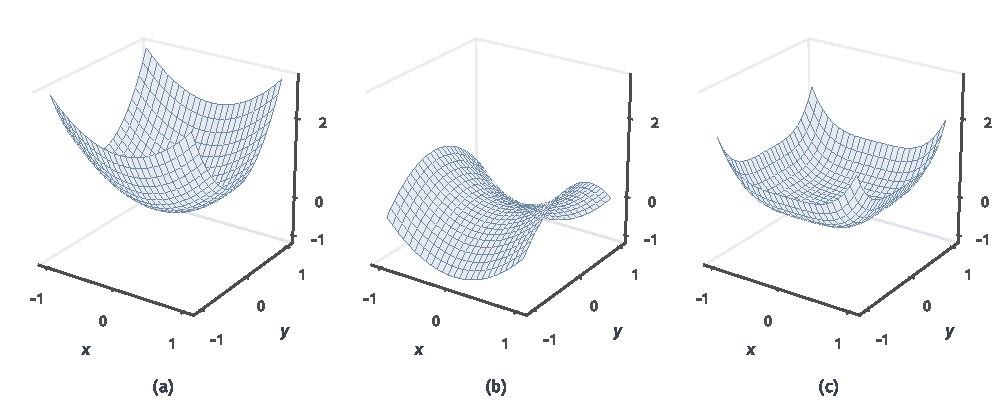
\includegraphics[width=169.0mm]{figures/00-shared/mathematical-preliminaries-upper/00-shared/matplotlib/chapter3-concept-processes/hessian-local-shapes.pdf}
 \caption{同一$[-1,1]^2$范围和纵轴尺度下，三面分别为$x^2+2y^2$、$x^2-y^2$、$x^4+y^4$。原点的Hessian依次为正定、不定、零矩阵；前两者给严格极小与鞍点，第三者虽严格极小却不能由正定判据推出。零Hessian也可能没有极值，例如前述$x^3$，故退化不是一种确定分类。}
 \label{fig:analysis-process-hessian-local-shapes}
\end{figure*}


\FloatBarrier
\section{本章小结}
\label{sec:multivariate-differentiation-chapter-summary}

本章的对象是位置上的量：标量场在每点给出一个数，向量场在每点给出一个与位置同维的向量，一般向量值函数的输出维数可以不同。它们的极限与连续性按输入、输出的范数理解，输出可以逐分量判断，输入的多个坐标却不能拆开逐个检查；沿两条路径得到不同极限能否定极限存在，只查若干条路径则不能证明它存在。

偏导数和方向导数只考察固定的直线。可微要求所有小扰动共用一个线性近似，包括方向随步长改变的扰动；这个近似由偏导数唯一确定。偏导数存在、全部方向导数存在或函数连续，都不单独保证可微；即使全部方向导数组成一个线性映射，仍须满足统一的余项条件。偏导数连续是方便的充分条件，但不是必要条件。

全微分是输入扰动上的线性泛函，梯度是它在所选内积下的表示向量。改变内积会改变梯度的坐标和最陡上升方向，全微分本身不变。沿含于定义域的线段，中值公式把梯度的大小化为有限变化的界；在凸开集上，梯度长度的统一上界恰好就是Lipschitz常数，凸性不能省略。

输出为向量时，微分由Jacobian矩阵表示，它的行是各分量的梯度，列是各输入坐标对输出点的推动。复合映射的Jacobian按计算顺序相乘，标量目标的梯度则由微分的伴随传回输入端。向量增量没有共同的中值点，改用沿线段的积分表示，并由导数的算子范数控制长度。

把微分再用于梯度，得到Hessian与二阶Taylor公式。混合偏导数在连续时可以交换，$C^2$函数的Hessian因而对称。在开集内的驻点处，Hessian正定、负定或不定分别对应严格极小、严格极大和鞍点；半定而退化的情形需要更高阶的信息，边界点和受约束的问题也不在这一判别的范围内。

这些结论都是局部的：可微只保证余项是$o(\lVert\bm h\rVert)$，不说明给定步长下误差有多大。矩阵自变量的微分公式、隐式方程确定的解，以及导数怎样控制误差放大和一阶预测的精度，依次在后面三章展开。


\chapter{矩阵函数的微分}
\label{sec:multivariable-matrix-perturbation}
\label{sec:multivariable-matrix-differentiation}
\label{chap:matrix-differentiation}

机器学习中的参数常排成矩阵，例如线性层的权重或协方差矩阵。损失是这些矩阵的标量函数，求逆、相乘等运算又产生矩阵输出。本章要回答：以矩阵为自变量时，微分是什么形状的对象；标量输出的梯度怎样读出；乘法、求逆、行列式与对数行列式这些常用运算的微分公式是什么，在哪里成立。

原则上可以把矩阵拉直成长向量，再用第~\ref{chap:multivariate-differentiation}章的结论。但保留矩阵形状，乘法次序与迹的结构更清楚，结果也能直接写成矩阵表达式。矩阵空间是有限维线性空间，所以本章不建立新的微分理论，而是把已有的全微分、链式法则与Riesz表示用于矩阵，集中处理三件事：矩阵的形状，乘法不交换，以及对称、正定等结构约束。

第一节说明矩阵变量的微分与Frobenius梯度，并区分全部扰动与结构受限的扰动。后四节依次处理基本运算、求逆、行列式和对数行列式。每种运算都先确定定义域与输入输出，再由增量的一阶项读出微分并验证可微性；能写出精确增量的运算，就用同一个代数展开完成这两件事。

本章只建立微分公式与梯度。这些公式给出的一阶预测在有限扰动下有多准、误差被放大多少，留到第~\ref{chap:differential-perturbation-analysis}章统一估计。本章用到第~\ref{chap:linear-operations}章的迹、Frobenius内积、行列式与逆矩阵，第~\ref{chap:dual-spaces}章的Riesz表示，以及第~\ref{chap:solution-error-regularization}章逆矩阵的有限扰动界。

\section{矩阵微分与梯度}
\label{sec:multivariable-matrix-variable-gradient}

$m\times n$矩阵输入可以看成$mn$个实数坐标，$r\times s$矩阵输出可以看成$rs$个实数分量。按固定顺序（例如逐列）把矩阵元素排成长向量，矩阵空间就等同于欧氏坐标空间；第~\ref{sec:prelim-matrix-trace}节的Frobenius内积与范数$\langle\bm A,\bm B\rangle_F=\operatorname{tr}(\bm A^\top\bm B)=\sum_{i,j}A_{i,j}B_{i,j}$，正是拉直后向量的欧氏内积与欧氏范数。
本章的定义域$\mathcal U$都是全矩阵空间$\mathbb R^{m\times n}$中的开集，基点$\bm X\in\mathcal U$，因此全部充分小的同形扰动都可以使用。

设$\Phi:\mathcal U\to\mathbb R^{r\times s}$。若存在矩阵空间之间的线性映射$\mathrm d\Phi_{\bm X}:\mathbb R^{m\times n}\to\mathbb R^{r\times s}$，使
\[
 \Phi(\bm X+\bm H)=\Phi(\bm X)+\mathrm d\Phi_{\bm X}(\bm H)+o(\lVert\bm H\rVert_F),
\]
余项按输出的Frobenius范数度量，则称$\Phi$在$\bm X$处可微，$\mathrm d\Phi_{\bm X}$为其微分。这就是向量值可微性按矩阵形状重排后的写法，计算时常写$\mathrm d\Phi=\mathrm d\Phi_{\bm X}(\mathrm d\bm X)$。$\mathrm d\Phi_{\bm X}$是从输入扰动空间到输出空间的线性映射，拉直后它的矩阵是$rs\times mn$的Jacobian，一般不能写成一个与$\bm X$同形的矩阵。

还要分清两类“矩阵的函数”。$\bm X\mapsto\bm X^{-1}$、$\bm X\mapsto\bm X^2$这类映射按矩阵运算定义，输出的每个元素一般依赖输入的许多元素；逐元素作用（例如对每个元素分别取指数）则把各元素分别送入一元函数，微分只在对应位置上相乘。第~\ref{sec:ls-matrix-functions}节由标量函数沿谱构造的矩阵函数$f(\bm S)$属于前一类，但只是以矩阵为输入的映射中的一种；它与逐元素作用不能混为一谈，研究$\bm S\mapsto f(\bm S)$的微分时，扰动一般也不保持原来的特征方向。

\paragraph{输入变量决定扰动的形状}
同一个表达式随所选变量不同，微分的输入也不同。固定$\bm A$时，$\bm x\mapsto\bm A\bm x$是线性映射，微分为$\bm h\mapsto\bm A\bm h$，扰动是向量；固定$\bm x$时，$\bm A\mapsto\bm A\bm x$也是线性映射，微分为$\bm E\mapsto\bm E\bm x$，扰动是矩阵。两者同时变化时，把$(\bm A,\bm x)$看作乘积空间$\mathbb R^{m\times n}\times\mathbb R^n$中的一个输入，取乘积范数$\lVert(\bm E,\bm h)\rVert=(\lVert\bm E\rVert_F^2+\lVert\bm h\rVert_2^2)^{1/2}$。精确增量
\[
 (\bm A+\bm E)(\bm x+\bm h)-\bm A\bm x=\bm A\bm h+\bm E\bm x+\bm E\bm h
\]
中，$\lVert\bm E\bm h\rVert_2\leq\lVert\bm E\rVert_F\lVert\bm h\rVert_2\leq\tfrac12\lVert(\bm E,\bm h)\rVert^2$，所以联合微分为$(\bm E,\bm h)\mapsto\bm A\bm h+\bm E\bm x$，余项$\bm E\bm h$对联合扰动是二次量。

\paragraph{标量输出与矩阵梯度}
输出为标量（$r=s=1$）时，$\mathrm df_{\bm X}$是矩阵空间上的线性泛函。矩阵空间取Frobenius内积，由Riesz表示定理（定理~\ref{thm:ls-riesz-representation}），这个泛函可以唯一写成与一个同形矩阵的内积，这个矩阵就是梯度。这与向量情形$\mathrm df_{\bm a}(\bm h)=\nabla f(\bm a)^\top\bm h$完全对应。
\begin{definition}[矩阵标量函数的梯度]
\label{def:multivariable-matrix-scalar-gradient}
设$f:\mathcal U\to\mathbb R$在$\bm X$处可微。唯一满足
\begin{equation}
 \mathrm df_{\bm X}(\bm H)=\langle\nabla_{\bm X}f,\bm H\rangle_F
 =\operatorname{tr}\bigl((\nabla_{\bm X}f)^\top\bm H\bigr)
\label{eq:analysis-matrix-gradient-definition}
\end{equation}
的同形矩阵$\nabla_{\bm X}f\in\mathbb R^{m\times n}$称为矩阵梯度。
\end{definition}
取只有第$(i,j)$个元素为$1$的扰动$\bm H$，右侧内积只剩$\nabla_{\bm X}f$的第$(i,j)$个元素，左侧是对$X_{i,j}$的偏导数。所以矩阵梯度的各元素就是对相应矩阵元素的偏导数，唯一性也由此得到。与向量梯度一样，在Frobenius长度下，$\nabla_{\bm X}f$指出使$f$增加最快的扰动方向。

求梯度的一般做法是：先展开微分，再利用迹的循环移位把扰动移到末端，写成$\operatorname{tr}(\bm G^\top\mathrm d\bm X)$的形式，便读出$\nabla_{\bm X}f=\bm G$。乘积形状相容时，
\[
 \begin{gathered}
\operatorname{tr}(\bm A\bm B)=\operatorname{tr}(\bm B\bm A)\\
\operatorname{tr}(\bm A\bm B\bm C)=\operatorname{tr}(\bm B\bm C\bm A).
 \end{gathered}
\]
这里循环移动的是整个因子，不能任意交换相邻矩阵。标量等于自己的迹，所以任何标量表达式都可以放进迹中再移位。
\begin{example}[双线性函数的矩阵梯度]
\label{ex:multivariable-bilinear-matrix-gradient}
对固定向量$\bm a\in\mathbb R^m$、$\bm b\in\mathbb R^n$，令$f(\bm W)=\bm a^\top\bm W\bm b$。它对$\bm W$线性，微分为$\mathrm df=\bm a^\top(\mathrm d\bm W)\bm b$。把这个标量写成迹并循环移位，
\[
 \mathrm df=\operatorname{tr}\bigl(\bm a^\top(\mathrm d\bm W)\bm b\bigr)=\operatorname{tr}\bigl(\bm b\bm a^\top\mathrm d\bm W\bigr)
 =\operatorname{tr}\bigl((\bm a\bm b^\top)^\top\mathrm d\bm W\bigr),
\]
于是$\nabla_{\bm W}f=\bm a\bm b^\top$。逐元素核对：$f=\sum_{k,l}a_kW_{k,l}b_l$，对$W_{i,j}$的偏导数是$a_ib_j$，正是$\bm a\bm b^\top$的第$(i,j)$个元素。
\end{example}

\paragraph{结构化变量的梯度}
矩阵梯度的唯一性用到了全部矩阵方向。若变量限制在线性子空间$\mathcal S$中，例如对称矩阵空间，允许的扰动只能取$\mathcal S$中的方向。在$\mathcal S$上沿用Frobenius内积，Riesz表示定理在$\mathcal S$内给出唯一的表示矩阵，称为受限梯度。设$f$在全矩阵空间中有可微的延拓，环境梯度为$\bm G$，记$P_{\mathcal S}$为到$\mathcal S$的正交投影。$\bm G-P_{\mathcal S}\bm G$与$\mathcal S$正交（第~\ref{sec:ls-orthogonal-projection}节），所以对$\bm H\in\mathcal S$有$\langle\bm G,\bm H\rangle_F=\langle P_{\mathcal S}\bm G,\bm H\rangle_F$：受限梯度就是环境梯度的正交投影。

对称矩阵空间中，任一矩阵分解为对称部分与反对称部分，二者Frobenius正交，因为对称$\bm S$与反对称$\bm K$满足$\operatorname{tr}(\bm S\bm K)=\operatorname{tr}((\bm S\bm K)^\top)=-\operatorname{tr}(\bm K\bm S)=-\operatorname{tr}(\bm S\bm K)$；因此投影为$(\bm G+\bm G^\top)/2$。若在$\mathcal S$中仍使用环境梯度，满足$\mathrm df(\bm H)=\langle\cdot,\bm H\rangle_F$（$\bm H\in\mathcal S$）的矩阵就不唯一：$\bm G$加上任一与$\mathcal S$正交的矩阵都满足。

对称正定矩阵组成对称矩阵空间中的开集：由第~\ref{chap:condition-and-spectral-perturbation}章的Weyl界，对称扰动的谱范数小于最小特征值时正定性保持。所以讨论正定变量时，邻域和扰动方向都在对称子空间内理解。矩阵输出时没有这样的单个梯度矩阵，只能保留线性映射$\mathrm d\Phi_{\bm X}$本身。

\section{基本矩阵运算的微分}
\label{sec:multivariable-matrix-basic-operations}

本节从最简单的矩阵运算开始。线性运算的余项为零；乘法与平方的增量可以直接展开，微分之外剩下的部分就是可以精确写出的余项，由它验证可微性；迹、Frobenius范数平方与二次型则用来练习读出梯度。

\paragraph{线性运算}
加法、固定标量的数乘、转置与迹都是线性映射，精确增量就是它们作用于扰动的结果，余项为零，所以微分等于运算本身：
\[
 \begin{gathered}
 \mathrm d(\bm X+\bm Y)=\mathrm d\bm X+\mathrm d\bm Y,\\
 \mathrm d(c\bm X)=c\,\mathrm d\bm X,\\
 \mathrm d(\bm X^\top)=(\mathrm d\bm X)^\top,\\
 \mathrm d\operatorname{tr}\bm X=\operatorname{tr}(\mathrm d\bm X).
 \end{gathered}
\]
固定矩阵从两侧相乘也是线性的：$\mathrm d(\bm A\bm X\bm B)=\bm A(\mathrm d\bm X)\bm B$，扰动夹在中间的位置不能移动。复合运算沿用第~\ref{sec:analysis-vector-chain-matrix-calculus}节的链式法则：先计算内部扰动，再让外部微分作用于它。只要逐步核对每个线性映射的输入、输出形状，就不需要另背一套矩阵求导规则。

线性迹函数的微分已经是式~\eqref{eq:analysis-matrix-gradient-definition}的形式，可以直接读出梯度。对固定的$\bm{A}\in\mathbb{R}^{m\times n}$，令$f(\bm{X})=\operatorname{tr}(\bm{A}^{\top}\bm{X})=\sum_{i,j}A_{i,j}X_{i,j}$。由于$f$线性，$f(\bm X+\bm H)-f(\bm X)=\operatorname{tr}(\bm A^\top\bm H)$，没有余项，所以
\begin{equation}
  \nabla_{\bm{X}}\operatorname{tr}(\bm{A}^{\top}\bm{X})
  =\bm{A}.
\label{eq:analysis-trace-linear-gradient}
\end{equation}
这与向量情形$\nabla_{\bm x}(\bm a^\top\bm x)=\bm a$对应，常用于从迹表达式中读出梯度。

\paragraph{乘积的精确增量}
两个因子同时变化时，只用分配律就得到
\begin{equation}
 (\bm A+\bm E)(\bm B+\bm H)-\bm A\bm B=\bm A\bm H+\bm E\bm B+\bm E\bm H .
\label{eq:multivariable-product-increment}
\end{equation}
这一等式对任意大小的扰动都成立，本身不涉及微分。前两项对$(\bm E,\bm H)$线性，各被另一个因子放大：在满足乘积不等式的矩阵范数下，$\lVert\bm A\bm H+\bm E\bm B\rVert\leq\lVert\bm A\rVert\lVert\bm H\rVert+\lVert\bm E\rVert\lVert\bm B\rVert$。要把它们识别为微分，还须选定联合输入的大小，例如$\lVert(\bm E,\bm H)\rVert=(\lVert\bm E\rVert_F^2+\lVert\bm H\rVert_F^2)^{1/2}$。由Frobenius范数的次乘性，
\[
 \lVert\bm E\bm H\rVert_F\leq\lVert\bm E\rVert_F\lVert\bm H\rVert_F\leq\tfrac12\lVert(\bm E,\bm H)\rVert^2 ,
\]
交叉项除以联合扰动的大小后趋于零。所以
\[
 \mathrm D(\bm A\bm B)[\bm E,\bm H]=\bm A\bm H+\bm E\bm B,
\]
而$\bm E\bm H$是可以直接计算的精确余项。只固定一个因子时，乘积对另一个因子线性，交叉项不出现。

令两因子相同，$\Phi(\bm X)=\bm X^2$的精确增量为$(\bm X+\bm E)^2-\bm X^2=\bm X\bm E+\bm E\bm X+\bm E^2$。由$\lVert\bm E^2\rVert_F\leq\lVert\bm E\rVert_F^2$，得到$\mathrm d(\bm X^2)(\bm E)=\bm X\bm E+\bm E\bm X$，余项恰为$\bm E^2$。只有$\bm X$与扰动交换时，才能写成$2\bm X\bm E$。例如
\[
 \bm X=\begin{bmatrix}0&1\\0&0\end{bmatrix},\qquad
 \bm E=\begin{bmatrix}0&0\\1&0\end{bmatrix}
\]
时，$\bm X\bm E=\operatorname{diag}(1,0)$、$\bm E\bm X=\operatorname{diag}(0,1)$，正确的一阶项是$\bm I$，而照搬标量规则的$2\bm X\bm E=\operatorname{diag}(2,0)$是错的。直接核对：$(\bm X+t\bm E)^2=t\bm I$，对$t$的导数正是$\bm I$；本例中$\bm E^2=\bm 0$，余项为零。

\paragraph{Frobenius范数平方与二次型}
标量值运算的微分可以直接读出梯度。双线性形式$\bm a^\top\bm W\bm b$已在示例~\ref{ex:multivariable-bilinear-matrix-gradient}中处理。Frobenius范数平方的精确增量为
\[
 \lVert\bm X+\bm E\rVert_F^2-\lVert\bm X\rVert_F^2=2\langle\bm X,\bm E\rangle_F+\lVert\bm E\rVert_F^2 ,
\]
所以$\nabla_{\bm X}\lVert\bm X\rVert_F^2=2\bm X$，余项恰为$\lVert\bm E\rVert_F^2$。

同一个数组在固定线性作用和可变输入两种角色下，会产生不同的导数，二次型$\bm x^\top\bm A\bm x$是典型的例子。固定$\bm A$、以$\bm x$为变量时，由式~\eqref{eq:analysis-quadratic-form-gradient}，梯度为$(\bm A+\bm A^\top)\bm x$，是向量；固定$\bm x$、以$\bm A$为变量时，$\bm x^\top\bm E\bm x=\operatorname{tr}(\bm x\bm x^\top\bm E)=\langle\bm x\bm x^\top,\bm E\rangle_F$，梯度为$\bm x\bm x^\top$，是矩阵，且没有余项。两者同时变化时，展开得
\[
 \begin{aligned}
 &(\bm x+\bm h)^\top(\bm A+\bm E)(\bm x+\bm h)-\bm x^\top\bm A\bm x\\
 &\quad=\bm x^\top(\bm A+\bm A^\top)\bm h+\bm x^\top\bm E\bm x
 +\bigl(\bm h^\top\bm A\bm h+\bm x^\top\bm E\bm h+\bm h^\top\bm E\bm x+\bm h^\top\bm E\bm h\bigr).
 \end{aligned}
\]
括号中的每一项都至少含两个扰动因子，对联合扰动是高阶量，所以联合微分是两个单独微分之和：$(\bm E,\bm h)\mapsto\bm x^\top(\bm A+\bm A^\top)\bm h+\bm x^\top\bm E\bm x$。

\section{求逆的微分}
\label{sec:multivariable-inverse-differential}

求逆映射$\operatorname{inv}(\bm A)=\bm A^{-1}$定义在$d\times d$可逆矩阵组成的集合上，输入、输出都是方阵，属于矩阵输出的情形，没有单个梯度矩阵，要直接求微分。逆矩阵与行列式非零的关系已在第~\ref{sec:prelim-inverse-matrices}节及第~\ref{sec:prelim-determinants}节建立。本节的矩阵范数取由向量范数诱导的矩阵范数，它使$\lVert\bm I\rVert=1$并满足乘积不等式。

\paragraph{由逆差恒等式得到微分}
设$\bm A$可逆，$\bm B=\bm A+\bm E$，并设$q=\lVert\bm A^{-1}\rVert\lVert\bm E\rVert<1$。第~\ref{sec:ls-inverse-sensitivity}节已经证明，这时$\bm B$可逆，逆差满足精确恒等式~\eqref{eq:ch06-inverse-finite-perturbation}，即$\bm B^{-1}-\bm A^{-1}=-\bm B^{-1}\bm E\bm A^{-1}$，并且
\[
 \lVert\bm B^{-1}-\bm A^{-1}\rVert\leq\frac{\lVert\bm A^{-1}\rVert^2\lVert\bm E\rVert}{1-q}.
\]
特别地，可逆矩阵组成开集，而且$\bm E\to\bm0$时$\bm B^{-1}\to\bm A^{-1}$，求逆是连续的。

恒等式右端含未知的$\bm B^{-1}$，还不是对$\bm E$线性的式子。把其中的$\bm B^{-1}$换成$\bm A^{-1}$，就得到线性的候选项$-\bm A^{-1}\bm E\bm A^{-1}$。替换造成的差为
\[
 \bm B^{-1}-\bm A^{-1}+\bm A^{-1}\bm E\bm A^{-1}
 =-(\bm B^{-1}-\bm A^{-1})\bm E\bm A^{-1},
\]
其范数不超过$\lVert\bm B^{-1}-\bm A^{-1}\rVert\,\lVert\bm E\rVert\,\lVert\bm A^{-1}\rVert$。由上面的连续性，第一个因子随$\bm E\to\bm0$趋于零，所以这个差是$o(\lVert\bm E\rVert)$。有限维矩阵空间中各种范数等价，对Frobenius范数同样如此。因此求逆在每个可逆矩阵处可微，且
\begin{equation}
  \mathrm{d}(\bm{X}^{-1})
  =
  -\bm{X}^{-1}(\mathrm{d}\bm{X})\bm{X}^{-1}.
\label{eq:analysis-inverse-differential}
\end{equation}
这个导数以矩阵方向$\mathrm d\bm X$为输入，输出仍是同形的方阵；它是矩阵空间上的线性映射，不能写成单个梯度矩阵。上面的差还可以精确写出并给出二次界，这在第~\ref{sec:multivariable-inverse-perturbation}节用于估计一阶预测的误差。

这里先由精确恒等式确认了可微性。随后可以对恒等式$\bm{X}\bm{X}^{-1}=\bm{I}$两侧求微分作交叉核对：左侧用乘积法则，右侧是常矩阵，得到$(\mathrm{d}\bm{X})\bm{X}^{-1}+\bm{X}\,\mathrm{d}(\bm{X}^{-1})=\bm{0}$，左乘$\bm{X}^{-1}$便回到同一公式。这一形式推导以逆映射可微为前提，不能单独承担可微性的证明。

$1\times1$时这就是$(1/x)'=-1/x^2$。两个$\bm{X}^{-1}$位于扰动两侧，不能合并成$-\bm{X}^{-2}\mathrm{d}\bm{X}$，因为$\mathrm{d}\bm{X}$未必与$\bm{X}^{-1}$交换。
取一个对角矩阵和一个非对角扰动，就能看出两种写法的差别。
\begin{example}[逆矩阵微分中的乘法次序]
\label{ex:analysis-noncommuting-inverse-differential}
取$\bm X=\operatorname{diag}(2,1)$，扰动方向
\[
 \bm E=\begin{bmatrix}0&1\\1&0\end{bmatrix}.
\]
由式~\eqref{eq:analysis-inverse-differential}，沿$\bm X+t\bm E$求逆矩阵在$t=0$处的导数为
\[
 -\bm X^{-1}\bm E\bm X^{-1}
 =\begin{bmatrix}0&-1/2\\-1/2&0\end{bmatrix}.
\]
若照搬标量规则而写成$-\bm X^{-2}\bm E$，会得到
\[
 \begin{bmatrix}0&-1/4\\-1&0\end{bmatrix}.
\]
两种写法给出不同的矩阵。要判断哪一个正确，可以直接写出这条路径上的逆矩阵：
\[
 (\bm X+t\bm E)^{-1}=\frac1{2-t^2}\begin{bmatrix}1&-t\\-t&2\end{bmatrix}.
\]
在$t=0$处对$t$求导，两个非对角元的导数都是$-1/2$，对角元的导数为$0$，与第一种结果一致。
\end{example}

错误写法连对称性都丢失了。路径$\bm X+t\bm E$在$t=0$附近由对称可逆矩阵组成，它们的逆也对称，所以导数必须对称。这种结构检查能直接发现错误。

矩阵沿可微的参数曲线$\bm A(t)$变化，且每个$\bm A(t)$可逆时，链式法则与式~\eqref{eq:analysis-inverse-differential}给出
\[
 \frac{\mathrm d}{\mathrm dt}\bm A(t)^{-1}=-\bm A(t)^{-1}\bm A'(t)\bm A(t)^{-1}.
\]
第~\ref{sec:multivariable-logdet-differential}节和第~\ref{chap:differential-perturbation-analysis}章沿扰动线段求导时都会用到这个公式。

\section{行列式的微分}
\label{sec:multivariable-determinant-differential}

行列式把方阵映为一个实数，它的绝对值是线性映射对体积的缩放倍数（第~\ref{sec:prelim-determinants}节）。按排列展开，$\det\bm A$是各元素的多项式，所以它在全部方阵上连续可微，奇异矩阵处也不例外。本节由逐列展开算出微分，再在可逆时化为迹的形式。
\paragraph{代数余子式形式}
行列式对每一列分别线性（第~\ref{sec:prelim-determinants}节）。记$\bm A\in\mathbb R^{d\times d}$的列为$\bm a_1,\ldots,\bm a_d$，扰动$\bm E$的列为$\bm e_1,\ldots,\bm e_d$，逐列展开$\det(\bm a_1+\bm e_1,\ldots,\bm a_d+\bm e_d)$，得到$2^d$项，每一项在每一列取$\bm a_j$或$\bm e_j$。全取$\bm a_j$的一项是$\det\bm A$；恰有第$j$列取$\bm e_j$的一项，按第$j$列展开（第~\ref{sec:ls-det-cofactor-adjugate}节）等于$\sum_iE_{i,j}C_{i,j}$，其中$C_{i,j}$是$\bm A$的代数余子式，它不依赖$\bm A$的第$j$列。其余各项至少含两列扰动，是$\bm E$的元素的多项式，且每个单项至少二次；由$|E_{i,j}|\leq\lVert\bm E\rVert_F$，在$\lVert\bm E\rVert_F\leq1$时它们的和不超过某个常数乘$\lVert\bm E\rVert_F^2$。于是
\begin{equation}
 \mathrm d\det_{\bm A}(\bm E)=\sum_{i,j}C_{i,j}E_{i,j}=\langle\bm C,\bm E\rangle_F=\operatorname{tr}\bigl(\operatorname{adj}(\bm A)\bm E\bigr),
\label{eq:multivariable-determinant-cofactor-differential}
\end{equation}
其中$\bm C=[C_{i,j}]$是代数余子式矩阵，$\operatorname{adj}(\bm A)=\bm C^\top$是古典伴随。Frobenius梯度为$\nabla_{\bm A}\det=\bm C$。这个公式在奇异矩阵处同样成立。

$\bm A$可逆时，古典伴随恒等式（定理~\ref{thm:ls-adjugate-identity}）给出$\operatorname{adj}(\bm A)=\det(\bm A)\bm A^{-1}$，代入得到Jacobi公式的一阶形式
\[
 \mathrm{d}\det\bm{X}=\det(\bm{X})\operatorname{tr}(\bm{X}^{-1}\mathrm{d}\bm{X}),
\]
相应的梯度为$\det(\bm X)\bm X^{-\top}$。它说明有向体积缩放倍数的相对变化为
\[
 \frac{\mathrm d\det\bm X}{\det\bm X}=\operatorname{tr}(\bm X^{-1}\mathrm d\bm X).
\]
也可以用乘法公式核对：
\[
 \det(\bm X+\bm H)=\det(\bm X)\det(\bm I+\bm X^{-1}\bm H),
\]
问题化归为单位矩阵附近的一阶变化。奇异处没有$\bm X^{-1}$，只能使用代数余子式或古典伴随的形式。

在最简单的基点$\bm I$处，代数余子式矩阵就是$\bm I$，一阶变化是扰动的迹。
\begin{example}[单位矩阵附近行列式的一阶变化]
\label{ex:multivariable-determinant-near-identity}
取$\bm H=\operatorname{diag}(\varepsilon_1,\varepsilon_2)$，则
\[
 \det(\bm I+\bm H)=(1+\varepsilon_1)(1+\varepsilon_2)=1+\varepsilon_1+\varepsilon_2+\varepsilon_1\varepsilon_2,
\]
一阶变化是$\varepsilon_1+\varepsilon_2=\operatorname{tr}\bm H$。若扰动只在非对角位置，例如
\[
 \bm H=\begin{bmatrix}0&\varepsilon\\0&0\end{bmatrix},
\]
则$\det(\bm I+\bm H)=1$，面积不变，而$\operatorname{tr}\bm H=0$。
\end{example}

两个方向各拉长一点时，面积的相对增量一阶上是两个伸长率之和；剪切扰动不改变面积，迹也为零。两种情形中，一阶变化都等于扰动的迹。

\section{对数行列式的微分}
\label{sec:multivariable-logdet-differential}

实值的$\log\det\bm A$要求$\det\bm A>0$。行列式连续，满足这一条件的方阵组成开集，对数在其上与行列式复合。对行列式的微分应用标量对数的链式法则$\mathrm d\log u=\mathrm du/u$，得到
\begin{equation}
\begin{gathered}
\mathrm{d}\log\det\bm{X}
  =
  \operatorname{tr}(\bm{X}^{-1}\mathrm{d}\bm{X})\\
\nabla_{\bm{X}}\log\det\bm{X}
  =
  \bm{X}^{-\top}.
\end{gathered}
\label{eq:analysis-logdet-gradient}
\end{equation}
第二式由$\operatorname{tr}(\bm X^{-1}\mathrm d\bm X)=\operatorname{tr}\bigl((\bm X^{-\top})^\top\mathrm d\bm X\bigr)$对照式~\eqref{eq:analysis-matrix-gradient-definition}读出。
若$\bm X$还对称，则$\bm{X}^{-\top}=\bm{X}^{-1}$；一般情形应保留转置。$1\times1$时它回到$(\log x)'=1/x$。

\paragraph{对称正定变量}
统计与优化中常见的是对称正定矩阵上的$\log\det$。这时变量在对称矩阵子空间中，只允许对称扰动。由第~\ref{sec:multivariable-matrix-variable-gradient}节，受限梯度是环境梯度$\bm A^{-\top}=\bm A^{-1}$在对称子空间上的投影；它本身已对称，所以梯度就是$\bm A^{-1}$。

这里有两个不同的定义域。$\det>0$的方阵组成全矩阵空间中的开集，$\log\det$在其上已有定义，式~\eqref{eq:analysis-logdet-gradient}在这个开集上处处成立；对称正定矩阵组成对称子空间中的开集，是前者与对称子空间之交的一部分。所以正定性不是$\log\det$可微的条件，它只决定允许的扰动方向和梯度的表示。第~\ref{sec:multivariable-logdet-perturbation}节估计有限扰动下的余项时，正定性还提供整条扰动线段留在定义域内的明确保证。

\FloatBarrier
\section{本章小结}
\label{sec:matrix-differentiation-summary}

以矩阵为自变量时，微分仍是全部同形扰动上的线性映射，只是保留了矩阵形状。标量输出时，Riesz表示在Frobenius内积下给出同形的梯度矩阵，常用的读法是把微分写成$\operatorname{tr}(\bm G^\top\mathrm d\bm X)$；矩阵输出时没有单个梯度矩阵，只能保留微分本身，例如求逆的$\mathrm d\bm X\mapsto-\bm X^{-1}\mathrm d\bm X\bm X^{-1}$。变量限制在对称矩阵等子空间时，允许的方向随之受限，受限梯度是环境梯度的正交投影，对称情形为$(\bm G+\bm G^\top)/2$。

各运算的公式与条件可以这样归纳。线性运算的微分就是运算本身；乘积的微分是两个“只变一个因子”的项之和，因子顺序不能交换，平方的微分是$\bm X\mathrm d\bm X+\mathrm d\bm X\bm X$而不是$2\bm X\mathrm d\bm X$。求逆在可逆矩阵的开集上可微，扰动夹在两个逆矩阵之间。行列式是多项式，在包括奇异矩阵的全部方阵上可微，微分由代数余子式给出，可逆时化为$\det(\bm X)\operatorname{tr}(\bm X^{-1}\mathrm d\bm X)$。对数行列式在$\det>0$的开集上可微，梯度为$\bm X^{-\top}$，对称正定情形化为$\bm X^{-1}$。

所有公式都先由增量的一阶项识别、再由余项验证可微，对$\bm X\bm X^{-1}=\bm I$等恒等式形式求导只能作核对。精确增量中的余项本章只用来证明可微；这些公式作为一阶工具，在第~\ref{chap:differential-perturbation-analysis}章用来估计条件数和有限扰动下一阶预测的误差。

\chapter{隐函数与反函数}
\label{sec:analysis-implicit-parameter-integral}
\label{chap:implicit-inverse-functions}

前面各章对给定的显式映射求微分。本章反过来从方程出发：给定一组方程，判断它能否在基点附近确定唯一的函数，并求这个函数的导数。

实际问题中，变量之间常由约束联系，而不是由显式公式给出。单位圆上的点满足$x^2+y^2=1$，物理系统的平衡状态满足力的平衡方程，训练得到的最优参数满足梯度为零。我们关心的是：一部分变量（参数）稍作改变时，其余变量（未知量）是否随之唯一地、光滑地改变，变化率又是多少。

方程组用向量值映射表示。方程个数与待解变量个数相同时，关于待解变量的方阵Jacobian是否可逆，决定了能否在局部解出这些变量。第一节建立隐函数定理：先用例子说明为什么必须指定起始解、为什么条件落在待解变量的导数上，再用压缩迭代证明局部解的存在、唯一与可微，最后给出导数公式。第二节把输出当作参数、输入当作待解变量，由隐函数定理得到局部反函数定理，并说明局部可逆不能推出整体单射。

证明要用到第~\ref{chap:multivariate-differentiation}章的链式法则、向量值中值估计与压缩的概念，以及第~\ref{chap:normed-inner-product-spaces}章有限维空间的完备性。本章只回答解是否存在、是否唯一、怎样求导。隐式给定的特征值与特征向量分支对矩阵扰动的响应有多大，在第~\ref{chap:differential-perturbation-analysis}章用这里的定理分析。

\section{隐函数的存在与微分}
\label{sec:multivariable-implicit-function}

显式函数直接给出输出，例如$y=\sqrt x$。关系$F(x,y)=0$则没有直接说明给定$x$时$y$取什么值：满足方程的$y$可能有多个，也可能一个都没有。

设$(a,b)$满足$F(a,b)=0$。若存在$a$附近的区间$I$、$b$附近的区间$J$和函数$\varphi:I\to J$，使得对$I\times J$中的点，$F(x,y)=0$成立恰好当$y=\varphi(x)$，就称方程在$(a,b)$附近确定了一个\term{隐函数}（implicit function）$y=\varphi(x)$。换句话说，只看$(a,b)$附近的小矩形，方程的解集恰是一个函数的图像。
因此先要说明局部解分支存在且唯一，然后才能对这条分支求导。

同一个方程在一些点附近确定隐函数，在另一些点附近则不确定。
\begin{example}[单位圆附近的隐函数]
\label{ex:multivariable-implicit-circle}
考虑单位圆$x^2+y^2-1=0$。在$(0,1)$附近，解集是上半圆$y=\sqrt{1-x^2}$的一段；在$(0,-1)$附近则是下半圆$y=-\sqrt{1-x^2}$的一段，两处都确定了隐函数。
但在$(1,0)$附近，每个略小于$1$的$x$对应上下两个解，略大于$1$的$x$没有解；无论矩形多小，解集都不是关于$x$的函数图像。此处圆的切线是竖直的。
\end{example}

解集分成几支时，还要指定从哪一个解出发。
\begin{example}[方程$y^2=x$的两支解]
\label{ex:multivariable-implicit-parabola-branches}
方程$y^2-x=0$在$x>0$时有正、负两支解$y=\pm\sqrt x$。固定其中一个非零解，例如$(1,1)$，可以在它附近选出唯一的正支。
但在$(0,0)$处两支相交，负$x$侧又没有实数解，因此不存在定义在含$0$的开区间上的解函数。
\end{example}

两个例子中不能局部解出$y$的点，都满足$\partial F/\partial y=2y=0$：单位圆在$(1,0)$处如此，$y^2-x$在$(0,0)$处也如此。下面的定理~\ref{thm:analysis-implicit-function}要求的可逆性，恰好在这些点失效。所以局部选解既要指定起始解，也要核对关于待解变量的导数。

换一个被解变量，非退化条件也随之改变：单位圆在$(1,0)$处虽不能把$y$解成$x$的函数，却有$\partial F/\partial x=2\neq0$，可以在附近把$x$解成$y$的函数$x=\sqrt{1-y^2}$。

图~\ref{fig:vol1-add-implicit-branches}显示“局部唯一”怎样排除另一支解。在$(1,1)$附近只保留正支即可；在原点处，两支相交且负$x$没有实数解，不能这样局部选出可微的解。
\begin{figure}[!htb]
  \centering
  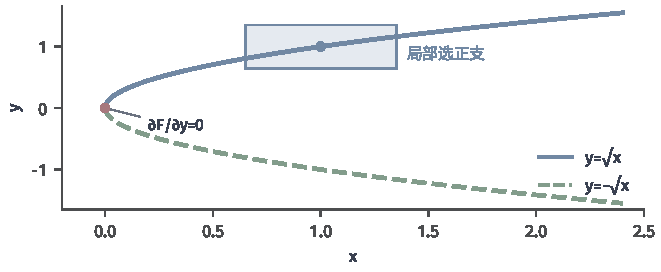
\includegraphics[width=112mm]{figures/00-shared/mathematical-preliminaries-upper/00-shared/matplotlib/mathematical-language-combinatorics-analysis-optimization-comprehension-additions/implicit-branches.pdf}
  \caption{方程$F(x,y)=y^2-x=0$的两支实数解。浅蓝矩形围住$(1,1)$，在该矩形内每个允许的$x$只有正支解，且$F_y=2y\neq0$；红点处$F_y=0$，两支相交。两支解满足同一方程，选定起始解与邻域才确定隐函数分支。}
  \label{fig:vol1-add-implicit-branches}
\end{figure}
\FloatBarrier


\paragraph{存在、唯一性与微分}

条件之所以落在关于待解变量的导数上，可以从线性方程看出来。

设$\bm x\in\mathbb R^p$为参数、$\bm y\in\mathbb R^m$为未知量，$\bm P\in\mathbb R^{m\times p}$、$\bm Q\in\mathbb R^{m\times m}$固定，方程$\bm P\bm x+\bm Q\bm y=\bm 0$有$m$个方程、$m$个未知量。当$\bm Q$可逆时，对每个$\bm x$都有唯一解
\[
 \bm y=-\bm Q^{-1}\bm P\bm x;
\]
$\bm Q$不可逆时，对给定的$\bm x$，解要么不存在，要么不唯一。

对非线性方程$F(\bm x,\bm y)=\bm 0$，可微性说明它在基点附近近似于线性方程
\[
 \bm D_{\bm x}F(\bm a,\bm b)(\bm x-\bm a)+\bm D_{\bm y}F(\bm a,\bm b)(\bm y-\bm b)\approx\bm 0,
\]
其中$\bm D_{\bm x}F$、$\bm D_{\bm y}F$分别是只对$\bm x$、只对$\bm y$的坐标求偏导排成的Jacobian块。隐函数定理断言：只要线性近似中$\bm Q=\bm D_{\bm y}F$可逆，非线性方程在局部也像线性方程一样有唯一解，而且解的导数就是线性解的系数$-\bm Q^{-1}\bm P$。

定理给出的是充分条件。它只要求待解变量对应的方阵Jacobian可逆，不要求整个带参数映射的Jacobian是方阵。
\begin{theorem}[隐函数定理]
\label{thm:analysis-implicit-function}
设$F:\mathbb{R}^p\times\mathbb{R}^m\to\mathbb{R}^m$在$(\bm{a},\bm{b})$的某个开邻域内连续可微，$F(\bm{a},\bm{b})=\bm{0}$，并且关于待解变量的Jacobian矩阵
\[
 \bm{D}_{\bm{y}}F(\bm{a},\bm{b})\in\mathbb{R}^{m\times m}
\]
可逆。则存在$\bm{a}$与$\bm{b}$的邻域$U,V$，以及唯一的连续可微函数
$\varphi:U\to V$，使$\varphi(\bm{a})=\bm{b}$，并且对所有
$(\bm{x},\bm{y})\in U\times V$都有
\[
  F(\bm{x},\bm{y})=\bm{0}
  \quad\Longleftrightarrow\quad
  \bm{y}=\varphi(\bm{x}).
\]
其Jacobian矩阵满足
\begin{equation}
  \begin{aligned}
  \bm{D}\varphi(\bm{x})
  ={}&-\bigl[\bm{D}_{\bm{y}}F(\bm{x},\varphi(\bm{x}))\bigr]^{-1}\\
  &\cdot\bm{D}_{\bm{x}}F(\bm{x},\varphi(\bm{x})).
  \end{aligned}
\label{eq:analysis-implicit-derivative}
\end{equation}
\end{theorem}
矩阵形状为$(m\times m)(m\times p)=m\times p$，与$\varphi:\mathbb R^p\to\mathbb R^m$的Jacobian一致。唯一性只限于所选的邻域$U\times V$：定理不排除远处还有满足同一方程的其他解支，例如$y^2=x$在$(1,1)$附近选出正支，负支仍然存在。

若已知$\varphi$存在且可微，导数公式可以直接由链式法则得到：对恒等式$F(\bm x,\varphi(\bm x))=\bm 0$求导，得
\[
 \bm D_{\bm x}F+\bm D_{\bm y}F\,\bm D\varphi=\bm 0,
\]
再左乘$(\bm D_{\bm y}F)^{-1}$。定理真正困难的部分是$\varphi$的存在、唯一与可微，形式求导不能替代这些步骤。

证明的思路是把解方程改写为反复修正的迭代。一元时，固定$x$，从$y_0=b$出发，用
\[
 y_{n+1}=y_n-\frac{F(x,y_n)}{F_y(a,b)}
\]
不断修正：若$F(x,y_n)>0$且$F_y(a,b)>0$，就把$y$调小一点。这类似Newton法，只是斜率固定用基点处的值。若每次修正都使误差按固定比例缩小，迭代就收敛到唯一解。

证明依次检查三件事：修正映射是压缩；它不把点送出所考察的球；所得解随参数可微。
\begin{proof}
先把方程改写为局部压缩迭代。记
\[
 \begin{gathered}
\bm{A}=\bm{D}_{\bm{y}}F(\bm{a},\bm{b})\\
T_{\bm{x}}(\bm{y})=\bm{y}-\bm{A}^{-1}F(\bm{x},\bm{y}).
 \end{gathered}
\]
因为$\bm A^{-1}$可逆，$F(\bm{x},\bm{y})=\bm{0}$当且仅当$T_{\bm{x}}(\bm{y})=\bm{y}$，即$\bm y$是更新后保持不变的点，称为不动点。并且
\[
 \bm{D}_{\bm{y}}T_{\bm{x}}(\bm{y})=\bm{I}-\bm{A}^{-1}\bm{D}_{\bm{y}}F(\bm{x},\bm{y}),
\]
它在$(\bm{a},\bm{b})$处为零。

由$F$的导数连续，这个矩阵的元素在基点附近都很小；又谱范数不超过Frobenius范数（第~\ref{sec:multivariable-operator-norm}节）。因而可以选择闭球$B=\{\bm{y}:\lVert\bm{y}-\bm{b}\rVert_2\leq r\}$和$\bm{a}$的邻域$U$，使
\begin{equation}
  \sup_{\bm{x}\in U,\,\bm{y}\in B}
  \left\lVert
    \bm{D}_{\bm{y}}T_{\bm{x}}(\bm{y})
  \right\rVert_2
  \leq q<1.
\label{eq:analysis-ift-uniform-contraction}
\end{equation}
沿$\bm{y}$方向使用式~\eqref{eq:analysis-operator-mean-value-bound}（球是凸集，球内线段不离开球）可知，每个
$T_{\bm{x}}$都把$B$内任意两点之间的距离缩小到原来的至多$q$倍。

还必须核对自映射，即$T_{\bm x}$不把$B$中的点送出$B$；否则迭代可能离开压缩成立的范围。因为$T_{\bm{a}}(\bm{b})=\bm{b}$且$T_{\bm{x}}(\bm{b})$关于$\bm{x}$连续，可进一步缩小$U$，使
\[
 \lVert T_{\bm{x}}(\bm{b})-\bm{b}\rVert_2\leq\frac{1-q}{2}r.
\]
于是对$\bm{y}\in B$，先用三角不等式拆开，再用压缩性，
\[
 \begin{aligned}
  \lVert T_{\bm{x}}(\bm{y})-\bm{b}\rVert_2
  &\leq
  \lVert T_{\bm{x}}(\bm{y})-T_{\bm{x}}(\bm{b})\rVert_2+\lVert T_{\bm{x}}(\bm{b})-\bm{b}\rVert_2\\
  &\leq
  q\lVert\bm{y}-\bm{b}\rVert_2+\frac{1-q}{2}r
  \leq
  \frac{1+q}{2}r
  <r.
 \end{aligned}
\]
所以$T_{\bm{x}}(B)$包含在$B$的内部$V$中。

固定$\bm x\in U$，从$\bm y_0=\bm b$出发，令$\bm y_{n+1}=T_{\bm x}(\bm y_n)$。
所有迭代项都留在$B$内，每一步的压缩使相邻差满足
\[
 \begin{aligned}
 \lVert\bm y_{n+1}-\bm y_n\rVert_2
 &\leq q\lVert\bm y_n-\bm y_{n-1}\rVert_2\\
 &\leq\cdots\leq q^n\lVert\bm y_1-\bm y_0\rVert_2.
 \end{aligned}
\]
增大$q$仍保留这个上界，因而可设$0<q<1$。对$m'>n$，几何和给出
\[
 \lVert\bm y_{m'}-\bm y_n\rVert_2
 \leq\sum_{j=n}^{m'-1}\lVert\bm y_{j+1}-\bm y_j\rVert_2
 \leq\frac{q^n}{1-q}\lVert\bm y_1-\bm y_0\rVert_2\longrightarrow0,
\]
所以$(\bm y_n)$是Cauchy列。有限维赋范空间完备（定理~\ref{thm:ls-finite-dimensional-complete}），该序列收敛；闭性使极限仍在$B$内。

$T_{\bm x}$连续，在$\bm y_{n+1}=T_{\bm x}(\bm y_n)$中令$n\to\infty$，可得极限$\varphi(\bm x)$满足
\[
 T_{\bm x}(\varphi(\bm x))=\varphi(\bm x),
\]
而$T_{\bm x}(B)\subset V$使它属于$V$。

若另有不动点$\bm z\in B$，则
\[
 \begin{aligned}
 \lVert\bm z-\varphi(\bm x)\rVert_2
 &=\lVert T_{\bm x}(\bm z)-T_{\bm x}(\varphi(\bm x))\rVert_2\\
 &\leq q\lVert\bm z-\varphi(\bm x)\rVert_2,
 \end{aligned}
\]
由$q<1$只能有$\bm z=\varphi(\bm x)$，所以这个不动点唯一。若
$(\bm{x},\bm{y})\in U\times V$且$F(\bm{x},\bm{y})=\bm{0}$，则$\bm{y}\in B$也是
$T_{\bm{x}}$的不动点，唯一性迫使$\bm{y}=\varphi(\bm{x})$。这证明了定理所述的局部
存在与零点集合的逐点唯一性。

还需说明所得解随参数连续可微。先证$\varphi$局部Lipschitz连续，即它不会随参数剧烈变化。

把$U$进一步缩小为开球，并使
$\overline U\times B$包含在原定义域内；这个集合闭且有界，$T_{\bm x}(\bm y)$关于$\bm x$的导数$-\bm A^{-1}\bm D_{\bm x}F$各分量连续，
故有统一范数上界$L$。对$\bm x,\bm x'\in U$，
两点间的线段仍在$U$内，式~\eqref{eq:analysis-operator-mean-value-bound}
可用于$T_{\bm x}(\bm y)$的参数变化。利用两个不动点关系$\varphi(\bm x)=T_{\bm x}(\varphi(\bm x))$、$\varphi(\bm x')=T_{\bm x'}(\varphi(\bm x'))$，把差拆成“改变$\bm y$”与“改变$\bm x$”两步：
\[
 \begin{aligned}
 \lVert\varphi(\bm{x})-\varphi(\bm{x}')\rVert_2
 &\leq\lVert T_{\bm x}(\varphi(\bm x))-T_{\bm x}(\varphi(\bm x'))\rVert_2\\
 &\quad+\lVert T_{\bm x}(\varphi(\bm x'))-T_{\bm x'}(\varphi(\bm x'))\rVert_2\\
 &\leq q\lVert\varphi(\bm{x})-\varphi(\bm{x}')\rVert_2+L\lVert\bm{x}-\bm{x}'\rVert_2,
 \end{aligned}
\]
移项得到
\[
 \lVert\varphi(\bm x)-\varphi(\bm x')\rVert_2\leq\frac{L}{1-q}\lVert\bm x-\bm x'\rVert_2,
\]
故$\varphi$局部Lipschitz连续。

再证可微。令$\bm{h}\to\bm{0}$并记$\bm{k}=\varphi(\bm{x}+\bm{h})-\varphi(\bm{x})$，前述界给出$\lVert\bm{k}\rVert_2=O(\lVert\bm{h}\rVert_2)$。两点都在解集上，所以
\[
 F(\bm{x}+\bm{h},\varphi(\bm{x})+\bm{k})-F(\bm{x},\varphi(\bm{x}))=\bm{0}.
\]
对左侧作联合扰动$(\bm h,\bm k)$的一阶展开，得到
\[
 \bm{D}_{\bm{x}}F\,\bm{h}+\bm{D}_{\bm{y}}F\,\bm{k}+o(\lVert\bm{h}\rVert_2)=\bm{0}.
\]
展开中的Jacobian均在$(\bm x,\varphi(\bm x))$处取值，联合扰动的余项
$o(\lVert(\bm h,\bm k)\rVert_2)$因$\lVert\bm k\rVert_2=O(\lVert\bm h\rVert_2)$
成为$o(\lVert\bm h\rVert_2)$。
基点的$\det\bm A\neq0$，行列式又是矩阵元素的连续函数，
所以邻域足够小时$\bm D_{\bm y}F$仍可逆。左乘它的逆，得到
\[
 \bm{k}=-(\bm{D}_{\bm{y}}F)^{-1}\bm{D}_{\bm{x}}F\,\bm{h}+o(\lVert\bm{h}\rVert_2).
\]
这证明$\varphi$可微并给出式~\eqref{eq:analysis-implicit-derivative}；右侧各Jacobian矩阵及矩阵求逆都连续，又保证$\bm{D}\varphi$连续。至此，隐函数定理中的存在、局部唯一与导数公式都已得到证明。
\end{proof}

\paragraph{隐函数的导数}

定理成立后，计算隐函数的导数只需在选定分支上代入两个Jacobian。下面回到示例~\ref{ex:multivariable-implicit-parabola-branches}和示例~\ref{ex:multivariable-implicit-circle}的方程，核对不同分支各自的变化率。

\begin{example}[隐函数分支的导数]
\label{ex:multivariable-implicit-branch-derivative}
设$F(x,y)=y^2-x$，在$(1,1)$处有$F=0$、$F_y=2\neq0$。
隐函数定理保证$(1,1)$附近的解可以唯一写成$y=\varphi(x)$，且
\[
 \begin{gathered}
\varphi'(x)=-\frac{F_x(x,\varphi(x))}{F_y(x,\varphi(x))}
 =\frac1{2\varphi(x)}\\
\varphi'(1)=\frac12.
 \end{gathered}
\]
直接选正支$\varphi(x)=\sqrt x$，求导同样得到$1/(2\sqrt x)$。
若在$(1,-1)$附近选负支，导数则为$-1/2$。

对单位圆$x^2+y^2=1$上半圆的一点$(x_0,y_0)$（$y_0>0$），同一公式给出
\[
 \varphi'(x_0)=-\frac{F_x}{F_y}=-\frac{x_0}{y_0},
\]
不必先解出$y=\sqrt{1-x^2}$。
\end{example}

起始解不同，所追踪的函数也不同，所以导数公式要在选定分支上取值。单位圆的导数$-x_0/y_0$在$y_0\to0$时趋于无穷，这与$(1,0)$处的竖直切线相符，也与示例~\ref{ex:multivariable-implicit-circle}的结论一致：$(1,0)$附近不能把$y$解成$x$的函数。

曲线$y=\varphi(x)$的切向量与梯度分别为
\[
 (1,\varphi'(x_0))^\top=(1,-x_0/y_0)^\top,\qquad\nabla F=(2x_0,2y_0)^\top,
\]
二者内积为$2x_0-2x_0=0$，所以它们正交。这回应了第~\ref{sec:multivariable-gradient-inner-product}节梯度与等值曲线的关系；梯度非零正是隐函数定理所需的非退化条件。

若Jacobian奇异，定理不能直接使用：这既不能断言不存在可微分支，也不能默认分支仍唯一而光滑，须另行分析。

\paragraph{与线性解映射的一致性}
隐函数公式也可以在有显式解的方程上核对。线性方程$\bm A\bm x=\bm b$在$\bm A$可逆时有解$\bm x=\bm A^{-1}\bm b$。

把$(\bm A,\bm b)$拉直后看作参数、$\bm x$看作未知量，令$F(\bm A,\bm b,\bm x)=\bm A\bm x-\bm b$。关于未知量的Jacobian是$\bm A$，可逆时满足定理条件；关于参数的微分作用于矩阵与右端的扰动$(\bm E,\bm f)$，给出$\bm E\bm x-\bm f$。由式~\eqref{eq:analysis-implicit-derivative}，解分支的微分为
\[
 (\bm E,\bm f)\mapsto-\bm A^{-1}(\bm E\bm x-\bm f)=\bm A^{-1}(\bm f-\bm E\bm x).
\]
直接对显式解$\bm A^{-1}\bm b$用乘积法则与求逆的微分~\eqref{eq:analysis-inverse-differential}，一阶项为
\[
 (-\bm A^{-1}\bm E\bm A^{-1})\bm b+\bm A^{-1}\bm f=\bm A^{-1}(\bm f-\bm E\bm x),
\]
结果相同。

这里只是核对：线性方程有显式的解公式，可微性由显式公式直接得到，不需要隐函数定理。特征方程$\bm S\bm v=\lambda\bm v$则不同，特征值与特征向量一般没有这样的显式公式，必须先用隐函数定理证明局部分支存在且可微，才能求它的响应；第~\ref{sec:multivariable-eigen-differential}节就这样处理。

\section{反函数的局部存在与微分}
\label{sec:multivariable-inverse-function}

隐函数定理还能回答反求输入的问题：已知映射$G$的输出$\bm y$，能否唯一确定产生它的输入$\bm x$，并且$\bm x$随$\bm y$光滑变化。例如由直角坐标$(x,y)$反求极坐标$(r,\theta)$。
线性映射$\bm y=\bm M\bm x$可逆当且仅当方阵$\bm M$可逆。非线性映射在一点附近近似于它的Jacobian，所以可以期待：Jacobian可逆时，映射在局部可逆。
把$G(\bm x)-\bm y=\bm 0$看成以输出为参数、输入为待解变量的一组方程，就能使用隐函数定理。
所得定理只给出两个邻域之间的逆映射，不断言$G$在整个定义域上单射。
\begin{theorem}[局部反函数定理]
\label{thm:multivariable-inverse-function}
设$U\subseteq\mathbb R^d$开，$G:U\to\mathbb R^d$连续可微，$\bm a\in U$，且$\bm J_G(\bm a)$可逆。
则存在$\bm a$的开邻域$U_0$与$G(\bm a)$的开邻域$V_0$，使$G:U_0\to V_0$为双射，逆映射连续可微，并满足
\begin{equation}
 \bm J_{G^{-1}}(G(\bm x))=[\bm J_G(\bm x)]^{-1}
 \qquad(\bm x\in U_0).
\label{eq:multivariable-inverse-function-jacobian}
\end{equation}
\end{theorem}
\begin{proof}
以输出$\bm y$为参数、原输入$\bm x$为待解变量，令$H(\bm y,\bm x)=G(\bm x)-\bm y$。
在$(G(\bm a),\bm a)$处，关于$\bm x$的Jacobian就是可逆的$\bm J_G(\bm a)$。隐函数定理给出开邻域$V_0$、$W$以及$C^1$映射$\varphi:V_0\to W$，使
\[
 G(\bm x)=\bm y\quad\Longleftrightarrow\quad\bm x=\varphi(\bm y)
 \qquad(\bm y\in V_0,\ \bm x\in W).
\]
将$W$缩小并重新选取$V_0$，可使$W\subset U$且$\bm J_G$在$W$内均可逆。
令$U_0=W\cap G^{-1}(V_0)$，它因$G$连续而为包含$\bm a$的开集。
每个$\bm y\in V_0$都有$G(\varphi(\bm y))=\bm y$，故$\varphi(\bm y)\in U_0$；反之，每个$\bm x\in U_0$都由上述唯一性满足$\varphi(G(\bm x))=\bm x$。
因此$G:U_0\to V_0$为双射，逆就是$C^1$映射$\varphi$。
对$G(\varphi(\bm y))=\bm y$使用链式法则，得到
\[
 \bm J_G(\varphi(\bm y))\bm J_\varphi(\bm y)=\bm I,
\]
左乘逆矩阵便得到所述公式。
\end{proof}
公式说明，逆映射的局部伸缩恰好抵消原映射的局部伸缩。下面用极坐标映射具体验证。
\begin{example}[极坐标的局部反函数]
\label{ex:multivariable-polar-local-inverse}
对$P(r,\theta)=(r\cos\theta,r\sin\theta)^\top$，示例~\ref{ex:multivariable-polar-jacobian}算得$\det\bm J_P=r$，所以在$r>0$的每一点附近，都可以从$(x,y)$唯一、光滑地反求$(r,\theta)$。在$(r,\theta)=(2,\pi/2)$，即平面上的点$(0,2)$处，
\[
\begin{gathered}
\bm J_P=\begin{bmatrix}0&-2\\1&0\end{bmatrix}\\
\bm J_{P^{-1}}(0,2)=\bm J_P^{-1}=\begin{bmatrix}0&1\\-1/2&0\end{bmatrix}.
\end{gathered}
\]
第一行说明$\mathrm dr=\mathrm dy$：在正上方的点，向上移动直接增大半径。第二行说明$\mathrm d\theta=-\mathrm dx/2$：向左移动使角度增大，且因为半径为$2$，角度变化只有水平位移的一半。
\end{example}

在$r=0$处，Jacobian行列式为零，所有$\theta$都映到原点，确实无法反求$\theta$；这正是定理条件不满足的地方。

\paragraph{局部可逆与整体单射}

局部反函数定理是局部结论。即使Jacobian处处可逆，映射在整个定义域上也未必单射。
\begin{example}[Jacobian处处可逆而不单射]
\label{ex:multivariable-local-not-global-inverse}
考虑映射
\[
\begin{gathered}
g(u,v)=(e^u\cos v,e^u\sin v)^\top\\
(u,v)\in\mathbb R^2.
\end{gathered}
\]
它的Jacobian矩阵为
\[
\begin{gathered}
\bm J_g(u,v)=\begin{bmatrix}e^u\cos v&-e^u\sin v\\ e^u\sin v&e^u\cos v\end{bmatrix}\\
\det\bm J_g=e^{2u}>0,
\end{gathered}
\]
处处可逆。但$(u,v)$与$(u,v+2\pi)$给出同一输出，$g$不是单射。
\end{example}

这个$g$就是半径取$e^u$的极坐标映射。它在每一点附近可以反求，但沿$v$方向每隔$2\pi$就重复覆盖一次输出。


图~\ref{fig:v2-local-inverse-covering}对照相隔$2\pi$的两个参数邻域。每个小邻域内可以唯一反求输入，两个邻域却覆盖同一输出区域。
\begin{figure}[!htb]
\centering
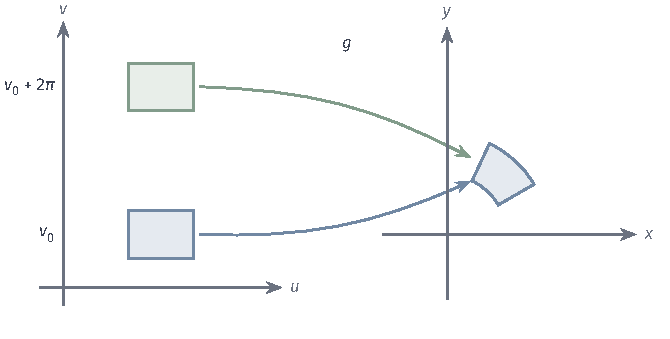
\includegraphics[width=112mm]{figures/02-vectors-matrices-and-multivariate-calculus/04-multivariate-calculus/tikz/explanation-additions/local-inverse-covering.pdf}
\caption{映射$g(u,v)=(e^u\cos v,e^u\sin v)$的重复覆盖。左侧蓝、绿矩形具有相同的$u$范围，$v$范围相差$2\pi$；右侧表示它们共同的扇环像。位置与宽度为示意，不按两边的坐标比例绘制。处处非奇异的Jacobian保证局部可逆，却不消除周期造成的整体多对一。}
\label{fig:v2-local-inverse-covering}
\end{figure}

另一方面，有连续的逆也不保证逆可微。一元函数$x\mapsto x^3$全局单射，其逆$y\mapsto y^{1/3}$在$0$处没有有限导数；这对应$x^3$在$0$处导数为零，定理条件不满足。所以Jacobian非奇异的条件不能由整体单射代替；使用局部反函数定理时，邻域、可微性和Jacobian的可逆性都要逐项检查。

第~\ref{chap:region-integrals}章用坐标变换计算区域积分时（第~\ref{sec:classical-change-variables}节），还须检查所用区域上的一一对应、光滑性和边界的处理，不能仅凭一点处Jacobian非零就对整个区域换元。

\FloatBarrier
\section{本章小结}
\label{sec:implicit-inverse-summary}

方程$F(\bm x,\bm y)=\bm0$在一点附近能否把$\bm y$解成$\bm x$的函数，取决于两件事：先指定一个起始解$(\bm a,\bm b)$，再检查关于待解变量的Jacobian$\bm D_{\bm y}F(\bm a,\bm b)$是否可逆。线性方程说明了这个条件的来源：系数方阵可逆时解唯一，否则解不存在或不唯一。隐函数定理断言，在$F$连续可微、该Jacobian可逆时，非线性方程在局部也有唯一的连续可微解分支，导数是$-(\bm D_{\bm y}F)^{-1}\bm D_{\bm x}F$。

证明把解方程改写为固定斜率的修正迭代，依次核对三件事：修正映射在一个闭球上是压缩，它不把球内的点送出球，所得不动点随参数Lipschitz并可微。存在与唯一是定理真正困难的部分；对恒等式$F(\bm x,\varphi(\bm x))=\bm0$形式求导，只能在分支已知可微时给出导数公式。

反函数定理是同一机制的特例：把$G(\bm x)-\bm y=\bm0$中的输出当作参数，$\bm J_G(\bm a)$可逆时，$G$在$\bm a$附近与$G(\bm a)$附近的开集之间可逆，逆映射的Jacobian是原Jacobian的逆。两类问题中，可逆的Jacobian都保证线性近似可以唯一地反解，从而局部的非线性问题也可以。

这些结论都是局部的。唯一性只限于所选邻域，远处可以有其他解支；Jacobian处处可逆的映射仍可能不是整体单射，例如$(u,v)\mapsto(e^u\cos v,e^u\sin v)$；Jacobian奇异时定理不作结论，既不能断言分支不存在，也不能默认它光滑。区域积分的换元还要另外检查整个区域上的一一对应。解分支的响应有多大、在有限扰动下一阶近似是否可靠，由下一章讨论。

\chapter{微分与扰动分析}
\label{chap:differential-perturbation-analysis}

测量误差、舍入误差或数据的轻微变化，都会让输入偏离理想值。第~\ref{chap:condition-and-spectral-perturbation}章已经不借助微分，直接比较精确变化$F(\bm x+\bm h)-F(\bm x)$，得到线性作用的条件数和谱的有限扰动界；这些界对一切方向取最坏情形。前三章则给出了另一种工具：微分把变化分成对$\bm h$线性的一阶响应和余项。本章把两者结合起来，回答三个问题：沿指定方向改变输入时，输出的一阶响应是什么；在所有允许方向中，误差最多被放大多少倍；对给定的有限步长，线性预测还差多少。

第一节对一般可微映射回答后两个问题。局部条件数用有限变化定义，可微时等于微分在允许方向子空间上的算子范数；余项界则需要导数沿整条扰动线段的变化，得到带明确常数的二次估计。这一节建立的是分析方法，不依赖具体运算。

后两节把这套方法用于矩阵。第二节调用第~\ref{chap:matrix-differentiation}章的微分公式与精确增量，逐个估计基本运算、求逆、行列式和对数行列式的一阶响应、条件数和余项，并检查整条扰动线段是否留在定义域内。第三节处理没有显式公式的输出：用第~\ref{chap:implicit-inverse-functions}章的隐函数定理证明简单特征值与特征向量的分支可微，计算它们沿指定方向的响应，并说明一阶近似何时可靠。

本章所用的有限扰动界都以第~\ref{chap:condition-and-spectral-perturbation}章为准，逆矩阵与方程解的完整误差分析以第~\ref{chap:solution-error-regularization}章为准。本章补充的是指定方向的一阶响应与它在有限步长下的精度，不重复那里的稳定性证明，也不评价求解算法。

\section{一般映射的扰动分析}
\label{sec:multivariable-differential-perturbation}

输入带有误差时，输出会偏离多少？第~\ref{chap:multivariate-differentiation}章的微分给出一阶预测：输入改变$\bm h$时，输出的变化约为$\mathrm dF_{\bm x}(\bm h)$。把精确变化写成
\[
 \Delta F=F(\bm x+\bm h)-F(\bm x)=\mathrm dF_{\bm x}(\bm h)+R_{\bm x}(\bm h),
\]
本节回答两个问题：在所有允许方向中，一阶误差最多被放大多少倍；对给定的有限步长，一阶预测还差多少。前一个问题由微分的算子范数回答，后一个问题需要控制导数沿扰动线段的变化。

本节的输入、输出空间都是有限维赋范空间，例如取某种范数的$\mathbb R^d$，或按元素排成坐标的矩阵空间。可微性的定义与$\mathbb R^d$中相同；由范数等价（定理~\ref{thm:ls-norm-equivalence}），可微与否不依赖所选范数，只有算子范数的数值依赖范数。

\subsection{局部条件数与导数范数}
\label{sec:multivariable-local-condition-number}

先回顾第~\ref{chap:condition-and-spectral-perturbation}章的结论。对固定矩阵的线性作用$\bm x\mapsto\bm A\bm x$，输出误差与输入误差之比只依赖扰动方向，在全部方向上取上确界，就得到放大倍数$\lVert\bm A\rVert$；相对误差的最坏放大不超过$\kappa(\bm A)=\lVert\bm A\rVert\lVert\bm A^{-1}\rVert$（第~\ref{sec:ls-perturbation-conditioning}节）。这些结论对任意大小的扰动都成立。

一般映射$F$不是线性的，误差比还随扰动大小改变，所以要先在半径为$\delta$的小扰动中取最坏情形，再让半径缩小。

固定基点$\bm x$与输入、输出空间的范数，并设$F$在$\bm x$的一个开邻域内有定义。若只允许对称扰动等结构化变化，就固定一个非零线性子空间$\mathcal E$作为允许的扰动方向，并只在$\bm x+\mathcal E$中取邻域；无结构限制时$\mathcal E$是整个输入空间。
\begin{definition}[局部条件数]
\label{def:multivariable-local-condition-number}
$F$在$\bm x$处相对于允许子空间$\mathcal E$的\term{局部条件数}（local condition number），也称局部绝对条件数，定义为
\begin{equation}
 \kappa_{\mathrm{abs}}(F,\bm x)=\lim_{\delta\downarrow0}\ \sup_{\bm h\in\mathcal E,\ 0<\lVert\bm h\rVert\leq\delta}\frac{\lVert F(\bm x+\bm h)-F(\bm x)\rVert}{\lVert\bm h\rVert}.
\label{eq:multivariable-local-condition-number}
\end{equation}
\end{definition}
内层的上确界覆盖全部允许方向，随$\delta$减小而不增，所以极限在$[0,\infty]$中存在。定义只用到函数值的有限变化，不要求$F$可微。它也不同于沿某个给定方向的响应：后者只是上确界中的一项，最坏方向上的放大可能大得多。

$F$可微时，局部条件数恰好是微分的算子范数。
\begin{theorem}[可微映射的局部条件数]
\label{thm:multivariable-local-condition-number}
若$F$在$\bm x$处可微，则
\begin{equation}
 \kappa_{\mathrm{abs}}(F,\bm x)=\max_{\bm h\in\mathcal E,\ \lVert\bm h\rVert=1}\lVert\mathrm dF_{\bm x}(\bm h)\rVert,
\label{eq:multivariable-local-condition-derivative-norm}
\end{equation}
即微分限制在允许子空间上的算子范数$\lVert\mathrm dF_{\bm x}|_{\mathcal E}\rVert$。
\end{theorem}
\begin{proof}
记余项$R_{\bm x}(\bm h)=F(\bm x+\bm h)-F(\bm x)-\mathrm dF_{\bm x}(\bm h)$，并令
\[
 \eta(\delta)=\sup_{\bm h\in\mathcal E,\ 0<\lVert\bm h\rVert\leq\delta}\frac{\lVert R_{\bm x}(\bm h)\rVert}{\lVert\bm h\rVert}.
\]
可微性说明$\bm h\to\bm0$时$\lVert R_{\bm x}(\bm h)\rVert/\lVert\bm h\rVert\to0$，按极限的定义，$\eta(\delta)\to0$。记$N=\lVert\mathrm dF_{\bm x}|_{\mathcal E}\rVert$。

一方面，由三角不等式，每个比值满足
\[
 \frac{\lVert F(\bm x+\bm h)-F(\bm x)\rVert}{\lVert\bm h\rVert}
 \leq\frac{\lVert\mathrm dF_{\bm x}(\bm h)\rVert}{\lVert\bm h\rVert}+\frac{\lVert R_{\bm x}(\bm h)\rVert}{\lVert\bm h\rVert}
 \leq N+\eta(\delta).
\]

另一方面，有限维线性映射的算子范数可以取到（第~\ref{sec:multivariable-operator-norm}节），取单位向量$\bm h_0\in\mathcal E$使$\lVert\mathrm dF_{\bm x}(\bm h_0)\rVert=N$，令$\bm h=\delta\bm h_0$；由反向三角不等式，
\[
 \frac{\lVert F(\bm x+\bm h)-F(\bm x)\rVert}{\lVert\bm h\rVert}
 \geq\frac{\lVert\mathrm dF_{\bm x}(\bm h)\rVert}{\lVert\bm h\rVert}-\frac{\lVert R_{\bm x}(\bm h)\rVert}{\lVert\bm h\rVert}
 \geq N-\eta(\delta).
\]
所以内层上确界介于$N-\eta(\delta)$与$N+\eta(\delta)$之间，令$\delta\downarrow0$即得。
\end{proof}
所以局部条件数就是最坏方向上的一阶敏感性。若只允许结构化扰动，微分和最坏方向都限制在允许的子空间内，所得数值一般不大于无结构的情形。

\paragraph{相对条件数}
输入、输出的参照量均非零时，把绝对条件数乘以输入尺度、除以输出尺度，得到相对条件数
\[
 \kappa_{\mathrm{rel}}(F,\bm x)=\kappa_{\mathrm{abs}}(F,\bm x)\,\frac{\lVert\bm x\rVert}{\lVert F(\bm x)\rVert},
\]
它衡量相对扰动在一阶上被放大多少倍。

对固定矩阵的线性作用$F(\bm x)=\bm A\bm x$，余项为零，误差比$\lVert\bm A\bm h\rVert/\lVert\bm h\rVert$与步长无关，局部绝对条件数就是$\lVert\bm A\rVert$，相对条件数是$\lVert\bm A\rVert\lVert\bm x\rVert/\lVert\bm A\bm x\rVert$。$\bm A$可逆时，
\[
 \lVert\bm x\rVert=\lVert\bm A^{-1}\bm A\bm x\rVert\leq\lVert\bm A^{-1}\rVert\lVert\bm A\bm x\rVert,
\]
代入后相对条件数不超过$\lVert\bm A\rVert\lVert\bm A^{-1}\rVert=\kappa(\bm A)$，这正回到第~\ref{sec:ls-perturbation-conditioning}节的精确结论。

这里有三个容易混淆的量。矩阵条件数$\kappa(\bm A)$对全部输入取最坏情形，是固定线性作用的统一上界；固定输入$\bm x$处的相对条件数只涉及这一点；把矩阵本身当作输入时，某个矩阵映射（例如求逆）的条件数又是另一个问题，第~\ref{sec:multivariable-matrix-operation-perturbation}节将具体计算。它们描述的都是数学问题本身对输入变化的敏感性；问题条件数与求解算法稳定性的分工见第~\ref{sec:ls-numerical-stability}节，二者不能互相代替。

\paragraph{有限条件数而不可微}
条件数有限并不要求可微。取实对称矩阵$\bm S(t)=\operatorname{diag}(t,-t)$，把$t\in\mathbb R$作为标量输入，输出取排序后的最大特征值$\lambda_{\max}(\bm S(t))=|t|$，两端都用绝对值度量。由Weyl界（定理~\ref{thm:ls-weyl-eigenvalue}），
\[
 |\lambda_{\max}(\bm S(t))-\lambda_{\max}(\bm S(s))|\leq\lVert\bm S(t)-\bm S(s)\rVert_2=|t-s|,
\]
有限变化受到控制；在$t=0$处，比值$|\lambda_{\max}(\bm S(h))-0|/|h|$恒为$1$，所以局部绝对条件数为$1$。

可是$|t|$在$0$处没有双侧导数，这个条件数不能用微分的范数解释。失去可微性的是“排序后取最大”这一步：两条未排序的特征值分支$t$与$-t$本身光滑，它们在$t=0$相交，最大值在交点处从一支换到另一支。第~\ref{sec:multivariable-eigen-differential}节将在特征值简单的条件下，证明所选的局部分支可微。


图~\ref{fig:v2-ordered-eigenvalue-kink}把两条光滑分支与排序后的包络分开画出，可以看见不可微性来自交点处的分支切换。
\begin{figure}[!htb]
\centering
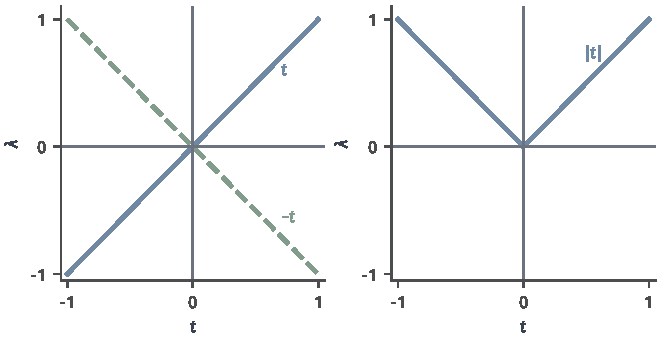
\includegraphics[width=112mm]{figures/02-vectors-matrices-and-multivariate-calculus/04-multivariate-calculus/matplotlib/explanation-additions/ordered-eigenvalue-kink.pdf}
\caption{$\bm S(t)=\operatorname{diag}(t,-t)$。左图为未排序分支$t$与$-t$，右图为最大特征值$|t|$。两侧斜率在零点不同，但函数仍为$1$-Lipschitz，零点的局部绝对条件数仍为$1$。}
\label{fig:v2-ordered-eigenvalue-kink}
\end{figure}

反过来，局部条件数为零也不说明输出不变。$f(t)=t^2$在$0$处导数为零，局部条件数为$0$，但有限步长$t$仍带来变化$t^2$。一阶分析在这里预测“没有变化”，被遗漏的部分要由下一小节的余项界估计。

\subsection{一阶近似的余项界}
\label{sec:multivariable-first-order-remainder}

可微性只保证余项是$o(\lVert\bm h\rVert)$，并不给出某个有限扰动的数值误差界。要得到这样的界，需要知道导数沿扰动线段怎样变化。本小节输入、输出都取欧氏范数，矩阵空间取Frobenius范数，即拉直后的欧氏范数；导数的大小用谱范数度量。其他范数下可借范数等价改变常数。

设$F$在包含线段$[\bm x,\bm x+\bm h]$的开集上连续可微。式~\eqref{eq:multivariable-vector-integral-increment}给出完整增量$\int_0^1\bm J_F(\bm x+t\bm h)\bm h\,\mathrm dt$；从中扣除常向量$\bm J_F(\bm x)\bm h=\int_0^1\bm J_F(\bm x)\bm h\,\mathrm dt$，得到余项的精确表示
\begin{equation}
 R_{\bm x}(\bm h)=F(\bm x+\bm h)-F(\bm x)-\bm J_F(\bm x)\bm h
 =\int_0^1\bigl(\bm J_F(\bm x+t\bm h)-\bm J_F(\bm x)\bigr)\bm h\,\mathrm dt .
\label{eq:multivariable-remainder-integral}
\end{equation}
对照两种估计：完整增量由沿线段的导数大小$\lVert\bm J_F\rVert_2$控制（式~\eqref{eq:analysis-operator-mean-value-bound}），余项则由导数相对基点的变化$\lVert\bm J_F(\bm x+t\bm h)-\bm J_F(\bm x)\rVert_2$控制。导数很大而变化很慢时，整个增量可以很大，一阶预测却仍然准确；二者估计的是不同对象。
\begin{theorem}[一阶近似的二次余项界]
\label{thm:multivariable-first-order-remainder-bound}
设$F$在包含线段$[\bm x,\bm x+\bm h]$的开集上连续可微，且存在常数$L\geq0$，使
\[
 \lVert\bm J_F(\bm y)-\bm J_F(\bm x)\rVert_2\leq L\lVert\bm y-\bm x\rVert_2\qquad(\bm y\in[\bm x,\bm x+\bm h]).
\]
则
\begin{equation}
 \lVert F(\bm x+\bm h)-F(\bm x)-\bm J_F(\bm x)\bm h\rVert_2\leq\frac L2\lVert\bm h\rVert_2^2 .
\label{eq:multivariable-first-order-remainder-bound}
\end{equation}
\end{theorem}
\begin{proof}
取$\bm y=\bm x+t\bm h$，假设给出
\[
 \lVert\bm J_F(\bm x+t\bm h)-\bm J_F(\bm x)\rVert_2\leq Lt\lVert\bm h\rVert_2 .
\]
对式~\eqref{eq:multivariable-remainder-integral}使用向量积分的范数不等式与谱范数的界，
\[
 \lVert R_{\bm x}(\bm h)\rVert_2
 \leq\int_0^1\bigl\lVert\bigl(\bm J_F(\bm x+t\bm h)-\bm J_F(\bm x)\bigr)\bm h\bigr\rVert_2\,\mathrm dt
 \leq\int_0^1Lt\lVert\bm h\rVert_2^2\,\mathrm dt=\frac L2\lVert\bm h\rVert_2^2 .
\]
\end{proof}
定理只要求一阶导数相对基点满足Lipschitz型的界，不以Hessian或二阶导数的存在为前提。若$\bm J_F$在一个凸邻域内以$L$为Lipschitz常数，邻域内每条线段都满足假设。定理~\ref{thm:multivariable-second-derivative-lipschitz}已说明，$F\in C^2$时二阶导数的统一界$M$就是这样的常数，于是余项不超过$M\lVert\bm h\rVert_2^2/2$；这是取得该条件的一种充分办法。

上界正比于$\lVert\bm h\rVert_2^2$：步长缩小到一半，上界缩小到四分之一。这说明的是所保证误差的量级，并不意味着实际误差恰好按同样比例变化，实际误差也可能远小于上界。

例如对称二次型$q(\bm x)=\bm x^\top\bm S\bm x$的Jacobian是$\nabla q^\top=2\bm x^\top\bm S$，满足
\[
 \lVert2\bm S\bm y-2\bm S\bm x\rVert_2\leq2\lVert\bm S\rVert_2\lVert\bm y-\bm x\rVert_2 ;
\]
定理给出余项界$\lVert\bm S\rVert_2\lVert\bm h\rVert_2^2$，与第~\ref{sec:multivariable-differential-rules}节由精确增量得到的$|\bm h^\top\bm S\bm h|\leq\lVert\bm S\rVert_2\lVert\bm h\rVert_2^2$一致。

\paragraph{三种保证的分工}
可微给出统一的$o(\lVert\bm h\rVert)$，只说明步长趋零时的行为；导数的Lipschitz界给出带明确常数的二次余项；第~\ref{sec:multivariable-vector-increment-bound}节的导数界则控制整个有限变化。

使用后两者之前都要先检查：扰动线段是否留在定义域内，可逆、正定等结构条件是否在整条线段上保持，所需常数是否在这个范围内统一成立。矩阵映射的这些检查可以借助已有的有限扰动结论：第~\ref{chap:condition-and-spectral-perturbation}章的Weyl界与奇异值扰动界判断正定性与可逆性是否保持，第~\ref{sec:ls-inverse-sensitivity}节的逆矩阵有限界控制求逆在整段上的变化。基点的条件数只描述无穷小扰动，不能代替这些范围检查和余项估计；下一节对各种矩阵运算逐一完成这些检查。

\section{矩阵运算的扰动分析}
\label{sec:multivariable-matrix-operation-perturbation}

第~\ref{chap:matrix-differentiation}章已经求出常用矩阵运算的微分，并用增量的一阶项验证了可微性。本节回到误差问题：矩阵数据带有扰动$\bm E$时，这些微分给出的线性预测在有限步长下有多准，误差在最坏方向上被放大多少。

对每种运算都要同时检查三件事：输出是矩阵还是标量，因而误差用什么范数或尺度度量；扰动是否受对称等结构限制；整条扰动线段是否留在定义域内。前一节的一般原则在这里落到具体的余项表达式上。本节的矩阵范数除特别说明外取满足乘积不等式$\lVert\bm X\bm Y\rVert\leq\lVert\bm X\rVert\lVert\bm Y\rVert$的范数，例如谱范数或Frobenius范数；求逆时取由向量范数诱导的矩阵范数，它还满足$\lVert\bm I\rVert=1$。

\subsection{基本矩阵运算的增量与余项}
\label{sec:multivariable-basic-operation-remainder}

第~\ref{sec:multivariable-matrix-basic-operations}节对转置、乘法、平方、迹、Frobenius范数平方和二次型写出了精确增量。这些增量都是扰动的多项式，所以余项不必另行估计，直接从增量中读出，再用范数控制大小。

\paragraph{线性运算}
加法、数乘、转置、迹以及$\bm X\mapsto\bm A\bm X\bm B$都是线性映射，精确增量就是一阶项，余项恒为零。对这些运算，线性预测在任意步长下都精确，误差问题只剩放大倍数。由定理~\ref{thm:multivariable-local-condition-number}，局部绝对条件数就是运算本身的算子范数，且与基点无关。

例如在Frobenius范数下，转置不改变任何矩阵的长度，条件数为$1$。迹则不同：由Cauchy--Schwarz不等式，
\[
 |\operatorname{tr}\bm E|=|\langle\bm I,\bm E\rangle_F|\leq\sqrt d\,\lVert\bm E\rVert_F ,
\]
取$\bm E=\bm I/\sqrt d$时等号成立，所以$d\times d$矩阵的迹的条件数为$\sqrt d$。各对角元的误差同号时会累加起来。

\paragraph{乘积与平方}
由式~\eqref{eq:multivariable-product-increment}，两个因子同时扰动时，
\[
 (\bm A+\bm E)(\bm B+\bm H)-\bm A\bm B-(\bm A\bm H+\bm E\bm B)=\bm E\bm H .
\]
由乘积不等式，一阶项与余项分别满足
\[
 \begin{gathered}
 \lVert\bm A\bm H+\bm E\bm B\rVert\leq\lVert\bm A\rVert\lVert\bm H\rVert+\lVert\bm E\rVert\lVert\bm B\rVert,\\
 \lVert\bm E\bm H\rVert\leq\lVert\bm E\rVert\lVert\bm H\rVert .
 \end{gathered}
\]
两者的比较说明：两个扰动都不超过$\rho$时，一阶项至多与$\rho$同阶，余项至多是$\rho^2$。

平方映射同理，$(\bm X+\bm E)^2-\bm X^2$的一阶项为$\bm X\bm E+\bm E\bm X$，余项恰为$\bm E^2$，且$\lVert\bm E^2\rVert\leq\lVert\bm E\rVert^2$。

这些界可以直接用作误差预算。若要求线性预测的绝对误差不超过$\tau$，乘积情形只需$\lVert\bm E\rVert\lVert\bm H\rVert\leq\tau$，两个扰动同样大小时步长不超过$\sqrt\tau$即可。若要求余项不超过一阶项的某个比例，则还要知道一阶项在所取方向上有多大，不能只看扰动的大小。
\begin{example}[矩阵平方的一阶预测]
\label{ex:multivariable-square-first-order-check}
取$\bm X=\operatorname{diag}(2,1)$与扰动$\bm E=\varepsilon\bm K$，其中
\[
 \bm K=\begin{bmatrix}0&1\\1&0\end{bmatrix}.
\]
一阶项与余项分别为
\[
 \bm X\bm E+\bm E\bm X=\varepsilon\begin{bmatrix}0&3\\3&0\end{bmatrix},\qquad
 \bm E^2=\varepsilon^2\bm I ,
\]
谱范数分别为$3\varepsilon$与$\varepsilon^2$。取$\varepsilon=0.1$，一阶项为$0.3$，余项为$0.01$，约为一阶项的$3\%$。

若要求余项不超过一阶项的$1\%$，需要
\[
 \frac{\varepsilon^2}{3\varepsilon}\leq0.01 ,
\]
即扰动须满足$\varepsilon\leq0.03$。
\end{example}

\paragraph{Frobenius范数平方与二次型}
标量输出的运算同样可以读出余项。Frobenius范数平方的精确增量为
\[
 \lVert\bm X+\bm E\rVert_F^2-\lVert\bm X\rVert_F^2=2\langle\bm X,\bm E\rangle_F+\lVert\bm E\rVert_F^2 ,
\]
余项恰为$\lVert\bm E\rVert_F^2$，与方向无关。一阶项$2\langle\bm X,\bm E\rangle_F$却可能为零：扰动与$\bm X$正交时，线性预测说“没有变化”，实际变化却是$\lVert\bm E\rVert_F^2$。这时余项与一阶项之比没有意义，应直接给出绝对误差的预算。

二次型$\bm x^\top\bm A\bm x$在$\bm A$与$\bm x$同时扰动时，第~\ref{sec:multivariable-matrix-basic-operations}节写出的余项为
\[
 \bm h^\top\bm A\bm h+\bm x^\top\bm E\bm h+\bm h^\top\bm E\bm x+\bm h^\top\bm E\bm h .
\]
在谱范数下，它的绝对值不超过
\[
 \lVert\bm A\rVert_2\lVert\bm h\rVert_2^2+2\lVert\bm E\rVert_2\lVert\bm x\rVert_2\lVert\bm h\rVert_2+\lVert\bm E\rVert_2\lVert\bm h\rVert_2^2 .
\]
每一项都含两个扰动因子，其中$\lVert\bm E\rVert_2\lVert\bm h\rVert_2$一项还乘了基点的大小$\lVert\bm x\rVert_2$：基点越大，矩阵与向量扰动的交叉作用越强。

比较起来，线性运算的余项为零，多项式运算的余项是扰动的二次或更高次项，并且可以精确写出。误差预算由这些高次项决定线性预测可用的步长；导数本身的大小只决定一阶项，不决定预测还差多少。

\subsection{求逆的扰动}
\label{sec:multivariable-inverse-perturbation}

第~\ref{sec:multivariable-inverse-differential}节由逆差恒等式证明了求逆可微，并得到$\mathrm d(\bm X^{-1})=-\bm X^{-1}\mathrm d\bm X\bm X^{-1}$。那里只用到余项是$o(\lVert\bm E\rVert)$。本节把余项精确写出，给出它的二次界，再计算求逆的条件数，并说明它与线性方程解映射的联系。

\paragraph{精确余项与可逆邻域}
设$\bm A$可逆，$\bm B=\bm A+\bm E$，$q=\lVert\bm A^{-1}\rVert\lVert\bm E\rVert<1$。由逆差恒等式~\eqref{eq:ch06-inverse-finite-perturbation}，
\[
 \bm B^{-1}-\bm A^{-1}=-\bm B^{-1}\bm E\bm A^{-1}.
\]
把右端的$\bm B^{-1}$写成$\bm A^{-1}+(\bm B^{-1}-\bm A^{-1})$，再用一次同一恒等式，
\[
 \bm B^{-1}-\bm A^{-1}
 =-\bm A^{-1}\bm E\bm A^{-1}-(\bm B^{-1}-\bm A^{-1})\bm E\bm A^{-1}
 =-\bm A^{-1}\bm E\bm A^{-1}+\bm B^{-1}\bm E\bm A^{-1}\bm E\bm A^{-1}.
\]
第一项是一阶预测，第二项是精确余项。由$\lVert\bm B^{-1}\rVert\leq\lVert\bm A^{-1}\rVert/(1-q)$（第~\ref{sec:ls-inverse-sensitivity}节），
\begin{equation}
 \lVert\bm B^{-1}\bm E\bm A^{-1}\bm E\bm A^{-1}\rVert
 \leq\lVert\bm B^{-1}\rVert\lVert\bm A^{-1}\rVert^2\lVert\bm E\rVert^2
 \leq\frac{\lVert\bm A^{-1}\rVert^3\lVert\bm E\rVert^2}{1-q}.
\label{eq:multivariable-inverse-remainder-bound}
\end{equation}

第~\ref{chap:linear-recurrence-stability}章的Neumann级数给出同一结论的另一种看法。写$\bm B=\bm A(\bm I-\bm T)$，其中$\bm T=-\bm A^{-1}\bm E$，$\lVert\bm T\rVert\leq q<1$，因而谱半径小于$1$。由定理~\ref{thm:ls-neumann}，$\bm I-\bm T$可逆，且
\[
 \bm B^{-1}=\sum_{k\geq0}\bm T^k\bm A^{-1}.
\]
前两项$\bm A^{-1}-\bm A^{-1}\bm E\bm A^{-1}$正是一阶预测；截断误差界~\eqref{eq:ls-neumann-tail}取$N=1$，给出余项不超过$q^2\lVert\bm A^{-1}\rVert/(1-q)$，与式~\eqref{eq:multivariable-inverse-remainder-bound}相同。级数还说明，余项依次由$\bm E$的二次、三次……项组成。

\paragraph{一阶预测的误差}
式~\eqref{eq:multivariable-inverse-remainder-bound}同时是有限扰动下一阶预测的误差界。对$0\leq t\leq1$，$\lVert\bm A^{-1}(t\bm E)\rVert\leq tq<1$，所以整条扰动线段$\bm A+t\bm E$都由可逆矩阵组成，定义域条件在整段上成立。

于是可以比较三个量：实际逆矩阵$(\bm A+\bm E)^{-1}$，一阶预测$\bm A^{-1}-\bm A^{-1}\bm E\bm A^{-1}$，以及二者之差。第~\ref{sec:ls-inverse-sensitivity}节控制的是全变化，
\[
 \lVert(\bm A+\bm E)^{-1}-\bm A^{-1}\rVert\leq\frac{\lVert\bm A^{-1}\rVert^2\lVert\bm E\rVert}{1-q},
\]
与$\lVert\bm E\rVert$同阶；本段新增的是从全变化中扣除一阶项之后，近似还差多少，它与$\lVert\bm E\rVert^2$同阶。$q$接近$1$时两种界都变得很大，一阶预测不再可靠。
\begin{example}[逆矩阵的一阶预测与余项]
\label{ex:multivariable-inverse-first-order-check}
取$\bm A=\operatorname{diag}(2,1)$与扰动
\[
 \bm E=\begin{bmatrix}0&0.1\\0.1&0\end{bmatrix},
\]
采用谱范数，则$\lVert\bm A^{-1}\rVert_2=1$、$\lVert\bm E\rVert_2=0.1$、$q=0.1$。这个矩阵可以直接求逆，
\[
 (\bm A+\bm E)^{-1}=\frac1{1.99}\begin{bmatrix}1&-0.1\\-0.1&2\end{bmatrix},
\]
而一阶预测为
\[
 \bm A^{-1}-\bm A^{-1}\bm E\bm A^{-1}=\begin{bmatrix}0.5&-0.05\\-0.05&1\end{bmatrix}.
\]
实际值减去预测，剩下的余项为
\[
 \frac{0.0005}{1.99}\begin{bmatrix}10&-1\\-1&20\end{bmatrix}\approx\begin{bmatrix}0.00251&-0.00025\\-0.00025&0.00503\end{bmatrix}.
\]

现在比较几个量的大小。余项的谱范数约为$0.00505$，约为一阶项谱范数$0.05$的十分之一，并落在式~\eqref{eq:multivariable-inverse-remainder-bound}的上界$0.01/0.9\approx0.0111$之内。

再看全变化。全变化$(\bm A+\bm E)^{-1}-\bm A^{-1}$的谱范数约为$0.0540$，第~\ref{sec:ls-inverse-sensitivity}节的全变化界为$0.1/0.9\approx0.111$。
\end{example}
一阶预测扣除了全变化中约$0.05$的主要部分，剩下的误差约为扰动大小的平方量级；余项界比实际误差大约两倍，它只保证误差不超过多少。

\paragraph{求逆的条件数}
在无结构限制的扰动模型下，输入、输出都取谱范数。由乘积不等式，
\[
 \lVert\bm A^{-1}\bm E\bm A^{-1}\rVert_2\leq\lVert\bm A^{-1}\rVert_2^2\lVert\bm E\rVert_2 .
\]

这个上界可以取到。设$\sigma_d$是$\bm A$的最小奇异值，对应的左、右奇异向量为$\bm u_d,\bm v_d$，即$\bm A\bm v_d=\sigma_d\bm u_d$、$\bm A^\top\bm u_d=\sigma_d\bm v_d$（第~\ref{sec:ls-svd}章）。取$\bm E=\bm u_d\bm v_d^\top$，它的谱范数为$1$。由$\bm A^{-1}\bm u_d=\bm v_d/\sigma_d$与$\bm A^{-\top}\bm v_d=\bm u_d/\sigma_d$，
\[
 \bm A^{-1}\bm E\bm A^{-1}=(\bm A^{-1}\bm u_d)(\bm A^{-\top}\bm v_d)^\top=\frac{\bm v_d\bm u_d^\top}{\sigma_d^2},
\]
其谱范数为$1/\sigma_d^2=\lVert\bm A^{-1}\rVert_2^2$。

由定理~\ref{thm:multivariable-local-condition-number}，求逆映射在$\bm A$处的局部绝对条件数为$\lVert\bm A^{-1}\rVert_2^2$，相对条件数为
\[
 \lVert\bm A^{-1}\rVert_2^2\cdot\frac{\lVert\bm A\rVert_2}{\lVert\bm A^{-1}\rVert_2}=\lVert\bm A\rVert_2\lVert\bm A^{-1}\rVert_2=\kappa_2(\bm A).
\]

矩阵条件数在这里重新出现，但含义不同：这里输入是矩阵本身，输出是逆矩阵，而第~\ref{sec:ls-matrix-condition-number}节的输入是向量。若限制扰动结构，例如只允许对称扰动，须改用微分在允许子空间上的范数。求解方程的算法及其数值稳定性仍按第~\ref{chap:solution-error-regularization}章处理。

\paragraph{线性方程的解映射}
求逆与乘法复合，得到线性方程的解映射
\[
 \operatorname{sol}(\bm A,\bm b)=\bm A^{-1}\bm b ,
\]
它定义在可逆$\bm A$与任意$\bm b$组成的开集上。固定可逆的$\bm A$，记$\bm x=\bm A^{-1}\bm b$；联合输入$(\bm E,\bm f)$取乘积范数$\lVert(\bm E,\bm f)\rVert=(\lVert\bm E\rVert^2+\lVert\bm f\rVert^2)^{1/2}$，其中$\bm f$是右端的增量。

第~\ref{sec:ls-equation-sensitivity}节从扰动后的方程
\[
 (\bm A+\bm E)(\bm x+\Delta\bm x)=\bm b+\bm f
\]
中减去$\bm A\bm x=\bm b$，得到
\[
 (\bm A+\bm E)\Delta\bm x=\bm f-\bm E\bm x .
\]
在$q<1$时，这给出精确式
\[
 \Delta\bm x=(\bm A+\bm E)^{-1}(\bm f-\bm E\bm x).
\]
把$(\bm A+\bm E)^{-1}$拆成$\bm A^{-1}$与逆差，
\[
 \Delta\bm x=\bm A^{-1}(\bm f-\bm E\bm x)+\bigl((\bm A+\bm E)^{-1}-\bm A^{-1}\bigr)(\bm f-\bm E\bm x).
\]
第一项对$(\bm E,\bm f)$线性。第二项中，两个因子分别满足
\[
 \begin{gathered}
 \bigl\lVert(\bm A+\bm E)^{-1}-\bm A^{-1}\bigr\rVert\leq\frac{\lVert\bm A^{-1}\rVert^2\lVert\bm E\rVert}{1-q},\\
 \lVert\bm f-\bm E\bm x\rVert\leq\lVert\bm f\rVert+\lVert\bm E\rVert\lVert\bm x\rVert ;
 \end{gathered}
\]
二者都不超过联合扰动大小的常数倍，所以第二项是联合扰动的二次量。因此解映射可微，且
\begin{equation}
 \mathrm d\operatorname{sol}_{(\bm A,\bm b)}(\bm E,\bm f)=\bm A^{-1}(\bm f-\bm E\bm x).
\label{eq:multivariable-solution-map-differential}
\end{equation}
也可以用链式法则核对：$\operatorname{sol}$是求逆与矩阵—向量乘法的复合，由乘积的联合微分与式~\eqref{eq:analysis-inverse-differential}，一阶项为
\[
 (-\bm A^{-1}\bm E\bm A^{-1})\bm b+\bm A^{-1}\bm f=\bm A^{-1}(\bm f-\bm E\bm x),
\]
结果相同。第~\ref{sec:multivariable-implicit-function}节已用隐函数公式核对过同一结果。

第~\ref{sec:ls-equation-sensitivity}节的界控制完整的解误差，式~\eqref{eq:multivariable-solution-map-differential}则提取局部的一阶预测，上面的拆分还说明预测的误差是联合扰动的二次量。数据误差、残差与算法稳定性的完整分析仍以第~\ref{chap:solution-error-regularization}章为准，本节只补充一阶响应及其精度。

\subsection{行列式的扰动}
\label{sec:multivariable-determinant-perturbation}

第~\ref{sec:multivariable-determinant-differential}节逐列展开$\det(\bm A+\bm E)$，得到一阶项$\langle\bm C,\bm E\rangle_F$，其中$\bm C$是代数余子式矩阵；展开中其余各项至少含两列扰动。这些高阶项就是线性预测的误差。它们对包括奇异矩阵在内的全部方阵都有意义，所以先讨论绝对误差，再在可逆时讨论相对误差。

\paragraph{绝对变化的余项}
在固定的有界邻域内，余项有二次控制。记$K=\{\bm A+\bm F:\lVert\bm F\rVert_F\leq1\}$。行列式的二阶偏导数都是多项式，在闭有界集$K$上有界，所以存在$M$使$\lVert D^2\det_{\bm Z}\rVert\leq M$对$\bm Z\in K$成立。

对$\lVert\bm E\rVert_F\leq1$，令$g(t)=\det(\bm A+t\bm E)$，它是$t$的多项式。它的二阶导数及其界为
\[
 g''(t)=D^2\det_{\bm A+t\bm E}[\bm E,\bm E],\qquad |g''(t)|\leq M\lVert\bm E\rVert_F^2 .
\]
一元Taylor公式给出
\[
 \bigl|\det(\bm A+\bm E)-\det\bm A-\langle\bm C,\bm E\rangle_F\bigr|\leq\frac M2\lVert\bm E\rVert_F^2 ,
\]
常数$M$依赖所取的邻域。

二阶情形可以精确写出余项。对$\bm A,\bm E\in\mathbb R^{2\times2}$，直接展开得
\[
 \det(\bm A+\bm E)=\det\bm A+\langle\bm C,\bm E\rangle_F+\det\bm E ,
\]
余项就是$\det\bm E=E_{1,1}E_{2,2}-E_{1,2}E_{2,1}$。由$|ab|\leq(a^2+b^2)/2$，
\[
 |\det\bm E|\leq\frac{\lVert\bm E\rVert_F^2}2 ,
\]
即上式中可取$M=1$，而且这个界与基点$\bm A$无关，奇异的$\bm A$也适用。

\paragraph{条件数与相对变化}
对给定扰动方向，一阶响应是$\langle\bm C,\bm E\rangle_F$。由定理~\ref{thm:multivariable-local-condition-number}，局部绝对条件数是这个线性泛函在所选输入范数下的大小，即第~\ref{sec:ls-dual-norms}节的对偶范数：
\[
 \kappa_{\mathrm{abs}}(\det,\bm A)=\max_{\lVert\bm E\rVert\leq1}|\langle\bm C,\bm E\rangle_F| .
\]
输入取Frobenius范数时，由Cauchy--Schwarz不等式，$\bm C\neq\bm0$时最大值在$\bm E=\bm C/\lVert\bm C\rVert_F$处取到，所以$\kappa_{\mathrm{abs}}=\lVert\bm C\rVert_F$，可以直接由代数余子式算出。

可逆时还可以比较相对变化：由$\bm C=\det(\bm A)\bm A^{-\top}$，
\[
 \kappa_{\mathrm{rel}}(\det,\bm A)=\lVert\bm C\rVert_F\frac{\lVert\bm A\rVert_F}{|\det\bm A|}=\lVert\bm A^{-1}\rVert_F\lVert\bm A\rVert_F .
\]
奇异点处$\det\bm A=0$，只有绝对变化有定义，不能除以零行列式。

在相对尺度下，行列式对矩阵变化的反应可以远比矩阵本身的变化剧烈。
\begin{example}[接近奇异时的行列式]
\label{ex:ls-determinant-near-singular}
设$\bm A=\operatorname{diag}(1,\varepsilon)$，$0<\varepsilon<1$，它的行列式$\det\bm A=\varepsilon$很小。只改动第二个对角元，取扰动$\bm E=\operatorname{diag}(0,\delta)$，使它变为$\varepsilon+\delta$。矩阵采用谱范数、标量采用绝对值时，矩阵的相对变化为$\lVert\bm E\rVert_2/\lVert\bm A\rVert_2=|\delta|$；行列式则变为$\varepsilon+\delta$，相对变化为
\[
 \frac{|(\varepsilon+\delta)-\varepsilon|}{\varepsilon}=\frac{|\delta|}{\varepsilon}.
\]
用微分公式计算也得到同样的增量：
\[
 \det(\bm A)\operatorname{tr}(\bm A^{-1}\bm E)=\varepsilon\cdot\frac\delta\varepsilon=\delta .
\]
沿这个方向，行列式是$\delta$的一次函数，所以一阶预测没有余项。

两相比较，行列式的相对变化是矩阵相对变化的$1/\varepsilon$倍。$\varepsilon$越小，矩阵越接近奇异，沿这个方向的相对放大就越强。
\end{example}

但不能仅凭行列式的数值判断求逆是否病态。取$\bm A=\varepsilon\bm I\in\mathbb R^{d\times d}$（$\varepsilon>0$），行列式$\varepsilon^d$可以极小，而由第~\ref{sec:multivariable-inverse-perturbation}节，求逆的相对条件数是$\kappa_2(\varepsilon\bm I)=1$；行列式本身的相对条件数$\lVert\bm A^{-1}\rVert_F\lVert\bm A\rVert_F=d$也不随$\varepsilon$变大。行列式与逆矩阵是两个不同的输出，绝对与相对又是两种尺度，必须分别判断。

\subsection{对数行列式的扰动}
\label{sec:multivariable-logdet-perturbation}

由第~\ref{sec:multivariable-logdet-differential}节，$\log\det$在$\det>0$的开集上可微，微分为$\bm E\mapsto\operatorname{tr}(\bm A^{-1}\bm E)$。它给出一阶变化：
\[
 \log\det(\bm A+\bm E)-\log\det\bm A
 =\operatorname{tr}(\bm A^{-1}\bm E)+o(\lVert\bm E\rVert_F).
\]
相应的局部绝对条件数是线性泛函$\bm E\mapsto\langle\bm A^{-\top},\bm E\rangle_F$在所选输入范数下的对偶范数，Frobenius范数下为$\lVert\bm A^{-1}\rVert_F$。对数行列式可以为零或接近零，这时以它为分母的相对误差没有意义，应直接比较绝对变化。

\paragraph{整条线段的定义域}
要把一阶预测用于有限扰动，先要保证整条线段$\bm A+t\bm E$（$0\leq t\leq1$）留在定义域内。一般的正行列式矩阵，由行列式的连续性，总可以选足够小的邻域，使整条线段$\bm A+t\bm E$仍满足$\det>0$，但这不给出邻域的具体大小。正定情形则可以用第~\ref{chap:condition-and-spectral-perturbation}章的最小特征值界明确检查整条线段保持正定，下面的余项界就基于这一检查。

\paragraph{二次余项界}
设$\bm A$对称正定，最小特征值为$m>0$，$\bm E$对称且$\lVert\bm E\rVert_2<m$。对任意单位向量$\bm x$和$0\leq t\leq1$，
\[
 \bm x^\top(\bm A+t\bm E)\bm x\geq m-\lVert\bm E\rVert_2>0 ,
\]
所以整条线段保持正定，而且最小特征值有统一的正下界。

令$g(t)=\log\det(\bm A+t\bm E)$。由式~\eqref{eq:analysis-logdet-gradient}与链式法则，
\[
 g'(t)=\operatorname{tr}\bigl((\bm A+t\bm E)^{-1}\bm E\bigr);
\]
再用沿参数曲线的求逆公式，
\[
 g''(t)=-\operatorname{tr}\!\left((\bm A+t\bm E)^{-1}\bm E
 (\bm A+t\bm E)^{-1}\bm E\right).
\]
逆矩阵的谱范数至多为$(m-\lVert\bm E\rVert_2)^{-1}$。由Frobenius内积的Cauchy--Schwarz不等式与混合乘积界~\eqref{eq:matrix-analysis-mixed-submultiplicativity}，
\[
 |g''(t)|\leq\lVert(\bm A+t\bm E)^{-1}\bm E\rVert_F^2\leq\frac{\lVert\bm E\rVert_F^2}{(m-\lVert\bm E\rVert_2)^2}.
\]
于是一元Taylor公式给出
\begin{equation}
 \left|\log\det(\bm A+\bm E)-\log\det\bm A
 -\operatorname{tr}(\bm A^{-1}\bm E)\right|
 \leq\frac{\lVert\bm E\rVert_F^2}{2(m-\lVert\bm E\rVert_2)^2}.
\label{eq:multivariable-logdet-remainder-bound}
\end{equation}

例如$\bm A=\operatorname{diag}(2,1)$，$\bm E=\operatorname{diag}(0.1,0)$时，一阶预测为$0.05$，实际变化为$\log(1.05)\approx0.04879$。此时$m=1$，上述上界约为$0.00618$，大于实际误差约$0.00121$。这个界只保证误差不超过多少，不表示误差会接近上界。

导数给出变化的方向与大小，正定线段给出估计的有效范围，余项界说明预测的可靠程度，三者要一起使用。正定条件是这一显式估计的条件，不是一般正行列式矩阵上$\log\det$的定义条件。

上界的分母$m-\lVert\bm E\rVert_2$是扰动后最小特征值的保底下界，即到奇异边界的余量。$\bm A$接近奇异时，$m$很小：一阶响应的条件数$\lVert\bm A^{-1}\rVert_F\geq1/m$变大，余项界又按$1/(m-\lVert\bm E\rVert_2)^2$放大，允许的步长必须小于$m$。

例如$\bm A=\operatorname{diag}(1,\varepsilon)$、$\bm E=\operatorname{diag}(0,\delta)$时，精确变化是$\log(1+\delta/\varepsilon)$，一阶预测是$\delta/\varepsilon$；$\delta$与$\varepsilon$同阶时两者相差显著，$\delta\to-\varepsilon$时精确值趋于$-\infty$。

\section{特征值与特征向量的微分}
\label{sec:multivariable-eigen-differential}

特征值和特征向量由方程$\bm S\bm v=\lambda\bm v$确定，并不是矩阵元素的显式函数，前一节的显式计算不能直接使用。第~\ref{chap:condition-and-spectral-perturbation}章已经给出有限扰动下的稳定性界：对称扰动$\bm E$使每个排序后的特征值至多移动$\lVert\bm E\rVert_2$（Weyl界，定理~\ref{thm:ls-weyl-eigenvalue}），特征子空间的偏转受$\lVert\bm E\rVert_2$与谱隙之比控制（第~\ref{sec:ls-subspace-sensitivity}节）。这些界对一切方向取最坏情形。

本节回答另一个问题：沿一个指定的扰动方向，特征值与特征向量以什么速率变化，这个变化率在多大范围内可以用来预测。先用第~\ref{chap:implicit-inverse-functions}章的隐函数定理证明简单特征值所在的分支可微，再分别计算特征值与特征向量的微分，最后说明一阶近似的适用条件。

\subsection{特征值与特征向量的可微性}
\label{sec:multivariable-eigen-differentiability}

设实对称矩阵$\bm S_0\in\mathbb R^{d\times d}$有一个简单特征值$\lambda_0$，对应单位特征向量$\bm v_0$。简单是指这个特征值的代数重数为$1$；对实对称矩阵，这等价于其特征空间是一维的。即使规定长度为$1$，$\bm v_0$和$-\bm v_0$仍代表同一方向。为了在局部选定一支，我们要求附近的向量$\bm v$满足$\bm v_0^\top\bm v>0$。这里选出的只是一个局部分支，单位长度本身并不保证全局唯一。

把对称矩阵$\bm S$作为参数，选取其上三角元素作为独立坐标，便可把对称矩阵空间视为有限维欧氏空间。把向量$\bm v$和标量$\lambda$作为未知量，特征方程与单位长度条件合起来写成
\[
 F(\bm S,\bm v,\lambda)=
 \begin{pmatrix}\bm S\bm v-\lambda\bm v\\ (\bm v^\top\bm v-1)/2\end{pmatrix}=\bm0.
\]
这是$d+1$个方程、$d+1$个未知量。在$(\bm S_0,\bm v_0,\lambda_0)$处，关于$(\bm v,\lambda)$的导数作用于$(\bm h,\eta)$，其矩阵为
\[
 \begin{pmatrix}\bm S_0-\lambda_0\bm I&-\bm v_0\\
 \bm v_0^\top&0\end{pmatrix}.
\]
要用隐函数定理，需验证这个方阵可逆，即它只把零向量映为零。设它把$(\bm h,\eta)$映为零，即
\[
 (\bm S_0-\lambda_0\bm I)\bm h-\eta\bm v_0=\bm0,\qquad \bm v_0^\top\bm h=0 .
\]
先用$\bm v_0^\top$左乘第一式，利用对称性及$\bm S_0\bm v_0=\lambda_0\bm v_0$，左端第一项为零，得到$\eta=0$。于是$(\bm S_0-\lambda_0\bm I)\bm h=\bm0$，再由第二式，$\bm h$既属于$\lambda_0$的特征空间，又与$\bm v_0$正交。由于特征值简单，只能有$\bm h=\bm0$。

因此这个方阵可逆，隐函数定理保证在$\bm S_0$附近存在可微的特征值和单位特征向量分支；上述内积为正的条件固定了局部符号。

这里固定符号的条件不能省略。若不选定符号，同一个特征方向可以由$\bm v_0$或$-\bm v_0$表示，沿扰动路径任意切换符号会让“特征向量”看起来不连续；这种跳跃来自表示的不唯一，而不是特征方向本身的变化。选定$\bm v_0^\top\bm v>0$以后，隐函数定理给出的分支在邻域内唯一，可微性才有确定的含义。

\subsection{特征值的微分}
\label{sec:multivariable-eigenvalue-differential}

有了可微分支，就可以求它对每个小的对称扰动方向的一阶响应。设对称扰动方向$\bm E$使特征值与特征向量分别产生一阶变化$\mathrm d\lambda(\bm E)$和$\mathrm d\bm v(\bm E)$。对特征方程与归一化条件求微分，并在基点取值，得到
\begin{equation}
 \begin{gathered}
(\bm S_0-\lambda_0\bm I)\,\mathrm d\bm v(\bm E)
 =-\bigl(\bm E-\mathrm d\lambda(\bm E)\bm I\bigr)\bm v_0,\\
\bm v_0^\top\mathrm d\bm v(\bm E)=0.
 \end{gathered}
 \label{eq:multivariable-eigen-differential-system}
\end{equation}
用$\bm v_0^\top$左乘第一式，左侧为零，于是
\begin{equation}
 \mathrm d\lambda(\bm E)=\bm v_0^\top\bm E\bm v_0.
\label{eq:multivariable-eigenvalue-differential}
\end{equation}
这里的微分作用于全部小的对称方向；可微分支的存在由上一小节的隐函数定理保证，对特征方程形式求导本身不能承担这一步。

公式说明，特征值的变化率只看扰动在该特征方向上的读数$\bm v_0^\top\bm E\bm v_0$。由$\lVert\bm v_0\rVert_2=1$与谱范数的定义，
\[
 |\mathrm d\lambda(\bm E)|=|\bm v_0^\top\bm E\bm v_0|\leq\lVert\bm E\rVert_2 ,
\]
等号在$\bm E=\bm v_0\bm v_0^\top$时取到，所以简单特征值分支的局部绝对条件数（谱范数下）为$1$。与扰动方向正交的部分，例如满足$\bm E\bm v_0=\bm0$的扰动，一阶上不改变这个特征值。
\begin{example}[特征值沿两个方向的变化]
\label{ex:multivariable-eigenvalue-direction-check}
取$\bm S_0=\operatorname{diag}(2,1)$，简单特征值$\lambda_0=2$，$\bm v_0=\bm e_1$。先沿$\bm E_1=\bm e_1\bm e_1^\top$扰动，此时$\bm S_0+t\bm E_1=\operatorname{diag}(2+t,1)$，特征值为$2+t$，变化率为
\[
 1=\bm e_1^\top\bm E_1\bm e_1 ,
\]
余项为零。

再沿下面的方向扰动：
\[
 \bm E_2=\begin{bmatrix}0&1\\1&0\end{bmatrix}.
\]
公式给出$\mathrm d\lambda(\bm E_2)=\bm e_1^\top\bm E_2\bm e_1=0$。直接计算，$\bm S_0+t\bm E_2$的较大特征值为
\[
 \lambda(t)=\frac{3+\sqrt{1+4t^2}}2=2+t^2+O(t^4),
\]
变化确实是二阶的。

两个方向的谱范数都是$1$，Weyl界对两者都只给出$|\lambda(t)-2|\leq|t|$。
\end{example}

例子显示了两类结论的分工。Weyl界是对一切方向、任意步长都成立的最坏偏差；微分是指定方向上的变化率，它可以远小于最坏情形，甚至为零，但只在步长足够小时描述实际变化。用变化率预测有限扰动，还要知道余项多大，这正是最后一小节讨论的问题。

\subsection{特征向量的微分}
\label{sec:multivariable-eigenvector-differential}

特征向量的一阶变化由同一组方程~\eqref{eq:multivariable-eigen-differential-system}确定。把式~\eqref{eq:multivariable-eigenvalue-differential}给出的$\mathrm d\lambda(\bm E)$代回其中的第一式后，第一式右侧与$\bm v_0$正交。由于$\lambda_0$简单，$\bm S_0-\lambda_0\bm I$限制在$\bm v_0$的正交补上可逆，因此第二式选出了唯一的$\mathrm d\bm v(\bm E)$。

\paragraph{谱展开与谱隙}
在$\bm S_0$的标准正交特征基中，向量响应可以显式写出。设$\bm S_0\bm v_j=\lambda_j\bm v_j$（$j=1,\ldots,d$），$\bm v_1,\ldots,\bm v_d$标准正交，并记$\bm v_0=\bm v_i$、$\lambda_0=\lambda_i$。$\mathrm d\bm v(\bm E)$与$\bm v_i$正交，可写成$\sum_{j\neq i}c_j\bm v_j$。代入第一式，左侧为
\[
 (\bm S_0-\lambda_i\bm I)\sum_{j\neq i}c_j\bm v_j=\sum_{j\neq i}c_j(\lambda_j-\lambda_i)\bm v_j ;
\]
与$\bm v_j$（$j\neq i$）作内积，右侧给出$-\bm v_j^\top\bm E\bm v_i$，所以
\begin{equation}
 \mathrm d\bm v(\bm E)=\sum_{j\neq i}\frac{\bm v_j^\top\bm E\bm v_i}{\lambda_i-\lambda_j}\,\bm v_j .
\label{eq:multivariable-eigenvector-differential}
\end{equation}
设$d\geq2$，令谱隙$\gamma=\min_{j\neq i}|\lambda_i-\lambda_j|$，它因特征值简单而为正。由标准正交展开的Parseval等式，
\[
 \lVert\mathrm d\bm v(\bm E)\rVert_2^2=\sum_{j\neq i}\frac{(\bm v_j^\top\bm E\bm v_i)^2}{(\lambda_i-\lambda_j)^2}
 \leq\frac1{\gamma^2}\sum_{j}(\bm v_j^\top\bm E\bm v_i)^2=\frac{\lVert\bm E\bm v_i\rVert_2^2}{\gamma^2}\leq\frac{\lVert\bm E\rVert_2^2}{\gamma^2},
\]
即$\lVert\mathrm d\bm v(\bm E)\rVert_2\leq\lVert\bm E\rVert_2/\gamma$。$d=1$时单位特征向量分支恒为$\bm v_0$，微分为零。

特征值的导数界$|\mathrm d\lambda(\bm E)|\leq\lVert\bm E\rVert_2$与这里的特征向量导数界可以一起与第~\ref{sec:ls-spectral-value-sensitivity}节和第~\ref{sec:ls-subspace-sensitivity}节比较。Weyl界与谱隙界控制的是有限扰动下特征值和特征子空间的整体变化；这里给出的是带方向的一阶响应。特征值的响应$\bm v_i^\top\bm E\bm v_i$只看扰动在该特征方向上的读数；特征向量的响应以$\lambda_i-\lambda_j$为分母，说明谱隙小时，扰动可以把特征向量大幅地转向相邻的特征方向。
\begin{example}[特征向量的转向与谱隙]
\label{ex:multivariable-eigenvector-gap-check}
延续示例~\ref{ex:multivariable-eigenvalue-direction-check}，沿$\bm E_2$，公式给出
\[
 \mathrm d\bm v(\bm E_2)=\frac{\bm e_2^\top\bm E_2\bm e_1}{2-1}\bm e_2=\bm e_2 ,
\]
即$\bm v(t)\approx\bm e_1+t\bm e_2$。直接计算，较大特征值的特征向量与$(1,(\lambda(t)-2)/t)^\top$同向，而$(\lambda(t)-2)/t=t+O(t^3)$，与一阶预测一致。

把基点换成$\bm S_0=\operatorname{diag}(1+\gamma,1)$（$\gamma>0$），同一方向的响应变为$\mathrm d\bm v(\bm E_2)=\bm e_2/\gamma$：谱隙缩小为原来的几分之一，特征向量的转向速率就放大几倍。
\end{example}

微分给出的是指定方向上的转向速率，有限扰动下子空间之间的角度、投影距离和偏转界仍以第~\ref{chap:condition-and-spectral-perturbation}章为准：定理~\ref{thm:ls-davis-kahan}给出$\sin\theta\leq\lVert\bm E\rVert_2/\gamma$型的界，其中谱隙按该定理的规定在原矩阵与扰动后矩阵的相应特征值之间度量。导数界$\lVert\bm E\rVert_2/\gamma$与这个有限界形式相同，说明谱隙同时控制无穷小转向和有限偏转。

\subsection{一阶近似的适用条件}
\label{sec:multivariable-eigen-first-order-validity}

前两小节的公式只在简单特征值附近成立，而且只描述步长趋零时的行为。用它们预测有限扰动，需要扰动相对谱隙足够小。示例~\ref{ex:multivariable-eigenvector-gap-check}的第二个基点可以精确算出这一点。

这时扰动后的矩阵为
\[
 \bm S_0+t\bm E_2=\begin{bmatrix}1+\gamma&t\\t&1\end{bmatrix}.
\]
它的较大特征值的特征向量与$\bm e_1$的夹角$\theta$满足
\[
 \tan2\theta=\frac{2t}\gamma ,
\]
一阶预测则是$\theta\approx t/\gamma$。二者在$|t|\ll\gamma$时一致。

$|t|$与$\gamma$同阶时，实际角度明显小于预测，例如$t=\gamma/2$时$\theta=\pi/8\approx0.39$，预测为$0.5$。固定$t$而令$\gamma\to0$时，实际角度趋于$\pi/4$，预测却趋于无穷。

特征值也有同样的现象。较大特征值及其在$|t|\ll\gamma$时的近似为
\[
 1+\frac\gamma2+\sqrt{\frac{\gamma^2}4+t^2}\approx1+\gamma+\frac{t^2}\gamma ;
\]
一阶项为零，二阶项的系数$1/\gamma$随谱隙缩小而增大。所以一阶预测可靠的条件不是“扰动小”，而是“扰动相对谱隙小”。

上面的结论依赖所选特征值简单。重特征值使关于未知量的导数不可逆，因此不能直接沿用这个构造；但这只说明这条论证失效，并不断言每一条特征值分支都不可微，也不意味着矩阵多项式或可逆点处的求逆映射失去光滑性。

第~\ref{sec:multivariable-local-condition-number}节的$\operatorname{diag}(t,-t)$说明，在重特征值处，排序后的特征值可以有有限条件数而不可微，未排序的分支却仍然光滑。研究重特征值附近时，应改为考察相应的特征子空间，而不是强行指定其中某一个特征向量；谱簇子空间的稳定性已在第~\ref{sec:ls-subspace-sensitivity}节处理，这里不重复谱扰动界。

总之，本节只界定简单谱分支何时可微，以及微分公式何时可以用作一阶近似。重根附近的稳定性需要把相邻特征值合成隔离的特征簇，比较整个特征子空间；这部分直接使用第~\ref{chap:condition-and-spectral-perturbation}章的结论。

\FloatBarrier
\section{本章小结}
\label{sec:differential-perturbation-summary}

本章用三个量回答输入扰动的影响。微分给出指定方向上的一阶响应$\mathrm dF_{\bm x}(\bm h)$；局部条件数是这些响应在全部允许方向上的最坏放大倍数，可微时等于微分在允许方向子空间上的算子范数；余项说明给定步长下线性预测还差多少。三者回答不同的问题：条件数只描述无穷小扰动，可以有限而映射不可微，也可以为零而有限变化不为零；余项界需要导数沿整条扰动线段的Lipschitz型控制，二阶导数的统一界是取得这一控制的充分办法。

显式矩阵运算与隐式谱分支遵循同一套步骤：确定输出类型与误差尺度，限定允许的扰动结构，检查整条线段留在定义域内，再由微分读出响应与条件数、由精确增量或二阶信息估计余项。

线性运算的余项为零；乘积、平方与二次型的余项是可以精确写出的高次项；求逆的余项由逆差恒等式或Neumann级数给出，界为$\lVert\bm A^{-1}\rVert^3\lVert\bm E\rVert^2/(1-q)$，相对条件数是$\kappa_2(\bm A)$；行列式的绝对变化在奇异处也有二次余项控制，相对条件数只在可逆时有意义，行列式数值小并不意味着求逆病态；对数行列式在对称正定情形下可以借最小特征值明确保证整条线段正定，余项界随到奇异边界的余量缩小而放大。

谱分支没有显式公式，先由隐函数定理在简单特征值处得到可微分支。特征值的变化率是扰动在特征方向上的读数$\bm v^\top\bm E\bm v$，特征向量的变化率以特征值之差为分母，谱隙越小，转向越快。一阶预测可靠的条件是扰动相对谱隙小，而不只是扰动小；重根附近应改为比较隔离的特征子空间。

与已有结论相比，第~\ref{chap:condition-and-spectral-perturbation}章的有限扰动界给出对一切方向、一切步长有效的稳定性保证，第~\ref{chap:solution-error-regularization}章评价方程解与算法的误差；本章补充的是指定方向的响应以及线性预测在有限步长下的精度。使用时要保留定义域、扰动结构、谱隙与相对尺度这些条件，不能用基点处的导数代替整段上的检查。


\chapter{区域积分}
\label{chap:region-integrals}
\label{chap:multivariate-integration}

一元积分沿区间累计：把区间切成小段，每段的长度乘函数值再相加。许多总量却分布在平面或空间的一块区域上，例如薄板的质量、物体的体积、一个地区的平均降雨量。本章要回答：怎样的区域有确定的体积，怎样的函数可以在区域上累计；累计出的数怎样实际算出来；换坐标或让被积函数带参数时，哪些操作是合法的。

第一节仿照一元Riemann积分，用坐标盒从内外两侧逼近区域，得到Jordan区域和它的体积，再用分割和定义积分，并整理线性、保序与区域可加性。定义同时分割全部坐标，不便直接计算，所以第二节在连续性条件下把多维积分化为逐坐标的一元积分；上下限由区域的截面决定，换序时要重新描述区域。无界区域或无界函数则要先截断，不同的截断方式可能给出不同的结果。

第三节用坐标变换简化区域。参数空间中同样大小的小块，映到原空间后体积不同，Jacobian行列式的绝对值给出这一局部倍数；变换还必须单次覆盖区域，奇异坐标点要先截去再取极限。第四节研究依赖参数的积分，说明在什么统一控制下可以对参数取极限、在积分号下求导，以及积分限随参数移动时怎样计入边界贡献。

本章使用第~\ref{chap:multivariate-differentiation}章的Jacobian、链式法则与连续偏导数判据，第~\ref{chap:normed-inner-product-spaces}章闭有界集上连续函数的一致连续性，以及一元Riemann积分和微积分基本定理，可参考\BookChapterRef{chap:univariate-integration}{卷一“一元函数的积分”章}。所建立的区域积分是后面路径积分、曲面积分和积分定理的共同基础。

\section{区域积分的定义与性质}
\label{sec:multivariable-region-integration}

一块不均匀的金属薄片占据平面区域$D$，在点$(x,y)$附近每单位面积的质量为$\rho(x,y)$。
把$D$切成许多小块，每块的质量约等于块内某一点的密度乘这块的面积。把各块的质量相加，就得到总质量的近似值；小块切得越细，近似越准确。
空间物体的质量、带电体的总电荷也这样累计，只是面积换成体积，面密度换成体密度或电荷密度。
这类问题中的被积函数都是多元标量函数$f:D\subseteq\mathbb R^d\to\mathbb R$。它的输入是一个位置的$d$个坐标，输出是该位置上待累计的一个数。

同一个积分还有两种常用读法。
若$f\geq0$定义在平面区域$D$上，积分等于以$D$为底、以$f$的图像为顶的立体的体积。这是一元积分“曲线下方的面积”在高一维的对应。
当$D$的面积有限且非零时，积分除以面积就是$f$在$D$上的平均值，例如一个地区的平均降雨量或一块薄板的平均温度。

本节把一元Riemann积分推广到有界区域上。先说明怎样的区域有确定的体积，再用分割和定义积分，最后整理积分的基本性质。一般可测函数与积分的极限定理在卷四中建立，本章不以它们为前提，可参考\BookChapterRef{chap:integration}{卷四“积分”章}。

\subsection{盒体积与Jordan可测性}

一元积分把区间切成小区间，每个小区间的长度都已知。多元积分要把区域切成小块，首先需要知道小块的体积。最简单的小块是坐标盒。
闭坐标盒$Q=\prod_{j=1}^d[a_j,b_j]$的体积定义为
\[
 \operatorname{vol}(Q)=\prod_{j=1}^d(b_j-a_j).
\]
某条边长度为零时，体积为零。

盒体积满足有限可加性。沿某个坐标把盒切成两块，被切的边长相加仍等于原边长，所以两块体积之和等于原体积。反复这样切，可知任意有限网格中小盒的体积之和都等于原盒体积。相邻小盒只共享边界，公共边界不重复贡献体积。

一般区域不是盒，它的体积用盒从内外两侧逼近。
设$D\subset\mathbb R^d$有界。取有限个内部互不相交、且都含于$D$的盒，它们的总体积从内侧估计$D$的体积；再取有限个内部互不相交、并合起来覆盖$D$的盒，它们的总体积从外侧估计。
若对每个$\varepsilon>0$，都能选出这样的内侧盒组和外侧盒组，使两者总体积之差小于$\varepsilon$，就称$D$为\term{Jordan可测}集合，简称Jordan区域。

任何一组内侧盒的总体积都不超过任何一组外侧盒的总体积；两侧差距又可以任意小，所以夹在两侧之间的数只有一个。这个数称为$D$的Jordan体积，记为$|D|$。它不依赖所选的盒组。

按定义检查内外逼近并不方便。下面的判别把问题归结为边界：有界集合$D$是Jordan可测的，当且仅当它的边界$\partial D$能被有限个总体积任意小的盒覆盖。

先证明充分性，关键是下面的观察。不在边界上的点，要么有一个邻域完全落在$D$内，要么有一个邻域完全落在$D$外。所以一个小盒若同时含有$D$的点和$D$外的点，它必与边界相交。

设边界可被总体积小于$\varepsilon/2$的有限个盒覆盖。把这些盒的各边稍微向外扩张，使总体积仍小于$\varepsilon$。盒的个数有限，所以可以在一个包含$D$的盒上取足够细的网格，使每个与边界相交的网格小盒都落入某个扩张盒。网格小盒内部互不重叠，因此与边界相交的小盒总体积小于$\varepsilon$。

取含于$D$的网格小盒作内侧逼近，取与$D$相交的网格小盒作外侧逼近。两者之差只由同时接触$D$和$D$外的小盒组成，这些小盒都与边界相交，总体积小于$\varepsilon$。所以$D$是Jordan可测的。

反过来，设$D$是Jordan可测的。边界上的点不在内侧盒组的内部，却在外侧盒组之中，所以边界含于“外侧盒组减去内侧盒组内部”所剩的部分。这部分的体积不超过两侧总体积之差，另外至多含有有限个盒的边界。盒的边界同样可以用总体积任意小的有限个盒覆盖，所以整个边界也可以。

这一判别也说明边界为何不影响累计。只要被积函数有界，落在边界附近的小块的总贡献，就不超过函数绝对值的上界乘覆盖盒的总体积，可以任意小。

例如闭圆盘是Jordan可测的。把圆周分成有限条足够短的弧，每条弧用一个小正方形覆盖。弧长尺度缩小时，所需正方形的个数按尺度的倒数增长，每个正方形的面积按尺度的平方缩小，所以总面积趋于零。
同样，有限条分段光滑曲线围成的平面区域，以及有限片光滑曲面围成的有界立体，其边界都能这样覆盖。这里依赖于边界只有有限片，且每片有足够规则的参数化；不能仅凭边界“看起来像曲线或曲面”就忽略它。

\subsection{多元Riemann和与可积性}

有了Jordan区域，就可以仿照一元情形定义积分。先在坐标盒上定义，再推广到一般区域。

设$R$是包含$D$的闭坐标盒。沿各坐标作有限分割，得到小盒$Q_1,\ldots,Q_N$，各小盒直径的最大值称为网格大小。在每个$Q_i$中任选取样点$\bm\xi_i$，对$R$上的有界函数$g$作Riemann和
\[
 S(g,P,\bm\xi)=\sum_{i=1}^N g(\bm\xi_i)\operatorname{vol}(Q_i).
\]
若网格大小趋于零时，无论怎样选取分割和取样点，这些和都趋于同一个有限值，就称$g$在$R$上Riemann可积，这个极限记作$\int_R g(\bm x)\,\mathrm d\bm x$。
这一要求针对所有足够细的分割和所有取样方式，而不只是某一种选点方式。

逐一检查所有取样方式并不可行，常用上和与下和来判断。
在每个小盒上分别取$g$的上确界和下确界，乘盒体积再求和，得到上和$U(g,P)$与下和$L(g,P)$。任意取样所得的Riemann和都夹在二者之间。因此，$g$可积当且仅当分割足够细时$U(g,P)-L(g,P)$可以任意小。

连续函数满足这一条件。若$g$在$R$上连续，由于$R$是紧集，$g$一致连续。网格足够细时，每个小盒上函数的最大值与最小值相差任意小；上和与下和之差不超过这个差值乘$R$的体积，因而任意小。所以$g$可积。

一般区域上的积分通过零延拓化为盒上的积分。
设$D$是有界Jordan区域，$f$是$D$上的有界函数。令$g=f\mathbb I_D$，即$g$在$D$上等于$f$，在$R\setminus D$上取零。若$g$在$R$上Riemann可积，就把它的积分定义为$\int_D f$。换一个更大的包含盒，只是多了一片取零的区域，积分不变。

若$f$能连续延拓到闭包$\overline D$，则零延拓可积。延拓后的函数在闭包上一致连续，所以远离边界的小盒上，函数的振幅可以任意小；靠近边界的小盒，由前面的边界覆盖控制总体积。两部分对上下和之差的贡献都可以任意小。
同样的论证适用于分块连续的有界函数：区域分成有限块，函数在每块上连续，不连续点只落在各块的边界上。函数在这些边界上怎样取值，不影响积分。

连续是可积的充分条件，但不是必要条件。例如在$R=[0,1]^2$上令$g(x,y)=\mathbb I_{\{x\geq1/2\}}$。它在直线$x=1/2$上不连续，但只有穿过这条直线的网格小盒会让上和与下和不同。这些小盒的总面积随网格变细而趋于零，所以$g$可积，积分为$1/2$。

另一方面，函数有界并不足以保证可积。$\mathbb I_{\mathbb Q^2}$在每个非退化小盒内既取$0$也取$1$，上和与下和之差始终等于$R$的面积，所以它不可积。

\subsection{积分的基本性质}

区域积分的基本性质都由有限Riemann和的相应性质取极限得到。积分是线性的。积分保持大小关系：若$f$、$h$可积且$f\leq h$，则
\[
 \int_D f\leq\int_D h.
\]
积分还满足绝对值估计$\bigl|\int_D f\bigr|\leq\int_D|f|$。
若有限个Jordan区域内部互不重叠，只沿可忽略的公共边界拼接，则在拼成的区域上的积分等于各块上的积分之和，这就是区域可加性。

常见的累计量都可以写成区域积分。取$f=1$得到体积$|D|$；非负密度$\rho$的积分是总质量$M=\int_D\rho$。当$|D|>0$时，$f$的平均值为
\[
 \frac1{|D|}\int_D f.
\]
当$M$有限且非零时，质心为
\[
 \frac1M\int_D\bm x\,\rho(\bm x)\,\mathrm d\bm x,
\]
其中向量值函数的积分按分量计算。

\section{累次积分}

区域积分的定义同时分割所有坐标。实际计算时，我们希望先沿一个坐标方向积分，再沿其余方向积分，把一次$d$维累计化为几次一元积分。本节说明这在什么条件下成立，以及上下限怎样由区域的截面确定。

\subsection{长方体上的累次积分}

先看矩形。设$f$在闭矩形$R=[a,b]\times[c,d]$上连续。固定$x$时，$y\mapsto f(x,y)$连续，所以一元积分
\[
 F(x)=\int_c^d f(x,y)\,\mathrm dy
\]
存在。$f$在$R$上一致连续，所以$x$的变化足够小时，所有$y\in[c,d]$处的函数值同时变化很小，$F$因而连续。

取乘积网格，把Riemann和中的项按列分组。每一列的内层求和趋于该列上$y$方向的积分，一致连续性保证所有列的误差同时很小；外层求和再趋于$\int_a^bF(x)\,\mathrm dx$。按行分组同理，于是
\[
 \int_R f(x,y)\,\mathrm d(x,y)
 =\int_a^b\left(\int_c^d f(x,y)\,\mathrm dy\right)\mathrm dx
 =\int_c^d\left(\int_a^b f(x,y)\,\mathrm dx\right)\mathrm dy.
\]
更多坐标的闭盒可以重复这样分组。

连续性是便于核对的充分条件。对一般的Riemann可积函数，某些截面上的一元积分可能不存在，所以不能只因整体可积就省去对内层积分的检查。

\subsection{简单区域上的累次积分}

一般区域上，累次积分的上下限由截面决定。设
\[
 D=\{(x,y):a\leq x\leq b,\ \alpha(x)\leq y\leq\beta(x)\},
\]
其中边界函数$\alpha\leq\beta$连续，且$f$在$D$的闭包上连续，则
\begin{equation}
 \int_D f(x,y)\,\mathrm d(x,y)
 =\int_a^b\left(\int_{\alpha(x)}^{\beta(x)}f(x,y)\,\mathrm dy\right)\mathrm dx.
\label{eq:classical-iterated-integral-simple-region}
\end{equation}
这同样是对零延拓的网格分组。边界曲线附近的格子总体积可以任意小，其余格子按截面累计。边界函数连续，在紧区间上一致连续，所以截面的端点随$x$一致变化，内层积分也随$x$连续。
由有限个这样的区域拼成的区域可以逐块计算，公共边界不重复累计。

换一种积分次序时，要重新求出区域在另一坐标轴上的投影和相应的截面。例如取$D=\{0\leq y\leq x\leq1\}$和$f(x,y)=x+y$。固定$x$，截面为$0\leq y\leq x$，得到
\[
 \int_0^1\left(\int_0^x(x+y)\,\mathrm dy\right)\mathrm dx
 =\int_0^1\frac{3x^2}{2}\,\mathrm dx=\frac12.
\]
固定$y$，截面变为$y\leq x\leq1$，同一个积分也等于
\[
 \int_0^1\left(\int_y^1(x+y)\,\mathrm dx\right)\mathrm dy
 =\int_0^1\left(\frac12+y-\frac{3y^2}{2}\right)\mathrm dy=\frac12.
\]
两组上下限描述的是同一个三角形的两种截面，而不是把积分号机械地交换。


图~\ref{fig:v2-integration-slices}在同一三角形中分别画出竖截面和横截面。先确定截面的两个端点，再写内层积分的上下限，便不会把换序误当成仅交换两个积分号。
\begin{figure}[!htb]
\centering
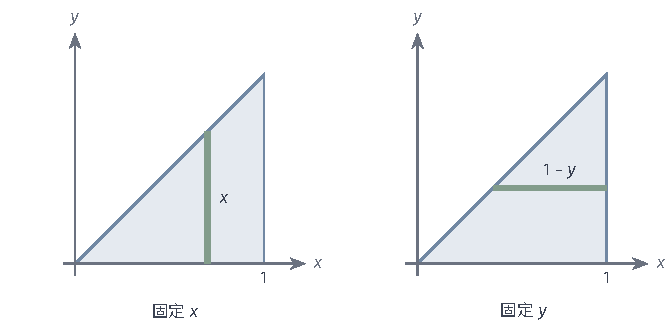
\includegraphics[width=112mm]{figures/02-vectors-matrices-and-multivariate-calculus/04-multivariate-calculus/tikz/explanation-additions/integration-slices.pdf}
\caption{区域$D=\{0\leq y\leq x\leq1\}$的两种切片。左图固定$x$，绿色线段从$y=0$到$y=x$；右图固定$y$，绿色线段从$x=y$到$x=1$。两种积分次序覆盖同一片区域。}
\label{fig:v2-integration-slices}
\end{figure}

换序还可能改变分块方式。考虑下面的三角形区域：
\[
 0\leq x\leq2,\qquad 0\leq y\leq\min(x,2-x).
\]
先对$y$积分时，上限在$x=1$处改变公式，需要分成两块。

先对$x$积分时，截面是$y\leq x\leq2-y$，$y$取遍$[0,1]$，一块即可。取$f=1$核对，两种次序都给出面积$1$。

\subsection{反常重积分与积分次序}

前面的结论只针对有界区域上的有界函数。区域无界，或被积函数在某点附近无界时，Riemann和不能直接使用。常用的做法是截断：选一族有界Jordan区域$D_\varepsilon$，它们避开奇点或截去远处，先逐个检查$f$在每个$D_\varepsilon$上Riemann可积，再考察$\int_{D_\varepsilon}f$的极限。
需要注意，沿某一族截断得到的极限，不能说明其他截断方式会给出同一结果。

例如在$(0,1]^2$上取
\[
 f(x,y)=\frac{x^2-y^2}{(x^2+y^2)^2}.
\]
对$0<\varepsilon<1$，先用矩形$D_\varepsilon=[\varepsilon,1]\times[\varepsilon^2,1]$截断。每个截断矩形都远离原点，$f$在其上连续。

先把下边界暂时放宽到$y=0$。对固定的$x>0$，$y\mapsto f(x,y)$在$[0,1]$上连续，原函数为$y/(x^2+y^2)$，所以
\[
 \int_\varepsilon^1\left(\int_0^1 f(x,y)\,\mathrm dy\right)\mathrm dx
 =\int_\varepsilon^1\frac{\mathrm dx}{1+x^2}
 \longrightarrow\frac\pi4.
\]
放宽时多算的窄条是$[\varepsilon,1]\times[0,\varepsilon^2]$。由$|x^2-y^2|\leq x^2+y^2$，窄条上
\[
 |f(x,y)|\leq\frac1{x^2+y^2}\leq\frac1{x^2},
\]
所以它的贡献不超过
\[
 \varepsilon^2\int_\varepsilon^1x^{-2}\,\mathrm dx\longrightarrow0.
\]
因此$\int_{D_\varepsilon}f\to\pi/4$。

交换两条边的截断速度，改用$E_\varepsilon=[\varepsilon^2,1]\times[\varepsilon,1]$。由$f(y,x)=-f(x,y)$，所得极限是$-\pi/4$。
两族矩形都逐渐填满同一个区域$(0,1]^2$，极限却不同，所以这里没有与截断方式无关的总量。
同样的计算也说明累次积分不能随意换序：两种次序的累次积分分别为
\[
 \int_0^1\left(\int_0^1f\,\mathrm dy\right)\mathrm dx=\frac\pi4,\qquad
 \int_0^1\left(\int_0^1f\,\mathrm dx\right)\mathrm dy=-\frac\pi4 .
\]

\section{区域积分的换元}
\label{sec:classical-change-variables}

圆盘用半径和角度描述，比用两个直角坐标简单。但换坐标不只是替换函数中的变量：参数空间中大小相同的小块，映到原空间后体积可能不同。线性映射把体积乘以其行列式的绝对值；可微映射在足够小的范围内近似线性。换元公式就是把这些局部的体积比例累计起来。

\subsection{积分换元公式}

为了保证每个点只被计算一次，并便于处理边界，先在两个开集之间取一个可微双射，再在其中选取有界的积分区域。
\begin{theorem}[经典区域积分的换元]
\label{thm:classical-change-of-variables}
设$U,V\subseteq\mathbb R^d$为开集，$T:U\to V$为$C^1$双射，逆映射也为$C^1$。设$E\subset U$为紧Jordan区域，且$T(E)$也是Jordan区域。若$f$在$T(E)$上连续，则
\begin{equation}
 \int_{T(E)}f(\bm x)\,\mathrm d\bm x
 =\int_E f(T(\bm u))|\det DT(\bm u)|\,\mathrm d\bm u.
\label{eq:classical-change-of-variables}
\end{equation}
\end{theorem}

下面说明权重$|\det DT|$的来源，并概述证明的思路。
取$E$附近的等边网格。对其中的小立方体，连续可微性给出一阶近似
\[
 T(\bm u+\bm h)-T(\bm u)=DT(\bm u)\bm h+\bm R_{\bm u}(\bm h).
\]
当$\|\bm h\|\leq\delta$时，余项满足
\[
 \|\bm R_{\bm u}(\bm h)\|\leq\eta(\delta)\|\bm h\|,
\]
其中$\eta(\delta)\to0$，而且这个界在紧集上对$\bm u$一致成立。逆映射的导数同样有界，所以小立方体的像不会在某个方向上被任意压扁。

线性部分$DT(\bm u)$把小立方体映成一个平行多面体，体积是原体积乘$|\det DT(\bm u)|$。在这个平行多面体的边界外加一层厚度与$\eta(\delta)\delta$同阶的薄层，就能夹住小立方体的真实像。薄层体积与原立方体体积之比趋于零，所以局部体积比趋于$|\det DT(\bm u)|$。

再把像区域上的Riemann和与参数区域上的加权Riemann和逐项比较。函数值替换的误差由$f$的一致连续性控制，体积替换的误差由上面一致的余项界控制，边界附近的小块由Jordan条件控制。令网格变细，就得到换元公式。
这里只给出了证明的思路。只写出某一点处的线性近似还不够，要交换整个分割和的极限，必须用到上面一致的误差控制。

定理中的全局双射条件不能省略。逆函数定理只保证每一点附近可以反解，并不保证整个区域只被覆盖一次；覆盖两次，积分就会累计两次。行列式取绝对值，消去的是定向的符号，不能消去覆盖次数。

\subsection{极坐标、柱坐标与球坐标}

平面极坐标把$(r,\theta)$映为$(r\cos\theta,r\sin\theta)$，Jacobian行列式为$r$。同样的角度宽度，在半径较大处扫过更长的弧，所以参数矩形的面积不等于平面小块的面积。面积权重为
\[
 \mathrm dA=r\,\mathrm dr\,\mathrm d\theta.
\]

\begin{figure}[!htb]
\centering
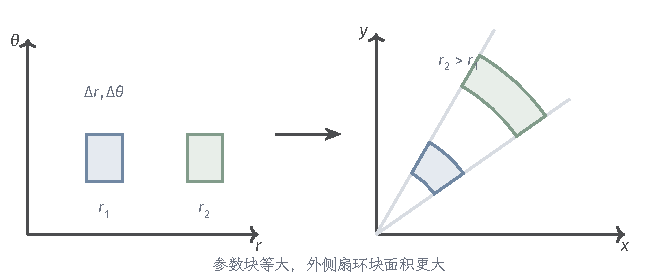
\includegraphics[width=112mm]{figures/00-shared/mathematical-preliminaries-upper/00-shared/tikz/mathematical-language-combinatorics-analysis-optimization-comprehension-additions/polar-area-weight.pdf}
\caption{径向宽度和角度宽度相同时，半径越大，对应的面积越大。小块的一阶面积为$r\Delta r\Delta\theta$，由此得到极坐标的面积权重。}
\label{fig:vol3-classical-polar-weight}
\end{figure}

极坐标在闭参数矩形上不满足换元定理的条件：原点处行列式为零，角度的两端又表示同一条射线。处理办法是先截断。限制$r\geq\varepsilon$且$\varepsilon\leq\theta\leq2\pi-\varepsilon$，在这个紧区域上应用换元定理，再令$\varepsilon\downarrow0$。
对于圆盘上的连续函数，去掉的小圆盘和窄扇形的贡献不超过函数的上界乘它们的面积，趋于零；参数一侧遗漏的部分也由有界的权重控制。

例如半径为$R$的圆盘面积为
\[
 \int_0^{2\pi}\int_0^R r\,\mathrm dr\,\mathrm d\theta=\pi R^2.
\]
若角度取到$4\pi$，圆盘内部被覆盖两次，结果也变成两倍。被积函数有奇点时，不能只说“接缝不贡献面积”而跳过截断的极限估计。

柱坐标在极坐标之外保留高度$z$，体积权重仍含因子$r$：
\[
 \mathrm dV=r\,\mathrm dr\,\mathrm d\theta\,\mathrm dz.
\]
由此，半径为$R$、高为$H$的圆柱体积为$\pi R^2H$。轴线和角度接缝的处理与极坐标相同。

球坐标使用到原点的距离$\rho$、从正$z$轴量起的极角$\varphi$和方位角$\theta$：
\[
 T(\rho,\varphi,\theta)
 =(\rho\sin\varphi\cos\theta,\rho\sin\varphi\sin\theta,\rho\cos\varphi).
\]
三个参数各自变化时，点沿三个相互正交的方向移动，长度的放大比例分别是$1$、$\rho$和$\rho\sin\varphi$。三者相乘就是体积权重，直接计算Jacobian行列式也得到同一结果：
\[
 \mathrm dV=\rho^2\sin\varphi\,\mathrm d\rho\,\mathrm d\varphi\,\mathrm d\theta.
\]

在$\rho>0$、$0<\varphi<\pi$和一个长度为$2\pi$的开角度区间上，这个映射是双射，像是空间去掉$z$轴和一个接缝半平面后的部分。计算球内连续函数的积分时，先截去原点、极轴和接缝附近的小区域，再用函数的有界性估计遗漏的部分。由此得到球的体积
\[
 \int_0^{2\pi}\int_0^\pi\int_0^R
 \rho^2\sin\varphi\,\mathrm d\rho\,\mathrm d\varphi\,\mathrm d\theta
 =\frac{4\pi R^3}{3}.
\]

\subsection{线性换元}

线性换元可以把斜着放的区域变成坐标盒。
设$D$由$0\leq x+y\leq2$和$0\leq x-y\leq2$围成，求$\int_D(x+y)\,\mathrm d(x,y)$。令$u=x+y$、$v=x-y$，参数区域就是$[0,2]^2$，逆变换为
\[
 x=\frac{u+v}2,\qquad y=\frac{u-v}2.
\]
逆变换的Jacobian行列式为$-1/2$，所以面积权重为$1/2$。于是
\[
 \int_D(x+y)\,\mathrm d(x,y)
 =\int_0^2\int_0^2\frac u2\,\mathrm du\,\mathrm dv=2.
\]

这个结果可以用另外两个量核对。取被积函数为$1$，同样的换元给出区域面积$2$。$x+y=u$在区域上的平均值为$1$，平均值乘面积也是$2$。区域、权重和积分值由此得到同时检验。

\section{参数积分}

若被积函数还依赖一个参数，积分值就随参数变化，成为参数的函数。例如一块薄板的密度随时间改变，总质量就是时间的函数。
判断这个函数是否连续、能否求导，需要控制整个积分区域上的变化；只在每一点处成立的极限不够。本节固定紧Jordan区域$D$，用连续性提供这种统一的控制。

\subsection{参数积分的连续性}

设$K$为紧参数区域，$f$在$D\times K$上连续，记
\[
 F(\bm t)=\int_D f(\bm x,\bm t)\,\mathrm d\bm x.
\]
$D\times K$是紧集，$f$在其上一致连续，所以$\bm t\to\bm s$时，
\[
 \sup_{\bm x\in D}|f(\bm x,\bm t)-f(\bm x,\bm s)|\longrightarrow0.
\]
用绝对值估计，
\[
 |F(\bm t)-F(\bm s)|
 \leq |D|\sup_{\bm x\in D}|f(\bm x,\bm t)-f(\bm x,\bm s)|\longrightarrow0,
\]
所以$F$连续。
参数区域不必整体有界。讨论某个内点附近的连续性时，取包含该点的一个小闭盒作为$K$即可。

\subsection{积分号下求导}

求导的思路相同：把参数差商的极限放进积分号内，关键是证明差商对所有$\bm x\in D$一致收敛。

设参数取自开集，$f$和各参数偏导数$\partial_{t_j}f$在$D$与参数邻域的乘积上连续。固定一个参数点，取它的一个足够小的闭邻域。由一元中值定理，沿$t_j$方向的差商等于附近某个参数处的偏导数值。偏导数在紧集上一致连续，所以差商对全部$\bm x\in D$一致趋于$\partial_{t_j}f$。对差商与偏导数之差积分，并用上一小节的上确界估计，得到
\begin{equation}
 \partial_{t_j}F(\bm t)=\int_D\partial_{t_j}f(\bm x,\bm t)\,\mathrm d\bm x.
\label{eq:classical-differentiate-under-integral}
\end{equation}

右侧又是一个被积函数连续的参数积分，由上一小节，它是参数的连续函数。于是$F$的各个偏导数都存在且连续，由连续偏导数判据，$F$是$C^1$函数，全微分为
\[
 DF_{\bm t}[\bm h]=\int_D D_{\bm t}f(\bm x,\bm t)[\bm h]\,\mathrm d\bm x.
\]
整体可微是由连续偏导数推出的；只验证每个方向上的极限，还不能得到这一结论。

例如$F(t)=\int_0^1 e^{tx}\,\mathrm dx$在任意有界参数区间上都满足上述条件，所以
\[
 F'(0)=\int_0^1x\,\mathrm dx=\frac12.
\]
显式表达式$F(t)=(e^t-1)/t$在$t=0$处有可去奇点；在积分号下求导，就不必处理它。

\subsection{变限参数积分}

积分区间也随参数变化时，积分值的变化来自两部分：区间内部的被积函数在变，两端又新添或移除了细条。

设$a(t),b(t)$为$C^1$函数，$f(x,t)$及$\partial_tf(x,t)$在所需区间附近连续。把积分写成从某个固定点到$b(t)$的积分减去从该点到$a(t)$的积分，对上限用一元基本定理，对被积函数中的参数用式~\eqref{eq:classical-differentiate-under-integral}，再由链式法则合并，得到
\begin{equation}
 \frac{\mathrm d}{\mathrm dt}\int_{a(t)}^{b(t)}f(x,t)\,\mathrm dx
 =\int_{a(t)}^{b(t)}\partial_tf(x,t)\,\mathrm dx
 +f(b(t),t)b'(t)-f(a(t),t)a'(t).
\label{eq:classical-variable-limit-derivative}
\end{equation}
第一项来自被积函数的变化，后两项来自端点的移动。上端向右移动会增加积分，下端向右移动会减少积分，所以两个边界项符号相反。

有多个参数时，对每个参数分别求偏导；也可以把$a'$、$b'$和$\partial_tf$换成作用于同一参数增量的全微分。更一般的移动区域会产生沿整个边界的贡献，本章只在上述区间变限的情形使用这一规则。

\FloatBarrier
\section{本章小结}
\label{sec:region-integrals-summary}

区域积分把密度累计成总量。Jordan区域是能用有限个坐标盒从内外两侧任意逼近的有界集合，等价地，它的边界能被总体积任意小的有限个盒覆盖。边界因而不影响有界函数的累计：在区域闭包上连续的函数可积，分块连续的有界函数也可积；有界本身则不够，例如有理点的指示函数不可积。积分继承有限和的线性、保序、绝对值估计与区域可加性，体积、质量、平均值和质心都是区域积分。

累次积分把一次多维累计化为几次一元积分。被积函数连续、区域由连续的边界函数描述时，按截面分组的Riemann和收敛到累次积分，两种次序给出同一个值；换序时要重新求出区域在另一坐标轴上的投影和截面，必要时改变分块。区域无界或被积函数无界时，有界情形的结论不能直接使用：要先截断再取极限，而不同的截断方式和不同的积分次序可以给出不同的结果。

换元时，可微映射在一点附近近似线性，Jacobian行列式的绝对值给出局部体积的缩放，换元公式把这些倍数累计起来。公式要求两个开集之间的$C^1$双射及$C^1$逆，绝对值消去的是定向的符号，消不去覆盖次数。极坐标、柱坐标和球坐标的权重分别为$r$、$r$与$\rho^2\sin\varphi$；它们在原点、轴线和角度接缝处不满足条件，须先截去这些部分，再用被积函数的有界性控制遗漏的贡献。

参数积分在紧Jordan区域上依赖统一控制：被积函数在区域与参数集的乘积上连续时，积分随参数连续；参数偏导数也联合连续时，可以在积分号下求导，并由连续偏导数推出全微分。只有逐点的极限不够。积分限随参数移动时，导数除了积分号下的项，还要加上两端新增或移除的细条贡献。下一章把累计的范围从区域换成曲线。


\par\Needspace{10\baselineskip}
\chapter{路径积分}
\label{sec:multivariable-path-integration}
\label{chap:path-integrals}

区域积分累计铺满一块区域的量。许多问题却只沿一条曲线累计。一根弯曲细铁丝的质量，由各处的线密度和铁丝的长度决定。把物体沿一条路线推过去，推力做的功不仅取决于力的大小和路线的长度，还取决于力与前进方向的夹角。

两类问题都沿曲线累计，被积对象却不同：线密度在每一点给出一个数，是标量场；力在每一点给出一个带方向的量，是向量场（第~\ref{sec:multivariable-functions-and-fields}节）。本章要回答：怎样沿曲线按长度累计一个标量场，怎样沿行进方向累计一个向量场的作用，以及后一种累计什么时候只取决于起点和终点。

相应地有两种路径积分。第一类路径积分把曲线切成小段，用每段上的函数值乘这段的长度再相加，铁丝的质量就这样算出，它与沿哪个方向走过曲线无关。
第二类路径积分在每一小段上取力与这段有向位移的内积，只保留力沿前进方向的分量，再把这些数相加。反向行走时每段位移都反号，积分也随之变号。

第一节用参数路径描述一次行进，区分曲线的像、参数的快慢、行进方向与重复覆盖，并用速度长度的积分计算弧长。第二节在此基础上按弧长累计标量场；第三节改为累计向量场的切向分量，方向随之进入结果。第四节研究功只依赖端点的情形，这对应物理中保守力与势能的关系：势函数把沿途累计化为端点差，交叉偏导相等给出可以检查的微分条件，而定义域中的洞会使这一条件失效。

本章的参数积分都是一元Riemann积分；路径无关的判别要用到第~\ref{chap:multivariate-differentiation}章的链式法则、混合偏导数的交换，以及第~\ref{chap:region-integrals}章的积分号下求导。经典构造可参考\scite{math-openstax-calculus3}。

\section{参数路径与弧长}
\label{sec:multivariable-line-integrals}

描述一次行进，需要知道每个时刻所在的位置。位置随时间连续变化，就得到一条路径；位置对时间的导数是速度，速度的大小称为速率。速率恒定时，速率乘经过的时间就是走过的路程；速率随时间变化时，路程是速率对时间的积分。

\subsection{路径的定义}

\paragraph{参数化路径}

不妨把参数$t$看成时间，把$\gamma(t)$看成一个质点在时刻$t$所在的位置。经过同一组位置时，可以走得快或慢，可以从任一端出发，也可以来回走好几遍。只记下经过了哪些点，就会丢失这些信息。用区间到空间的连续映射描述行进，位置和先后次序就一起保留下来。
\begin{definition}[路径]
设$a<b$。连续映射$\gamma:[a,b]\to\mathbb R^d$称为一条\term{路径}（path），$\gamma(a)$和$\gamma(b)$分别为起点和终点；若两者相等，称为闭路径。
集合$C=\gamma([a,b])$称为路径的像。
\end{definition}

像集$C$只记录质点经过的位置，参数$t$还规定了经过的先后次序，所以同一个像集可以对应行进方式完全不同的路径。
\begin{example}[同一条对角线段上的三条路径]
\label{ex:analysis-diagonal-segment-paths}
以下三条平面路径的像都是连接$(0,0)$与$(1,1)$的对角线段：
\begin{itemize}
 \item $\gamma(t)=(t,t)^\top$，$0\leq t\leq1$，从$(0,0)$走到$(1,1)$，速度为$(1,1)^\top$；
 \item $\eta(u)=(u/2,u/2)^\top$，$0\leq u\leq2$，同样从$(0,0)$走到$(1,1)$，速度减半为$(1/2,1/2)^\top$，用时加倍；
 \item $\rho(t)=(t,t)^\top$（$0\leq t\leq1$）、$\rho(t)=(2-t,2-t)^\top$（$1\leq t\leq2$），先走到$(1,1)$再原路返回。
\end{itemize}
$\gamma$与$\eta$只是快慢不同，线段上每个点都恰好经过一次。$\rho$的像仍是这条线段，但每个内点被经过两次：去程一次，回程一次。
\end{example}

后面会看到，两种路径积分对$\gamma$与$\eta$给出相同的结果。沿$\rho$按长度累计时，结果是沿$\gamma$的两倍；按有向位移累计时，去程与回程恰好抵消。
所以路径积分是沿一次行进定义的，只知道像集还不能确定它。计算一根铁丝的质量时，应选一条把铁丝恰好走一遍的路径。

\paragraph{分段光滑路径}

示例~\ref{ex:analysis-diagonal-segment-paths}中的往返路径$\rho$在$t=1$处突然掉头，正方形的边界在四个角处突然转向。这些位置没有唯一的切线方向，但在每一段直线上，速度都存在且连续。为了把折线、多边形边界这类常见路径纳入计算，允许路径在有限个参数点处分段。
\begin{definition}[分段光滑路径]
若存在分割$a=t_0<t_1<\cdots<t_n=b$，使$\gamma$在每个$[t_{j-1},t_j]$上为$C^1$映射，称$\gamma$为分段$C^1$路径，也称分段光滑路径。
若每段内部还满足$\gamma'(t)\neq\bm0$，称该路径分段正则。
\end{definition}

这里“在闭区间$[t_{j-1},t_j]$上为$C^1$”是指该段内部的导数连续，并能连续延拓到该段的两个端点；相邻两段在公共端点处的导数不必相同。
例如$\rho$在$[0,1]$上的速度为$(1,1)^\top$，在$[1,2]$上的速度为$(-1,-1)^\top$。两段在$t=1$处的速度不同，但各自连续，所以$\rho$是分段$C^1$路径。

本章的路径积分都在分段$C^1$路径上定义。折点只有有限个，改变有界函数在有限个点上的取值不影响Riemann积分，所以折点处的速度怎样取值都不影响参数积分。
分段正则要求每段内部速度不为零，排除了质点中途停住的情形。本章的积分不要求路径正则；后面用到单位切向量时，只在速度非零处使用它。

\subsection{路径的长度}

\paragraph{弧长}

测量一条弯曲道路的长度时，可以在路上依次插几根标杆，量出相邻标杆之间的直线距离再相加。每段直线距离都不超过对应那段路的实际长度，所以折线长度不会超过道路长度。在两根标杆之间再插一根，由三角不等式，新折线不会变短。标杆越密，折线越贴近道路，因此把道路的长度定义为所有内接折线长度的上确界。
\begin{definition}[路径的弧长]
路径$\gamma:[a,b]\to\mathbb R^d$的弧长定义为
\[
 \ell(\gamma)=\sup_{a=t_0<\cdots<t_n=b}
 \sum_{j=1}^n\lVert\gamma(t_j)-\gamma(t_{j-1})\rVert_2.
\]
上确界取遍$[a,b]$的全部有限分割；若此值有限，称路径可求长。
\end{definition}

这个定义只用到路径上点的位置，不需要导数，所以任何连续路径都可以讨论它是否可求长。

对分段光滑路径，弧长可以用速度直接计算。在一小段参数区间$[t_{j-1},t_j]$上，质点的位移近似为速度乘时间：
\[
 \gamma(t_j)-\gamma(t_{j-1})\approx\gamma'(t_{j-1})(t_j-t_{j-1}).
\]
所以这一小段的长度近似为速率$\lVert\gamma'(t_{j-1})\rVert_2$乘时间，汽车里程表就是这样累计路程的。把这些乘积相加，再令分割变细，就得到下面的公式。
\begin{theorem}[分段光滑路径的弧长]
若$\gamma:[a,b]\to\mathbb R^d$分段$C^1$，则它可求长，且
\[
 \ell(\gamma)=\int_a^b\lVert\gamma'(t)\rVert_2\,\mathrm dt.
\]
\end{theorem}
\begin{proof}
加入分点不会使折线变短，所以计算上确界时只需考虑包含全部折点的分割；这样的折线长度按光滑段相加，弧长也按段相加。因此只需在一段$C^1$区间上证明，再把各段的等式相加。证明分两步：先说明任何折线都不比速度积分长，再说明足够细的折线与速度积分相差任意小。

第一步。对该段中的$\alpha<\beta$，由各坐标分量的一元基本定理，
$\gamma(\beta)-\gamma(\alpha)=\int_\alpha^\beta\gamma'(t)\,\mathrm dt$，这里向量的积分表示对各分量分别积分。
若弦$\gamma(\beta)-\gamma(\alpha)$非零，取它方向上的单位向量$\bm u$，则由Cauchy--Schwarz不等式
\[
 \lVert\gamma(\beta)-\gamma(\alpha)\rVert_2
 =\bm u^\top\bigl(\gamma(\beta)-\gamma(\alpha)\bigr)
 =\int_\alpha^\beta\bm u^\top\gamma'(t)\,\mathrm dt
 \leq\int_\alpha^\beta\lVert\gamma'(t)\rVert_2\,\mathrm dt;
\]
弦为零时这个不等式直接成立。同样的推理说明，任何连续向量值函数$\bm v$都满足$\lVert\int_\alpha^\beta\bm v\,\mathrm dt\rVert_2\leq\int_\alpha^\beta\lVert\bm v\rVert_2\,\mathrm dt$。
对任意分割把各段弦长相加，可知任意内接折线的长度都不超过$\int_a^b\lVert\gamma'\rVert_2\,\mathrm dt$，所以上确界也不超过它。

第二步。$\gamma'$在紧区间上一致连续。给定$\varepsilon>0$，取足够细的分割，使每个小区间上任意两点的$\gamma'$相距小于$\varepsilon$，并记$\Delta t_j=t_j-t_{j-1}$。
在第$j$个小区间上，
\[
 \gamma(t_j)-\gamma(t_{j-1})-\gamma'(t_{j-1})\Delta t_j
 =\int_{t_{j-1}}^{t_j}\bigl(\gamma'(t)-\gamma'(t_{j-1})\bigr)\,\mathrm dt,
\]
由第一步的范数不等式，它的范数不超过$\varepsilon\Delta t_j$；于是这一段的弦长与$\lVert\gamma'(t_{j-1})\rVert_2\Delta t_j$之差不超过$\varepsilon\Delta t_j$。
同一小区间上，$\int\lVert\gamma'\rVert_2\,\mathrm dt$与$\lVert\gamma'(t_{j-1})\rVert_2\Delta t_j$的差也不超过$\varepsilon\Delta t_j$。
两项相加后对$j$求和，速度积分与这条折线长度的差不超过$2\varepsilon(b-a)$，所以上确界不小于速度积分减$2\varepsilon(b-a)$。令$\varepsilon\downarrow0$，得到反向不等式。
\end{proof}

用这个公式可以计算示例~\ref{ex:analysis-diagonal-segment-paths}中三条路径的长度，并检验圆周长公式。
\begin{example}[对角线段与圆周的弧长]
对角线段$\gamma(t)=(t,t)^\top$，$0\leq t\leq1$，速度为$(1,1)^\top$，速率为$\sqrt2$，所以$\ell(\gamma)=\int_0^1\sqrt2\,\mathrm dt=\sqrt2$。两个坐标各变化$1$，走过的距离却不是$1+1=2$，而是斜边的长度。

慢速路径$\eta$的速率为$\sqrt2/2$，用时为$2$，长度为$\int_0^2(\sqrt2/2)\,\mathrm du=\sqrt2$。往返路径$\rho$在两段上的速率都是$\sqrt2$，总用时为$2$，长度为$2\sqrt2$。

半径为$r$的圆周可以参数化为$t\mapsto(r\cos t,r\sin t)^\top$，$0\leq t\leq2\pi$。速度为$(-r\sin t,r\cos t)^\top$，速率恒为$r$，长度为$\int_0^{2\pi}r\,\mathrm dt=2\pi r$，与圆周长公式一致。
\end{example}

$\gamma$与$\eta$的长度相同，因为速率减半恰好被用时加倍抵消；$\rho$的长度是$\gamma$的两倍，因为弧长把经过的次数也计算在内。

记$s(t)=\int_a^t\lVert\gamma'(u)\rVert_2\,\mathrm du$为截至时刻$t$累计走过的路程，它就是里程表在时刻$t$的读数。在每个光滑段内部，$s$对$t$的导数是速率$\lVert\gamma'(t)\rVert_2$，因此常把长度权重简写为
$\mathrm ds=\lVert\gamma'(t)\rVert_2\,\mathrm dt$，读作“一小段时间$\mathrm dt$内走过的一小段路程”。

\section{第一类路径积分}

第一类路径积分的被积对象是定义在曲线上的标量函数，例如铁丝各处的线密度或一条道路沿线各处的温度。每一小段的贡献是函数值乘这一小段的实际长度，因此它只需要路程这一个权重，不涉及方向。

\subsection{定义与可积性}

\paragraph{按弧长的积分}

设一根铁丝沿路径$\gamma$放置，$h(\bm x)$是它在点$\bm x$处的线密度，即单位长度的质量。线密度为常数时，质量等于密度乘长度；密度随位置变化时，把铁丝切成许多小段，每段上的密度近似为常数。
在参数小区间$[t_{j-1},t_j]$对应的一段上取一个时刻$\xi_j$，这段的质量约为
\[
 h(\gamma(\xi_j))\,\lVert\gamma'(\xi_j)\rVert_2\,(t_j-t_{j-1}),
\]
即“该处密度”乘“该段长度”。把各段相加，就得到参数区间上函数$h(\gamma(t))\lVert\gamma'(t)\rVert_2$的积分和，所以用这个函数的一元积分定义沿路径的累计。这里先讨论沿路径连续的密度；有限分段连续的密度可逐段处理。
\begin{definition}[第一类路径积分]
设$\gamma:[a,b]\to\mathbb R^d$分段$C^1$，$h$在路径像集上连续。定义\term{第一类路径积分}为
\begin{equation}
 \int_\gamma h\,\mathrm ds=\int_a^b h(\gamma(t))\|\gamma'(t)\|_2\,\mathrm dt.
 \label{eq:analysis-scalar-line-integral}
\end{equation}
右侧按各光滑段的一元Riemann积分相加，因被积函数分段连续而存在。
\end{definition}

取$h=1$，积分就是弧长$\ell(\gamma)$；$h$是非负线密度时，积分是铁丝的总质量。

若$\ell(\gamma)>0$，比值
\[
 \bar h=\frac1{\ell(\gamma)}\int_\gamma h\,\mathrm ds
\]
是$h$沿曲线按长度的平均值：沿一条道路每隔相同路程记录一次温度再求平均，记录越密，结果越接近$\bar h$。
这里的平均按路程加权，而不按参数时间加权。若一辆车在某段路上开得很慢，按时间平均会让这段路的温度占更大比重，按路程平均则不受车速影响。

用一根密度不均匀的半圆铁丝可以说明质量和平均线密度的计算。
\begin{example}[上半圆铁丝的质量与平均线密度]
\label{ex:analysis-semicircle-wire}
沿上半单位圆$\gamma(t)=(\cos t,\sin t)^\top$，$0\leq t\leq\pi$，放一根铁丝，线密度为$h(x,y)=y$，即越高的地方越重。速度为$(-\sin t,\cos t)^\top$，速率恒为$1$，所以总质量为
\[
 \int_\gamma y\,\mathrm ds=\int_0^\pi\sin t\,\mathrm dt=2.
\]
铁丝长度为$\pi$，平均线密度为$\bar h=2/\pi\approx0.64$。两端$(\pm1,0)$处密度为零，顶点$(0,1)$处密度为$1$，平均值落在两者之间。
\end{example}
这条参数化的速率恒为$1$，参数时间与路程同步增长，所以按时间平均也得到$2/\pi$；速率不恒定时，两种平均一般不同。

\subsection{积分的基本性质}

下面的函数都假设在所讨论路径的像集上连续，或沿各光滑段分段连续，从而相应积分存在。把定义式~\eqref{eq:analysis-scalar-line-integral}代入一元Riemann积分的相应性质，就逐项得到这些结论。用铁丝质量来读，每条性质都有直接的含义。

\paragraph{线性}

对函数$h,k$和实数$c$，有
\[
 \int_\gamma(h+k)\,\mathrm ds=\int_\gamma h\,\mathrm ds+\int_\gamma k\,\mathrm ds,
 \qquad
 \int_\gamma ch\,\mathrm ds=c\int_\gamma h\,\mathrm ds.
\]
两式都来自一元积分的线性；取$c=-1$再用第一式，就得到差的积分等于积分之差。若铁丝由两种材料叠合而成，总质量等于两种材料各自的质量之和；把每一小段的密度同时放大$c$倍，总质量也放大$c$倍。

\paragraph{路径拼接}

若$\gamma_1$的终点是$\gamma_2$的起点，记先走$\gamma_1$、再走$\gamma_2$的拼接路径为$\gamma_1*\gamma_2$，则
\[
 \int_{\gamma_1*\gamma_2}h\,\mathrm ds
 =\int_{\gamma_1}h\,\mathrm ds+\int_{\gamma_2}h\,\mathrm ds.
\]
拼接路径的参数区间由两段参数区间首尾相接而成，等式来自一元积分对区间的可加性。逐段计算折线和多边形边界上的积分，依据的就是这个等式。

两段路径有重叠部分时，重叠部分的贡献会计入两次。示例~\ref{ex:analysis-diagonal-segment-paths}中的往返路径$\rho$由去程$\gamma$与原路返回的一段拼成；返回段$(2-t,2-t)^\top$，$1\leq t\leq2$，经换元$u=2-t$化为$\gamma$上的同一个积分，所以沿$\rho$的积分是沿$\gamma$的两倍。

\paragraph{重参数化与方向无关}

同一根铁丝，无论从哪一端开始称量、量得快还是慢，质量都不变。改变快慢和方向，都可以用换参数表示。设$t=\sigma(u)$是两个参数区间之间单调、端点相配的分段$C^1$微分同胚，新路径$\gamma\circ\sigma$在时刻$u$位于$\gamma(\sigma(u))$。
链式法则给出新速度$(\gamma\circ\sigma)'(u)=\gamma'(\sigma(u))\sigma'(u)$，所以新速率为
$\lVert\gamma'(\sigma(u))\rVert_2|\sigma'(u)|$。代入定义并用一元换元公式$t=\sigma(u)$，得到
\[
 \int_{\gamma\circ\sigma}h\,\mathrm ds=\int_\gamma h\,\mathrm ds.
\]

走得慢时速率变小，但用时按同一比例变长，乘积不变。$\sigma$递减时路径反向，绝对值$|\sigma'|$仍给出非负的长度权重，所以反向行进也不改变第一类积分。
在示例~\ref{ex:analysis-diagonal-segment-paths}中，$\eta=\gamma\circ\sigma$，其中$\sigma(u)=u/2$，$0\leq u\leq2$，所以沿$\eta$与沿$\gamma$的第一类积分相同，弧长都是$\sqrt2$。换参数只改变快慢和方向，不改变经过的次数，所以往返路径$\rho$不是$\gamma$的重参数化。

\paragraph{单调性}

若在路径上处处有$h\leq k$，则
\[
 \int_\gamma h\,\mathrm ds\leq\int_\gamma k\,\mathrm ds.
\]
这是因为长度权重$\lVert\gamma'\rVert_2$非负，被积函数的大小关系乘以权重后保持不变。密度处处较小的铁丝，总质量也较小。

\paragraph{绝对值不等式}

由一元积分的绝对值不等式可得
\[
 \left|\int_\gamma h\,\mathrm ds\right|
 \leq\int_\gamma|h|\,\mathrm ds
 \leq\sup_C|h|\,\ell(\gamma).
\]
连续函数在紧的像集$C$上有界，所以最后一项有限：累计量的绝对值不超过函数绝对值的上确界乘路径长度。例如在示例~\ref{ex:analysis-semicircle-wire}中，密度$y$不超过$1$，质量$2$确实不超过$1\cdot\pi$。

\subsection{积分的计算}

计算第一类路径积分分三步：给曲线选一条把它恰好走一遍的参数化；把$h(\gamma(t))$乘速率$\lVert\gamma'(t)\rVert_2$；在参数区间上做一元积分，有折点时在折点两侧分别计算再相加。
先在示例~\ref{ex:analysis-diagonal-segment-paths}的对角线段上积分一个线性函数。
\begin{example}[沿对角线段积分$x+y$]
取$\gamma(t)=(t,t)^\top$，$0\leq t\leq1$，$h(x,y)=x+y$。沿路径有$h(\gamma(t))=2t$，速率为$\sqrt2$，所以
\[
 \int_\gamma h\,\mathrm ds=\int_0^1 2t\cdot\sqrt2\,\mathrm dt=\sqrt2.
\]
线段长为$\sqrt2$，平均值为$\sqrt2/\sqrt2=1$，恰是$h$在线段中点$(1/2,1/2)$的值，因为$h$沿这条线段随路程线性变化。
\end{example}
若漏掉速率而只计算$\int_0^12t\,\mathrm dt=1$，得到的是按参数时间的累计，比按长度的累计少了速率因子$\sqrt2$。第一类路径积分也不是线段下方某块平面区域的面积：区域积分按面积加权，这里的权重是沿线段的长度。

许多平面曲线写成函数图像$y=\psi(x)$。设$\psi$在$[a,b]$上为$C^1$，取沿$x$递增的图像路径$\gamma(x)=(x,\psi(x))^\top$，$a\leq x\leq b$。它以$x$本身作参数，速度为$(1,\psi'(x))^\top$，于是
\[
 \int_\gamma h\,\mathrm ds
 =\int_a^b h(x,\psi(x))\sqrt{1+\psi'(x)^2}\,\mathrm dx.
\]
根号是图像路径的速率：自变量前进$\mathrm dx$时，曲线同时升高约$\psi'(x)\,\mathrm dx$，斜边长约为$\sqrt{1+\psi'(x)^2}\,\mathrm dx$。曲线越陡，同一个$\mathrm dx$对应的路程越长，因此不能只写$\mathrm dx$。

用这个公式可以计算一段抛物线铁丝的质量。
\begin{example}[抛物线铁丝的质量]
沿抛物线段$y=x^2$，$0\leq x\leq1$，放一根铁丝，线密度为$h(x,y)=x$。这里$\psi(x)=x^2$，$\psi'(x)=2x$，速率为$\sqrt{1+4x^2}$。令$w=1+4x^2$，则$\mathrm dw=8x\,\mathrm dx$，$w$从$1$变到$5$，所以
\[
 \int_\gamma x\,\mathrm ds=\int_0^1x\sqrt{1+4x^2}\,\mathrm dx
 =\frac18\int_1^5\sqrt w\,\mathrm dw=\frac{5\sqrt5-1}{12}\approx0.85.
\]
\end{example}
若漏写根号，只会得到$\int_0^1x\,\mathrm dx=1/2$，丢掉了曲线变陡后多出的长度。

\section{第二类路径积分}

第一类积分只问每段有多长，做功问题还要问这段朝哪个方向走。推一辆车时，力与前进方向一致才完全用于推动；力与前进方向垂直时不做功；力与前进方向相反时做负功。描述这种累计之前，先要说清“每一点有一个力”是什么意思。

\subsection{定义与可积性}

\paragraph{向量场}

力可以随位置变化：地面附近的重力处处竖直向下，太阳对行星的引力指向太阳，并随距离减弱。河水在每一点有一个流速，流速同样有大小和方向。按定义~\ref{def:multivariable-vector-field}，这类对象是向量场$\bm F:U\subseteq\mathbb R^d\to\mathbb R^d$：输入是位置，输出是放在该位置的一个向量，常画成从该点出发的箭头。输出与位置同维，才能与路径的速度向量作内积。

下面是本章反复使用的三个平面例子：
\begin{itemize}
 \item 常向量场$\bm F(x,y)=(0,-mg)^\top$描述地面附近质量为$m$的物体所受重力，其中$g$是重力加速度，箭头处处竖直向下、长度相同；
 \item $\bm F(x,y)=(x,y)^\top$的箭头从原点向外，离原点越远越长；
 \item $\bm F(x,y)=(-y,x)^\top$的箭头与以原点为圆心的圆相切，按逆时针方向，长度等于到原点的距离。它是绕原点以角速度$1$旋转的圆盘上各点的速度，本部分称它为旋转场。
\end{itemize}
旋转场与位置向量处处垂直，因为$(-y)\cdot x+x\cdot y=0$。

\paragraph{有向线积分}

先看最简单的情形：常力$\bm F$使物体沿直线产生位移$\Delta\bm r$。中学物理中的功是$\lVert\bm F\rVert_2\lVert\Delta\bm r\rVert_2\cos\theta$，其中$\theta$是力与位移的夹角，这正是内积$\bm F^\top\Delta\bm r$。把力分解为沿位移方向和垂直于位移方向的两部分，只有前一部分做功：$\theta<\pi/2$时功为正，$\theta=\pi/2$时为零，$\theta>\pi/2$时为负。

路线弯曲、力随位置变化时，把路径切成许多小段。参数小区间$[t_{j-1},t_j]$上的位移近似为$\gamma'(\xi_j)(t_j-t_{j-1})$，力近似为常力$\bm F(\gamma(\xi_j))$，这段的功约为
\[
 \bm F(\gamma(\xi_j))^\top\gamma'(\xi_j)\,(t_j-t_{j-1}).
\]
各段相加就是参数区间上函数$\bm F(\gamma(t))^\top\gamma'(t)$的积分和。这里乘的是速度向量本身，不是速率，所以位移的方向保留在被积函数中。
\begin{definition}[第二类路径积分]
设$\gamma:[a,b]\to U$分段$C^1$，$\bm F:U\to\mathbb R^d$为向量场。
若$\bm F$在路径像集上连续，定义\term{第二类路径积分}（vector line integral）为
\begin{equation}
 \int_\gamma\bm F\mathbin{\cdot}\mathrm d\bm r
 =\int_a^b\bm F(\gamma(t))^\top\gamma'(t)\,\mathrm dt.
 \label{eq:analysis-vector-line-integral}
\end{equation}
\end{definition}

记号$\mathrm d\bm r$表示一小段有向位移$\gamma'(t)\,\mathrm dt$，$\bm F\cdot\mathrm d\bm r$是这一小段上的功。
在平面中，若$\bm F=(P,Q)^\top$，路径为$\gamma(t)=(x(t),y(t))^\top$，则被积函数是$P\,x'(t)+Q\,y'(t)$，因此积分也写成$\int_\gamma P\,\mathrm dx+Q\,\mathrm dy$：$P\,\mathrm dx$是力的水平分量在水平位移上做的功，$Q\,\mathrm dy$是竖直分量在竖直位移上做的功。三维中再加上第三个分量$R$对应的$R\,\mathrm dz$。

$\bm F$在路径像集上连续时，复合函数$\bm F\circ\gamma$在各光滑段上连续，被积函数在各段上连续，所以参数积分存在。

两类路径积分可以用单位切向量联系起来。在速度非零处，单位切向量$\bm\tau=\gamma'/\lVert\gamma'\rVert_2$指向前进方向，于是
\[
 \bm F^\top\gamma'\,\mathrm dt=(\bm F^\top\bm\tau)\,\lVert\gamma'\rVert_2\,\mathrm dt=(\bm F^\top\bm\tau)\,\mathrm ds.
\]
$\bm F^\top\bm\tau$是力在前进方向上的分量，称为切向分量。速度为零处，左侧的被积函数为零，右侧的长度权重$\lVert\gamma'\rVert_2$也为零，不必定义$\bm\tau$。所以第二类积分等于切向分量的第一类积分：功是沿前进方向的力乘走过的路程，再累计起来。
两者的区别在于，切向分量依赖行进方向。反向行走时$\bm\tau$变为$-\bm\tau$，切向分量变号，积分也变号；第一类积分的被积函数则与方向无关。

若$\bm F$是流体的速度场，沿闭路径的积分累计的是流速沿这条闭路径的切向分量，称为\term{环流}（circulation）。环流为正，表示流体总体上倾向于沿所选方向绕这条闭路径流动。
例如沿单位圆逆时针行进时，旋转场$(-y,x)^\top$的切向分量处处为$1$，一周的环流是$1\times2\pi=2\pi$。

图~\ref{fig:analysis-process-line-density-work}用同一条线段对照两类积分：左图按长度累计常数密度，右图只累计位移的水平分量。
\begin{figure}[!htbp]
 \centering
 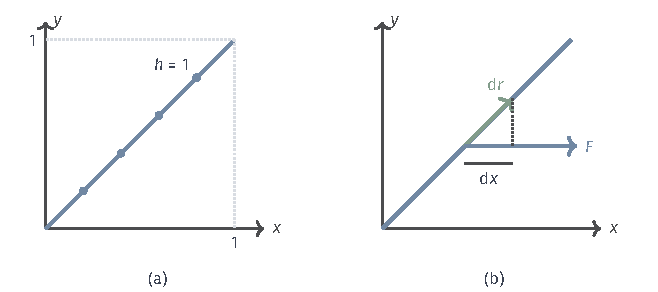
\includegraphics[width=112mm]{figures/00-shared/mathematical-preliminaries-upper/00-shared/tikz/chapter3-concept-processes/line-density-work.pdf}
 \caption{路径均为$\gamma(t)=(t,t)^\top$，$0\leq t\leq1$。(a) 常数线密度$h=1$按弧长累计，得到$\sqrt2$。(b) 常向量场$\bm F=(1,0)^\top$只取位移的水平分量，做功为$1$；图中$\mathrm dx$是$\mathrm d\bm r$的水平投影。相同路径、不同被积对象和权重给出不同积分。}
 \label{fig:analysis-process-line-density-work}
\end{figure}

\subsection{积分的基本性质}

以下向量场都假设在路径像集上连续。这些性质由内积的线性和一元Riemann积分的相应性质得到。线性说明功对力是线性的；拼接、方向反转和重参数化说明功怎样随路径变化；最后的不等式估计功的大小。

\paragraph{线性}

对向量场$\bm F,\bm G$和实数$c$，有
\[
 \int_\gamma(\bm F+\bm G)\cdot\mathrm d\bm r
 =\int_\gamma\bm F\cdot\mathrm d\bm r+\int_\gamma\bm G\cdot\mathrm d\bm r,
 \qquad
 \int_\gamma c\bm F\cdot\mathrm d\bm r
 =c\int_\gamma\bm F\cdot\mathrm d\bm r.
\]
两个力同时作用时，合力做的功等于两个力各自做功之和。力放大$c$倍，功也放大$c$倍；$c<0$时力反向，功变号。两式结合，就得到差的积分等于积分之差。

\paragraph{路径拼接}

若$\gamma_1$和$\gamma_2$首尾相接，则
\[
 \int_{\gamma_1*\gamma_2}\bm F\cdot\mathrm d\bm r
 =\int_{\gamma_1}\bm F\cdot\mathrm d\bm r
 +\int_{\gamma_2}\bm F\cdot\mathrm d\bm r.
\]
先走一段再走一段，总功是两段的功之和。因此分段光滑路径可以逐段计算，但每段都要按这次行进的实际方向参数化。

\paragraph{方向反转}

记反向路径为$\gamma^{-}(u)=\gamma(a+b-u)$，$a\leq u\leq b$，它从$\gamma(b)$出发、沿原路走回$\gamma(a)$。由链式法则，它的速度是$-\gamma'(a+b-u)$，与原速度相反；再用一元换元$t=a+b-u$，得到
\[
 \int_{\gamma^{-}}\bm F\cdot\mathrm d\bm r
 =-\int_\gamma\bm F\cdot\mathrm d\bm r.
\]
顺风骑车时风做正功，沿原路逆风骑回来，风在每一段都做等量的负功。第一类积分反向后不变，因为长度始终非负；有向位移反向则改变符号。
特别地，往返路径$\gamma*\gamma^{-}$上的第二类积分为零，而它的长度是$\gamma$的两倍；示例~\ref{ex:analysis-diagonal-segment-paths}中的$\rho$就是对角线段上的这种往返路径。

\paragraph{重参数化}

若$t=\sigma(u)$为端点相配、严格递增的分段$C^1$微分同胚，则
$(\gamma\circ\sigma)'(u)=\gamma'(\sigma(u))\sigma'(u)$。在参数公式中应用换元$t=\sigma(u)$，得到
\[
 \int_{\gamma\circ\sigma}\bm F\cdot\mathrm d\bm r
 =\int_\gamma\bm F\cdot\mathrm d\bm r.
\]
也就是说，功只取决于经过哪些位置、朝哪个方向经过，与走得快慢无关。
与第一类积分不同，这里乘的是$\sigma'$本身，而不是$|\sigma'|$。严格递减的换参数把路径变成反向路径，换元后积分上下限交换，积分因此变号。换参数也不改变经过的次数：同一段路走两次，两次的功都会计入。

\paragraph{绝对值不等式}

由积分的三角不等式和Cauchy--Schwarz不等式$|\bm F^\top\bm\tau|\leq\lVert\bm F\rVert_2$可得
\[
 \left|\int_\gamma\bm F\cdot\mathrm d\bm r\right|
 \leq\int_\gamma\lVert\bm F\rVert_2\,\mathrm ds.
\]
功的绝对值不超过力的大小沿路程的累计；力处处沿前进方向时取等号。若力的大小不超过$M$，路径长为$\ell$，功的绝对值便不超过$M\ell$。

\subsection{积分的计算}

计算第二类路径积分时，按行进方向参数化路径，把场值与速度向量取内积，再做一元积分。与第一类积分相比，这里乘的是速度向量，而不是速率。
先用图~\ref{fig:analysis-process-line-density-work}右图中的常力检验这一步骤。
\begin{example}[常力沿对角线段做功]
取常向量场$\bm F=(1,0)^\top$与对角线段$\gamma(t)=(t,t)^\top$，$0\leq t\leq1$。速度为$(1,1)^\top$，被积函数为$1\cdot1+0\cdot1=1$，所以
\[
 \int_\gamma\bm F\cdot\mathrm d\bm r=\int_0^1 1\,\mathrm dt=1.
\]
\end{example}
同一路径的长度为$\sqrt2$。功为$1$而不是$\sqrt2$，是因为水平方向的力只对位移的水平分量做功，而线段的水平跨度是$1$。

再看地面附近的重力。它同样是常向量场，这次让路径任意弯曲。
\begin{example}[重力做功只取决于高度差]
\label{ex:analysis-gravity-work}
设质量为$m$的物体沿分段$C^1$平面路径$\gamma(t)=(x(t),y(t))^\top$，$a\leq t\leq b$，从高度$y(a)$移动到高度$y(b)$，所受重力为$\bm F=(0,-mg)^\top$。被积函数为$\bm F(\gamma(t))^\top\gamma'(t)=-mg\,y'(t)$。在每个光滑段上用一元基本定理，再把各段相加，得到
\[
 \int_\gamma\bm F\cdot\mathrm d\bm r
 =\int_a^b(-mg)\,y'(t)\,\mathrm dt=-mg\bigl(y(b)-y(a)\bigr).
\]
例如质量为$1$千克的物体下降$2$米，即$y(b)-y(a)=-2$，取$g\approx9.8$米每二次方秒，无论沿斜坡还是沿弯曲的滑梯，重力都做功约$9.8\times2=19.6$焦。
\end{example}
被积函数中不含$x'(t)$，水平移动不受重力影响，只有高度变化起作用。这个结果只依赖起点和终点的高度，第~\ref{sec:multivariable-potential-path-independence}节将说明这并非偶然。

对平面图像路径$\gamma(x)=(x,\psi(x))^\top$、$a\leq x\leq b$，其中$\psi$为$C^1$，速度为$(1,\psi'(x))^\top$。$\bm F=(P,Q)^\top$时有
\[
 \int_\gamma\bm F\cdot\mathrm d\bm r
 =\int_a^b\bigl[P(x,\psi(x))+Q(x,\psi(x))\psi'(x)\bigr]\,\mathrm dx.
\]

重力的功与路线无关。下面固定起点和终点，比较两条路线上的功，看一般向量场是否也是如此。
\begin{example}[半圆和直径]
\label{ex:analysis-path-integral-comparison}
取上半圆$\gamma(t)=(\cos t,\sin t)^\top$，$0\leq t\leq\pi$，它从$(1,0)$逆时针走到$(-1,0)$，速度为$(-\sin t,\cos t)^\top$，速率为$1$，故长度$\int_\gamma1\,\mathrm ds=\pi$。另取起点和终点相同的直径$\lambda(t)=(1-2t,0)^\top$，$0\leq t\leq1$，速度为$(-2,0)^\top$。

对常场$(1,0)^\top$，沿上半圆的功为$\int_0^\pi(-\sin t)\,\mathrm dt=-2$，沿直径的功为$\int_0^1(-2)\,\mathrm dt=-2$。两条路线都向左净移动了$2$，水平向右的力在两条路线上做功都是$-2$，恰等于函数$\phi(x,y)=x$在终点与起点的差$-1-1$。

对旋转场$\bm F=(-y,x)^\top$，沿上半圆有$\bm F(\gamma(t))=(-\sin t,\cos t)^\top$，与速度相同，内积为$\sin^2t+\cos^2t=1$，故功为$\pi$：质点一直顺着旋转方向走。
沿直径，$\bm F(\lambda(t))=(0,1-2t)^\top$竖直，而位移水平，内积恒为零，功为$0$。
两条路线端点相同，旋转场做的功却不同。
\end{example}

对常场，功与路线无关；对旋转场，功依赖于路线。沿完整单位圆逆时针一周，质点回到起点，旋转场做功$2\pi$而不是零。图~\ref{fig:analysis-process-rotation-field-paths}画出了旋转场与这两条路线。
\begin{figure}[!htbp]
 \centering
 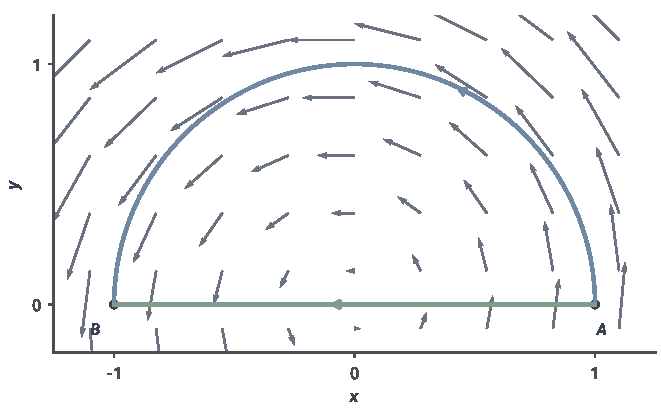
\includegraphics[width=112.0mm]{figures/00-shared/mathematical-preliminaries-upper/00-shared/matplotlib/chapter3-concept-processes/rotation-field-paths.pdf}
 \caption{灰箭头为旋转场$\bm F=(-y,x)^\top$，箭头长度统一缩放为实际场值的$1/4$。两条路径都从$A=(1,0)$到$B=(-1,0)$：蓝色上半圆与场同向，积分为$\pi$；绿色直径上场与位移垂直，积分为零。旋转场处处光滑，端点相同的两条路径上积分仍可不同；下一节说明势函数给出的路径无关条件。}
 \label{fig:analysis-process-rotation-field-paths}
\end{figure}

\section{路径无关与势函数}
\label{sec:multivariable-potential-path-independence}

重力的功只依赖起点和终点的高度，旋转场的功却依赖路线。区别在于，重力的功可以写成一个只依赖位置的量在两端的差，这个量是$-mgy$；旋转场没有这样的量。
本节把这样的量称为势函数。先说明势函数怎样把沿途累计化为端点差，再证明功与路线无关时一定能构造出势函数，最后给出可以直接检查的微分条件，并说明定义域中有洞时这个条件为何不够。

\subsection{势函数与路径积分}

\paragraph{势函数}

物理中，地面附近质量为$m$的物体在高度$y$处的重力势能为$E_{\mathrm p}(x,y)=mgy$。重力等于势能梯度的相反向量：$-\nabla E_{\mathrm p}=(0,-mg)^\top$。物体下降时势能减少，减少的势能等于重力做的功。
数学中习惯省去负号，取$\phi=-E_{\mathrm p}$，要求向量场等于某个标量函数的梯度。
\begin{definition}[势函数]
设$U\subseteq\mathbb R^d$为非空开集，$\bm F:U\to\mathbb R^d$连续。
若存在$\phi\in C^1(U)$使$\bm F=\nabla\phi$，称$\phi$为$\bm F$的\term{势函数}（potential function），称$\bm F$为梯度场，也称保守场。
\end{definition}

梯度指向函数增长最快的方向。所以在梯度非零处，梯度场的箭头指向$\phi$增大、也就是势能$-\phi$减小的方向：重力把物体拉向低处。
例如$\phi(x,y)=x^2+y^2$给出$\bm F(x,y)=(2x,2y)^\top$，箭头从原点向外，因为离原点越远$\phi$越大；常场$(1,0)^\top$的一个势函数是$\phi(x,y)=x$。

给势函数加一个常数，梯度不变，所以势函数不唯一。若$U$还是路径连通的，两个势函数只能相差一个常数。理由是：它们之差的梯度处处为零；路径连通的开集中，任意两点都能用域内折线连接；沿折线逐段使用中值公式（定理~\ref{thm:multivariable-scalar-mean-value}），可知这个差在任意两点取值相同。
这与物理中势能的零点可以任选是同一件事：把地面还是桌面取作高度零点，算出的势能差都一样。

“保守”这个名称来自能量守恒。设质量为$m$的质点在力场$\bm F=\nabla\phi$中按牛顿第二定律$m\gamma''(t)=\bm F(\gamma(t))$运动，其中$\gamma$为$C^2$路径。依次用乘积法则、运动方程和链式法则，得到
\[
 \frac{\mathrm d}{\mathrm dt}\Bigl(\tfrac12m\lVert\gamma'(t)\rVert_2^2\Bigr)
 =m\gamma''(t)^\top\gamma'(t)=\nabla\phi(\gamma(t))^\top\gamma'(t)
 =\frac{\mathrm d}{\mathrm dt}\phi(\gamma(t)),
\]
所以动能与势能之和$\frac12m\lVert\gamma'\rVert_2^2-\phi(\gamma)$的导数为零，不随时间变化。最后一个等号正是下面定理的核心：沿路径的功率$\nabla\phi^\top\gamma'$恰是$\phi\circ\gamma$的导数。

\paragraph{路径积分基本定理}

一元基本定理说，导数在区间上的积分等于原函数在两端的差。把势函数与路径复合，得到一元函数$t\mapsto\phi(\gamma(t))$。它的导数恰是第二类路径积分的被积函数，因此一元基本定理直接给出端点差。
直观上，每一小段的功$\nabla\phi^\top\Delta\bm r$近似等于$\phi$在这一小段上的增量。这些增量相加时，中间各项逐一抵消，只剩终点值减起点值。
\begin{theorem}[路径积分基本定理]
设$U\subseteq\mathbb R^d$为开集，$\phi\in C^1(U)$，$\gamma:[a,b]\to U$分段$C^1$。则
\begin{equation}
  \int_{\gamma}\nabla\phi\mathbin{\cdot}\mathrm{d}\bm{r}
  =\phi(\gamma(b))-\phi(\gamma(a)).
\label{eq:analysis-line-integral-gradient}
\end{equation}
\end{theorem}
\begin{proof}
在每个光滑参数段$[t_{j-1},t_j]$上，链式法则给出
\[
 (\phi\circ\gamma)'(t)=\nabla\phi(\gamma(t))^\top\gamma'(t).
\]
右侧是连续函数的复合与乘积，在该段上连续，所以对该段使用一元基本定理，得到
$\int_{t_{j-1}}^{t_j}\nabla\phi(\gamma(t))^\top\gamma'(t)\,\mathrm dt=\phi(\gamma(t_j))-\phi(\gamma(t_{j-1}))$。
对$j=1,\dots,n$相加，中间端点的值一正一负逐一抵消，只剩$\phi(\gamma(b))-\phi(\gamma(a))$。
\end{proof}

用势能$E_{\mathrm p}=-\phi$来读，式~\eqref{eq:analysis-line-integral-gradient}说：保守力沿任何路线做的功都等于起点势能减终点势能，即势能的下降量。示例~\ref{ex:analysis-gravity-work}的重力做功就是$\phi(x,y)=-mgy$的情形。

这个定理有两个直接推论。第一，梯度场的积分只依赖端点：端点相同的两条路线，功相同。第二，闭路径的起点与终点重合，所以梯度场沿任意闭路径的积分为零。例如把书从地上拿到桌上再放回地上，重力在全过程中做的总功为零。
方向反转时端点交换，端点差变号，这与第二类积分的方向反转性质一致。

知道势函数后，计算路径积分不必代入参数。
\begin{example}[用势函数计算沿半圆的积分]
取$\bm F=(2x,2y)^\top$，它的势函数为$\phi(x,y)=x^2+y^2$。路径取示例~\ref{ex:analysis-path-integral-comparison}中的上半圆$\gamma(t)=(\cos t,\sin t)^\top$，$0\leq t\leq\pi$，从$(1,0)$走到$(-1,0)$。由式~\eqref{eq:analysis-line-integral-gradient}，
\[
 \int_\gamma\bm F\cdot\mathrm d\bm r=\phi(-1,0)-\phi(1,0)=1-1=0.
\]
直接代入参数也得到同样结果：$\bm F(\gamma(t))^\top\gamma'(t)=2\cos t\,(-\sin t)+2\sin t\cos t=0$。这个场在圆周上处处沿半径方向，与切线垂直。
\end{example}

第二个推论还可以用来否定势函数的存在。旋转场沿单位圆逆时针一周做功$2\pi\neq0$，所以它在$\mathbb R^2$上没有势函数。

\subsection{路径无关的等价判别}

\paragraph{路径无关}

由路径积分基本定理，有势函数就有功与路线无关。要讨论反方向，先把“与路线无关”说准确。比较同一对端点之间的不同路线，需要域内任意两点都能用路径连接。对欧氏空间中的开集，路径连通时任意两点之间还能选到域内的折线，因而能选到分段光滑路径。
\begin{definition}[路径无关]
设$U\subseteq\mathbb R^d$为非空、开且路径连通的集合，$\bm F:U\to\mathbb R^d$连续。
若对任意$\bm a,\bm b\in U$及域内从$\bm a$到$\bm b$的任意两条分段$C^1$路径，第二类路径积分都相等，称$\bm F$的路径积分与路径无关。
\end{definition}

反方向的想法来自物理中定义势能的办法：选定一个参考点作为势能零点，把力从参考点到某点所做的功取负号，作为该点的势能。只有这个功与路线无关，这样定义的势能才是一个确定的数。下面的定理说明，路径无关、闭路径积分为零与势函数存在三者等价。
\begin{theorem}[路径无关的等价条件]
设$U\subseteq\mathbb R^d$非空、开且路径连通，$\bm F:U\to\mathbb R^d$连续。下列条件等价：
\begin{enumerate}
 \item 存在$\phi\in C^1(U)$使$\nabla\phi=\bm F$；
 \item $\bm F$的路径积分与路径无关；
 \item 域内每条分段$C^1$闭路径的积分都为零。
\end{enumerate}
\end{theorem}
\begin{proof}
条件1推出条件2，是路径积分基本定理的第一个推论。
条件2推出条件3：设$\gamma$是从$\bm a$出发回到$\bm a$的闭路径。停在$\bm a$不动的常值路径也从$\bm a$到$\bm a$，它的速度为零，积分为零；由路径无关，$\gamma$上的积分也为零。
条件3推出条件2：设$\gamma_1,\gamma_2$都从$\bm a$到$\bm b$。先沿$\gamma_1$走到$\bm b$，再沿$\gamma_2$的反向路径$\gamma_2^-$走回$\bm a$，拼成闭路径$\gamma_1*\gamma_2^-$。由拼接和方向反转性质，
\[
 0=\int_{\gamma_1*\gamma_2^-}\bm F\cdot\mathrm d\bm r
 =\int_{\gamma_1}\bm F\cdot\mathrm d\bm r-\int_{\gamma_2}\bm F\cdot\mathrm d\bm r.
\]

最后由条件2构造势函数。固定参考点$\bm a\in U$，对每个$\bm x\in U$，取域内任意一条从$\bm a$到$\bm x$的分段$C^1$路径，令$\phi(\bm x)$为沿它的积分。路径无关保证这个数不依赖所选路线。
下面计算偏导数。因为$U$开，存在$r>0$使以$\bm x$为中心、半径$r$的球在$U$内。对$0<|h|<r$，到$\bm x+h\bm e_j$的一条路径可以这样选：先沿原来的路径走到$\bm x$，再沿第$j$个坐标方向走线段$t\mapsto\bm x+t\bm e_j$，$t$从$0$到$h$。线段的速度为$\bm e_j$，场与速度的内积是第$j$个分量$F_j$，于是
\[
 \phi(\bm x+h\bm e_j)-\phi(\bm x)
 =\int_0^h F_j(\bm x+t\bm e_j)\,\mathrm dt.
\]
（$h<0$时按有向积分理解。）右侧除以$h$，是$F_j$在这条短线段上的平均值。$F_j$连续，$h\to0$时这个平均值趋于$F_j(\bm x)$，所以$\partial_j\phi(\bm x)=F_j(\bm x)$。
所有偏导数都等于$\bm F$的连续分量，故$\phi\in C^1(U)$且$\nabla\phi=\bm F$，得到条件1。
\end{proof}

证明中的$\phi$正是“从参考点出发做的功”。换一个参考点$\bm a'$，$\phi$只改变一个常数，即从$\bm a'$到$\bm a$的功，这与势能零点可以任选一致。

\subsection{势函数存在的微分判别}

\paragraph{交叉偏导相等的必要条件}

等价条件把势函数的存在归结为检查所有路径或所有闭路径，这无法逐条验证。我们希望找到只需对$\bm F$求导就能检查的条件。
若$\bm F=\nabla\phi$，则$F_j=\partial_j\phi$。当$\bm F$本身是$C^1$时，$\phi$具有连续的二阶偏导数，由定理~\ref{thm:multivariable-mixed-partials}，混合偏导可以交换次序，于是$\bm F$的分量之间必须满足一组关系。
\begin{theorem}[保守场的必要条件]
设$U\subseteq\mathbb R^d$为开集，$\bm F\in C^1(U;\mathbb R^d)$。
若$\bm F=\nabla\phi$，其中$\phi\in C^1(U)$，则对所有$i,j$和$\bm x\in U$，有
\[
 \partial_iF_j(\bm x)=\partial_jF_i(\bm x).
\]
\end{theorem}
\begin{proof}
由$\partial_j\phi=F_j\in C^1(U)$可知$\phi\in C^2(U)$，因此
$\partial_iF_j=\partial_i\partial_j\phi=\partial_j\partial_i\phi=\partial_jF_i$。
\end{proof}

在平面中，记$\bm F=(P,Q)^\top$，条件只有一个：$\partial_xQ=\partial_yP$。差$\partial_xQ-\partial_yP$度量向量场在一点附近的旋转程度。为看出这一点，计算沿一个小正方形边界的环流。

设正方形为$[x_0,x_0+\delta]\times[y_0,y_0+\delta]$，按逆时针方向行走。下边向右，贡献$\int_{x_0}^{x_0+\delta}P(x,y_0)\,\mathrm dx$；上边向左，贡献$-\int_{x_0}^{x_0+\delta}P(x,y_0+\delta)\,\mathrm dx$。$P$在上下两边相差约$\partial_yP\,\delta$，所以这两项之和约为$-\partial_yP\cdot\delta\cdot\delta$。同理，右边向上、左边向下，两者的贡献之和约为$\partial_xQ\cdot\delta^2$。
因此小正方形的环流约为$(\partial_xQ-\partial_yP)\,\delta^2$，即单位面积上的环流约为$\partial_xQ-\partial_yP$，下面称它为旋转率。

保守场沿每条闭路径做功为零，小正方形也不例外，所以旋转率必须处处为零，与上面的必要条件一致。这里只是近似推理；边界环流与区域内旋转率的精确关系是Green公式（定理~\ref{thm:multivariable-green}）。

两个例子可以对照。场$(2x,2y)^\top$满足$\partial_xQ=0=\partial_yP$，它确实有势函数$x^2+y^2$。旋转场$(-y,x)^\top$有$\partial_xQ-\partial_yP=1-(-1)=2\neq0$，它在每一点附近都在旋转，由上面的必要条件，它在任何非空开集上都没有势函数。这与单位圆上环流为$2\pi$的计算一致：$2\pi$恰是旋转率$2$乘单位圆盘的面积$\pi$。

\paragraph{星形域上的充分条件}

交叉偏导相等只说明每个小区域内没有旋转，是局部条件；势函数却要在整个定义域上用一个函数表示。要从局部条件得到全局结论，还需要对定义域加条件。

一个便于直接构造的条件是星形：若存在$\bm a\in U$，使从$\bm a$到每个$\bm x\in U$的整条线段都在$U$内，称$U$关于$\bm a$星形。凸开集满足这一条件，整个$\mathbb R^d$也满足。
在星形域上，可以沿用路径无关等价条件证明中“从参考点出发做功”的办法定义势函数，并且总沿直线段从$\bm a$走到$\bm x$。
\begin{theorem}[星形域上势函数的构造]
设$U\subseteq\mathbb R^d$为关于$\bm a$星形的开集，$\bm F\in C^1(U;\mathbb R^d)$，且对所有$i,j$有$\partial_iF_j=\partial_jF_i$。则
\[
 \phi(\bm x)=\int_0^1\bm F(\bm a+t(\bm x-\bm a))^\top(\bm x-\bm a)\,\mathrm dt
\]
属于$C^1(U)$且满足$\nabla\phi=\bm F$。因此$\bm F$的路径积分与路径无关。
\end{theorem}
\begin{proof}
记$\bm z=\bm x-\bm a$。$\phi(\bm x)$是$\bm F$沿线段$t\mapsto\bm a+t\bm z$，$0\leq t\leq1$，的第二类路径积分，因为这条线段的速度恒为$\bm z$。
固定$\bm x$时，这条线段是$U$内的紧集，因而它的一个足够小的紧邻域仍在$U$内；当$\bm x$在一个小范围内变动时，相应线段都留在这个紧邻域中。
$\bm F$及其一阶偏导在紧邻域上连续因而有界，所以被积函数对$x_j$的偏导数有不依赖$t$的上界，可以用式~\eqref{eq:classical-differentiate-under-integral}在积分号下对$x_j$求导。

被积函数为$\sum_iF_i(\bm a+t\bm z)z_i$。对$x_j$求导时，$z_j$对$x_j$的导数为$1$，$F_i(\bm a+t\bm z)$对$x_j$的导数由链式法则为$t\,\partial_jF_i(\bm a+t\bm z)$，所以偏导数为
\[
 F_j(\bm a+t\bm z)+t\sum_i z_i\partial_jF_i(\bm a+t\bm z).
\]
交叉偏导条件把$\partial_jF_i$换成$\partial_iF_j$，而$\sum_iz_i\partial_iF_j(\bm a+t\bm z)$正是$t\mapsto F_j(\bm a+t\bm z)$的导数，于是
\[
 \begin{aligned}
 F_j(\bm a+t\bm z)+t\sum_i z_i\partial_jF_i(\bm a+t\bm z)
 &=F_j(\bm a+t\bm z)+t\sum_i z_i\partial_iF_j(\bm a+t\bm z)\\
 &=\frac{\mathrm d}{\mathrm dt}\bigl[tF_j(\bm a+t\bm z)\bigr].
 \end{aligned}
\]
对$t$从$0$积分到$1$，由一元基本定理得$\partial_j\phi(\bm x)=1\cdot F_j(\bm a+\bm z)-0=F_j(\bm x)$。
这些偏导连续，所以$\phi\in C^1(U)$；路径无关由前一定理得到。
\end{proof}

用这个构造可以求出一个具体平面场的势函数。
\begin{example}[沿线段构造势函数$x^2y$]
取$\bm F(x,y)=(2xy,x^2)^\top$，即$P=2xy$，$Q=x^2$。它定义在整个平面上，分量都是多项式，属于$C^1$，并且$\partial_yP=2x=\partial_xQ$。整个平面关于$\bm a=\bm0$星形，代入构造公式，
\[
 \phi(x,y)=\int_0^1\bigl[2(tx)(ty)\,x+(tx)^2\,y\bigr]\,\mathrm dt
 =\int_0^13t^2x^2y\,\mathrm dt=x^2y.
\]
直接求导可验证$\nabla\phi=(2xy,x^2)^\top$。于是这个场沿任何从$(0,0)$到$(1,2)$的分段$C^1$路径做功都等于$\phi(1,2)-\phi(0,0)=2$。
\end{example}
星形域上的构造不依赖猜测：交叉偏导相等时，沿线段积分就给出势函数，任意路径上的功随之化为端点差。

\paragraph{穿孔平面上的反例}

星形域的条件不能省略。下面的向量场在原点以外处处满足交叉偏导条件，在穿孔平面上却没有势函数。
\begin{example}[穿孔平面上的涡旋场]
\label{ex:analysis-punctured-plane-vortex}
在穿孔平面$\mathbb R^2\setminus\{\bm0\}$上考虑
\[
 \bm F(x,y)=\left(-\frac{y}{x^2+y^2},\frac{x}{x^2+y^2}\right)^\top ,
\]
记它的两个分量为$P,Q$。它与旋转场$(-y,x)^\top$方向相同，都沿逆时针方向与以原点为圆心的圆相切，但大小改为到原点距离的倒数：离原点越近转得越快，类似于绕一根细涡管旋转的水流。原点处它没有定义。

先检查交叉偏导。由商的求导法则，
\[
 \begin{aligned}
 \partial_yP&=-\frac{(x^2+y^2)-y\cdot2y}{(x^2+y^2)^2}=\frac{y^2-x^2}{(x^2+y^2)^2},\\
 \partial_xQ&=\frac{(x^2+y^2)-x\cdot2x}{(x^2+y^2)^2}=\frac{y^2-x^2}{(x^2+y^2)^2},
 \end{aligned}
\]
两者在穿孔平面上处处相等，所以这个场在原点以外的每一点附近都没有旋转。

再沿单位圆$\gamma(t)=(\cos t,\sin t)^\top$，$0\leq t\leq2\pi$，逆时针走一周。在单位圆上$x^2+y^2=1$，$\bm F(\gamma(t))=(-\sin t,\cos t)^\top$与速度相同，内积为$1$，积分为$2\pi$。
闭路径积分不为零，由路径无关的等价条件，$\bm F$在穿孔平面上没有势函数。
\end{example}

局部的交叉偏导条件在这里没有给出全局的势函数。这与星形域上的定理并不矛盾：穿孔平面不是星形域，对任一点$\bm a\neq\bm0$，从$\bm a$到$-\bm a$的线段都经过原点。问题出在原点这个洞上，可以从两个角度理解。

第一，局部的势函数是极角。在不含原点的区域上，若能连续地选取点$(x,y)$的极角$\theta$，使$x=r\cos\theta$、$y=r\sin\theta$，其中$r=\sqrt{x^2+y^2}$，则直接求导可得$\nabla\theta=\bm F$。例如在右半平面$x>0$上取$\theta=\arctan(y/x)$，有$\partial_x\theta=-y/(x^2+y^2)$，$\partial_y\theta=x/(x^2+y^2)$。
在更大的区域，即去掉负半轴的平面$\mathbb R^2\setminus\{(x,0)^\top:x\leq0\}$上，取$\theta\in(-\pi,\pi)$，它连续且仍满足$\nabla\theta=\bm F$；这个区域关于$(1,0)$星形，与星形域上的定理一致。

但在整个穿孔平面上无法连续地选取极角：从$(1,0)$出发绕原点逆时针一周回到$(1,0)$，极角连续地增加了$2\pi$，起点和终点处的“势函数值”对不上。单位圆上的积分$2\pi$正是极角的这个增量。
具体地，从$(1,0)$到$(-1,0)$，沿上半圆极角从$0$增加到$\pi$，积分为$\pi$；沿下半圆$(\cos t,-\sin t)^\top$，$0\leq t\leq\pi$，极角从$0$减少到$-\pi$，积分为$-\pi$。两条路线的功相差$2\pi$，恰是绕原点一圈的积分。
不绕原点的闭路径则没有这个问题。例如以$(3,0)$为圆心、半径为$1$的圆整个落在右半平面中，那里$\theta$是势函数，沿它的积分为零。

第二，从小正方形的环流看。交叉偏导相等说明每个小正方形的环流近似为零。若一条闭路径围住的区域整个在定义域内，可以把这个区域划分成许多小正方形；相邻正方形的公共边被沿相反方向各走一次，贡献相互抵消，只剩外边界，于是外边界的环流也为零。这一推理的精确形式就是Green公式（定理~\ref{thm:multivariable-green}），它要求向量场在整个被围区域附近都有定义且连续可微。

单位圆围住的圆盘却包含原点，那里$\bm F$没有定义，无法这样填满。场在定义域内的旋转率处处为零；非零环流与被排除的原点有关。对夹在两条绕原点闭路径之间、不含原点的环形区域作同样的划分，可知两条路径上的环流相等；所以绕原点逆时针一周的简单闭路径，积分都是$2\pi$，而围住的区域不含原点的闭路径，积分为零。

相比之下，星形域上不会出现这样的洞：任何闭路径都可以沿线段向中心点$\bm a$连续收缩而不离开定义域。这从几何上解释了，为什么在星形域上交叉偏导条件已经足以保证势函数存在。

\FloatBarrier

\FloatBarrier
\section{本章小结}
\label{sec:path-integrals-chapter-summary}

路径积分沿一次行进定义，不只沿一个点集定义。参数路径同时记录经过的位置、先后次序和经过次数；同一条线段可以对应快慢不同、方向不同或来回往返的路径。分段光滑路径的弧长是内接折线长度的上确界，等于速率$\lVert\gamma'\rVert_2$的积分；一一的重参数化不改变弧长，重复行进则重复累计。

两类路径积分的被积对象和权重不同。第一类积分累计标量场，每小段的权重是长度$\mathrm ds=\lVert\gamma'(t)\rVert_2\,\mathrm dt$，结果与行进方向和快慢无关，可用来算铁丝质量和按路程的平均值。第二类积分累计向量场与有向位移的内积$\bm F(\gamma(t))^\top\gamma'(t)\,\mathrm dt$，等于切向分量的第一类积分；保向重参数化不改变它，反向行进使它变号，往返路径上的贡献相互抵消。沿闭路径的第二类积分称为环流。

功只依赖端点的条件，在路径连通开集上有三种等价表述：存在势函数$\phi$使$\bm F=\nabla\phi$，路径积分与路径无关，以及每条闭路径上的积分为零。有势函数时，路径积分基本定理把功化为端点差$\phi(\gamma(b))-\phi(\gamma(a))$。对连续可微的场，交叉偏导相等是必要条件，在星形域上也是充分条件，势函数可以沿线段积分构造出来。

定义域条件不能省略。穿孔平面上的涡旋场处处满足交叉偏导条件，绕原点一周的环流却是$2\pi$，因为局部的势函数是极角，绕原点一圈后增加$2\pi$。小正方形环流相消的推理只在被围区域整个落在定义域内时成立；它的精确形式是第~\ref{chap:integral-theorems}章的Green公式。

\par\Needspace{10\baselineskip}
\chapter{曲面积分}
\label{sec:analysis-surface-integration}
\label{chap:surface-integrals}

路径积分沿一条细线累计：线密度乘弧长得到质量，力与位移的内积累加得到功。
曲面积分把累计的范围从细线换成薄片，典型的问题有两个。
第一个问题是求一张金属薄壳的质量。已知壳上每点每平方米有多少千克，把各小片的面密度乘面积加起来即可。
第二个问题是求单位时间内有多少水穿过一张渔网。水在各点有速度，只有垂直于网面的速度分量才把水送到网的另一侧。

两个问题的被积对象不同。
第一个问题的被积对象是曲面$S$上的标量函数$h:S\to\mathbb R$，它给出每单位面积的密度，乘面积后相加得到质量、电荷等总量。
第二个问题的被积对象是向量场$\bm F:S\to\mathbb R^3$。要先取它垂直于曲面的分量，再乘面积相加，得到穿过曲面的\emph{通量}。

本章要回答：怎样度量曲面上一小片的面积，怎样按面积累计标量面密度，以及怎样在规定了穿越方向之后累计向量场穿过曲面的量。

两类积分都需要知道曲面上一小片有多大，所以第一节先用参数化求出面积元，并证明面积不依赖参数的选取。第二节按面积累计标量场，结果与曲面朝哪一侧无关。通量还要规定从哪一侧穿到哪一侧算正，所以第三节先讨论曲面的定向，再定义第二类积分，并说明法向反转、参数次序与分片相容的作用。这些积分为下一章的Gauss公式与Stokes公式准备了边界上的累计。

本章以三维欧氏空间中的曲面为主，使用第~\ref{chap:region-integrals}章的区域积分与换元公式，以及第~\ref{chap:multivariate-differentiation}章的偏导数与Jacobian。本章的参数积分都按有界Jordan区域上的Riemann积分理解；参数曲面、面积元和通量的标准构造可参考\scite{math-openstax-calculus3}。

\section{参数曲面与面积元}

平面区域的面积就是它的Jordan面积。空间中的曲面一般是弯曲的，不能不经伸缩地摊平成平面区域，所以它的面积还没有定义。

地球表面上的一点可以用经度和纬度两个数确定。这就是一种参数化：用两个参数标记曲面上的点，把曲面上的累计转回二维参数域上计算。
代价是参数域中的面积一般不等于曲面上的实际面积。经纬度网格上同样大小的格子，在赤道附近和两极附近对应的地面面积并不相同，所以每一点都要乘一个面积放大倍数来校正。
本节先说明怎样的参数化能描述一张面，再求出这个放大倍数，并证明由此得到的面积不依赖参数的选取。

\subsection{曲面的参数化}

\paragraph{正则曲面片}

曲面的参数化是一个向量值映射：输入两个实数$(u,v)$，输出空间中一点的三个坐标。并不是每个这样的映射都描述一张面。
若改变两个参数时点只沿同一个方向移动，像集可能只是一条曲线。若不同参数在一块正面积的范围内对应同一些点，按参数累计就会把这块面计算两次。
下面的定义用正则性和单次覆盖两个条件，分别排除这两种情况。

\begin{definition}[正则参数曲面片]
\label{def:analysis-regular-surface-patch}
设$E\subseteq\mathbb R^2$是有界闭区域，$E=\overline{E^\circ}$，其边界$\partial E$可用总面积任意小的有限个矩形覆盖。
设$\bm r$在$E$的一个开邻域内是$C^1$映射，写成
\[
 \bm r(u,v)=(x(u,v),y(u,v),z(u,v))^\top\in\mathbb R^3.
\]
若不同参数只有在都属于$\partial E$时才允许表示同一点，
且两个偏导向量$\bm r_u,\bm r_v$在$E^\circ$上处处线性无关，则称$\bm r$为一个正则曲面片的参数化，曲面片记为$S=\bm r(E)$。
参数边界允许产生接缝或退化点；这些边界部分按零曲面面积处理。
\end{definition}

定义中的两个偏导向量有直接的几何含义。
固定$v$而只改变$u$，点$\bm r(u,v)$在曲面上画出一条参数曲线，它的速度向量是$\bm r_u$；
固定$u$而改变$v$得到另一条参数曲线，速度向量是$\bm r_v$。
这里$\bm r_u,\bm r_v$都是三维向量，分别由三个坐标函数对同一个参数求偏导得到，并非某个标量函数的两个偏导数。

两个向量线性无关，几何上就是不共线。这时它们张成过该点的一个平面，即曲面的切平面。若这个条件不成立，像集可能根本不是一张面。

\begin{example}[像集退化为线段的参数映射]
取$E=[0,1]^2$和$\bm r(u,v)=(u+v,0,0)^\top$。
两个偏导向量都等于$(1,0,0)^\top$，因而线性相关。
当$(u,v)$取遍$E$时，$u+v$取遍$[0,2]$，所以像集是$x$轴上的线段$\{(x,0,0)^\top:0\leq x\leq2\}$。
整个正方形被压到这条线段上，像集上没有两个不共线的切方向，也没有面积可言；这个映射不满足正则性条件。
\end{example}

正则性条件排除了这种压扁的映射。
单次覆盖条件处理另一种情况：像集确实是一张面，但被参数重复计数。

\begin{example}[圆柱面的单次覆盖与二重覆盖]
\label{ex:analysis-cylinder-double-cover}
高为$1$的单位圆柱面可以写成
\[
\begin{gathered}
\bm r(\theta,z)=(\cos\theta,\sin\theta,z)^\top\\
z\in[0,1].
\end{gathered}
\]
两个偏导向量为
\[
 \bm r_\theta=(-\sin\theta,\cos\theta,0)^\top,\qquad
 \bm r_z=(0,0,1)^\top,
\]
它们处处线性无关，正则性没有问题，需要检查的只有覆盖次数。

若$\theta\in[0,2\pi]$，只有$\theta=0$与$\theta=2\pi$两条边界线表示同一条接缝，这是定义允许的。

若$\theta\in[0,4\pi]$，则对$0<\theta_0<2\pi$和$0<z<1$，点$\bm r(\theta_0,z)$同时由参数域内部的$(\theta_0,z)$和$(\theta_0+2\pi,z)$表示；
按参数累计会把整张柱面计入两次，因此这一参数域不符合定义。
\end{example}

所以，不同参数表示同一点的情形只允许出现在参数边界上，形成接缝；参数域内部的点不能与其他任何参数点表示同一点。

本章反复使用的例子是$\bm r(u,v)=(u,v,u+v)^\top$、$E=[0,1]^2$，下文称它为斜平面片。
它描述平面$z=x+y$上位于单位正方形上方的一块平行四边形，
两个切向量分别为$\bm r_u=(1,0,1)^\top$和$\bm r_v=(0,1,1)^\top$。
前两个坐标就是参数本身，所以不同参数给出不同点；两个切向量不共线，所以它满足正则曲面片的定义。

\paragraph{叉积}

要求曲面的面积，先看参数域中的一个小矩形$[u,u+\Delta u]\times[v,v+\Delta v]$被映成什么形状。
由$\bm r$的可微性，在$\Delta u,\Delta v$很小时有线性近似
\[
 \bm r(u+\Delta u,v+\Delta v)\approx\bm r(u,v)+\bm r_u\Delta u+\bm r_v\Delta v,
\]
其中$\bm r,\bm r_u,\bm r_v$都在$(u,v)$处取值。
于是小矩形的四个顶点近似映为
\[
 \bm r,\quad
 \bm r+\bm r_u\Delta u,\quad
 \bm r+\bm r_v\Delta v,\quad
 \bm r+\bm r_u\Delta u+\bm r_v\Delta v,
\]
它们正是以$\bm r_u\Delta u$和$\bm r_v\Delta v$为两边的平行四边形的顶点。
所以曲面上的小片近似是切平面内的一个小平行四边形，问题归结为：怎样由两条边向量求平行四边形的面积。

在平面上，两个边向量排成$2\times2$矩阵，其行列式的绝对值就是这个面积。
现在两条边是三维向量，排成的是$3\times2$矩阵，没有行列式可取。
三维空间中常用叉积同时记录这个面积和平行四边形所在平面的垂直方向。
对$\bm a,\bm b\in\mathbb R^3$，定义叉积
\[
 \bm a\times\bm b
 =(a_2b_3-a_3b_2,\ a_3b_1-a_1b_3,\ a_1b_2-a_2b_1)^\top.
\]
例如$(1,0,0)^\top\times(0,1,0)^\top=(0,0,1)^\top$：
$x$轴方向与$y$轴方向的单位向量张成面积为$1$的正方形，叉积是长度为$1$、沿$z$轴的向量。

后面的面积和法向计算要用到叉积的三条性质，下面逐一核对。
第一，叉积垂直于$\bm a$和$\bm b$。直接展开
\[
 \bm a^\top(\bm a\times\bm b)
 =a_1(a_2b_3-a_3b_2)+a_2(a_3b_1-a_1b_3)+a_3(a_1b_2-a_2b_1),
\]
右端六项两两抵消，结果为$0$；对$\bm b$同理。
垂直于同一平面的方向有相反的两个，叉积按右手规则选取其中之一：右手四指从$\bm a$弯向$\bm b$时，拇指指向$\bm a\times\bm b$。

第二，叉积的长度等于$\bm a,\bm b$张成的平行四边形的面积。
把两边按分量展开，可以验证Lagrange恒等式
\[
 \lVert\bm a\times\bm b\rVert_2^2
 =\lVert\bm a\rVert_2^2\lVert\bm b\rVert_2^2-(\bm a^\top\bm b)^2.
\]
记$\theta\in[0,\pi]$为两向量的夹角，则$\bm a^\top\bm b=\lVert\bm a\rVert_2\lVert\bm b\rVert_2\cos\theta$，
代入并开方（$\sin\theta\geq0$），得到
\[
 \lVert\bm a\times\bm b\rVert_2=\lVert\bm a\rVert_2\lVert\bm b\rVert_2\sin\theta.
\]
以$\bm a$为底边时，平行四边形的高是$\lVert\bm b\rVert_2\sin\theta$，所以叉积长度正是“底乘高”。
特别地，叉积为零当且仅当两向量线性相关，即平行四边形退化为线段或一点。

Lagrange恒等式的右端正是Gram矩阵
\[
 \begin{bmatrix}\bm a^\top\bm a&\bm a^\top\bm b\\\bm a^\top\bm b&\bm b^\top\bm b\end{bmatrix}
\]
的行列式，所以面积也等于两条边的Gram行列式的平方根。这种写法只用内积，不依赖叉积，也适用于高维空间中由两个向量张成的平行四边形。

第三，叉积对每个因子都是线性的，交换两个因子的次序会变号：从定义式直接看出$\bm b\times\bm a=-\bm a\times\bm b$，特别地$\bm a\times\bm a=\bm0$。
这与右手规则一致：交换次序后四指的弯曲方向相反，拇指也随之反向。

把这些性质用到小平行四边形上。由线性，
\[
 (\bm r_u\Delta u)\times(\bm r_v\Delta v)=(\bm r_u\times\bm r_v)\Delta u\Delta v;
\]
再由第二条性质，小曲面片的面积近似为
\[
 \lVert\bm r_u\times\bm r_v\rVert_2\,\Delta u\,\Delta v.
\]
因此$\lVert\bm r_u\times\bm r_v\rVert_2$就是参数化在该点的面积放大倍数：参数域中面积为$\Delta u\Delta v$的小块，
在曲面上变成面积约为这个倍数乘$\Delta u\Delta v$的小片。

同样由第二条性质，正则性条件“两个切向量线性无关”可以等价地写成$\bm r_u\times\bm r_v\ne\bm0$，即放大倍数处处为正。

平面情形可以用来核对这个倍数。若曲面就在平面$z=0$内，即$\bm r(u,v)=(x(u,v),y(u,v),0)^\top$，
则
\[
 \bm r_u\times\bm r_v=(0,0,x_uy_v-x_vy_u)^\top,
\]
其长度正是映射$(u,v)\mapsto(x,y)$的Jacobian行列式的绝对值。
这与第~\ref{sec:classical-change-variables}节换元公式中的面积权重$|\det\bm J_T|$一致；叉积长度是这个权重在三维空间中的推广。

\subsection{曲面面积的表示}

\paragraph{面积元与面积}

把参数域分成许多小矩形，由小平行四边形的面积近似，每块在曲面上的像的面积约为放大倍数乘参数面积，曲面的总面积约为这些乘积之和。
小矩形越细，线性近似越准确，求和的极限就是放大倍数在参数域上的积分。

这里直接把这个积分取作曲面面积的定义，而不像弧长那样用内接折线的上确界定义，因为曲面上的类似做法会失败。
在一段有限高的圆柱面上，可以构造顶点都在柱面上的三角形网格（称为Schwarz灯笼）：网格越来越细，三角形与柱面的夹角却不趋于零，三角形总面积可以趋于无穷。
切平面上的平行四边形则贴着曲面，不会出现这个问题。

\begin{definition}[曲面面积]
\label{def:analysis-surface-area-measure}
在单次覆盖的正则曲面片上，令$J_S=\|\bm r_u\times\bm r_v\|_2$。定义面积为
\begin{equation}
 \operatorname{area}(S)=\iint_E J_S(u,v)\,\mathrm du\,\mathrm dv.
 \label{eq:analysis-surface-area}
\end{equation}
面积元记为$\mathrm dS=J_S(u,v)\,\mathrm du\,\mathrm dv$。
\end{definition}

$J_S$在紧参数域上连续，所以积分存在。有限分片曲面的面积逐片相加；各片只沿边界接合，接缝的参数原像须能被任意小总面积的有限盒覆盖，以免重复累计。

用这一定义计算斜平面片的面积，并用初等几何核对结果。

\begin{example}[斜平面片的面积]
\label{ex:analysis-tilted-plane-area}
对斜平面片$\bm r(u,v)=(u,v,u+v)^\top$、$E=[0,1]^2$，按叉积的定义计算
\[
 \begin{aligned}
 \bm r_u\times\bm r_v
 &=(1,0,1)^\top\times(0,1,1)^\top\\
 &=(0\cdot1-1\cdot1,\ 1\cdot0-1\cdot1,\ 1\cdot1-0\cdot0)^\top
 =(-1,-1,1)^\top,
 \end{aligned}
\]
故$J_S=\lVert(-1,-1,1)^\top\rVert_2=\sqrt3$处处成立，曲面面积为
\[
 \operatorname{area}(S)=\int_0^1\int_0^1\sqrt3\,\mathrm du\,\mathrm dv=\sqrt3.
\]
用初等几何核对：两条边$\bm r_u,\bm r_v$的长度都是$\sqrt2$，内积为$1$，夹角余弦为$1/2$，即夹角为$60^\circ$；
平行四边形面积为$\sqrt2\cdot\sqrt2\cdot\sin60^\circ=\sqrt3$，与积分结果相同。
\end{example}

参数正方形的面积只有$1$，曲面片的面积却是$\sqrt3$：每个参数小块都被放大$\sqrt3$倍。
图~\ref{fig:analysis-process-surface-area-stretch}将参数小块与实际斜面小块对应起来，显示叉积长度校正的是哪一个面积。
\begin{figure*}[!htbp]
 \centering
 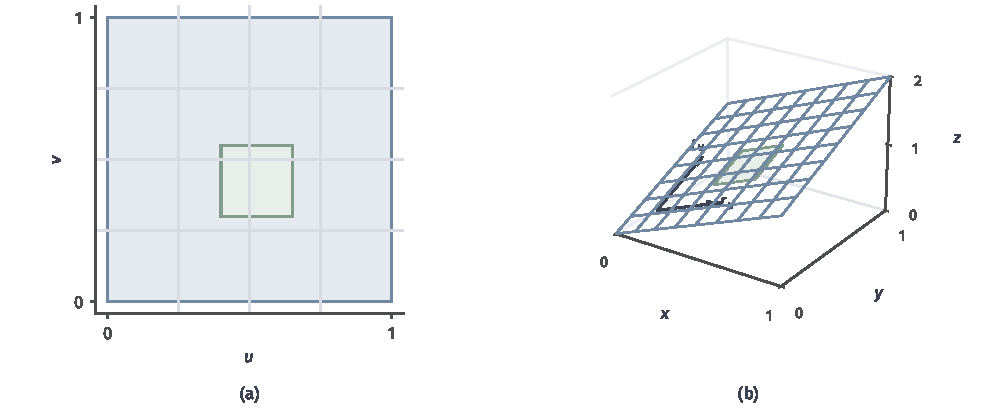
\includegraphics[width=169.0mm]{figures/00-shared/mathematical-preliminaries-upper/00-shared/matplotlib/chapter3-concept-processes/surface-area-stretch.pdf}
 \caption{参数化$r(u,v)=(u,v,u+v)^\top$把单位正方形映为斜平面片，绿色块为同一参数子区间及其像。两切向量$r_u=(1,0,1)^\top$、$r_v=(0,1,1)^\top$在右侧按$0.4$倍画出，叉积长度为$\sqrt3$。每个参数面积都放大$\sqrt3$倍，故不能把$\mathrm du\,\mathrm dv$直接当成$\mathrm dS$。}
 \label{fig:analysis-process-surface-area-stretch}
\end{figure*}

\paragraph{重参数化}

同一张面可以用不同参数标记。
面积是曲面本身的属性，不应随标记方式改变；先在斜平面片上核对一次具体的换参数。

\begin{example}[拉伸一个参数不改变面积]
\label{ex:analysis-stretched-parameter-area}
在斜平面片中令$u=2\xi$，则
\[
\begin{gathered}
\widetilde{\bm r}(\xi,v)=(2\xi,v,2\xi+v)^\top\\
(\xi,v)\in[0,1/2]\times[0,1]
\end{gathered}
\]
描述同一块平行四边形，新参数域的面积只有$1/2$。
另一方面，$\widetilde{\bm r}_\xi=(2,0,2)^\top=2\bm r_u$，$\widetilde{\bm r}_v=\bm r_v$，由叉积的线性，
\[
 \widetilde{\bm r}_\xi\times\widetilde{\bm r}_v=2(\bm r_u\times\bm r_v)=2(-1,-1,1)^\top,
\]
放大倍数为$2\sqrt3$。
因此
\[
 \int_0^1\int_0^{1/2}2\sqrt3\,\mathrm d\xi\,\mathrm dv=\sqrt3,
\]
与示例~\ref{ex:analysis-tilted-plane-area}的结果相同。
\end{example}

参数域缩小一半，每点的放大倍数恰好加倍，两者相互抵消。
下面的定理说明，这种抵消对一般的单次覆盖换参数都成立。

\begin{theorem}[重参数化下的面积元]
\label{thm:analysis-surface-reparameterization}
设$\bm r:E\to S$是正则曲面片的参数化，$T:\widetilde E\to E$是参数域之间的双射，
在$\widetilde E$的一个开邻域内为$C^1$映射，并且限制在$\widetilde E^\circ$上是到$E^\circ$的$C^1$微分同胚。
若$\widetilde{\bm r}=\bm r\circ T$仍满足曲面片条件，则
\begin{equation}
 \begin{aligned}
 \widetilde{\bm r}_\xi\times\widetilde{\bm r}_\eta
 &=\det\bm J_T\,(\bm r_u\times\bm r_v)\circ T,\\
 \widetilde J_S&=(J_S\circ T)|\det\bm J_T|.
 \end{aligned}
 \label{eq:analysis-surface-reparameterization}
\end{equation}
两组参数由此给出同一面积。
\end{theorem}

\begin{proof}
记$T(\xi,\eta)=(u(\xi,\eta),v(\xi,\eta))$。
链式法则给出
\[
 \widetilde{\bm r}_\xi=\bm r_u u_\xi+\bm r_v v_\xi,\qquad
 \widetilde{\bm r}_\eta=\bm r_u u_\eta+\bm r_v v_\eta,
\]
其中右端各量在$T(\xi,\eta)$处取值。
用叉积对每个因子的线性展开，得到四项：
\[
 \begin{aligned}
 \widetilde{\bm r}_\xi\times\widetilde{\bm r}_\eta
 &=u_\xi u_\eta(\bm r_u\times\bm r_u)+u_\xi v_\eta(\bm r_u\times\bm r_v)\\
 &\quad{}+v_\xi u_\eta(\bm r_v\times\bm r_u)\\
 &\quad{}+v_\xi v_\eta(\bm r_v\times\bm r_v).
 \end{aligned}
\]
由$\bm a\times\bm a=\bm0$，第一、四项为零；交换叉积次序会变号，即$\bm r_v\times\bm r_u=-\bm r_u\times\bm r_v$，于是第三项可与第二项合并。因此
\[
 \widetilde{\bm r}_\xi\times\widetilde{\bm r}_\eta
 =(u_\xi v_\eta-v_\xi u_\eta)(\bm r_u\times\bm r_v)\circ T,
\]
括号内正是$\det\bm J_T$，这就是第一式；两边取长度得到第二式。

把第二式在新参数域上积分，并应用经典二维换元公式，得到
\[
 \iint_{\widetilde E}(J_S\circ T)|\det DT|
 =\iint_E J_S.
\]
若换元只在参数域内部正则，先在远离边界的紧子域上应用公式，再利用连续有界权重和Jordan边界条件取极限。两组参数因而给出相同面积。
\end{proof}

几何上，这个证明把两步面积放大接在一起：新参数的小方块先由$T$映成原参数域中面积约为$|\det\bm J_T|$倍的小块，
这个小块再由$\bm r$映到曲面，面积又乘$J_S$。
二维换元公式恰好把第一步的倍数吸收掉，所以只剩下曲面本身的面积。
在示例~\ref{ex:analysis-stretched-parameter-area}中，$T(\xi,v)=(2\xi,v)$，$\det\bm J_T=2$，这正是放大倍数加倍的来源。

行列式的绝对值保证面积非负；行列式本身的符号则记录参数次序是否翻转。
例如在斜平面片上交换两个参数，令$T(\xi,\eta)=(\eta,\xi)$，即
\[
 \widetilde{\bm r}(\xi,\eta)=\bm r(\eta,\xi)=(\eta,\xi,\xi+\eta)^\top,
\]
则$\det\bm J_T=-1$，叉积由$(-1,-1,1)^\top$变为$(1,1,-1)^\top$，长度不变而方向相反。
面积不使用这个方向，后面选取通量的法向时则要用到它。

定理还要求$T$是双射。若参数在正面积的范围内重复覆盖，参数积分就会重复累计。
示例~\ref{ex:analysis-cylinder-double-cover}中，$\bm r_\theta\times\bm r_z=(\cos\theta,\sin\theta,0)^\top$，$J_S=1$；
$\theta\in[0,2\pi]$时参数积分给出柱面面积$2\pi$，$\theta\in[0,4\pi]$时却给出$4\pi$，不能当作单次覆盖的曲面面积。

\paragraph{分片曲面}

有些曲面不能用一张正则曲面片描述。单位立方体的表面由六个正方形组成，棱上没有切平面。
球面虽然可以用一张球坐标参数片覆盖（两极位于参数边界上，切向量在那里退化），也常分成上下两个半球分别处理。
本章只处理有限分片的情形：把曲面写成有限张正则曲面片的并，各片内部不重叠，交接部分在相邻曲面片中面积均为零，
整个曲面的面积由各片的面积相加。

例如立方体表面的面积就是六个单位正方形的面积之和$6$，十二条棱的面积为零，不需要在接缝上另加一项。
后面的两类曲面积分同样可以逐片计算再相加。
无界曲面，或不能这样由有限张正则曲面片覆盖的曲面，还需另外处理覆盖和可积性条件。

\section{第一类曲面积分}

有了面积，就可以回到本章开头的第一个问题：在曲面上累计一个标量密度。
这类积分只用到小片的面积，不涉及方向。

\subsection{积分的定义和可积性}

\paragraph{按面积的积分}

设一张薄金属壳占据曲面$S$，在点$\bm x$附近每单位面积的质量为$h(\bm x)$（单位如千克每平方米）。
把壳分成许多小片$S_j$，在每片内取一点$\bm x_j$。
每片很小时，片内面密度近似为常数$h(\bm x_j)$，这一片的质量约为$h(\bm x_j)\,\operatorname{area}(S_j)$。
把各片质量相加，再让分割越来越细，就得到面密度对面积的积分。带电薄壳上的电荷量、涂层表面的涂料用量都是同一种累计。

用参数表示时，每片的面积是面积元，所以把密度与面积权重相乘，再在参数域上积分。

\begin{definition}[第一类曲面积分]
\label{def:analysis-scalar-surface-integral}
设$h$是$S$上的连续标量函数，定义它的\term{第一类曲面积分}（scalar surface integral）为
\begin{equation}
 \int_Sh\,\mathrm dS
 =\iint_Eh(\bm r(u,v))J_S(u,v)\,\mathrm du\,\mathrm dv.
 \label{eq:analysis-scalar-surface-integral}
\end{equation}
右侧被积函数连续，因而积分存在且有限。
\end{definition}

式~\eqref{eq:analysis-scalar-surface-integral}右端的计算顺序是：用参数找到曲面上的点，读出该点的密度，乘该点的面积放大倍数，再在参数域上积分。
对定理~\ref{thm:analysis-surface-reparameterization}中的重参数化，把$h\circ\bm r$一并代入换元公式，可见积分值不变。

取$h=1$得到面积，取非负面密度得到质量。
例如在斜平面片上，常数密度$h=2$给出
\[
 \int_S2\,\mathrm dS=\int_0^1\int_0^1 2\sqrt3\,\mathrm du\,\mathrm dv=2\sqrt3,
\]
即面积为$\sqrt3$、每单位面积重$2$的薄片，总质量为$2\sqrt3$。

除了总量，第一类积分还给出曲面上的平均值。设$0<\operatorname{area}(S)<\infty$且$h$在$S$上连续，则
\[
 \frac1{\operatorname{area}(S)}\int_Sh\,\mathrm dS
\]
是$h$按面积加权的平均。若$h$表示地球表面各点的气温，这个量就是全球表面平均气温：
每块地面按其实际面积参与平均，而不是按经纬度网格的格子数参与平均。

第一类积分继承参数区域积分的线性、单调性和绝对值估计。有限分片曲面上逐片求和，公共接缝不另计面积。特别地，连续密度满足
\[
 \left|\int_S h\,\mathrm dS\right|\leq\sup_S|h|\operatorname{area}(S).
\]

质量和平均值都只依赖每小片的大小，面积权重又非负，与从哪一侧看曲面无关。所以把曲面的朝向反过来，第一类积分不变。

\subsection{积分的计算}

计算第一类曲面积分分三步：选一个单次覆盖的正则参数化，把$h$与参数化复合，再乘叉积的长度后在参数域上积分。
最常见的两种参数化是函数图像和球坐标。

若曲面是函数$z=\psi(x,y)$在区域$D$上的图像，其中$D$满足定义~\ref{def:analysis-regular-surface-patch}对参数域的要求，$\psi$在$D$的开邻域内为$C^1$，就可以取
$\bm r(x,y)=(x,y,\psi(x,y))^\top$。此时$\bm r_x=(1,0,\psi_x)^\top$、$\bm r_y=(0,1,\psi_y)^\top$，按叉积公式计算得
\[
 \begin{aligned}
 \bm r_x\times\bm r_y
 &=(0\cdot\psi_y-\psi_x\cdot1,\ \psi_x\cdot0-1\cdot\psi_y,\ 1\cdot1-0\cdot0)^\top\\
 &=(-\psi_x,-\psi_y,1)^\top.
 \end{aligned}
\]
叉积的第三分量恒为$1$，所以图像参数化处处正则；前两个坐标就是参数本身，所以单次覆盖也自动成立。
于是对曲面可积的$h$有
\begin{equation}
 \int_Sh\,\mathrm dS
 =\iint_Dh(x,y,\psi(x,y))\sqrt{1+\psi_x^2+\psi_y^2}\,\mathrm dx\,\mathrm dy.
 \label{eq:analysis-graph-surface-area-element}
\end{equation}

根号的几何意义如下。记$\gamma$为法向$(-\psi_x,-\psi_y,1)^\top$与$z$轴的夹角，则
\[
 \cos\gamma=\frac1{\sqrt{1+\psi_x^2+\psi_y^2}}.
\]
一块与水平面成角$\gamma$的小平面片，竖直投影到$xy$平面上时面积缩小为原来的$\cos\gamma$倍；
反过来，由投影面积$\mathrm dx\,\mathrm dy$恢复实际面积，就要除以$\cos\gamma$，即乘上这个根号。

曲面越陡，根号越大。例如$z=ax+by+c$在单位圆盘上方的部分，根号处处等于$\sqrt{1+a^2+b^2}$，面积为
$\pi\sqrt{1+a^2+b^2}$；$a=b=0$时它就是水平圆盘的面积$\pi$。

若曲面不能单值地投影到同一坐标平面，例如整张球面在每个$(x,y)$上方有两点，则需换参数化或分片。

半径$R>0$的球面可以取参数
\[
 \begin{gathered}
 \bm r(\varphi,\theta)
 =(R\sin\varphi\cos\theta,R\sin\varphi\sin\theta,R\cos\varphi)^\top,\\
 0\leq\varphi\leq\pi,\quad 0\leq\theta\leq2\pi,
 \end{gathered}
\]
其中$\varphi$是与北极方向的夹角，$\theta$是绕$z$轴转过的角度。求偏导得
\[
 \begin{aligned}
 \bm r_\varphi&=(R\cos\varphi\cos\theta,R\cos\varphi\sin\theta,-R\sin\varphi)^\top,\\
 \bm r_\theta&=(-R\sin\varphi\sin\theta,R\sin\varphi\cos\theta,0)^\top.
 \end{aligned}
\]
这两个向量的内积为零，长度分别为$R$和$R\sin\varphi$；由叉积长度公式（夹角为$\pi/2$），叉积长度为
\[
 \lVert\bm r_\varphi\times\bm r_\theta\rVert_2=R^2\sin\varphi.
\]

这个结果也可以直接看出：$\varphi$增加$\Delta\varphi$时，点沿经线走过约$R\Delta\varphi$；
$\theta$增加$\Delta\theta$时，点沿半径为$R\sin\varphi$的纬线圈走过约$R\sin\varphi\,\Delta\theta$。
小片近似为以这两个长度为边的矩形。靠近两极时纬线圈变小，同样的$\Delta\theta$对应的面积也变小。

在参数域内部$0<\varphi<\pi$、$0<\theta<2\pi$上$\sin\varphi>0$，参数化正则且单次覆盖；
两极与经线接缝来自参数边界，面积为零，不需要单独处理。
先用这个参数化求球面面积。

\begin{example}[球面的面积]
\label{ex:analysis-sphere-area}
对半径为$R$的球面，球坐标参数的面积放大倍数为$J_S=R^2\sin\varphi$，被积函数连续，可以逐次积分：
\[
 \operatorname{area}(S)
 =\int_0^{2\pi}\int_0^\pi R^2\sin\varphi\,\mathrm d\varphi\,\mathrm d\theta
 =2\pi R^2\bigl[-\cos\varphi\bigr]_0^\pi
 =4\pi R^2.
\]
\end{example}

求平均值时，面积权重同样不可缺少。下面以上半球面上的平均高度为例。

\begin{example}[上半球面的平均高度]
\label{ex:analysis-hemisphere-average-height}
取上半球面$0\leq\varphi\leq\pi/2$，高度函数$h(\bm x)=z$。
由$J_S=R^2\sin\varphi$，上半球面面积为
\[
 2\pi R^2\int_0^{\pi/2}\sin\varphi\,\mathrm d\varphi=2\pi R^2.
\]
高度函数按面积的积分为
\[
 \int_Sz\,\mathrm dS
 =\int_0^{2\pi}\int_0^{\pi/2}R\cos\varphi\cdot R^2\sin\varphi\,\mathrm d\varphi\,\mathrm d\theta
 =2\pi R^3\cdot\frac12=\pi R^3,
\]
所以按面积加权的平均高度为
\[
 \frac{\pi R^3}{2\pi R^2}=\frac R2.
\]

若改为在参数矩形$[0,\pi/2]\times[0,2\pi]$上按参数面积平均，则得到
\[
 \frac1{(\pi/2)\cdot2\pi}\int_0^{2\pi}\int_0^{\pi/2}R\cos\varphi\,\mathrm d\varphi\,\mathrm d\theta
 =\frac{2R}{\pi}\approx0.64R.
\]
\end{example}

两种平均不同，是因为同样大小的参数格子在北极附近只对应很小的面积：按参数平均会过多计入北极附近的高点，因而高估平均高度。
面积权重$R^2\sin\varphi$正是为了按实际面积而不是按参数格子求平均。

\section{第二类曲面积分}

现在回到本章开头的第二个问题：向量场穿过曲面的总量。面积只给出小片的大小；要说“穿过”，还要规定曲面的哪一侧算出发侧、哪一侧算到达侧。所以本节先讨论曲面的定向，再定义通量。

\subsection{曲面的定向}

\paragraph{单位法向量}

在正则点，切平面有两个互相相反的单位法向量，分别指向曲面的两侧。
选定其中一个，就约定：从曲面上背向它的一侧穿到它所指的一侧，算作正向穿越。
参数化的叉积给出一个自然的局部选择：在$E^\circ$上令
\begin{equation}
 \bm n(\bm r(u,v))
 =\frac{\bm r_u\times\bm r_v}{\lVert\bm r_u\times\bm r_v\rVert_2}.
 \label{eq:analysis-surface-unit-normal}
\end{equation}
由叉积的性质，这个向量长度为$1$，并且垂直于两个参数方向，即垂直于切平面；交换$u,v$的次序会把它反转。

在斜平面片上，这个公式给出$(-1,-1,1)^\top/\sqrt3$，它的第三分量为正，指向平面的上方。

在球坐标参数下，直接计算可得
\[
 \begin{aligned}
 \bm r_\varphi\times\bm r_\theta
 &=R^2\sin\varphi\,(\sin\varphi\cos\theta,\sin\varphi\sin\theta,\cos\varphi)^\top\\
 &=R\sin\varphi\,\bm r(\varphi,\theta).
 \end{aligned}
\]
在参数域内部，叉积是位置向量的正数倍，所以单位法向为$\bm r/R$，指向球的外侧。

参数边界上若叉积退化，例如球面的两极，就不用这个商定义法向；该部分面积为零，不影响通量积分。

\paragraph{定向与可定向性}

只在每一点分别选一个法向还不够。若相邻两点的法向分别指向曲面的两侧，“正向穿越”就没有一致的含义。
直观地说，给曲面定向就是给它的一侧涂上颜色，并约定法向总是从未涂色的一侧指向涂了色的一侧。沿曲面连续移动时，法向箭头不能突然跳到另一侧。

\begin{definition}[曲面的定向]
\label{def:analysis-surface-orientation}
在光滑曲面$S$上连续选取一个单位法向量场$\bm n$，称为给曲面\term{定向}（orientation）。
存在这种选择的曲面称为可定向曲面；$\bm n$和$-\bm n$给出相反的定向。
分片光滑曲面要求各片的选择相容：光滑接合处选择同一侧法向，
折角处按整个曲面的同一侧约定，但不要求接缝上存在唯一法向。
\end{definition}

常见曲面都可以定向。函数图像可以选第三分量为正的向上法向；
球面可以选外法向$\bm x/R$，此时涂色的一侧是外表面。
闭曲面把空间分成内外两部分；当它围成一个规则区域时，通常选取指向区域外侧的外法向，第~\ref{sec:multivariable-boundary-relations}节的散度定理也采用这一约定。
立方体表面是分片曲面，六个面各自选指向立方体外的法向，这些选择在棱处都属于外侧，因而相容。

并非所有曲面都能定向，典型的例子是Möbius带：把一条长纸带扭转半圈，再把两端粘在一起。
一只蚂蚁从某点出发，沿纸带中线爬一圈，始终不跨过纸带边缘；回到出发位置时，它却站在出发时的背面。想只涂纸带的一面，沿中线一直涂下去，最后两面都会被涂上颜色。
用参数可以把这一现象写成具体计算。

\begin{example}[Möbius带上的法向绕行一圈后反向]
\label{ex:analysis-mobius-normal-reversal}
取
\[
 \begin{gathered}
 \bm r(u,v)=\bigl(\lambda\cos u,\ \lambda\sin u,\ \tfrac v2\sin\tfrac u2\bigr)^\top,\\
 \lambda=1+\tfrac v2\cos\tfrac u2,\\
 0\leq u\leq2\pi,\quad -1\leq v\leq1.
 \end{gathered}
\]
$u$绕中心圆走一圈，$v$在纸带的宽度方向变化；绕行一圈时宽度方向只转过半圈，所以$\bm r(2\pi,v)=\bm r(0,-v)$，参数边界$u=0$与$u=2\pi$被反向粘在一起。

在中线$v=0$上，两个偏导向量为
\[
 \begin{aligned}
 \bm r_u&=(-\sin u,\cos u,0)^\top,\\
 \bm r_v&=\tfrac12\bigl(\cos\tfrac u2\cos u,\ \cos\tfrac u2\sin u,\ \sin\tfrac u2\bigr)^\top,
 \end{aligned}
\]
于是
\[
 \begin{aligned}
 \bm N(u)&=\bm r_u\times\bm r_v\\
 &=\tfrac12\bigl(\cos u\sin\tfrac u2,\ \sin u\sin\tfrac u2,\ -\cos\tfrac u2\bigr)^\top,
 \end{aligned}
\]
它的长度恒为$1/2$。
$u=0$时它是$\frac12(0,0,-1)^\top$，$u=2\pi$时它是$\frac12(0,0,1)^\top$，而两者对应同一点$\bm r(0,0)=\bm r(2\pi,0)=(1,0,0)^\top$。

假设$\bm n$是Möbius带上连续的单位法向场。
在中线上的点$\bm r(u,0)$处，$\bm n$与$2\bm N(u)$都是单位法向，只能相等或相反。记
\[
 \varepsilon(u)=2\bm n(\bm r(u,0))^\top\bm N(u)\in\{1,-1\}.
\]
$\varepsilon$在$[0,2\pi]$上连续且只取$\pm1$，所以是常数。
但$\bm n(\bm r(0,0))=\bm n(\bm r(2\pi,0))$而$\bm N(2\pi)=-\bm N(0)$，从而$\varepsilon(2\pi)=-\varepsilon(0)$，矛盾。
因此Möbius带上不存在连续的单位法向场。
\end{example}

Möbius带的面积仍可按面积计算，第一类积分也有定义，因为它们不使用法向。
但“水从哪一侧流到哪一侧”在Möbius带上没有全局一致的含义，所以这里按全局定向定义的通量不适用于它。

\subsection{积分的定义和可积性}

\paragraph{通量积分}

先看最简单的情形。设水以恒定速度$\bm v$流动，一块面积为$A$的平面网放在水中，选定单位法向$\bm n$。
在时间$\Delta t$内，恰好贴在网面上的水滴各自移动$\bm v\Delta t$，这段时间内穿过网的水因此充满一个斜柱体：
底面就是这块网，侧棱是向量$\bm v\Delta t$。
斜柱体的体积等于底面积乘高，高是侧棱在$\bm n$方向上投影的长度$|\bm v^\top\bm n|\Delta t$。
给这个体积加上符号，沿$\bm n$方向穿过记为正，就得到单位时间内沿$\bm n$方向穿过网的水量
\[
 \frac{A\,(\bm v^\top\bm n)\Delta t}{\Delta t}=(\bm v^\top\bm n)\,A.
\]

这个公式区分了三种情形。
水流平行于网面时，$\bm v^\top\bm n=0$，斜柱体被压扁成没有体积的薄片：水沿着网面滑过，没有水穿过网。
水流沿$\bm n$方向垂直于网面时，$\bm v^\top\bm n=\lVert\bm v\rVert_2$，同样流速下穿过的水最多。
水逆着$\bm n$流动时，$\bm v^\top\bm n<0$，结果为负，表示水沿$-\bm n$方向穿过；把法向换成$-\bm n$，同一股水流的结果就变号。
总之，只有速度的法向分量$\bm v^\top\bm n$起作用，切向分量对穿过的水量没有贡献。

下面用一块倾斜的正方形核对这个公式，并比较竖直流与沿着正方形的流。

\begin{example}[竖直流与切向流穿过倾斜正方形]
\label{ex:analysis-tilted-square-flux}
设$0\leq\alpha\leq\pi/2$，倾斜的单位正方形为
\[
\begin{gathered}
\bm r(u,v)=(u\cos\alpha,\ v,\ u\sin\alpha)^\top\\
(u,v)\in[0,1]^2,
\end{gathered}
\]
它与水平面的夹角为$\alpha$。
由$\bm r_u=(\cos\alpha,0,\sin\alpha)^\top$和$\bm r_v=(0,1,0)^\top$，计算得
\[
 \bm r_u\times\bm r_v=(-\sin\alpha,0,\cos\alpha)^\top.
\]
它的长度为$1$，所以这块面的面积为$1$。单位法向为
\[
 \bm n=(-\sin\alpha,0,\cos\alpha)^\top ,
\]
其第三分量非负。

先看竖直向上的恒定流$\bm F=(0,0,c)^\top$。它的法向分量为$\bm F^\top\bm n=c\cos\alpha$，按平面网的公式，通量为
\[
 (\bm F^\top\bm n)\cdot1=c\cos\alpha.
\]
例如$c=2$、$\alpha=60^\circ$时通量为$1$，只是水平放置（$\alpha=0$）时通量$2$的一半：正方形越倾斜，迎着水流的部分越少。

再看沿正方形本身方向的流$\bm F=(\cos\alpha,0,\sin\alpha)^\top=\bm r_u$。这时
\[
 \bm F^\top\bm n=-\sin\alpha\cos\alpha+\sin\alpha\cos\alpha=0,
\]
水只沿着面滑过，通量为零。
\end{example}

竖直流的通量$c\cos\alpha$也等于流速$c$乘这块面在水平面上的投影面积：正方形投影为矩形$[0,\cos\alpha]\times[0,1]$，面积为$\cos\alpha$。
所以对竖直落下的雨，倾斜屋顶接到的雨量只取决于屋顶的水平投影。
切向流的结果则说明，沿曲面流动的场不穿过曲面。

对弯曲的曲面和随位置变化的场，把曲面分成小片$S_j$，在片内取点$\bm x_j$。
每片近似为平面，场在片内近似为常向量$\bm F(\bm x_j)$，所以由平面网的公式，这一片的通量约为$\bm F(\bm x_j)^\top\bm n(\bm x_j)\,\operatorname{area}(S_j)$。
各片相加并让分割变细，得到标量函数$\bm F^\top\bm n$对面积的积分。
$\bm F$不必是流速：电场的通量、热流密度的通量都按同样方式定义，分别描述电场穿过曲面的通量与单位时间穿过的热量。

\begin{definition}[第二类曲面积分]
\label{def:analysis-surface-flux-integral}
设可定向曲面$S$已选定单位法向$\bm n$，向量场$\bm F:S\to\mathbb R^3$连续。
定义\term{第二类曲面积分}（flux integral），也称通量积分，为
\begin{equation}
 \int_S\bm F^\top\bm n\,\mathrm dS
 =\iint_E\bm F(\bm r(u,v))^\top(\bm r_u\times\bm r_v)\,\mathrm du\,\mathrm dv,
 \label{eq:analysis-surface-flux}
\end{equation}
其中参数化的叉积方向须与所选$\bm n$一致；若方向相反，右端需乘$-1$。
分片曲面的通量按相容定向逐片相加。
\end{definition}

式~\eqref{eq:analysis-surface-flux}右端没有出现叉积的长度，因为单位法向的分母与面积元中的长度恰好抵消：
\[
 \bm n\,\mathrm dS
 =\frac{\bm r_u\times\bm r_v}{\lVert\bm r_u\times\bm r_v\rVert_2}\,\lVert\bm r_u\times\bm r_v\rVert_2\,\mathrm du\,\mathrm dv
 =(\bm r_u\times\bm r_v)\,\mathrm du\,\mathrm dv.
\]
向量$(\bm r_u\times\bm r_v)\,\mathrm du\,\mathrm dv$同时记录了小片的面积（它的长度）和朝向（它的方向），称为有向面积元。
计算通量时只需把场与有向面积元作内积，不必先求单位法向。

通量为正，表示沿所选法向穿过的量多于逆法向穿过的量；为负则相反。
曲面上不同部分的贡献可以正负抵消，所以通量是净穿过量。

通量是一个标量，不能与把向量场$\bm F=(P,Q,R)^\top$的三个分量分别作面积积分所得的向量
\[
 \Bigl(\int_SP\,\mathrm dS,\ \int_SQ\,\mathrm dS,\ \int_SR\,\mathrm dS\Bigr)^\top
\]
混为一谈：后者不使用法向，也不随定向改变。

若$\bm F=(P,Q,R)^\top$，常把有向面积元的三个分量记为
\[
 \bm n\,\mathrm dS=(\mathrm dy\,\mathrm dz,\mathrm dz\,\mathrm dx,\mathrm dx\,\mathrm dy)^\top,
\]
从而把通量写为
\[
 \int_SP\,\mathrm dy\,\mathrm dz+Q\,\mathrm dz\,\mathrm dx+R\,\mathrm dx\,\mathrm dy.
\]

每个分量是小片在相应坐标平面上的有向投影面积。
以第三分量$n_3\,\mathrm dS$为例：记$\gamma$为法向与$z$轴的夹角，小片投影到$xy$平面时面积乘$|\cos\gamma|=|n_3|$，$n_3$的符号则记录法向朝上还是朝下。
示例~\ref{ex:analysis-tilted-square-flux}中倾斜正方形的$\mathrm dx\,\mathrm dy$分量为$\cos\alpha\,\mathrm du\,\mathrm dv$，正是它的水平投影面积。
因此$R\,\mathrm dx\,\mathrm dy$累计的是场的$z$分量穿过水平投影的量，另外两项同理；这些记号中的$\mathrm dx\,\mathrm dy$带有符号，不同于区域积分中的面积元。

图~\ref{fig:analysis-process-normal-projection}在一个法向截面内分解场值，说明通量只累计哪一部分。
\begin{figure}[!htbp]
 \centering
 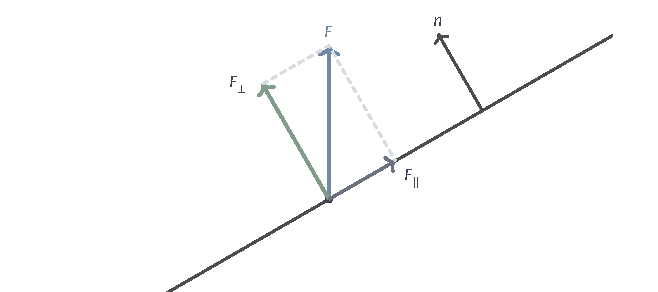
\includegraphics[width=112mm]{figures/00-shared/mathematical-preliminaries-upper/00-shared/tikz/chapter3-concept-processes/normal-projection.pdf}
 \caption{黑斜线表示局部切平面的一个截面，$n$为所选单位法向。向量$F$分为$F_\perp=(F^\top n)n$与切向部分$F_\parallel$；通量使用有符号标量$F^\top n$乘面积，切向部分不贡献。将$n$改为$-n$时标量分量变号，但投影向量$F_\perp$不变，这与直接把场反向不同。}
 \label{fig:analysis-process-normal-projection}
\end{figure}

连续向量场在紧曲面上有界，参数化的有向面积元也连续，所以每片上的通量都存在。

\subsection{积分的性质}

以下运算都在同一曲面、同一法向约定下进行，向量场都假设连续。
通量是标量函数$\bm F^\top\bm n$的面积积分，所以线性和可加性直接沿用第一类积分的性质；与方向有关的法向反转和重参数化需要单独说明。

\paragraph{线性}

向量场相加或数乘以后，法向分量也相应地相加或数乘：$(\bm F+\bm G)^\top\bm n=\bm F^\top\bm n+\bm G^\top\bm n$，$(c\bm F)^\top\bm n=c(\bm F^\top\bm n)$。因此
\[
 \begin{aligned}
 \int_S(\bm F+\bm G)^\top\bm n\,\mathrm dS
 &=\int_S\bm F^\top\bm n\,\mathrm dS+\int_S\bm G^\top\bm n\,\mathrm dS,\\
 \int_S(c\bm F)^\top\bm n\,\mathrm dS
 &=c\int_S\bm F^\top\bm n\,\mathrm dS.
 \end{aligned}
\]
两股水流叠加后穿过网的水量，等于两股水流分别穿过的水量之和；流速加倍，穿过的水量也加倍。这里缩放的是场，曲面的法向约定保持不变。

\paragraph{曲面分割的可加性}

将$S$分为内部不重叠的有限片$S_1,\ldots,S_N$，并在每片采用原定向的限制，则
\[
 \int_S\bm F^\top\bm n\,\mathrm dS
 =\sum_{j=1}^N\int_{S_j}\bm F^\top\bm n\,\mathrm dS.
\]
零面积的接缝不贡献积分。关键在于每片沿用原来的法向：若某片单独反转法向，这一片计入的是反方向的穿越量，加起来就不再是整张曲面的通量。

\paragraph{法向反转}

在场和曲面不变时，把$\bm n$换成$-\bm n$会使通量变号：
\[
 \int_S\bm F^\top(-\bm n)\,\mathrm dS
 =-\int_S\bm F^\top\bm n\,\mathrm dS.
\]
水流本身没有变，变的只是计数方向。例如原法向朝上时，从下往上的穿越原来记为正，现在记为负。第一类积分不使用法向，换定向不改变结果，这是两类积分的区别。

\paragraph{重参数化}

更换参数时，所选的几何法向保持不变。
由定理~\ref{thm:analysis-surface-reparameterization}，新参数的叉积等于原叉积乘$\det\bm J_T$，
而二维换元公式使用的是$|\det\bm J_T|$。若$\det\bm J_T>0$，两者相同，式~\eqref{eq:analysis-surface-flux}右端不变；
若$\det\bm J_T<0$，例如交换两个参数，新叉积指向相反一侧，按定义中“方向相反时乘$-1$”的约定校正后，结果仍不变。
因此，固定曲面定向并完成这一校正后，通量只依赖曲面、定向和场，与参数的选择无关。

\subsection{积分的计算}

计算通量分三步：先确定要用哪一侧的法向，再选一个叉积指向该侧的参数化（若指向相反，就在结果前加负号），最后在参数域上累计$\bm F$与有向面积元的内积。

对于图像曲面$z=\psi(x,y)$，第一类积分的计算中已经求出叉积
\[
 \bm r_x\times\bm r_y=(-\psi_x,-\psi_y,1)^\top,
\]
它的第三分量为正，指向上方。
因此取向上法向时，对$\bm F=(P,Q,R)^\top$有
\begin{equation}
 \int_S\bm F^\top\bm n\,\mathrm dS
 =\iint_D(-P\psi_x-Q\psi_y+R)(x,y,\psi(x,y))\,\mathrm dx\,\mathrm dy.
 \label{eq:analysis-graph-surface-flux}
\end{equation}
取向下法向则在右侧加负号。这一式直接使用有向面积元，叉积的长度已经与单位法向的分母抵消，不能再额外乘一次$\sqrt{1+\psi_x^2+\psi_y^2}$。

斜平面片是$\psi(x,y)=x+y$在单位正方形上的图像，可以用它核对通量与投影面积的关系。

\begin{example}[斜平面片上的竖直通量]
\label{ex:analysis-tilted-plane-flux}
取斜平面片$\bm r(u,v)=(u,v,u+v)^\top$、$E=[0,1]^2$和向上单位法向$(-1,-1,1)^\top/\sqrt3$。
对竖直单位场$\bm F=(0,0,1)^\top$，用有向面积元计算，场与参数叉积$(-1,-1,1)^\top$的内积为$1$，故
\[
 \int_S\bm F^\top\bm n\,\mathrm dS
 =\int_0^1\int_0^1 1\,\mathrm du\,\mathrm dv=1.
\]
也可以把面积和法向分量分开计算：这块面的面积为$\sqrt3$（示例~\ref{ex:analysis-tilted-plane-area}），场的法向分量处处为$\bm F^\top\bm n=1/\sqrt3$，两者相乘仍为$1$。这个值恰好是斜平面片在$xy$平面上的投影面积。
\end{example}

同样地，平面$z=ax+by+c$在单位圆盘$D$上方的部分对该场的向上通量为$\iint_D1\,\mathrm dx\,\mathrm dy=\pi$，
等于水平投影面积；它的实际面积则为$\pi\sqrt{1+a^2+b^2}$。
这与示例~\ref{ex:analysis-tilted-square-flux}中倾斜屋顶接雨的结果一致：竖直的流只“看见”曲面的水平投影。

对半径为$R$的球面，讨论单位法向量时已算出$(\varphi,\theta)$次序的参数叉积为$R\sin\varphi\,\bm r$，它在参数域内部指向外侧。
下面三个例子都取外法向，依次计算径向场、点源场和恒定场的通量。

\begin{example}[径向场穿过球面]
\label{ex:analysis-radial-field-sphere-flux}
令$\bm F(\bm x)=\bm x/R$。在球面上$\bm F$恰等于外单位法向，$\bm F^\top\bm n=1$，由示例~\ref{ex:analysis-sphere-area}，
\[
 \int_S\bm F^\top\bm n\,\mathrm dS
 =\int_S1\,\mathrm dS=4\pi R^2.
\]
取内法向时通量为$-4\pi R^2$。
\end{example}

这次外向通量与面积相等，是因为法向分量处处为$1$。
一般情形下$|\bm F^\top\bm n|\leq\lVert\bm F\rVert_2$，通量的绝对值不超过场的大小对面积的积分；场的方向偏离法向时，只有法向分量计入通量。

接下来的两个例子形成对比：一个场由原点处的点源发出，另一个场在空间中处处相同。

\begin{example}[点源场的通量与半径无关]
\label{ex:analysis-point-source-sphere-flux}
令$\bm F(\bm x)=\bm x/\lVert\bm x\rVert_2^3$（$\bm x\neq\bm0$），$S$是以原点为中心、半径为$R$的球面，外法向为$\bm n=\bm x/R$。
$\bm F$在不含原点的球面上连续，因而法向分量可积。
在$S$上$\lVert\bm x\rVert_2=R$，故
\[
 \bm F^\top\bm n=\frac{\bm x^\top\bm x}{R^3\cdot R}=\frac1{R^2},
\]
外向通量为$(1/R^2)\cdot4\pi R^2=4\pi$。
\end{example}

球面越大，场越弱，但面积增大的倍数恰好抵消场的减弱，所以通量不随$R$改变：
以点源为中心的球面无论多大，测得的点源单位时间放出的总量都一样。

\begin{example}[恒定场穿过球面的净通量为零]
\label{ex:analysis-constant-field-sphere-flux}
令$\bm F=(0,0,1)^\top$。由$\bm r_\varphi\times\bm r_\theta=R\sin\varphi\,\bm r$，被积函数为
\[
 \bm F^\top(\bm r_\varphi\times\bm r_\theta)=R\sin\varphi\cdot R\cos\varphi=R^2\sin\varphi\cos\varphi,
\]
于是
\[
 \int_S\bm F^\top\bm n\,\mathrm dS
 =\int_0^{2\pi}\int_0^\pi R^2\sin\varphi\cos\varphi\,\mathrm d\varphi\,\mathrm d\theta=0.
\]
分开计算，上半球面$0\leq\varphi\leq\pi/2$的外向通量为
\[
 2\pi R^2\int_0^{\pi/2}\sin\varphi\cos\varphi\,\mathrm d\varphi=\pi R^2,
\]
下半球面$\pi/2\leq\varphi\leq\pi$的外向通量为$-\pi R^2$。
\end{example}

在恒定场中，水从下半球面流入球内，又从上半球面等量流出；球内既不产生也不吸收水，所以闭曲面的净通量为零。包围点源的球面则有正的净通量。
可见闭曲面的净通量反映它所围区域内部的源与汇。第~\ref{sec:multivariable-boundary-relations}节将用区域内部的散度累计来计算闭曲面的通量，并核对这里的几个结果。

\FloatBarrier

\FloatBarrier
\section{本章小结}
\label{sec:surface-integrals-chapter-summary}

曲面积分先要解决面积的度量。正则参数曲面片用两个参数标记曲面上的点，两条切向量$\bm r_u,\bm r_v$张成切平面；参数小矩形近似映为以$\bm r_u\Delta u,\bm r_v\Delta v$为边的平行四边形，面积放大倍数是叉积长度$\lVert\bm r_u\times\bm r_v\rVert_2$，也等于两切向量Gram行列式的平方根。

面积直接定义为这个倍数的参数积分，内接三角形的上确界在曲面上会失败。正则性排除被压扁的参数化，单次覆盖排除重复计数；合法的换参数使叉积乘上$\det\bm J_T$，面积因而不变。参数边界上的接缝或退化点（例如球坐标的两极）只是参数的奇异，不是曲面本身的奇异，面积为零，不影响积分。

第一类曲面积分按面积累计标量面密度，权重$\mathrm dS$非负，结果与参数化和曲面的定向都无关。按面积平均与按参数平均不同：上半球面的平均高度按面积是$R/2$，按经纬度格子是$2R/\pi$。函数图像的面积元是$\sqrt{1+\psi_x^2+\psi_y^2}\,\mathrm dx\,\mathrm dy$，球面的是$R^2\sin\varphi\,\mathrm d\varphi\,\mathrm d\theta$。

第二类曲面积分累计向量场的法向分量$\bm F^\top\bm n$，先要给曲面连续地选定一侧的单位法向；Möbius带不存在这样的选择，因而没有全局的通量。参数公式使用有向面积元$(\bm r_u\times\bm r_v)\,\mathrm du\,\mathrm dv$，叉积的方向须与所选法向一致，否则乘以$-1$；交换参数次序会反转叉积。法向反转使通量变号，分片曲面要求各片法向相容，封闭曲面通常取外法向。

几个球面例子显示了通量的含义：点源场的外向通量与半径无关，恒定场穿过闭球面的净通量为零。闭曲面的净通量反映所围区域内部的源与汇，这正是下一章Gauss公式要精确表达的关系；有边界的定向曲面则通过诱导方向与边界环流联系，由Stokes公式表达。

\chapter{积分定理}
\label{chap:integral-theorems}

一元微积分基本定理说，$f'$在区间上的积分等于$f$在两个端点上的值之差：内部各点的变化率累计起来，只剩下边界上的信息。前两章分别在路径和曲面上累计了向量场的切向分量与法向分量，得到环流与通量。本章要回答：对平面区域、空间区域和有边界的曲面，内部的哪种导数累计起来恰好等于边界上的环流或通量；这样的等式在什么条件下成立，能用来做什么。

第一节先回答“内部的哪种导数”。把向量场看作流体的速度场，散度是一点附近单位体积的净流出，旋度沿某个方向的分量是垂直于该方向的单位面积环流；两者都由收缩小立方体、小正方形上的通量和环流求极限得到。Laplace算子是梯度的散度，比较函数在一点的值与周围平均值，并与梯度、散度、旋度之间的恒等式一起，为后面的分部积分准备材料。

第二节把局部关系拼成整体关系。把对象切成小块，每块上导数乘大小近似等于边界上的累计；相邻小块的公共边界被沿相反方向各算一次而抵消，只剩外边界。按这一机制依次得到平面区域上的Green公式、空间区域上的Gauss公式和有边界曲面上的Stokes公式，再由Gauss公式推出多元分部积分与Green恒等式。

使用这些公式时要分清几种条件：边界取正向、外法向还是由曲面法向诱导的方向；向量场是否在整个积分对象附近连续可微；边界项能否因边界条件而消失。本章使用第~\ref{chap:region-integrals}章的区域积分与累次积分，第~\ref{chap:path-integrals}章的环流与势函数，第~\ref{chap:surface-integrals}章的通量与定向，以及第~\ref{chap:multivariate-differentiation}章的Jacobian、Hessian与混合偏导数的交换。

\section{局部微分算子}
\label{sec:multivariable-differential-operators}

欧氏坐标下，标量函数的梯度就是一阶偏导数排成的列向量（式~\eqref{eq:multivariable-gradient-coordinates}）。对向量场，各分量一阶偏导数的适当组合也给出有几何含义的量。设$\bm F$是开集$U$上的向量场，不妨把它想成流体的速度场：$\bm F(\bm x)$是流体在位置$\bm x$处的速度。

对这样的场有两个自然的局部问题：在一点附近，流体是净流出还是净流入；流体是否绕这一点打转。
两个问题的答案都由$\bm F$各分量的一阶偏导数决定，只是用到的组合不同：回答前者的是散度，回答后者的是旋度。

最后的Laplace算子作用于标量函数，比较函数在一点的值与周围平均值的差别。这三个算子都是下一节积分公式中的内部量。

\subsection{散度与局部通量}

\paragraph{小立方体的净流出}

设$\bm F=(F_1,F_2,F_3)^\top$是三维流体的速度场。由第~\ref{sec:analysis-surface-integration}章，单位时间穿过面积为$\Delta S$、单位法向为$\bm n$的一小片曲面的流体体积约为$(\bm F^\top\bm n)\Delta S$。
现在以点$\bm a$为中心取边长为$h$的小立方体，各面与坐标平面平行，估计单位时间从它流出的净体积。

先看与$x$轴垂直的两张面。右面$x=a_1+h/2$的外法向是$\bm e_1$，场在这张面上的法向分量是$F_1$；用面中心的值代表整张面，流出量约为$F_1(\bm a+\tfrac h2\bm e_1)h^2$。
左面$x=a_1-h/2$的外法向是$-\bm e_1$，流出量约为$-F_1(\bm a-\tfrac h2\bm e_1)h^2$；$F_1>0$时这个量为负，表示沿$x$正方向的流动在左面是流入。两面合计为
\[
 \Bigl[F_1\bigl(\bm a+\tfrac h2\bm e_1\bigr)-F_1\bigl(\bm a-\tfrac h2\bm e_1\bigr)\Bigr]h^2
 \approx \partial_1F_1(\bm a)\,h\cdot h^2,
\]
这里用偏导数乘距离$h$近似$F_1$在两张面中心之间的差。
若$F_1$沿$x$方向增大，右面流出的比左面流入的多，这对面贡献正的净流出；若$F_1$沿$x$方向不变，流入与流出恰好相等。

另外两对面同样分别给出约$\partial_2F_2(\bm a)h^3$和$\partial_3F_3(\bm a)h^3$。六张面合计后除以体积$h^3$，得到
\[
 \frac{\text{小立方体的净流出}}{\text{小立方体的体积}}
 \approx\partial_1F_1(\bm a)+\partial_2F_2(\bm a)+\partial_3F_3(\bm a).
\]

这个近似可以变成极限。$\bm F$连续可微时，可以在整个小立方体上把它展开为$\bm F(\bm a)+D\bm F(\bm a)(\bm x-\bm a)+o(h)$。每张面的面积为$h^2$，所以余项对六张面通量的总贡献是$o(h^3)$。常数项在相对的两面上抵消，线性项给出上面的三个偏导数。除以$h^3$再令$h\to0$，净流出与体积之比的极限就是上式右侧。这一步只用到局部展开，不需要整个区域上的Gauss公式。
右侧的偏导数之和称为散度。
\begin{definition}[散度]
\label{def:multivariable-divergence}
设$U\subseteq\mathbb R^d$为开集，$\bm F=(F_1,\ldots,F_d)^\top:U\to\mathbb R^d$的各分量一阶偏导数存在。
$\bm F$的\term{散度}（divergence）是标量函数
\begin{equation}
 \operatorname{div}\bm F
 =\nabla\mathbin{\cdot}\bm F
 =\sum_{j=1}^d\partial_jF_j.
 \label{eq:multivariable-divergence}
\end{equation}
\end{definition}
当$\bm F$可微时，这个和也等于Jacobian矩阵$D\bm F$的迹。它只累计对应坐标方向的变化率；非对角偏导数不直接进入净流出率。

\paragraph{源的强度}

由小立方体上的推导，散度是单位体积的净流出率，可以理解为一点处源的强度。
$\operatorname{div}\bm F(\bm a)>0$表示$\bm a$附近像有一个源，流体在这里产生并向外流走；$\operatorname{div}\bm F(\bm a)<0$表示这里像一个汇，流入的多于流出的；散度为零表示流入与流出平衡。
若流体不可压缩，内部又没有注入或抽出流体的源和汇，则每个小体积的流入量都等于流出量，速度场的散度处处为零。

下面三个场分别对应均匀膨胀、绕轴转动和整体平移，可以用来检验这一解释。
\begin{example}[径向场、旋转场与常场的散度]
三维径向场$\bm F(x,y,z)=(x,y,z)^\top$满足$\partial_xF_1=\partial_yF_2=\partial_zF_3=1$，所以$\operatorname{div}\bm F=1+1+1=3$：流体从各处均匀地向外膨胀，每单位体积每单位时间多出$3$个单位体积的流体。

旋转场$\bm G(x,y,z)=(-y,x,0)^\top$的第一分量不含$x$，第二分量不含$y$，第三分量为零，所以$\operatorname{div}\bm G=0+0+0=0$：流体绕$z$轴转动，任何小立方体流入多少就流出多少。

常场$\bm H=(1,0,0)^\top$的各分量都是常数，散度同样为$0$：流体整体平移，每个小立方体从左面流入的量都从右面流出。
\end{example}
旋转场和常场都不是零场，散度却都为零。散度为零只表示局部净流出率为零，不表示向量场为零。

二维场$(P,Q)^\top$的散度相应为$P_x+Q_y$，它是小正方形四条边上的净流出除以面积所得的极限；定理~\ref{thm:multivariable-planar-flux}的平面通量公式使用这一标量函数。

\subsection{旋度与局部环流}

\paragraph{小正方形上的环流}

净流出不能描述绕一点的旋转。
旋转场$\bm G=(-y,x,0)^\top$的散度为零，但在水平平面内沿以$z$轴上一点为圆心的圆周逆时针走一圈，场始终与行进方向相同，环流不为零。
度量一点附近的旋转，要用小闭路径上的环流。先在平面上计算小正方形边界的环流。

设平面场为$(P,Q)^\top$，以$\bm a$为中心取边长为$h$的正方形，沿逆时针方向走一圈。

下边从左向右，切向分量是$P$，贡献约$P(\bm a-\tfrac h2\bm e_2)h$；上边从右向左，贡献约$-P(\bm a+\tfrac h2\bm e_2)h$。用偏导数乘距离$h$近似两边中心处$P$的差，两者合计
\[
 \Bigl[P\bigl(\bm a-\tfrac h2\bm e_2\bigr)-P\bigl(\bm a+\tfrac h2\bm e_2\bigr)\Bigr]h
 \approx-\partial_yP(\bm a)h^2.
\]

右边从下向上，贡献约$Q(\bm a+\tfrac h2\bm e_1)h$；左边从上向下，贡献约$-Q(\bm a-\tfrac h2\bm e_1)h$。同样地，两者合计
\[
 \Bigl[Q\bigl(\bm a+\tfrac h2\bm e_1\bigr)-Q\bigl(\bm a-\tfrac h2\bm e_1\bigr)\Bigr]h
 \approx\partial_xQ(\bm a)h^2.
\]
四边相加后除以面积$h^2$，得到
\[
 \frac{\text{小正方形边界的逆时针环流}}{\text{小正方形的面积}}
 \approx\partial_xQ(\bm a)-\partial_yP(\bm a).
\]
两项的符号可以这样理解。若$Q$沿$x$方向增大，右边向上的流速比左边大，这一对边推动逆时针转动；若$P$沿$y$方向增大，上边向右的流速比下边大，这一对边推动顺时针转动，所以$\partial_yP$带负号。

在三维空间中，小正方形可以放在分别垂直于三个坐标轴的平面里，行进方向都取从相应坐标轴正方向看的逆时针。
垂直于$z$轴时，平面坐标是$(x,y)$，$(F_1,F_2)$相当于$(P,Q)$，同样的计算给出$\partial_xF_2-\partial_yF_1$；
垂直于$x$轴时，平面坐标的次序是$(y,z)$，$(F_2,F_3)$相当于$(P,Q)$，得到$\partial_yF_3-\partial_zF_2$；
垂直于$y$轴时，平面坐标的次序是$(z,x)$，$(F_3,F_1)$相当于$(P,Q)$，得到$\partial_zF_1-\partial_xF_3$。
这样选取坐标次序，是因为$\bm e_2\times\bm e_3=\bm e_1$、$\bm e_3\times\bm e_1=\bm e_2$：从坐标轴正方向看，第一个平面坐标轴逆时针转过直角得到第二个。
把这三个环流率按$x,y,z$轴的次序排成一个向量，就得到旋度。
\begin{definition}[旋度]
\label{def:multivariable-curl}
设$U\subseteq\mathbb R^3$为开集，$\bm F=(F_1,F_2,F_3)^\top:U\to\mathbb R^3$的各分量一阶偏导数存在。
$\bm F$的\term{旋度}（curl）是向量场
\begin{equation}
 \operatorname{curl}\bm F=\nabla\times\bm F
 =\begin{pmatrix}
   \partial_yF_3-\partial_zF_2\\
   \partial_zF_1-\partial_xF_3\\
   \partial_xF_2-\partial_yF_1
  \end{pmatrix}.
 \label{eq:multivariable-curl}
\end{equation}
\end{definition}

\paragraph{旋转的轴与强度}

坐标平面上的三个计算可以推广到任意方向。

设$\bm F$连续可微，$\bm n$是单位向量；在过点$\bm a$且垂直于$\bm n$的平面内，取以$\bm a$为中心的小正方形或小圆周，从$\bm n$的箭头一侧看按逆时针行进。
尺寸趋于零时，环流除以所围面积的极限等于$(\operatorname{curl}\bm F)(\bm a)^\top\bm n$。
$\bm n$为坐标轴方向时，这就是上面的计算；一般方向的证明放在Stokes公式之后。

由Cauchy--Schwarz不等式，$(\operatorname{curl}\bm F)^\top\bm n\leq\lVert\operatorname{curl}\bm F\rVert_2$；旋度不为零时，等号当且仅当$\bm n$与旋度同向时成立。
所以旋度的方向是局部旋转最强的转轴，其长度是旋转的强度；转向由右手定则确定：右手大拇指沿旋度方向，其余四指弯曲的方向就是转向。

一个物理图像是放进流水中的小桨轮。让桨轮的转轴沿$\bm n$，水流沿轮缘推动各个叶片。桨轮是否转动、往哪边转，取决于沿轮缘的环流，也就是$(\operatorname{curl}\bm F)^\top\bm n$的符号；转轴与旋度平行时转得最快。这一图像帮助理解定义，但不代替上面的计算。

先用整体转动和径向膨胀检验这一图像。
\begin{example}[刚体旋转与径向膨胀的旋度]
\label{ex:analysis-rigid-rotation-curl}
整体以角速度$\omega$绕$z$轴旋转的流体，速度场为$\bm F=\omega(-y,x,0)^\top$。代入定义，前两个分量$\partial_yF_3-\partial_zF_2$与$\partial_zF_1-\partial_xF_3$都为零，第三个分量为
\[
 \partial_x(\omega x)-\partial_y(-\omega y)=2\omega,
\]
所以$\nabla\times\bm F=(0,0,2\omega)^\top$。
特别地，$\omega=1/2$时$\bm F=(-y/2,x/2,0)^\top$，旋度为$(0,0,1)^\top$。

径向场$(x,y,z)^\top$的第$i$个分量只依赖第$i$个坐标，旋度定义中的每个交叉偏导数都为零，所以旋度为零：流体只向外膨胀而不打转。
\end{example}
刚体旋转的旋度沿转轴，长度是角速度的两倍，与桨轮图像一致。不过，旋度与流线是否弯曲并不是一回事，下面两个场从相反的方向说明这一点。
\begin{example}[剪切流与涡旋场]
剪切流$\bm F=(y,0,0)^\top$的流线都是水平直线。它的偏导数中只有$\partial_yF_1=1$不为零，所以$\nabla\times\bm F=(0,0,-1)^\top$。
物理上，上方的水比下方的水向右流得快，桨轮的上缘被推得更多，从$z$轴正方向看桨轮顺时针转动，与第三分量为负一致。

再看平面上沿同心圆流动的场。

设流体在每个以原点为圆心的圆周上逆时针流动，半径为$r$的圆周上速率为$s(r)>0$，其中$s$可微，即
\[
 \begin{gathered}
(P,Q)^\top=g(r)\,(-y,x)^\top\\
g(r)=\frac{s(r)}r\\
r=\sqrt{x^2+y^2}>0.
 \end{gathered}
\]
由$\partial_xr=x/r$、$\partial_yr=y/r$，有
\[
 Q_x=g(r)+\frac{g'(r)x^2}r,\qquad
 P_y=-g(r)-\frac{g'(r)y^2}r,
\]
所以
\[
 Q_x-P_y=2g(r)+rg'(r)=\frac{s(r)}r+s'(r).
\]
第一项$s(r)/r$来自流线的弯曲，第二项$s'(r)$来自不同半径上流速的差别。刚体旋转$s(r)=\omega r$时两项都等于$\omega$，合计$2\omega$，与前例一致。

第~\ref{sec:multivariable-potential-path-independence}节穿孔平面上的涡旋场$(-y,x)^\top/(x^2+y^2)$对应$s(r)=1/r$，两项分别为$1/r^2$与$-1/r^2$，所以在原点以外$Q_x-P_y=0$。
\end{example}
剪切流的流线是直线，旋度却不为零；涡旋场的流线弯曲，在原点以外旋度却为零。后者的原因是：流线弯曲带来的逆时针倾向，恰好被外侧流速较慢带来的顺时针倾向抵消，所以放在原点以外的小桨轮不转。

对二维场$(P,Q)^\top$，平面内需要的是标量$Q_x-P_y$。
把二维场补上为零的第三分量，写成三维场$(P,Q,0)^\top$后，这一标量正是旋度的第三分量，也就是旋度在向上法向$\bm e_3$上的分量。
符号$\nabla\mathbin\cdot$和$\nabla\times$表示这里定义的偏导数组合，不是两个普通数值向量的内积或叉积。

图~\ref{fig:analysis-process-divergence-circulation-fields}在同一个单位圆周上分别观察净流出与切向环流，比较两种微分算子所记录的信息。
\begin{figure*}[!htbp]
 \centering
 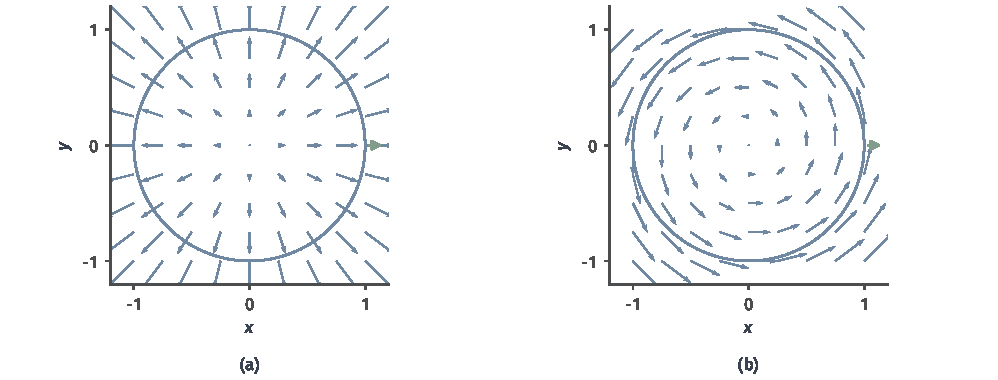
\includegraphics[width=169.0mm]{figures/00-shared/mathematical-preliminaries-upper/00-shared/matplotlib/chapter3-concept-processes/divergence-circulation-fields.pdf}
 \caption{(a) 径向场$(x,y)^\top$的二维散度为$2$、旋转率$Q_x-P_y=0$，圆周外向通量为$2\pi$、环流为零。(b) 旋转场$(-y,x)^\top$的散度为零、旋转率为$2$，通量为零、环流为$2\pi$。绿箭头仅标记外法向；蓝色场箭头按相同常数缩放。零散度不等于零场，也不等于零环流。}
 \label{fig:analysis-process-divergence-circulation-fields}
\end{figure*}

\subsection{Laplace算子与微分恒等式}

标量函数的梯度是向量场，可以对它再取散度，把各坐标方向的二阶变化相加。这一复合运算出现在多元分部积分中，也出现在描述热传导和扩散的方程中。
\begin{definition}[Laplace算子]
\label{def:multivariable-laplacian}
对开集$U\subseteq\mathbb R^d$上的二阶连续可微标量函数$v$，定义\term{Laplace算子}（Laplacian）为
\begin{equation}
 \Delta v=\operatorname{div}(\nabla v)
 =\sum_{j=1}^d\partial_j^2v.
 \label{eq:multivariable-laplacian}
\end{equation}
\end{definition}
梯度把标量函数变为向量场，散度再把向量场变为标量函数，所以$\Delta v$仍是标量函数；它与输入、输出都是向量场的旋度属于不同类型的运算。

从矩阵表示看，$\Delta v$也是Hessian矩阵的迹。例如$v(\bm x)=\|\bm x\|_2^2$的Hessian为$2\bm I$，所以$\Delta v=2d$。

由混合偏导数可以交换次序，梯度、散度和旋度之间有两条恒等式。在三维开集上，若$v\in C^2$，则
\[
 \operatorname{curl}(\nabla v)=\bm0.
\]
例如第三分量是$\partial_x\partial_yv-\partial_y\partial_xv=0$，另两个分量同理。反过来，由旋度为零推出势函数存在，还要核对定义域，星形域与有孔域的区别已在第~\ref{sec:multivariable-potential-path-independence}节说明。

若向量场$\bm F\in C^2$，则
\[
 \operatorname{div}(\operatorname{curl}\bm F)=0.
\]
将旋度的三个分量代入散度，得到六个二阶混合偏导数，每一项都与交换求导次序后的另一项异号相消。

注意对象类型：第一个等式的输入是标量函数，结果是零向量；第二个的输入是向量场，结果是数零。

\paragraph{与邻域平均值的差}

一元情形中，$v''(a)>0$表示函数在$a$附近向上弯，$v(a)$低于两侧邻点的平均值。多元情形可以做同样的比较。

在$\bm a$的每个坐标方向上各取前后两个邻点$\bm a\pm h\bm e_j$，沿该坐标作二阶Taylor展开：
\[
 v(\bm a+h\bm e_j)+v(\bm a-h\bm e_j)-2v(\bm a)=h^2\partial_j^2v(\bm a)+o(h^2),
\]
一阶项$\pm h\partial_jv(\bm a)$在两点相加时抵消。对$j=1,\ldots,d$求和，再除以邻点个数$2d$，得到
\[
 \frac1{2d}\sum_{j=1}^d\bigl[v(\bm a+h\bm e_j)+v(\bm a-h\bm e_j)\bigr]-v(\bm a)
 =\frac{h^2}{2d}\Delta v(\bm a)+o(h^2).
\]
因此，$h$足够小时，$\Delta v(\bm a)>0$表示$v(\bm a)$低于周围邻点的平均值，$\Delta v(\bm a)<0$表示高于平均值；$\Delta v(\bm a)=0$表示二者之差是$o(h^2)$，在这一精度下相等。

下面用两个二次函数直接比较邻点平均值与中心值。
\begin{example}[二次函数的邻点平均]
取$v(x,y,z)=x^2+y^2+z^2$，则$\Delta v=2+2+2=6$。在原点，$v(\bm0)=0$；六个邻点$\pm h\bm e_j$上的值都是$h^2$，所以邻点平均值比中心值高$h^2$，恰等于
\[
 \frac{h^2}{2d}\Delta v=\frac{h^2}6\cdot6=h^2.
\]
二次函数的Taylor展开没有余项，等式精确成立。

再取$v(x,y)=x^2-y^2$，则$\Delta v=2-2=0$。原点的四个邻点$(\pm h,0)$与$(0,\pm h)$上的取值为$h^2,h^2,-h^2,-h^2$，平均值恰为$0=v(\bm0)$。
\end{example}
第二个函数在$x$方向向上弯、在$y$方向向下弯，两种弯曲正好抵消。Laplace算子记录的是各坐标方向弯曲的总和，不能据此判断每个方向各自怎样弯曲。

\paragraph{热传导中的含义}

设$u(t,\bm x)$是时刻$t$物体内位置$\bm x$处的温度，它对$\bm x$二阶连续可微。热量从高温处流向低温处，Fourier热传导定律把单位时间穿过单位面积的热流写成$\bm q=-k\nabla u$，其中常数$k>0$为导热系数，$\nabla$只作用于空间变量$\bm x$\scite{math-openstax-calculus3}。
由散度的含义，单位体积的热量净流出率为
\[
 \operatorname{div}\bm q=-k\Delta u.
\]
没有热源时，单位体积内热量的增加率等于净流入率
\[
 -\operatorname{div}\bm q=k\Delta u;
\]
再除以单位体积的热容$c>0$，得到温度的变化率
\begin{equation}
 \partial_tu=\frac kc\,\Delta u,
 \label{eq:multivariable-heat-equation}
\end{equation}
这就是热传导方程。

比周围平均更冷的点满足$\Delta u>0$，会从周围吸收热量而升温；比周围平均更热的点满足$\Delta u<0$，会降温。温度分布因而逐渐被抹平。

温度不再随时间变化时，处处有$\Delta u=0$；由邻域平均的公式，每点的温度在上述精度下等于周围的平均。这里的Fourier定律是物理模型，本节只用它说明$\Delta$的含义。

\section{区域与边界的积分关系}
\label{sec:multivariable-boundary-relations}

一元微积分基本定理说，若$f$在$[a,b]$上连续可微，则$f'$在区间上的积分等于$f(b)-f(a)$：区间内部各点的变化率累计起来，只剩下两个端点上的函数值。
区间的边界就是这两个端点，所以$f(b)-f(a)$也可以读成带符号的边界求和：右端点记正号，左端点记负号。
路径积分基本定理（式~\eqref{eq:analysis-line-integral-gradient}）把同样的关系搬到路径上：梯度场沿路径的积分，等于势函数在终点与起点的值之差。

本节把“内部导数的累计等于边界上的累计”推广到平面区域、空间区域和曲面，分别得到Green公式、Gauss公式和Stokes公式。
三种推广的思路相同。先把对象切成许多小块；在每个小块上，某个导数乘小块的大小，近似等于向量场沿小块边界的累计。相邻两块的公共边界被两块各算一次，两次方向相反，相加后抵消，最后只剩下整个对象的外边界。

内部量与边界量要配对使用。沿边界的环流累计向量场的切向分量，对应的内部量是旋度；穿过边界的通量累计向量场的法向分量，对应的内部量是散度。
本节先规定边界的方向，再依次给出三个公式，最后由Gauss公式推出多元分部积分与Green恒等式。经典公式的组织参考向量微积分教材\scite{math-openstax-calculus3}。

\paragraph{边界的定向}

将一个区域分成相邻小块时，公共边或公共面不属于原区域的外边界。要使这些内部贡献相消，各小块必须采用相容的方向，而且要与小块上局部计算所用的方向一致：环流按逆时针计算，通量按外法向计算。下面依次规定平面区域边界的行进方向、区域边界的外法向，以及定向曲面边界的行进方向。

\paragraph{平面区域的正向边界}

平面区域的边界是路径，所以先规定沿边界行进的方向。本节考虑的平面区域，边界由若干条简单闭曲线组成；简单闭曲线指除首尾相合外不自交的闭曲线。
对有界平面区域，取边界方向使沿曲线前进时区域总在左侧，称为正向边界。沿单位圆逆时针行走，单位圆盘始终在左手边，所以圆盘的正向边界是逆时针方向。

有孔洞时，外边界仍是逆时针；围绕孔洞的内边界要使区域而非孔洞留在左侧，因而是顺时针。
例如圆环$1<x^2+y^2<4$的外圈$r=2$逆时针、内圈$r=1$顺时针，两圈边界方向相反。
这个约定与小块相消的要求一致：把圆环切成许多小块，每块都按逆时针走边界，内部公共边相互抵消后，剩在孔洞边上的那些边恰好被顺时针走过。

边界由多段光滑弧组成时，按这一方向逐段相接，转角处不另加积分项。一般地，相邻平面小块各自采用正向边界时，公共边被沿相反方向走过，两个有向路径积分恰好抵消。

\paragraph{区域边界的外法向}

通量需要的是法向，而不是边界的行进方向。空间区域的外单位法向从内部指向外部；有孔洞时，孔洞边界的外法向指向孔洞。
例如球壳$1<\lVert\bm x\rVert_2<2$在外球面上的外法向背离原点，在内球面上的外法向指向原点。
相邻子区域的公共面上，两侧子区域的外法向相反，所以内部通量相消。

平面区域边界上的外单位法向按同样方式规定，只是通量沿边界按弧长累计。
外法向与正向边界的单位切向量$\bm\tau=(\tau_1,\tau_2)^\top$有固定关系：区域在行进方向的左侧，外侧就在右侧，所以把$\bm\tau$顺时针转过直角就得到外法向$\bm n=(\tau_2,-\tau_1)^\top$。
例如在单位圆的点$(1,0)$处，逆时针的切向量是$(0,1)^\top$，按此公式得到$(1,0)^\top$，确实指向圆外。

\paragraph{定向曲面边界的诱导方向}

曲面取定单位法向$\bm n$后，边界路径的方向就不能再任意选择。边界的正向按右手约定确定：右手大拇指朝法向，其余四指弯曲的方向为正向，称为由法向诱导的方向，简称诱导方向。
等价地，沿边界前进并把头朝向法向时，曲面留在左侧。面朝前进方向$\bm f$、头顶朝$\bm u$站立时，左手方向是$\bm u\times\bm f$；用这个叉积可以核对具体例子。

下面用这个叉积核对两张以单位圆为边界的曲面，后面检验Stokes公式时会用到它们。
\begin{example}[向上圆盘与外向上半球面的诱导方向]
\label{ex:analysis-hemisphere-induced-orientation}
对取向上法向$\bm e_3$的单位圆盘，在边界点$(1,0,0)$处取前进方向$\bm f=\bm e_2$，左手方向为$\bm e_3\times\bm e_2=-\bm e_1$，指向圆盘内部。所以诱导方向是从上方看逆时针。

对取外法向的上半单位球面，赤道上的点$(1,0,0)$处外法向是$\bm e_1$。同样取前进方向$\bm f=\bm e_2$，左手方向为$\bm e_1\times\bm e_2=\bm e_3$，正指向半球面所在的上方。所以它的诱导方向也是从上方看逆时针，与向上圆盘的边界方向相同。
\end{example}
两张曲面在边界点处的法向不同，曲面伸出的方向也不同；但二者都满足“头朝法向时曲面在左侧”，所以诱导出同一个边界方向。

翻转曲面法向，边界的诱导方向也随之翻转。分片曲面的定向相容，是指相邻曲面片在公共边上诱导出相反的行进方向。这时公共边上的路径积分相消，只留下整张曲面的真正边界。

图~\ref{fig:analysis-process-boundary-orientation-cancellation}把相容方向的作用画出来：只有内部公共边相消，才会只剩下整个对象的外边界。
\begin{figure}[!htbp]
 \centering
 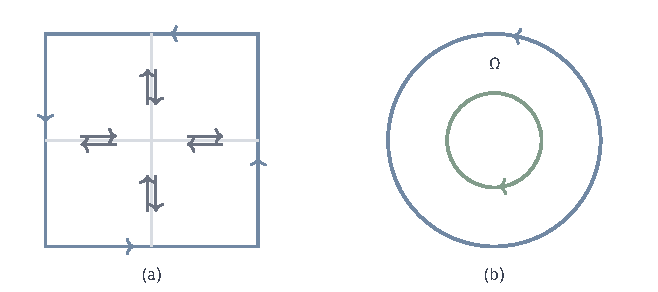
\includegraphics[width=112mm]{figures/00-shared/mathematical-preliminaries-upper/00-shared/tikz/chapter3-concept-processes/boundary-orientation-cancellation.pdf}
 \caption{(a) 四个小正方形各取逆时针正向，共同边被沿相反方向走过；灰箭头略错开以便辨认，实际是同一条边。相加后只留下蓝色外边界。(b) 圆环的外边界逆时针、孔洞边界顺时针，沿任一边界前进时区域均在左侧。曲面拼片时也按公共边相反方向保证Stokes边界项相消。}
 \label{fig:analysis-process-boundary-orientation-cancellation}
\end{figure}

\subsection{Green公式与平面边界}

平面区域的边界是一维路径。对同一个二维向量场，可以沿边界累计切向分量，得到环流；也可以累计外法向分量，得到通量。两种边界积分分别对应区域内部的$Q_x-P_y$和散度$P_x+Q_y$。

\subsubsection{Green公式的环流形式}

旋度一节在小正方形上算出：逆时针环流约等于$Q_x-P_y$乘正方形面积。
把区域$\Omega$划分成许多小正方形（靠近弯曲边界处是不规则的小块），对每块写出这一近似再相加。
相邻两块的公共边在两块中方向相反，贡献抵消，剩下的只有沿$\Omega$正向边界的环流；另一侧各块“$Q_x-P_y$乘面积”之和，则是区域积分的近似和。
Green公式说明，在适当条件下这一近似在加细后成为精确等式：区域内各处微小旋转的累计，等于沿边界走一圈的总环流。
\begin{theorem}[Green公式]
\label{thm:multivariable-green}
设$\Omega\subseteq\mathbb R^2$为有界开区域，边界由有限条分段$C^1$简单闭曲线组成，
且区域在每段光滑边界附近位于边界的一侧。边界取正向，即外边界逆时针、孔洞边界顺时针。
若二维向量场$\bm F=(P,Q)^\top$在$\overline\Omega$的开邻域内连续可微，则\term{Green公式}（Green's theorem）给出
\begin{equation}
 \oint_{\partial\Omega}P\,\mathrm dx+Q\,\mathrm dy
 =\iint_\Omega\left(\frac{\partial Q}{\partial x}-\frac{\partial P}{\partial y}\right)\,\mathrm dx\,\mathrm dy.
 \label{eq:multivariable-green}
\end{equation}
\end{theorem}
左侧是向量场的切向路径积分，右侧是标量函数$Q_x-P_y$的区域积分。在矩形上，这个等式可以直接由一元基本定理和累次积分公式推出。
\begin{proof}[矩形情形的证明]
取$\Omega=(a,b)\times(c,d)$，先写出左侧沿四条边的贡献。
水平边上$\mathrm dy=0$，竖直边上$\mathrm dx=0$，所以$Q$只在竖直边出现，$P$只在水平边出现。
下边$(t,c)$、$a\leq t\leq b$从左向右，上边从$(b,d)$走到$(a,d)$，两条水平边的贡献分别为
\[
 \int_a^bP(x,c)\,\mathrm dx,\qquad -\int_a^bP(x,d)\,\mathrm dx.
\]
右边从下向上，左边从上向下，两条竖直边的贡献分别为
\[
 \int_c^dQ(b,y)\,\mathrm dy,\qquad -\int_c^dQ(a,y)\,\mathrm dy.
\]

再看右侧。场在闭矩形附近连续可微，以下被积函数均可积。固定$x$，对$y$用一元基本定理得
\[
 \int_c^d\partial_yP(x,y)\,\mathrm dy=P(x,d)-P(x,c);
\]
再对$x$积分，并由连续函数的累次积分公式换成区域积分。对$Q$则先固定$y$、对$x$积分。于是
\[
 \begin{aligned}
 -\iint_\Omega\partial_yP\,\mathrm dx\,\mathrm dy
 &=\int_a^b[P(x,c)-P(x,d)]\,\mathrm dx,\\
 \iint_\Omega\partial_xQ\,\mathrm dx\,\mathrm dy
 &=\int_c^d[Q(b,y)-Q(a,y)]\,\mathrm dy.
 \end{aligned}
\]
第一行恰是下边与上边的两项，第二行恰是右边与左边的两项。
四项合起来，正是沿下、右、上、左四条边逆时针行进得到的路径积分。
\end{proof}
有限个矩形拼接时，公共边上的积分因方向相反而抵消。
一般规则区域的证明还需处理区域分片及边界逼近误差，不能仅凭小矩形上的等式完成；这里引用一般形式，完整论证可参考向量微积分教材\scite{math-strang1991calculus}。

先用旋转场在单位圆盘上核对公式两侧，并观察边界方向的作用。
\begin{example}[旋转场在单位圆盘上的Green公式]
\label{ex:analysis-rotation-field-green-disk}
取$\bm F=(P,Q)^\top=(-y,x)^\top$，$\Omega$为单位圆盘。$\bm F$在整个平面上连续可微，定理条件满足。
右侧被积函数为$Q_x-P_y=1-(-1)=2$，区域积分为$2\cdot\pi=2\pi$。

左侧取逆时针边界$\gamma(t)=(\cos t,\sin t)^\top$，$0\leq t\leq2\pi$，则
\[
 \bm F(\gamma(t))^\top\gamma'(t)=\sin^2t+\cos^2t=1 ,
\]
积分同样为$2\pi$。
若把圆周改为顺时针，左侧变为$-2\pi$，右侧仍为$2\pi$，等式不再成立。
\end{example}
区域积分不含方向信息，边界积分却随方向反转而变号；Green公式的符号由正向边界的约定决定。

Green公式也可以反过来使用：选一个满足$Q_x-P_y\equiv1$的场，右侧就是区域的面积，于是面积可以由边界环流算出。
\begin{example}[用边界计算面积]
\label{ex:analysis-green-area-formula}
设$\Omega$满足定理~\ref{thm:multivariable-green}的条件。取$P=-y/2$、$Q=x/2$，则$Q_x-P_y=1$，Green公式给出
\begin{equation}
 \operatorname{area}(\Omega)=\frac12\oint_{\partial\Omega}x\,\mathrm dy-y\,\mathrm dx.
 \label{eq:analysis-green-area-formula}
\end{equation}

对半轴为$\alpha,\beta>0$的椭圆区域，正向边界取$\gamma(t)=(\alpha\cos t,\beta\sin t)^\top$、$0\leq t\leq2\pi$。这时$\mathrm dx=-\alpha\sin t\,\mathrm dt$、$\mathrm dy=\beta\cos t\,\mathrm dt$，
\[
 x\,\mathrm dy-y\,\mathrm dx=(\alpha\beta\cos^2t+\alpha\beta\sin^2t)\,\mathrm dt=\alpha\beta\,\mathrm dt,
\]
所以面积为$\frac12\cdot2\pi\alpha\beta=\pi\alpha\beta$。
\end{example}
这个公式只需要沿边界走一圈、记录坐标与位移，就能得到所围面积；机械求积仪正是按这一原理工作的。

定理要求场在$\overline\Omega$的开邻域内连续可微。区域包含场的奇点时，这一条件不再满足，下面的例子说明它不能省略。
\begin{example}[有孔区域上的涡旋场]
\label{ex:analysis-annulus-vortex-green}
第~\ref{sec:multivariable-potential-path-independence}节的穿孔平面反例中，$\bm F=(-y,x)^\top/(x^2+y^2)$在原点以外满足$Q_x-P_y=0$，但沿单位圆逆时针一周的环流为$2\pi$。

取圆环$\Omega=\{1<x^2+y^2<4\}$。它的闭包不含原点，$\bm F$在$\overline\Omega$的一个开邻域内连续可微，Green公式适用，右侧为$0$。
左侧由两圈组成。外圈$r=2$逆时针，参数化为$(2\cos t,2\sin t)^\top$，此时$\bm F=(-\sin t,\cos t)^\top/2$，与速度$(-2\sin t,2\cos t)^\top$的内积为$1$，环流为$2\pi$。

内圈$r=1$按正向取顺时针，环流为$-2\pi$。两者相加为零，与右侧一致。
\end{example}
外圈逆时针为$2\pi$、内圈顺时针为$-2\pi$，也就是说，两条圆周按同一逆时针方向走时，环流都是$2\pi$。环流来自原点处的奇点，而不是来自圆环内部。
单位圆盘含有原点，$\bm F$在那里无定义，不满足Green公式的条件，所以不能由$Q_x-P_y=0$推出单位圆上的环流为零。

\subsubsection{Green公式的通量形式}

现在把平面向量场想成薄层流体的速度场，考察单位时间有多少流体穿过区域边界流出。每个小正方形的净流出约等于散度乘面积。相邻两块的公共边上外法向相反，一块的流出就是另一块的流入，相加后抵消。因此可以预期，区域内部源强度的总和等于穿过边界的净流出。

计算通量需要把场投影到外法向上。正向边界的有向位移是$\bm\tau\,\mathrm ds=(\mathrm dx,\mathrm dy)^\top$，而外法向由$\bm\tau$顺时针转过直角得到，因此
\[
 \bm n\,\mathrm ds=(\mathrm dy,-\mathrm dx)^\top.
\]
这一关系把法向通量写成切向路径积分，从而可以使用Green公式。
\begin{theorem}[平面区域的通量公式]
\label{thm:multivariable-planar-flux}
在与Green公式相同的区域条件下，若$\bm F=(F_1,F_2)^\top$在$\overline\Omega$的开邻域内连续可微，
$\bm n$是边界的外单位法向，则
\begin{equation}
 \int_{\partial\Omega}\bm F^\top\bm n\,\mathrm ds
 =\iint_\Omega\operatorname{div}\bm F\,\mathrm dx\,\mathrm dy.
 \label{eq:multivariable-planar-flux}
\end{equation}
\end{theorem}
\begin{proof}
利用外法向与正向边界的关系，$\bm F^\top\bm n\,\mathrm ds=F_1\,\mathrm dy-F_2\,\mathrm dx$，所以左侧等于
\[
 \oint_{\partial\Omega}(-F_2)\,\mathrm dx+F_1\,\mathrm dy.
\]
在Green公式中取$(P,Q)=(-F_2,F_1)$，右侧被积函数为$Q_x-P_y=\partial_xF_1+\partial_yF_2=\operatorname{div}\bm F$。
\end{proof}
这也是二维的散度公式。它与环流形式使用相同的区域条件，但累计的边界分量和内部导数不同。

下面在单位圆盘上比较两个场的通量：一个从各处均匀发散，一个只绕原点打转。
\begin{example}[单位圆盘上径向场与旋转场的通量]
取$\bm F(x,y)=(x,y)^\top$，$\Omega$为单位圆盘。散度为$1+1=2$，区域积分为$2\pi$。
边界参数化为$\gamma(t)=(\cos t,\sin t)^\top$，$0\leq t\leq2\pi$，外法向$\bm n=\gamma(t)$，$\mathrm ds=\mathrm dt$，且
\[
 \bm F^\top\bm n=\cos^2t+\sin^2t=1,
\]
所以边界通量也为$2\pi$。若改取内法向，通量变为$-2\pi$。

再取旋转场$\bm G=(-y,x)^\top$。它的散度为$0+0=0$；在单位圆上$\bm G^\top\bm n=-y\cdot x+x\cdot y=0$，通量为零，两侧一致。它的环流却是示例~\ref{ex:analysis-rotation-field-green-disk}算出的$2\pi$。
\end{example}
径向场好比流体在圆盘内各处均匀产生，产生的总量全部从圆周流出。旋转场则像杯中被搅动的水：水在杯中打转，却没有流出杯壁。通量与环流记录的是边界上两个不同的分量。

\subsection{Gauss公式与封闭曲面}

将平面区域换成空间区域，边界就从曲线变成闭曲面。对应的关系仍是内部散度的积分等于边界的净通量。

\subsubsection{Gauss公式}

仍把$\bm F$看作流体的速度场。区域$\Omega$内各处的散度给出单位体积的产生率，其体积积分是单位时间在$\Omega$内产生的流体总量。
流体总量守恒时，新产生的流体只能穿过边界离开，所以这个总量应等于穿过$\partial\Omega$的外向净通量。

从计算上看，把$\Omega$切成小立方体，每块的净流出约等于散度乘体积；相邻两块的公共面上外法向相反，流出与流入相消，只留下外边界上的通量。
静电学中有同样的关系：电场穿过闭曲面的通量，由闭曲面内的总电荷决定\scite{math-openstax-calculus3}。
Gauss散度定理给出这一平衡精确成立的条件。
\begin{theorem}[Gauss散度定理]
\label{thm:analysis-divergence-theorem}
设$\Omega\subseteq\mathbb R^3$为有界开区域，其边界是由有限个正则$C^1$曲面片组成的闭曲面。
各片内部互不相交，接缝为有限条分段$C^1$曲线及有限个点；在每个光滑边界点附近，区域位于边界的一侧。
若向量场$\bm F$在$\overline\Omega$的一个开邻域内连续可微，则\term{散度定理}（divergence theorem）给出
\begin{equation}
  \int_{\Omega}\nabla\mathbin{\cdot}\bm F\,\mathrm d\bm x
  =\int_{\partial\Omega}\bm F^\top\bm n\,\mathrm dS,
 \label{eq:analysis-divergence-theorem}
\end{equation}
其中$\bm n$是光滑边界片上的外单位法向，$\mathrm dS$为面积元素。
\end{theorem}
光滑有界区域和通常的多面体满足这些条件。接缝的曲面面积为零，不影响通量积分；$\bm F$及其偏导数在紧集$\overline\Omega$上连续因而有界，所以两侧积分都有限。
左侧累计向量场的局部净流出率，右侧累计穿过整个外边界的净通量。

对长方体，这一等式不需要借助一般曲面逼近，可以逐坐标证明；证明正是把散度一节中小立方体上的近似计算改写成精确等式。
\begin{proof}[长方体情形的证明]
取$\Omega=(a,b)\times(c,d)\times(e,f)$。
固定$(y,z)$，对$x$用一元基本定理，再由连续函数的累次积分公式对$(y,z)$积分，得到
\[
 \int_\Omega\partial_xF_1\,\mathrm d\bm x
 =\int_c^d\int_e^f
   [F_1(b,y,z)-F_1(a,y,z)]\,\mathrm dz\,\mathrm dy.
\]
在$x=b$面上外法向为$(1,0,0)^\top$，$\bm F^\top\bm n=F_1$；在$x=a$面上外法向为$(-1,0,0)^\top$，$\bm F^\top\bm n=-F_1$。所以右侧正是这两张面的外向通量之和。
同样，$\partial_yF_2$的体积积分等于$y=d$与$y=c$两面的通量之和，
$\partial_zF_3$的体积积分等于$z=f$与$z=e$两面的通量之和。在其余各面上，相应分量与法向垂直，不贡献这一项。
三式相加，左侧为散度的体积积分，右侧为六张面的全部外向通量。
\end{proof}
拼接长方体时，公共面上的外法向相反，内部通量恰好抵消。
从长方体推广到定理中的一般规则区域，还需对边界分片和逼近作严格处理；一般形式在这里引用，证明可参考向量微积分教材\scite{math-strang1991calculus}。
无界区域、弱导数或更不规则的边界，需要另用相应版本，不能由长方体情形直接推出。


图~\ref{fig:analysis-process-gauss-shared-face}显示体积小块相加时，共同面上的两份通量为什么消失。
\begin{figure}[!htbp]
 \centering
 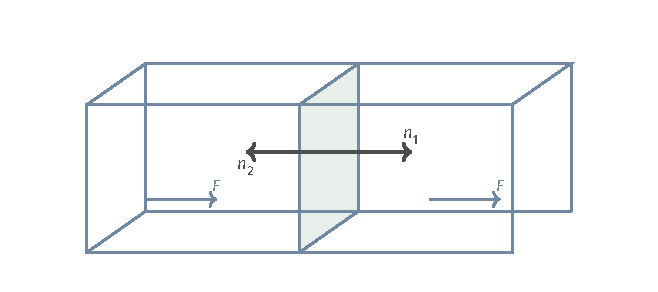
\includegraphics[width=112mm]{figures/00-shared/mathematical-preliminaries-upper/00-shared/tikz/chapter3-concept-processes/gauss-shared-face.pdf}
 \caption{两个相邻单位立方体共用绿色面，图用斜投影表示三维几何。取常场$F=(1,0,0)^\top$，共同面上两侧外法向为$n_1=(1,0,0)^\top$与$n_2=-n_1$，对应通量为$1,-1$，相加抵消。整体外向净通量也为零，与散度为零一致；一般区域的散度定理仍需要前述条件与证明。}
 \label{fig:analysis-process-gauss-shared-face}
\end{figure}

先用一个答案已知的计算核对散度定理。
\begin{example}[用散度定理核对球面面积]
设$B_R$是以原点为中心、半径$R>0$的球，边界球面取外法向。令$\bm F(\bm x)=\bm x/R$，它在整个$\mathbb R^3$上连续可微。
球面上$\bm n=\bm x/R=\bm F$，所以$\bm F^\top\bm n=1$，外向通量等于球面面积。
另一方面，$\operatorname{div}\bm F=3/R$，散度定理给出
\[
 \int_{\partial B_R}\bm F^\top\bm n\,\mathrm dS
 =\frac3R\operatorname{vol}(B_R)
 =\frac3R\cdot\frac{4\pi R^3}3=4\pi R^2.
\]
\end{example}
这里的球体积已在第~\ref{sec:classical-change-variables}节用球坐标算出；所得结果与第~\ref{sec:analysis-surface-integration}章直接参数化球面求得的面积一致。

定理要求$\bm F$在$\overline\Omega$的一个开邻域内连续可微。点源场在原点无定义，下面用它检查这一条件的作用。
\begin{example}[点源的通量]
\label{ex:analysis-point-source-flux}
在$\mathbb R^3\setminus\{\bm0\}$上取$\bm F(\bm x)=\bm x/\lVert\bm x\rVert_2^3$，记$r=\lVert\bm x\rVert_2$。由$\partial_jr=x_j/r$，
\[
 \begin{gathered}
\partial_j\Bigl(\frac{x_j}{r^3}\Bigr)=\frac1{r^3}-\frac{3x_j^2}{r^5}\\
\operatorname{div}\bm F=\frac3{r^3}-\frac{3r^2}{r^5}=0.
 \end{gathered}
\]
但在半径为$R$的球面上，外法向为$\bm x/R$，$\bm F^\top\bm n=1/R^2$，外向通量为$4\pi R^2/R^2=4\pi$。
这并不与散度定理矛盾：球体含有原点，而$\bm F$在原点无定义，定理的条件不满足。

对不含原点的球壳$R_1<r<R_2$，定理适用，左侧为零。外球面的外向通量为$4\pi$；内球面的外法向指向原点，通量为$-4\pi$；两者相加确为零。
\end{example}
所以以原点为中心的球面上的通量都是$4\pi$，与半径无关：场在原点以外处处无源，全部通量都来自原点处的点源。
静电学中，位于原点的点电荷$q$产生的电场是$\frac{q}{4\pi\varepsilon_0}\bm F$，其中$\varepsilon_0$为真空介电常数；它穿过以原点为中心的球面的通量为$q/\varepsilon_0$，这就是Gauss定律在点电荷上的形式。

\paragraph{散度是通量密度}

已证明的长方体情形，足以把散度一节的近似推导变成精确结论。
设$\bm F$在开集$U$上连续可微，$\bm a\in U$，$Q_h$是以$\bm a$为中心、边长为$h$的立方体；$h$足够小时$\overline{Q_h}\subseteq U$。由长方体上的Gauss公式，
\[
 \frac1{h^3}\int_{\partial Q_h}\bm F^\top\bm n\,\mathrm dS
 =\frac1{h^3}\int_{Q_h}\operatorname{div}\bm F\,\mathrm d\bm x.
\]
右侧是散度在$Q_h$上的平均值，它与$\operatorname{div}\bm F(\bm a)$的差不超过$\sup_{Q_h}|\operatorname{div}\bm F-\operatorname{div}\bm F(\bm a)|$。散度连续，所以$h\to0$时这个上界趋于零，平均值趋于$\operatorname{div}\bm F(\bm a)$。

这说明散度确实是“单位体积的净流出”的极限。把立方体换成以$\bm a$为中心的小球，用一般的Gauss公式可以得到同样的极限。小球的取法不依赖坐标轴，所以散度描述的是场本身的性质，不依赖坐标系的方向。

\subsection{Stokes公式与曲面的边界}

Gauss公式处理的是闭曲面围成的空间区域。另一类问题只给一张有边界的定向曲面，要比较曲面上的旋转累计与边界环流。这时使用旋度在曲面法向上的分量，不需要先把曲面补成闭曲面。

\subsubsection{Stokes公式}

在$z=0$平面上取向上法向时，旋度的法向分量$(\nabla\times\bm F)^\top\bm e_3$就是Green公式中的$Q_x-P_y$。

对空间中的弯曲曲面，可以把它切成许多很小的曲面片，每片近似是一小块平面。在法向为$\bm n$的小平面片上，边界环流约等于$(\nabla\times\bm F)^\top\bm n$乘面积。
各片采用相容定向时，相邻两片的公共边被沿相反方向走过，环流相消，只剩整张曲面的边界。
用桨轮的图像说：在曲面上各处放置转轴沿法向的小桨轮，它们感受到的旋转强度按面积累加，总和等于沿曲面边缘走一圈的环流。
Stokes公式把这一关系写成精确等式，同时要求法向与边界方向相容。
\begin{theorem}[Stokes定理]
\label{thm:multivariable-stokes}
设$S\subseteq\mathbb R^3$为紧致、可定向的分片$C^2$曲面，边界由有限条分段$C^1$简单闭曲线组成。
各光滑曲面片选取连续且片间定向相容的单位法向$\bm n$，边界采用其诱导方向。
若向量场$\bm F$在$S$的开邻域内连续可微，则\term{Stokes公式}（Stokes' theorem）给出
\begin{equation}
 \oint_{\partial S}\bm F^\top\,\mathrm d\bm r
 =\int_S(\nabla\times\bm F)^\top\bm n\,\mathrm dS.
 \label{eq:multivariable-stokes}
\end{equation}
\end{theorem}
这里的“可定向”要求各曲面片能相容地选择法向，使公共边上的诱导方向相反；有折角的接缝处不要求存在唯一法向。
两侧都为标量：左侧是原向量场的边界环流，右侧是其旋度穿过曲面的通量。

在一张参数曲面片上，可以把公式归结为参数平面上的Green公式。
设参数域$D$满足Green公式的区域条件，$\bm r(u,v)$在$D$的邻域内二阶连续可微、在内部正则且一一对应，并采用$\bm r_u\times\bm r_v$确定的定向。
还要求$\partial D$的正向经$\bm r$对应曲面片边界的诱导方向，从而可以把边界路径积分放到$\partial D$上计算。
这里的$u,v$是曲面的局部参数。记
\[
 \begin{aligned}
 A(u,v)&=\bm F(\bm r(u,v))^\top\bm r_u(u,v),\\
 B(u,v)&=\bm F(\bm r(u,v))^\top\bm r_v(u,v).
 \end{aligned}
\]

先处理左侧。若$(u(t),v(t))$沿$\partial D$行进，曲面边界上对应的点是$\bm r(u(t),v(t))$，由链式法则，其速度为$\bm r_uu'(t)+\bm r_vv'(t)$。
与$\bm F$取内积，得
\[
 \bm F^\top\mathrm d\bm r=A\,\mathrm du+B\,\mathrm dv,
\]
所以左侧等于参数平面上的路径积分
\[
 \oint_{\partial D}A\,\mathrm du+B\,\mathrm dv.
\]

再计算参数平面上Green公式右侧的被积函数$\partial_uB-\partial_vA$。记$\bm J_{\bm F}$为$\bm F$的Jacobian矩阵，其元素为$(\bm J_{\bm F})_{i,j}=\partial_jF_i$。由链式法则和乘积法则，
\[
 \begin{aligned}
 \partial_uB&=(\bm J_{\bm F}\bm r_u)^\top\bm r_v+\bm F^\top\bm r_{vu},\\
 \partial_vA&=(\bm J_{\bm F}\bm r_v)^\top\bm r_u+\bm F^\top\bm r_{uv},
 \end{aligned}
\]
其中$\bm J_{\bm F}$与$\bm F$在$\bm r(u,v)$处取值。$\bm r$二阶连续可微，混合偏导相等，$\bm r_{uv}=\bm r_{vu}$，所以两式相减时含二阶导数的项抵消。
剩下的两项可以改写为
\[
 \begin{aligned}
 (\bm J_{\bm F}\bm r_u)^\top\bm r_v&=\bm r_v^\top\bm J_{\bm F}\bm r_u,\\
 (\bm J_{\bm F}\bm r_v)^\top\bm r_u&=\bm r_v^\top\bm J_{\bm F}^\top\bm r_u,
 \end{aligned}
\]
于是
\[
 \partial_uB-\partial_vA=\bm r_v^\top(\bm J_{\bm F}-\bm J_{\bm F}^\top)\bm r_u.
\]

接下来把右端写成旋度。反对称矩阵$\bm W=\bm J_{\bm F}-\bm J_{\bm F}^\top$的元素为$\bm W_{i,j}=\partial_jF_i-\partial_iF_j$；逐个分量对照旋度的定义可以验证，对任意$\bm a\in\mathbb R^3$都有
\[
 \bm W\bm a=(\nabla\times\bm F)\times\bm a.
\]
再用混合积的轮换关系
\[
 \bm b^\top(\bm c\times\bm a)=\bm c^\top(\bm a\times\bm b)
\]
（两边都等于以$\bm a,\bm b,\bm c$为列的行列式），取$\bm a=\bm r_u$、$\bm b=\bm r_v$、$\bm c=\nabla\times\bm F$，得到
\[
 \partial_uB-\partial_vA
 =\bigl(\operatorname{curl}\bm F\bigr)(\bm r(u,v))^\top
   (\bm r_u\times\bm r_v).
\]
右端乘$\mathrm du\,\mathrm dv$，正是曲面通量积分（式~\eqref{eq:analysis-surface-flux}）中的被积项。

$A,B$由连续可微的$\bm F$与二阶连续可微的$\bm r$及其一阶导数复合、相乘而成，在$D$的邻域内连续可微，所以参数平面上的Green公式适用；它给出该曲面片上的Stokes公式。
对有限张相容定向的曲面片，公共边的路径积分相消，只剩整张曲面的边界。
一般分片曲面的完整论证还需核对曲面覆盖及接缝条件；以上推导只说明参数片上的机制，一般定理可参考向量微积分教材\scite{math-strang1991calculus}。

\paragraph{旋度分量是环流密度}

Stokes公式也给出旋度含义的精确形式。

设$\bm F$在$\bm a$附近连续可微，$\bm n$是单位向量，$D_\rho$是以$\bm a$为圆心、半径为$\rho$、垂直于$\bm n$并取法向$\bm n$的平面圆盘。由Stokes公式，
\[
 \frac1{\pi\rho^2}\oint_{\partial D_\rho}\bm F^\top\,\mathrm d\bm r
 =\frac1{\pi\rho^2}\int_{D_\rho}(\nabla\times\bm F)^\top\bm n\,\mathrm dS,
\]
右侧是$(\nabla\times\bm F)^\top\bm n$在圆盘上的平均值。旋度连续，所以$\rho\to0$时它趋于$(\nabla\times\bm F)(\bm a)^\top\bm n$。
因此，旋度沿$\bm n$的分量就是垂直于$\bm n$的微小圆周上的环流除以所围面积的极限。这正是桨轮图像所描述的量；圆盘的取法不依赖坐标轴，所以这一含义也不依赖坐标轴的选取。

\subsubsection{跨接曲面的选择}

Stokes公式的左侧只由有向边界和边界上的向量场决定。因此，若两张满足定理条件的定向曲面具有同一有向边界，
且$\bm F$在两张曲面附近都连续可微，则两张曲面上的旋度通量相等。
计算时可以选较简单的跨接曲面，但必须核对向量场定义域，不能让替换曲面穿过场的奇点。

这一结论也可以从Gauss公式得到印证。若$\bm F$二阶连续可微，前面已由混合偏导交换证明$\operatorname{div}(\operatorname{curl}\bm F)=0$。设两张跨接曲面恰好围成一个满足Gauss公式条件的区域，且$\bm F$在该区域闭包的开邻域内二阶连续可微。
区域的外法向在一张曲面上与所选法向相同，在另一张上相反；旋度场的散度为零，所以散度定理说明两张曲面上的旋度通量之差为零。

下面用同一个场在单位圆上比较两张跨接曲面。
\begin{example}[单位圆上的圆盘与半球面]
取$\bm F=(-y/2,x/2,0)^\top$，它在整个$\mathbb R^3$上连续可微，示例~\ref{ex:analysis-rigid-rotation-curl}已算出$\nabla\times\bm F=(0,0,1)^\top$。单位圆$\{x^2+y^2=1,\ z=0\}$采用从上方看逆时针的方向。

先取向上单位圆盘$S_1$。由示例~\ref{ex:analysis-hemisphere-induced-orientation}，它的诱导方向正是这一方向；旋度的法向分量为$1$，所以
\[
 \oint_{\partial S_1}\bm F^\top\,\mathrm d\bm r
 =\iint_{S_1}1\,\mathrm dS=\pi.
\]
直接计算左侧也得到同一结果：取$\gamma(t)=(\cos t,\sin t,0)^\top$，$0\leq t\leq2\pi$，则$\bm F(\gamma(t))^\top\gamma'(t)=\tfrac12(\sin^2t+\cos^2t)=\tfrac12$，积分为$\pi$。

再取外向上半单位球面$S_2$，同一例子说明它的诱导方向与$S_1$相同。
用第~\ref{sec:analysis-surface-integration}章的球面参数$(\varphi,\theta)$，$0\leq\varphi\leq\pi/2$，外法向为$\bm n=\bm x$，旋度的法向分量为$z=\cos\varphi$，面积元为$\sin\varphi\,\mathrm d\varphi\,\mathrm d\theta$，所以
\[
 \int_{S_2}(\nabla\times\bm F)^\top\bm n\,\mathrm dS
 =\int_0^{2\pi}\int_0^{\pi/2}\cos\varphi\sin\varphi\,\mathrm d\varphi\,\mathrm d\theta
 =2\pi\cdot\frac12=\pi,
\]
与圆盘上的结果相同。
\end{example}
若改用向下定向的圆盘，边界方向也必须反转，两个积分同时变号。


图~\ref{fig:analysis-process-stokes-spanning-surfaces}比较同一有向圆周的两张跨接曲面。替换曲面时，边界方向与场的定义域都要同时保留。
\begin{figure*}[!htbp]
 \centering
 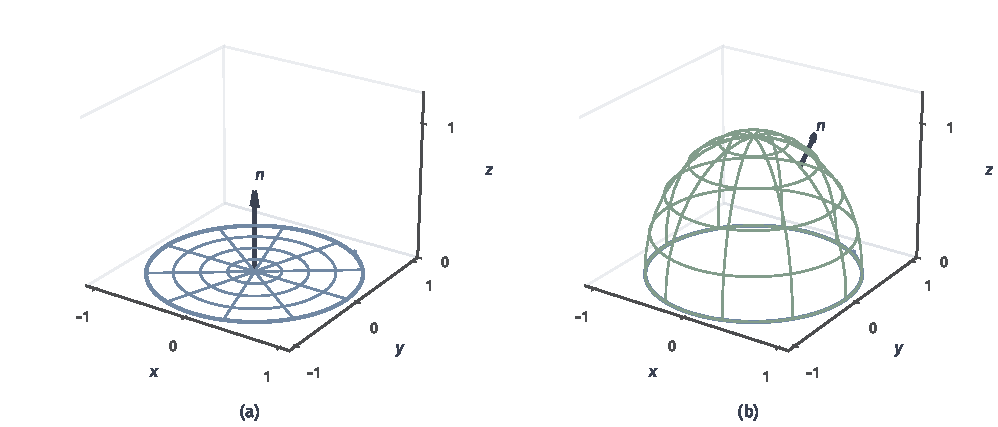
\includegraphics[width=169.0mm]{figures/00-shared/mathematical-preliminaries-upper/00-shared/matplotlib/chapter3-concept-processes/stokes-spanning-surfaces.pdf}
 \caption{(a) 向上单位圆盘；(b) 外向上半单位球面。蓝色边界均从上方看逆时针，黑箭头标记各自法向。对$F=(-y/2,x/2,0)^\top$，旋度恒为$(0,0,1)^\top$，两面上的旋度通量都为$\pi$。右面面积为$2\pi$而非$\pi$；相等的是法向分量的累计，不能把通量当成面积。}
 \label{fig:analysis-process-stokes-spanning-surfaces}
\end{figure*}

\subsection{分部积分与Green恒等式}

分部积分把导数从一个因子转移到另一个因子，同时留下边界上的贡献。Gauss公式给出它的多元形式。

设$\Omega$满足Gauss公式的区域条件，标量函数$u$与向量场$\bm F$在$\overline\Omega$的开邻域内都是$C^1$。逐坐标使用乘积法则，得到
\[
 \operatorname{div}(u\bm F)=\nabla u^\top\bm F+u\operatorname{div}\bm F.
\]
对两边积分，左侧用Gauss公式化为边界通量，再移项，得到
\[
 \int_\Omega u\operatorname{div}\bm F\,\mathrm dV
 =\int_{\partial\Omega}u\bm F^\top\bm n\,\mathrm dS
 -\int_\Omega\nabla u^\top\bm F\,\mathrm dV.
\]
若边界上$u=0$，或$\bm F$的法向分量为零，边界项消失；一般情况下必须保留它。

最常用的是$\bm F=\nabla v$的情形，它对应一元分部积分。设$u,w$在$[a,b]$上连续可微，一元分部积分
\[
 \int_a^bu\,w'\,\mathrm dx=[uw]_a^b-\int_a^bu'w\,\mathrm dx
\]
把一个因子的导数转给另一个因子，并留下端点项，可参考\BookChapterRef{chap:univariate-integration}{卷一“一元函数的积分”章}。

设$u$在$[a,b]$上连续可微、$v$二阶连续可微，取$w=v'$，得到
\[
 \int_a^bu\,v''\,\mathrm dx
 =u(b)v'(b)\cdot(+1)+u(a)v'(a)\cdot(-1)-\int_a^bu'v'\,\mathrm dx.
\]
这里把端点项$[uv']_a^b$拆开写：区间在右端点的外法向是$+1$，在左端点是$-1$。

推广到多元情形时，各项依次对应：$v''$换成$\Delta v$，$u'v'$换成梯度的内积$\nabla u^\top\nabla v$，两个端点换成边界曲面，“$v'$乘外法向$\pm1$”换成$v$沿外法向的方向导数$\nabla v^\top\bm n$。
\begin{theorem}[多元分部积分]
\label{thm:multivariable-integration-by-parts}
设$\Omega\subseteq\mathbb R^3$满足上述Gauss公式的区域条件。
若标量函数$u$在$\overline\Omega$的开邻域内连续可微，$v$在同一邻域内二阶连续可微，则
\begin{equation}
 \int_\Omega u\Delta v\,\mathrm d\bm x
 =\int_{\partial\Omega}u\nabla v^\top\bm n\,\mathrm dS
  -\int_\Omega\nabla u^\top\nabla v\,\mathrm d\bm x.
 \label{eq:multivariable-integration-by-parts}
\end{equation}
\end{theorem}
\begin{proof}
向量场$\bm F=u\nabla v$的第$j$个分量是$u\,\partial_jv$，它连续可微。由一元乘积法则，
$\partial_j(u\,\partial_jv)=\partial_ju\,\partial_jv+u\,\partial_j^2v$，对$j$求和得到
\[
 \operatorname{div}(u\nabla v)
 =\nabla u^\top\nabla v+u\Delta v.
\]
将它代入Gauss公式，再把$\nabla u^\top\nabla v$的区域积分移到等式另一侧，即得结论。
\end{proof}
对满足Green公式条件的平面区域，同样的证明改用平面通量公式（定理~\ref{thm:multivariable-planar-flux}）即可，边界上的面积元相应换成弧长元。
这一公式把$v$的二阶导数转为$u$与$v$的一阶导数，同时留下法向边界项；该项是否为零，要由具体的边界条件决定。

取$u=1$，公式化为
\[
 \int_\Omega\Delta v\,\mathrm d\bm x=\int_{\partial\Omega}\nabla v^\top\bm n\,\mathrm dS,
\]
也就是对梯度场$\nabla v$使用散度定理。下面在球上核对这一特例。
\begin{example}[球上平方范数的Laplace积分]
取以原点为中心、半径为$R$的球$B_R$和$v(\bm x)=\lVert\bm x\rVert_2^2$。
区域一侧，$\Delta v=6$是常数，所以
\[
 \int_{B_R}\Delta v\,\mathrm d\bm x=6\operatorname{vol}(B_R)=6\cdot\frac{4\pi R^3}3=8\pi R^3.
\]

边界一侧，球面上$\nabla v=2\bm x$，外法向为$\bm n=\bm x/R$，法向导数
\[
 \nabla v^\top\bm n=\frac{2\lVert\bm x\rVert_2^2}R=2R
\]
同样是常数，乘以球面面积得$2R\cdot4\pi R^2=8\pi R^3$。

两侧相等：$v$在球内各处的弯曲总量，等于它在球面上向外的增长率的累计。
\end{example}

边界项为零时，公式可以给出结构性的结论。下面用它说明Laplace方程的解由边界值唯一确定。
\begin{example}[Laplace方程的解由边界值决定]
设$\Omega$满足Gauss公式的区域条件，$w$在$\overline\Omega$的开邻域内二阶连续可微，在$\Omega$内$\Delta w=0$，在$\partial\Omega$上$w=0$。
在定理~\ref{thm:multivariable-integration-by-parts}中取$u=v=w$。左侧被积函数$w\Delta w$为零；边界项的被积函数含因子$w$，也为零。于是
\[
 \int_\Omega\lVert\nabla w\rVert_2^2\,\mathrm d\bm x=0.
\]
被积函数连续且非负；若它在某点为正，则在该点的一个邻域内为正，积分也为正。所以在开集$\Omega$上$\nabla w$恒为零。
$\Omega$是连通的开区域，所以$w$在$\Omega$上为常数；再由$w$在$\overline\Omega$上连续且在边界上为零，得$w\equiv0$。

现在设$v_1,v_2$都在$\overline\Omega$的开邻域内二阶连续可微，在$\Omega$内满足$\Delta v_1=\Delta v_2=0$，在$\partial\Omega$上取值相同。差$w=v_1-v_2$满足上面的全部条件，所以$v_1=v_2$。
\end{example}
按热传导的解释，稳定的温度分布由边界温度唯一决定。

若$u,v$都为$C^2$函数，交换分部积分公式中的$u,v$，再将两式相减，梯度内积项抵消，得到Green第二恒等式：
\begin{equation}
 \int_\Omega (u\Delta v-v\Delta u)\,\mathrm d\bm x
 =\int_{\partial\Omega}(u\nabla v-v\nabla u)^\top\bm n\,\mathrm dS.
 \label{eq:multivariable-green-second-identity}
\end{equation}
前面的分部积分公式也称Green第一恒等式。两式要求同样的区域条件和边界定向。第二式说明，在积分中把$\Delta$从$v$移到$u$上，差别只在边界项。

\paragraph{积分公式的比较}

本节各公式回答的都是同一类问题：导数在内部的积分与边界积分之间的关系。推导方式也相同：在小块上建立局部关系，再利用相容方向让内部边界相消。
它们的内部对象、边界对象和方向条件则各不相同。下表把一元基本定理与路径积分基本定理也列在一起，二者以区间或路径的两个端点为边界。
\begin{center}
\begin{tabular}{lll}
\toprule
公式 & 内部积分 & 边界积分\\
\midrule
一元基本定理 & 区间上的$f'$ & 端点值之差$f(b)-f(a)$\\
路径积分基本定理 & 路径上$\nabla\phi$的切向积分 & 端点值之差\\
Green环流形式 & 平面区域的$Q_x-P_y$ & 正向路径的切向积分\\
Gauss & 空间区域的散度 & 闭曲面的外向通量\\
Stokes & 定向曲面的旋度通量 & 诱导方向的路径环流\\
\bottomrule
\end{tabular}
\end{center}
对向上定向的平面曲面，Stokes公式还原为Green公式的环流形式；Green公式的通量形式则是二维的散度公式。
普通标量函数的区域积分不自动具有边界表达：要使用这些公式，须先找到满足条件的向量场，使其散度或旋度的相应分量等于被积函数。示例~\ref{ex:analysis-green-area-formula}的面积公式就是先选出满足$Q_x-P_y\equiv1$的场。

Stokes公式还解释了第~\ref{sec:multivariable-potential-path-independence}节中势函数的存在为何与定义域有关。设$\bm F$在开集$U\subseteq\mathbb R^3$上连续可微且$\nabla\times\bm F=\bm0$。若一条闭路径是$U$内某张满足定理条件的定向曲面的有向边界，则该闭路径上的环流等于旋度的通量，也就是零。
在星形域中，闭路径上各点与中心点之间的线段扫出一张锥面，它整个落在定义域内，不会碰到场的奇点；这与那里在星形域上构造势函数的结论一致。
穿孔平面上绕原点的单位圆则不同：在平面内，以它为边界的区域只能是单位圆盘，必然包含原点，而场在原点无定义；所以局部条件$Q_x-P_y=0$并不排除$2\pi$的环流（示例~\ref{ex:analysis-annulus-vortex-green}）。

使用这些公式时，要逐项核对连续可微性、分片规则的边界与定向。尤其要核对向量场是否在整个积分对象附近都有定义：穿孔平面上的涡旋场在原点无定义，不能把包含原点的圆盘直接代入Green公式；点源场也不能直接用于包含原点的球体（示例~\ref{ex:analysis-point-source-flux}）。

区域积分中可以忽略的边界，在边界积分中正是累计的对象。所以必须知道场在边界上的实际取值，并检查它能否连续可微地延拓，不能只凭区域内部的积分值推断边界积分。
若要降低导数或边界的规则性，还须另行建立弱导数、边界迹及相应的积分公式，不能沿用这里的公式而省去条件。

\FloatBarrier

\FloatBarrier
\section{本章小结}
\label{sec:integral-theorems-summary}

散度与旋度是边界累计的局部密度。连续可微向量场的散度$\sum_j\partial_jF_j$等于收缩立方体或小球上单位体积的外向净通量，也是Jacobian的迹；正值表示源，负值表示汇，散度为零只表示流入与流出平衡，不表示场为零。

三维场的旋度沿单位向量$\bm n$的分量，等于垂直于$\bm n$的微小圆周上逆时针环流除以面积的极限；平面场对应的标量是$Q_x-P_y$。

旋度与流线是否弯曲是两回事：剪切流的流线是直线而旋度不为零，涡旋场在原点以外流线弯曲而旋度为零。

Laplace算子$\Delta v=\operatorname{div}\nabla v$是Hessian的迹，度量一点的值与周围平均值之差；$C^2$时$\operatorname{curl}\nabla v=\bm0$与$\operatorname{div}\operatorname{curl}\bm F=0$来自混合偏导数的交换。

三个积分公式都由同一机制得到：在小块上建立局部关系，相容方向使内部公共边界的贡献相消。Green公式把平面区域上$Q_x-P_y$的积分化为正向边界上的环流，它的通量形式把散度的积分化为外向通量；正向边界要求区域总在行进方向的左侧，孔洞边界因而是顺时针。

Gauss公式把空间区域上散度的积分化为闭曲面上的外向通量。Stokes公式把定向曲面上旋度的通量化为诱导方向下的边界环流，平面情形还原为Green公式；具有同一有向边界的两张曲面给出相同的旋度通量，前提是场在两张曲面附近都连续可微。

区分闭曲面与有边界曲面：前者配外向通量和散度，后者配边界环流和旋度。由乘积法则与Gauss公式得到多元分部积分$\int_\Omega u\Delta v=\int_{\partial\Omega}u\nabla v^\top\bm n-\int_\Omega\nabla u^\top\nabla v$，交换$u,v$相减得到Green第二恒等式。边界项是否消失取决于边界条件：边界值为零时它消失，并由此推出Laplace方程的解由边界值唯一确定。

使用这些公式时要逐项检查：场在整个积分对象的闭包附近连续可微，边界分片规则，法向与边界方向相容。穿孔平面上的涡旋场与原点处的点源场说明，局部的零旋度或零散度不能越过场的奇点推出零环流或零通量。放宽光滑性或边界规则性，需要另行建立弱导数与相应的积分公式。


